\documentclass[]{book}
\usepackage{lmodern}
\usepackage{amssymb,amsmath}
\usepackage{ifxetex,ifluatex}
\usepackage{fixltx2e} % provides \textsubscript
\ifnum 0\ifxetex 1\fi\ifluatex 1\fi=0 % if pdftex
  \usepackage[T1]{fontenc}
  \usepackage[utf8]{inputenc}
\else % if luatex or xelatex
  \ifxetex
    \usepackage{mathspec}
  \else
    \usepackage{fontspec}
  \fi
  \defaultfontfeatures{Ligatures=TeX,Scale=MatchLowercase}
\fi
% use upquote if available, for straight quotes in verbatim environments
\IfFileExists{upquote.sty}{\usepackage{upquote}}{}
% use microtype if available
\IfFileExists{microtype.sty}{%
\usepackage{microtype}
\UseMicrotypeSet[protrusion]{basicmath} % disable protrusion for tt fonts
}{}
\usepackage[margin=1in]{geometry}
\usepackage{hyperref}
\hypersetup{unicode=true,
            pdftitle={Ecological Momentary Assessment in Mental Health Research},
            pdfauthor={Jeroen Ruwaard; Lisa Kooistra; Melissa Thong},
            pdfborder={0 0 0},
            breaklinks=true}
\urlstyle{same}  % don't use monospace font for urls
\usepackage{natbib}
\bibliographystyle{apa}
\usepackage{color}
\usepackage{fancyvrb}
\newcommand{\VerbBar}{|}
\newcommand{\VERB}{\Verb[commandchars=\\\{\}]}
\DefineVerbatimEnvironment{Highlighting}{Verbatim}{commandchars=\\\{\}}
% Add ',fontsize=\small' for more characters per line
\usepackage{framed}
\definecolor{shadecolor}{RGB}{248,248,248}
\newenvironment{Shaded}{\begin{snugshade}}{\end{snugshade}}
\newcommand{\KeywordTok}[1]{\textcolor[rgb]{0.13,0.29,0.53}{\textbf{#1}}}
\newcommand{\DataTypeTok}[1]{\textcolor[rgb]{0.13,0.29,0.53}{#1}}
\newcommand{\DecValTok}[1]{\textcolor[rgb]{0.00,0.00,0.81}{#1}}
\newcommand{\BaseNTok}[1]{\textcolor[rgb]{0.00,0.00,0.81}{#1}}
\newcommand{\FloatTok}[1]{\textcolor[rgb]{0.00,0.00,0.81}{#1}}
\newcommand{\ConstantTok}[1]{\textcolor[rgb]{0.00,0.00,0.00}{#1}}
\newcommand{\CharTok}[1]{\textcolor[rgb]{0.31,0.60,0.02}{#1}}
\newcommand{\SpecialCharTok}[1]{\textcolor[rgb]{0.00,0.00,0.00}{#1}}
\newcommand{\StringTok}[1]{\textcolor[rgb]{0.31,0.60,0.02}{#1}}
\newcommand{\VerbatimStringTok}[1]{\textcolor[rgb]{0.31,0.60,0.02}{#1}}
\newcommand{\SpecialStringTok}[1]{\textcolor[rgb]{0.31,0.60,0.02}{#1}}
\newcommand{\ImportTok}[1]{#1}
\newcommand{\CommentTok}[1]{\textcolor[rgb]{0.56,0.35,0.01}{\textit{#1}}}
\newcommand{\DocumentationTok}[1]{\textcolor[rgb]{0.56,0.35,0.01}{\textbf{\textit{#1}}}}
\newcommand{\AnnotationTok}[1]{\textcolor[rgb]{0.56,0.35,0.01}{\textbf{\textit{#1}}}}
\newcommand{\CommentVarTok}[1]{\textcolor[rgb]{0.56,0.35,0.01}{\textbf{\textit{#1}}}}
\newcommand{\OtherTok}[1]{\textcolor[rgb]{0.56,0.35,0.01}{#1}}
\newcommand{\FunctionTok}[1]{\textcolor[rgb]{0.00,0.00,0.00}{#1}}
\newcommand{\VariableTok}[1]{\textcolor[rgb]{0.00,0.00,0.00}{#1}}
\newcommand{\ControlFlowTok}[1]{\textcolor[rgb]{0.13,0.29,0.53}{\textbf{#1}}}
\newcommand{\OperatorTok}[1]{\textcolor[rgb]{0.81,0.36,0.00}{\textbf{#1}}}
\newcommand{\BuiltInTok}[1]{#1}
\newcommand{\ExtensionTok}[1]{#1}
\newcommand{\PreprocessorTok}[1]{\textcolor[rgb]{0.56,0.35,0.01}{\textit{#1}}}
\newcommand{\AttributeTok}[1]{\textcolor[rgb]{0.77,0.63,0.00}{#1}}
\newcommand{\RegionMarkerTok}[1]{#1}
\newcommand{\InformationTok}[1]{\textcolor[rgb]{0.56,0.35,0.01}{\textbf{\textit{#1}}}}
\newcommand{\WarningTok}[1]{\textcolor[rgb]{0.56,0.35,0.01}{\textbf{\textit{#1}}}}
\newcommand{\AlertTok}[1]{\textcolor[rgb]{0.94,0.16,0.16}{#1}}
\newcommand{\ErrorTok}[1]{\textcolor[rgb]{0.64,0.00,0.00}{\textbf{#1}}}
\newcommand{\NormalTok}[1]{#1}
\usepackage{longtable,booktabs}
\usepackage{graphicx,grffile}
\makeatletter
\def\maxwidth{\ifdim\Gin@nat@width>\linewidth\linewidth\else\Gin@nat@width\fi}
\def\maxheight{\ifdim\Gin@nat@height>\textheight\textheight\else\Gin@nat@height\fi}
\makeatother
% Scale images if necessary, so that they will not overflow the page
% margins by default, and it is still possible to overwrite the defaults
% using explicit options in \includegraphics[width, height, ...]{}
\setkeys{Gin}{width=\maxwidth,height=\maxheight,keepaspectratio}
\IfFileExists{parskip.sty}{%
\usepackage{parskip}
}{% else
\setlength{\parindent}{0pt}
\setlength{\parskip}{6pt plus 2pt minus 1pt}
}
\setlength{\emergencystretch}{3em}  % prevent overfull lines
\providecommand{\tightlist}{%
  \setlength{\itemsep}{0pt}\setlength{\parskip}{0pt}}
\setcounter{secnumdepth}{5}
% Redefines (sub)paragraphs to behave more like sections
\ifx\paragraph\undefined\else
\let\oldparagraph\paragraph
\renewcommand{\paragraph}[1]{\oldparagraph{#1}\mbox{}}
\fi
\ifx\subparagraph\undefined\else
\let\oldsubparagraph\subparagraph
\renewcommand{\subparagraph}[1]{\oldsubparagraph{#1}\mbox{}}
\fi

%%% Use protect on footnotes to avoid problems with footnotes in titles
\let\rmarkdownfootnote\footnote%
\def\footnote{\protect\rmarkdownfootnote}

%%% Change title format to be more compact
\usepackage{titling}

% Create subtitle command for use in maketitle
\newcommand{\subtitle}[1]{
  \posttitle{
    \begin{center}\large#1\end{center}
    }
}

\setlength{\droptitle}{-2em}

  \title{Ecological Momentary Assessment in Mental Health Research}
    \pretitle{\vspace{\droptitle}\centering\huge}
  \posttitle{\par}
  \subtitle{A Practical Introduction, with Examples in R (1st edition)}
  \author{Jeroen Ruwaard \\ Lisa Kooistra \\ Melissa Thong}
    \preauthor{\centering\large\emph}
  \postauthor{\par}
      \predate{\centering\large\emph}
  \postdate{\par}
    \date{2018-11-18}

% disable maketile temporarily (to get the cover before title - see frontpage.tex)
\let\oldmaketitle\maketitle
\AtBeginDocument{\let\maketitle\relax}

\usepackage{pdfpages}
\usepackage{booktabs}
\usepackage{makeidx}

\usepackage{float}
\floatplacement{figure}{H}
\makeindex
\usepackage[nottoc]{tocbibind}

\frontmatter

\begin{document}
\maketitle

\thispagestyle{empty}

\includepdf[fitpaper=false, pages=-]{images/cover/smallcover.jpg}

% restore maketile (disabled in preamble.tex to get the cover before
% title)
\let\maketitle\oldmaketitle
\maketitle

{
\setcounter{tocdepth}{1}
\tableofcontents
}
\chapter*{Preface}\label{preface}
\addcontentsline{toc}{chapter}{Preface}

Given known limitations of retrospective self-report questionnaires,
such as recall bias and poor generalizability of assessment results to
real-life situations, mental health researchers increasingly adopt
alternative assessment methods. One of the promising alternatives is
Ecological Momentary Assessment (EMA), in which emotions and behaviors
are repeatedly sampled in everyday life, through wearable electronic
devices.

Repeated measurement can reveal important characteristics of the
dynamics of phenomena, as illustrated by the cover of this book. With
EMA, we can tap into mental health processes that were, up to very
recently, unavailable to scientific research.

Conducting an EMA study, however, can be challenging. Researchers face a
dazzling array of options related to the electronic wearables, outcomes
selection, study design considerations, ethical and regulatory
constraints, data management, statistical analysis, and study reporting.
Although standards are emerging, clear guidelines for EMA research do
not - at present - exist. EMA studies have unique characteristics that
require specialist research skills, related to study design and
statistical analysis. This manual was written to fill this gap.

The manual provides a practical introduction to EMA-research. It was
written to aid beginning researchers of the Amsterdam School of Public
Health (APH), who are looking for practical advice in conducting EMA
studies. The manual provides an overview of EMA instruments, outcomes,
methods and analytic techniques, guidelines for EMA-studies, and a
catalogue of EMA research in the APH consortium.

This manual is available online at
\url{https://jruwaard.github.io/aph_ema_handbook/}. Sources are
available at \url{https://github.com/jruwaard/aph_ema_handbook}. Please
post your comments and suggestions there, or via e-mail, through
\href{mailto:aph.ema@ggzingeest.nl}{\nolinkurl{aph.ema@ggzingeest.nl}}.

This manual will be continuously updated. In citations, please include
explicit build dates, as in:

Ruwaard, J., Kooistra, L. and Thong, M. (2018). \emph{Ecological
Momentary Assessment in Mental Health Research: A Practical
Introduction, with Examples in R (1st edition - build 2018-11-18)}.
Amsterdam: APH Mental Health.

\mainmatter

\part{Introduction}\label{part-introduction}

\chapter{Introducing EMA}\label{introduction}

\section{What is EMA?}\label{what-is-ema}

\index{EMA} \index{EMA synonyms}
\index{EMA synonyms!Ambulatory Assessment}
\index{EMA synonyms!Experience Sampling}
\index{EMA synonyms!Ambulatory Self-reporting}
\index{EMA synonyms!Real-time Data Capturing}
\index{EMA synonyms!Continuous Unified Electronic Diary Method}
\index{EMA synonyms!Intensive-longitudinal Study Design}

Ecological Momentary Assessment (EMA) has many aliases. It is known as
`Experience Sampling' \citep{Larson1983}, `Ambulatory Assessment'
\citep{EbnerPriemer2009} or `Ambulatory Self-reporting'
\citep{Conner2012a}, `Real-time Data Capturing', the `Continuous Unified
Electronic Diary Method' \citep{EllisDavies2012}, and as the
`Intensive-longitudinal Study Design' \citep{Bolger2013}. The different
terms stress different aspects of EMA research. All, however, refer to
research methods that involve the \emph{repeated sampling of people's
current thoughts, emotions, behavior, physiological states, and context,
in their natural environment, typically (but not necessarily) via
electronic wearable devices} \citep{Shiffman2008}.

\subsection{Active versus Passive EMA}\label{active-versus-passive-ema}

\index{EMA!Passive EMA} \index{EMA!Observational EMA|see{Passive EMA}}
\index{EMA!Active EMA} \index{EMA!Self-report EMA|see{Active EMA}}

In EMA research, we distinguish two forms of data collection: 1) `Active
EMA', with which \emph{self-report} data are collected, and 2) `Passive
EMA', with which \emph{observational} data are collected. Active EMA
requires participants to consciously provide information, for example by
rating their current mood in response to a question that is prompted on
their smartphone (see Figure \ref{fig:activeema}). In passive EMA,
information is collected through wearables or log files without active
involvement of participants, for example on heart-rate, activity,
smartphone use or engagement on social media (see Figure
\ref{fig:passiveema}). Studies may combine active and passive EMA. A
study into sleep patterns, for example, may involve both a self-report
sleep diary and an accelerometer sensor \citep{Meijden2016}.

\begin{figure}

{\centering 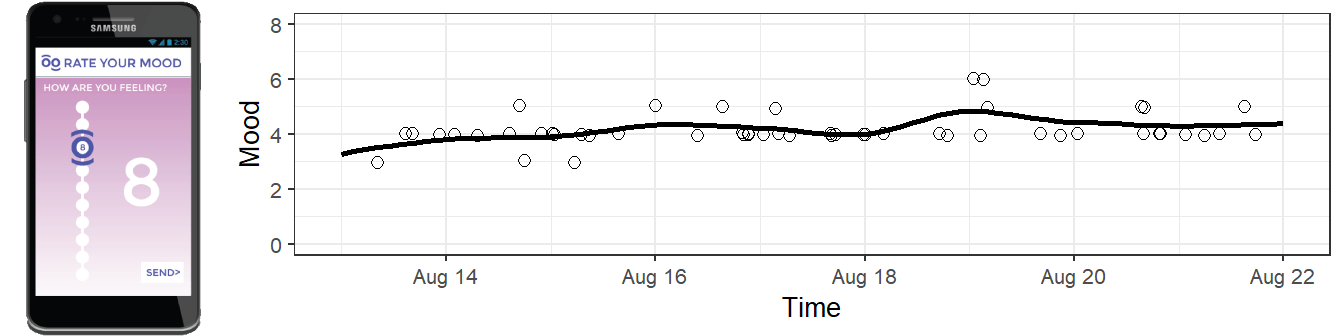
\includegraphics[width=0.95\linewidth]{EMA_files/figure-latex/activeema-1} 

}

\caption{Active EMA: data are collected by prompting questions to participants, for instance by using an EMA app such as Moodbuster. }\label{fig:activeema}
\end{figure}

\begin{figure}

{\centering 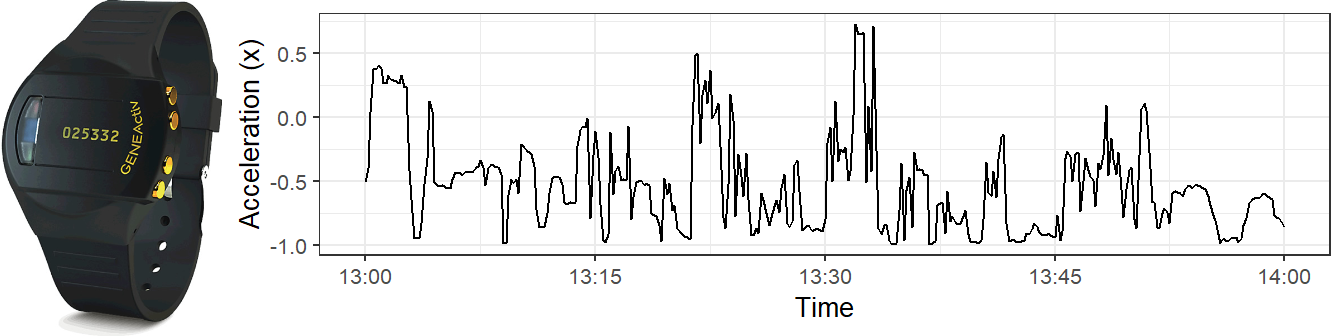
\includegraphics[width=1\linewidth]{EMA_files/figure-latex/passiveema-1} 

}

\caption{Passive EMA: data are collected automatically, for instance by a wearable device such as the GENEActiv accelerometer.}\label{fig:passiveema}
\end{figure}

\subsection{EMA Sampling}\label{ema-sampling}

\index{Sampling!Signal-contingent} \index{Sampling!Event-contingent}
\index{Sample plan|see{Sampling}}

EMA is further typified by the way in which data sampling is triggered.
EMA sampling may be triggered by a signal (signal-contingent sampling),
an event (event-contingent sampling), or a combination of both
\citep{Conner2012b}.

In \emph{signal-contingent sampling}, participants respond to questions
when they are prompted to do so by a signal (or `beeps', as these
signals are often called in the literature). In \emph{event-contingent
sampling}, study participants complete an assessment whenever a specific
event occurs, such as a panic attack or alcohol consumption.

Signal-contingent sampling can follow a fixed or a random scheme. In a
fixed scheme, participants are prompted at fixed time-points, for
example at 9:30, 12:30, and 16:30. In a random scheme, prompts are sent
at random time points, typically in pre-set intervals. For example,
participants could be prompted to complete two assessments per day, one
at a random time point between 10:00 and 14:00, and one at a random time
point between 14:00 and 16:00. Using pre-set intervals ensures that
participants do not receive several prompts within a limited time-frame
\citep{Piasecki2007}. In addition, it ensures that participants are not
bothered by prompts at inappropriate times (e.g., participants may not
appreciate prompts after 22:00 and before 7:30).

With `event-contingent sampling', the sample rate is determined by the
occurrence rate of the event. One way to implement this is to simply ask
study participants to complete a questionnaire whenever the event
occurs. When active EMA is combined with passive EMA, it may also be
possible to trigger event-based prompts automatically based on changes
in passive data, for example by triggering an EMA questionnaire
automatically whenever a significant change in activity level is
detected \citep{Smyth2003}.

\section{Why EMA?}\label{why-ema}

\subsection{To Minimize Recall Bias}\label{to-minimize-recall-bias}

\index{Recall bias}

In clinical research, self-report questionnaires are often used to
assess the presence and severity of symptoms in the recent past. While
useful, these retrospective self-reports are not without drawbacks,
since they tap into the memory of respondents, which can be distorted
\citep{Shiffman2008, Moore2016}. EMA circumvents this recall bias, by
asking participants to rate their \emph{current state}, rather than
asking them to reflect on past experiences.

\subsection{To Maximize Ecological
Validity}\label{to-maximize-ecological-validity}

\index{Ecological validity}

A key feature of EMA is the collection of data in real-world
environments, as participants go about their daily activities, as
opposed to data collection in controlled labs or research settings
\citep{Shiffman2008}. Thus, EMA data can be expected to result in
research findings that have better ecological validity and better
generalization to the subject's lived experience in real-world settings.
Practical applications derived from EMA data are therefore expected to
be more relevant to real-life situations.

\subsection{To Advance Ideographic
Research}\label{to-advance-ideographic-research}

\index{Nomothetic research} \index{Ideographic research}
\index{Intra-individual process|see{Ideographic research}}

In clinical research, a distinction is often made between
\emph{ideographic} and \emph{nomothetic} methods \citep{allport1937}.
Idiographic methods are those that ``aim to identify patterns of
behavior within the person across a population of experiences or
situations, and nomothetic methods{[}are{]} those that aim to identify
patterns of behavior across a population of individuals, rather than for
any given individual'' \citep{Conner2009}. The difference is important.
As is increasingly recognized, group-level findings do not necessarily
generalize to the individual members of the group, as shown by Figure
\ref{fig:idiographic} \citep{Hamaker2012}.

In contrast to more qualitative idiographic methods, such as interviews
and N = 1 case studies, EMA allows for the collection of large amounts
of quantitative data on the individual level. Thus, EMA offers a
quantitative method for idiographic research, measuring characteristics
of (unique) individuals across time and context \citep{Shiffman2008}.
This allows for a better understanding of the factors that account for
the variability within and between individuals.

\begin{figure}

{\centering 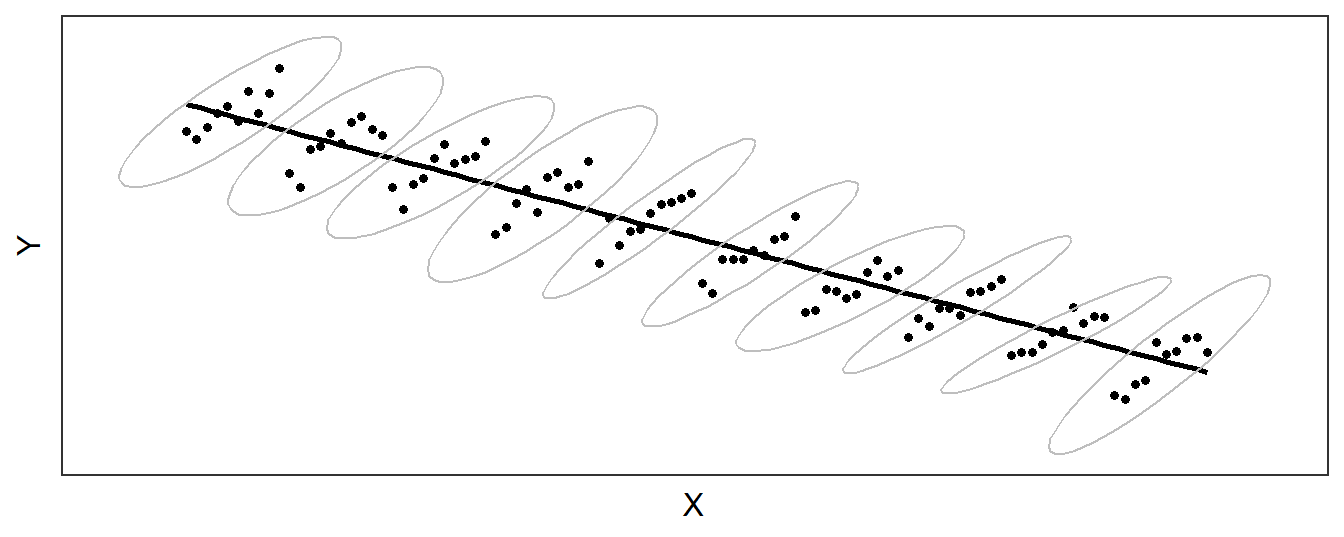
\includegraphics[width=1\linewidth]{EMA_files/figure-latex/idiographic-1} 

}

\caption{An illustration of how group-level and individual-level processes can differ dramatically: the relationship between x on y is negative in the group (as shown by the descending regression line), but positive for individuals (marked by ellipses).}\label{fig:idiographic}
\end{figure}

\subsection{To Understand the Dynamic Interplay between
Symptoms}\label{to-understand-the-dynamic-interplay-between-symptoms}

In the Network Theory of Psychopathology
\citep{Borsboom2013, Borsboom2017}, mental health disorders are
conceptualized as networks of psychopathology symptoms, in which
recurrent causal loops keep the network in a ``disorder'' state (e.g.,
sleeping problem -\textgreater{} fatigue -\textgreater{} rumination
-\textgreater{} sleeping problem). Network Theory encourages the
identification of patient-specific symptom networks, so that central
symptoms can be targeted with personalized interventions, to break the
self-sustaining loops. The identification of these networks requires
repeated assessments of symptoms in real life \citep[see,
e.g.,][]{Bringmann2015}, a task for which EMA is particularly well
suited.

\subsection{To Enable EMI}\label{to-enable-emi}

\index{Ecological Momentary Intervention}
\index{EMI|see{Ecological Momentary Intervention}}

EMA enables Ecological Momentary Interventions (EMI): interventions that
are provided to people during their everyday lives, in real time, and in
their natural settings \citep{heron2010}. If dynamic disease processes
can be adequately monitored in everyday-life through EMA, it should also
be possible to intervene when EMA data reflect clear changes in these
processes, in a way that is maximally effective given what is known
about the individual. A key term in the last sentence, however, is
``adequately''. We should be aware of the ``garbage-in/garbage-out''
principle. Before EMI's can be considered, the psychometric properties
of EMA measures should be demonstrated first.

\section{EMA Research Findings: A Birds-eye
View}\label{ema-research-findings-a-birds-eye-view}

The use of EMA in mental health research might seem novel but this
methodology has a long track record. Already in the 1980's, early
pioneers used electronic devices to elicit responses from study
participants to tap into (mental) health processes in everyday life
\citep[see, e.g.,][]{Csikszentmihalyi2014}. Recent years, however, have
witnessed a large increase in EMA research. Rapid technological
developments, a marked interest in the individual, and a wide
recognition of the need to study health-related processes in real-life
situations have all contributed to this.

EMA-based research in mental health has produced an impressive trove of
findings that have supported and, sometimes, challenged existing
theories on behavior. EMA data, whether collected as self-report or via
wearable device/sensor, have diagnostic, monitoring, management, or
intervention applications \citep{Patel2012, Aung2017, Evenson2015}. Its
feasibility for mental health research is evidenced by its use in
observational studies and randomized controlled trials on a wide range
of topics and populations. Below, we present a non-exhaustive summary of
systematic reviews and meta-analyses of EMA research.

\subsection{Active EMA}\label{active-ema}

\index{EMA!Active EMA}

Mood disorders have been well-studied using active EMA methods
\citep{Wenze2010}, with several reviews outlining recent findings in
depression \citep{Telford2012, Wichers2011, burton2013}, anxiety
disorders \citep{Walz2014}, and depression/bipolar disorder
\citep{AanhetRot2012}. The potential of EMA for use among young
populations showed promising results \citep{Dubad2018}. Innovations in
mobile devices have improved the feasibility and popularity of
ecological momentary interventions (EMIs) for anxiety and depression
\citep{schueller2017}. A systematic review and meta-analysis of EMIs
reported small to medium effects on mental health \citep{Versluis2016}.

EMA appears to be particularly well-suited to examine the role of
emotions in the development and maintenance of obesity and eating
disorders \citep{Engel2016}. Meta-analytic results suggest that negative
affect, rather than hunger, is associated with binge eating among
individuals with eating disorders \citep{Haedt2011, Haedt2012}. EMA
methods have also significantly contributed to the understanding of the
processes that drive substance use, cessation, and relapse, often in
contrast with theory-driven studies largely derived from global reports
collected through retrospective questionnaires
\citep{Shiffman2009, Swendsen2016}.

\subsection{Passive EMA}\label{passive-ema}

\index{EMA!Passive EMA}

Objective EMA data collected passively through bio-sensors, smart
devices, or context/environmental (e.g.~location) has been shown to be a
feasible and promising method for the longitudinal monitoring of
individuals with affective disorders \citep{Dogan2017, kirchner2016}.
The potential of passive sensing via smartphone for mental health
research are outlined in two reviews, encompassing the assessment of
health and well-being \citep{Cornet2017}, and the measuring,
understanding, and intervening in mental illness and maintaining mental
health \citep{Aung2017}. A systematic review and meta-analysis on
actigraphy reported diurnal variations in activity levels among
individuals with depression \citep{burton2013}. Compared with
traditional self-reports, passive sensing was reported to be less
intrusive and to result in more accurate data, while providing options
for continuous monitoring and feedback.

\subsection{Limitations}\label{limitations}

\index{Limitations}

While available reviews suggest that EMA is a feasible research method
that has the potential to make significant contributions to mental
health research, one significant drawback of EMA highlighted in several
reviews is the lack of high-quality studies. Other general limitations
considered include:

\begin{itemize}
\item
  Unclear generalizability of research findings due to selective samples
  \citep{burton2013}, and small sample sizes \citep{Dogan2017}
\item
  Unclear practice effects \citep{Telford2012}, and issues related to
  reactivity \citep{Shiffman2009}
\item
  Issues related to the feasibility and tolerability of prolonged and
  intense data periods of data collection \citep{Wichers2011}
\item
  Issues of privacy, ethics and informed consent \citep{Cornet2017}
\item
  Changing responsibilities of researchers and clinicians in EMA
  studies, e.g.~in suicide ideation research \citep{Wenze2010}
\item
  Unresolved methodological issues \citep{Dubad2018}
\end{itemize}

\index{EMA research!Anxiety disorders}
\index{EMA research!Eating disorders}
\index{EMA research!Mood disorders}
\index{EMA research!Substance-related disorders}
\index{EMA research!Mental health/ Well-being}

\begin{longtable}[]{@{}ll@{}}
\caption{\label{tab:emareviews} A selection of reviews of EMA studies
targeting various mental health conditions}\tabularnewline
\toprule
\begin{minipage}[b]{0.33\columnwidth}\raggedright\strut
\textbf{Topic} / \textbf{Author (Year)}\strut
\end{minipage} & \begin{minipage}[b]{0.61\columnwidth}\raggedright\strut
\textbf{Summary}\strut
\end{minipage}\tabularnewline
\midrule
\endfirsthead
\toprule
\begin{minipage}[b]{0.33\columnwidth}\raggedright\strut
\textbf{Topic} / \textbf{Author (Year)}\strut
\end{minipage} & \begin{minipage}[b]{0.61\columnwidth}\raggedright\strut
\textbf{Summary}\strut
\end{minipage}\tabularnewline
\midrule
\endhead
\begin{minipage}[t]{0.33\columnwidth}\raggedright\strut
\textbf{Anxiety disorders}\strut
\end{minipage} & \begin{minipage}[t]{0.61\columnwidth}\raggedright\strut
\strut
\end{minipage}\tabularnewline
\begin{minipage}[t]{0.33\columnwidth}\raggedright\strut
\citet{Walz2014}\strut
\end{minipage} & \begin{minipage}[t]{0.61\columnwidth}\raggedright\strut
Provides insights to the temporal variability of symptoms, and
associations between daily affect, behaviors, and situational cues.
Discusses the combination of EMA and ambulatory assessment of
physiological variables in treatment evaluations.\strut
\end{minipage}\tabularnewline
\begin{minipage}[t]{0.33\columnwidth}\raggedright\strut
\citet{schueller2017}\strut
\end{minipage} & \begin{minipage}[t]{0.61\columnwidth}\raggedright\strut
Provides an overview of the distinction of EMIs from other types of
treatment. Also discusses the considerations of conducting EMI research,
such as design, deployment, and evaluation.\strut
\end{minipage}\tabularnewline
\begin{minipage}[t]{0.33\columnwidth}\raggedright\strut
\textbf{Eating disorders}\strut
\end{minipage} & \begin{minipage}[t]{0.61\columnwidth}\raggedright\strut
\strut
\end{minipage}\tabularnewline
\begin{minipage}[t]{0.33\columnwidth}\raggedright\strut
\citet{Engel2016}\strut
\end{minipage} & \begin{minipage}[t]{0.61\columnwidth}\raggedright\strut
An overview of studies on eating disorders, obesity, and bariatric
surgery using EMA.\strut
\end{minipage}\tabularnewline
\begin{minipage}[t]{0.33\columnwidth}\raggedright\strut
\textbf{Mood disorders}\strut
\end{minipage} & \begin{minipage}[t]{0.61\columnwidth}\raggedright\strut
\strut
\end{minipage}\tabularnewline
\begin{minipage}[t]{0.33\columnwidth}\raggedright\strut
\citet{AanhetRot2012}\strut
\end{minipage} & \begin{minipage}[t]{0.61\columnwidth}\raggedright\strut
Provides an overview of EMA studies on correlates of mood, treatment
effects, residual symptoms of remitted patients, pediatric populations,
MDD/BD specificity, and links with neuroscience.\strut
\end{minipage}\tabularnewline
\begin{minipage}[t]{0.33\columnwidth}\raggedright\strut
\citet{Aung2017}\strut
\end{minipage} & \begin{minipage}[t]{0.61\columnwidth}\raggedright\strut
Provides a conceptual review of passive sensing techniques for
measuring, understanding, and treatment of mental illness.\strut
\end{minipage}\tabularnewline
\begin{minipage}[t]{0.33\columnwidth}\raggedright\strut
\citet{burton2013}\strut
\end{minipage} & \begin{minipage}[t]{0.61\columnwidth}\raggedright\strut
Focuses on diurnal variations in activity levels among depressed
individuals.\strut
\end{minipage}\tabularnewline
\begin{minipage}[t]{0.33\columnwidth}\raggedright\strut
\citet{Telford2012}\strut
\end{minipage} & \begin{minipage}[t]{0.61\columnwidth}\raggedright\strut
Identifies six themes of EMA research in MDD: methodology, positive and
negative affect, cortisol secretion, antidepressant treatment, work
performance, and genetic risk factors.\strut
\end{minipage}\tabularnewline
\begin{minipage}[t]{0.33\columnwidth}\raggedright\strut
\citet{Wenze2010}\strut
\end{minipage} & \begin{minipage}[t]{0.61\columnwidth}\raggedright\strut
Provides an overview of EMA in mood disorder research comprising
techniques used, types of population assessed, types of research
questions, and a discussion of the potential of EMA in treatment
settings.\strut
\end{minipage}\tabularnewline
\begin{minipage}[t]{0.33\columnwidth}\raggedright\strut
\citet{Wichers2011}\strut
\end{minipage} & \begin{minipage}[t]{0.61\columnwidth}\raggedright\strut
Provides an overview for the potential clinical application of EMA in
the diagnostic and treatment of MDD.\strut
\end{minipage}\tabularnewline
\begin{minipage}[t]{0.33\columnwidth}\raggedright\strut
\citet{Versluis2016}\strut
\end{minipage} & \begin{minipage}[t]{0.61\columnwidth}\raggedright\strut
Provides an overview of interventions (EMI) addressing anxiety,
depression, and perceived stress on positive psychological
outcomes.\strut
\end{minipage}\tabularnewline
\begin{minipage}[t]{0.33\columnwidth}\raggedright\strut
\citet{Dubad2018}\strut
\end{minipage} & \begin{minipage}[t]{0.61\columnwidth}\raggedright\strut
Provides an overview of the feasibility and clinical impact of
mood-monitoring applications targeting young populations (10-24 years
old).\strut
\end{minipage}\tabularnewline
\begin{minipage}[t]{0.33\columnwidth}\raggedright\strut
\textbf{Substance-related disorders}\strut
\end{minipage} & \begin{minipage}[t]{0.61\columnwidth}\raggedright\strut
\strut
\end{minipage}\tabularnewline
\begin{minipage}[t]{0.33\columnwidth}\raggedright\strut
\citet{Shiffman2009}\strut
\end{minipage} & \begin{minipage}[t]{0.61\columnwidth}\raggedright\strut
Review of processes that drive substance use, cessation, and relapse,
sometimes in contrast with theory-driven studies that are largely
derived from global reports collected through questionnaires.\strut
\end{minipage}\tabularnewline
\begin{minipage}[t]{0.33\columnwidth}\raggedright\strut
\citet{Swendsen2016}\strut
\end{minipage} & \begin{minipage}[t]{0.61\columnwidth}\raggedright\strut
Conceptual review of the use of mobile technologies for research on
addiction and its treatment.\strut
\end{minipage}\tabularnewline
\begin{minipage}[t]{0.33\columnwidth}\raggedright\strut
\textbf{Mental health/ Well-being}\strut
\end{minipage} & \begin{minipage}[t]{0.61\columnwidth}\raggedright\strut
\strut
\end{minipage}\tabularnewline
\begin{minipage}[t]{0.33\columnwidth}\raggedright\strut
\citet{Cornet2017}\strut
\end{minipage} & \begin{minipage}[t]{0.61\columnwidth}\raggedright\strut
Outlines the potential and challenges of passive sensing to detect
status change and behavior change following feedback on behavior.\strut
\end{minipage}\tabularnewline
\begin{minipage}[t]{0.33\columnwidth}\raggedright\strut
\citet{kirchner2016}\strut
\end{minipage} & \begin{minipage}[t]{0.61\columnwidth}\raggedright\strut
Provides an overview of `geographically explicit momentary assessment'
(GEMA) research to enrich EMA research in mental health and
well-being.\strut
\end{minipage}\tabularnewline
\begin{minipage}[t]{0.33\columnwidth}\raggedright\strut
\citet{Dogan2017}\strut
\end{minipage} & \begin{minipage}[t]{0.61\columnwidth}\raggedright\strut
Provides an overview of studies that combine subjective ratings with
objective EMA-data collected using smartphone-based systems.\strut
\end{minipage}\tabularnewline
\bottomrule
\end{longtable}

\section{What is in this Manual?}\label{what-is-in-this-manual}

This manual comprises six parts, in which various aspects of EMA
research are discussed.

\begin{itemize}
\item
  Chapter \ref{rstudio}, the second chapter of \textbf{Part I},
  introduces R, the statistical program that is an indispensable tool
  for the EMA researcher.
\item
  \textbf{Part II} focuses on EMA study design (Chapter \ref{methods}),
  and EMA data management (Chapter \ref{datamanagement}).
\item
  \textbf{Part III} details the momentary assessment of two specific
  outcomes: Mood (Chapter \ref{mood}) and Activity (Chapter
  \ref{activity}).
\item
  \textbf{Part IV} discusses EMA data analysis techniques: Feature
  Extraction (Chapter \ref{features}), and Mixed Modeling (Chapter
  \ref{lmm}).
\item
  In \textbf{part V}, the application of the preceding material is
  illustrated in a case study, in which EMA is used to detect early
  warnings signs of depression (Chapter \ref{csd}).
\item
  \textbf{Part VI} provides three catalogues of EMA resources. Chapter
  \ref{catalogue} lists EMA research groups within APH, chapter
  \ref{ema-instruments-catalogue} lists EMA instruments that were found
  to be in use among APH researchers, and Chapter \ref{rcat} summarizes
  useful R extensions (packages) for EMA data analysis.
\end{itemize}

\chapter{Introducing R \& RStudio}\label{rstudio}

\index{R and RStudio}

In this chapter, you will learn how to install and use two programs that
are indispensable for the management and analysis of EMA data: R and
RStudio.

\section{What are R and RStudio?}\label{what-are-r-and-rstudio}

R is a programming language and software environment for statistical
computing and data visualization. RStudio is a powerful user interface
to R. It has many useful features that greatly simplify R-work. We
strongly advise you to adopt the R/RStudio-combo.

\section{Why R?}\label{why-r}

\index{R and RStudio!Why R}

R, you may have been told, is for data scientists, methodologists, and
scientific programmers only. It has a steep learning curve. If you are
trained in SPSS, it will take time to become as productive in R as in
SPSS. Why then, should you invest in R?

\begin{itemize}
\item
  Unlike SPSS, R is free of charge. It does not eat up your budget. Why
  pay for something that you can get for free?
\item
  R is cutting-edge. Methodological innovations first appear in R.
  Network analyses, for example, can be run in R, but not (yet) in SPSS.
  For some analyses, you need this alternative.
\item
  Mastering R improves your connection to the statisticians in your
  team. They probably prefer R over SPSS. It is more efficient and less
  error-prone to all speak the same language.
\item
  R is great for data-management. Clinical research, and especially EMA
  research, requires hundreds of operations on multiple raw data files.
  R excels at that. SPSS, frankly, does not. If you care about
  reproducible research (which you should), R can be a great help in
  putting it into practice.
\item
  R can be used at different levels. If you want to be a basic user,
  that's fine. However, if you want to dive deeper, you will find that
  you can easily do so. You can study source code to understand a
  particular technique better. You can code new functions. R allows you
  to grow.
\item
  R's user base is expanding every year. Chances are high that R will be
  the standard in your next workplace. R will look great on your CV.
\end{itemize}

You don't have to be a programmer or methodologist to use R. Yes, it
takes time to unlock its full potential, but you should be able to run
basic analyses in it within a week. This chapter will get you started.

\section{Installing R \& RStudio}\label{installing-r-rstudio}

\index{R and RStudio!Installing}

Both R and RStudio are available, at no costs, for all major operating
systems.

\begin{itemize}
\item
  Download R from the Comprehensive R Archive Network (CRAN), at
  \url{https://cran.r-project.org/bin/}
\item
  Download RStudio from \url{http://rstudio.org}
\end{itemize}

Install R first, and RStudio second. If you install the programs in this
order, RStudio will automatically find R on your computer.

If you installed R or RStudio previously, please update. This manual
assumes you will be working with version 3.4.2 (or higher) of R, and
version 1.1.414 (or higher) of RStudio.

\section{Interacting with R through the RStudio
Console}\label{interacting-with-r-through-the-rstudio-console}

\index{R and RStudio!Console}

If you open RStudio, you will be presented with the interface shown in
Figure \ref{fig:r-interface}. RStudio's main window is divided in four
panes (sub-windows), which further contain several tabbed windows.

\begin{figure}

{\centering 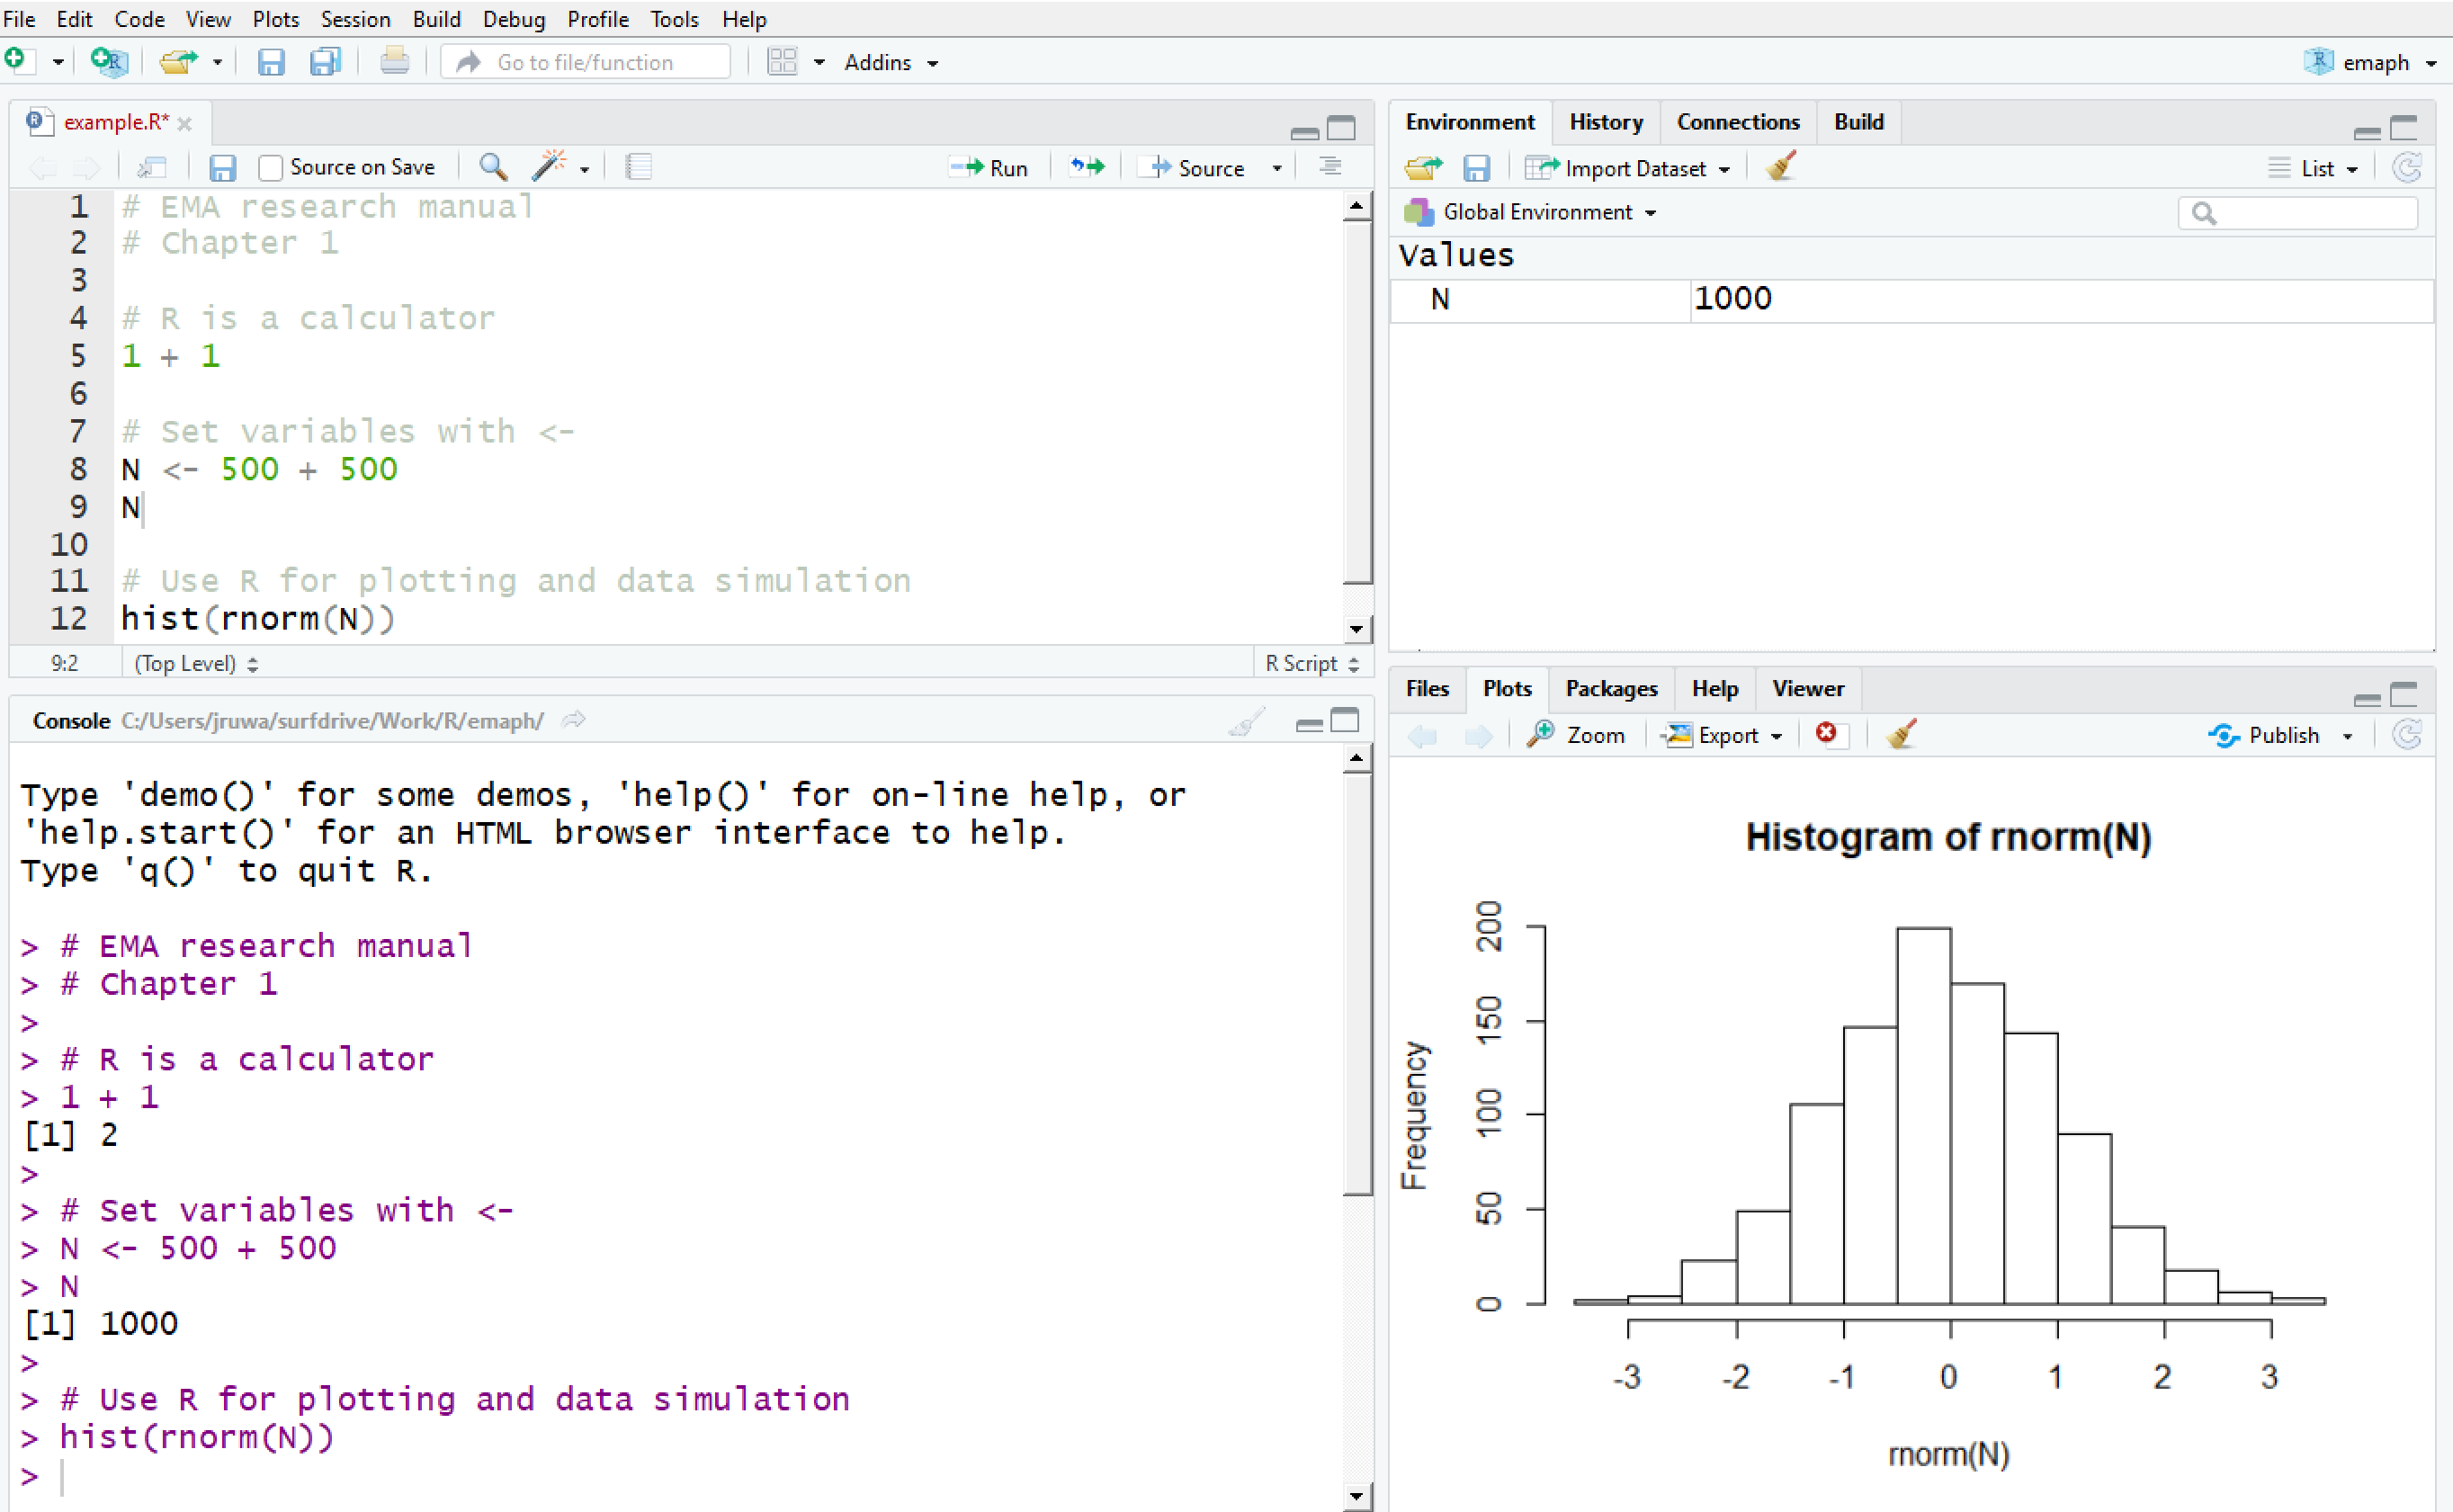
\includegraphics[width=0.98\linewidth]{images/R/rstudio} 

}

\caption{The RStudio Interface}\label{fig:r-interface}
\end{figure}

Commands are sent to R in the bottom-left pane, named ``Console''. To
test this, move your cursor to the bottom line, immediately after the
prompt sign (\texttt{\textgreater{}}). Next, type the statement below
(note that \texttt{\#} denotes a comment line; R ignores it, so there is
no immediate need to type that). To execute, press \texttt{Enter}.

R will execute the command and return the answer back to the console.

\begin{Shaded}
\begin{Highlighting}[]
\CommentTok{# R is a calculator.}
\DecValTok{1} \OperatorTok{+}\StringTok{ }\DecValTok{1}
\end{Highlighting}
\end{Shaded}

Results of calculations can be saved into variables, by making use of
the assignment operator (\texttt{\textless{}-}). If you type the name of
a variable, R returns its value.

\begin{Shaded}
\begin{Highlighting}[]
\CommentTok{# Use <- to declare and set a variable.}
\NormalTok{N <-}\StringTok{ }\DecValTok{50} \OperatorTok{+}\StringTok{ }\DecValTok{50}
\NormalTok{N}
\CommentTok{#> [1] 100}
\end{Highlighting}
\end{Shaded}

To understand why R is such a popular tool for statistical computing,
consider the following command, which, in one line, 1) uses the variable
N, just created, to 2) generate 100 random numbers from the normal
distribution, and 3) plot a histogram of these numbers.

\begin{Shaded}
\begin{Highlighting}[]
\CommentTok{# Plot the histogram of a sample from the normal distribution.}
\KeywordTok{hist}\NormalTok{(}\KeywordTok{rnorm}\NormalTok{(N))}
\end{Highlighting}
\end{Shaded}

The plot appears in the bottom-right pane, as in Figure
\ref{fig:r-interface}.

\section{Writing R-scripts}\label{writing-r-scripts}

\index{R and RStudio!Scripts}

Working in the console is a great way to interactively explore R and
data, but what if you want to save a particularly useful chain of
statements? For this, you can use a script file.

To create a script file, use the RStudio menu:
\texttt{File\ \textgreater{}\ New\ File\ \textgreater{}\ R\ Script}.
This will open a new tab in the top-left pane of RStudio, where you can
edit the script.

\begin{itemize}
\item
  In the script window, type all statements that you have been entering
  in the console in the previous section.
\item
  Next, select all lines in the script.
\item
  Press \texttt{Ctrl+Enter} to run the script.
\end{itemize}

All commands in the script are executed. The commands are echoed in the
console pane, and results are shown immediately, as was the case before,
when you typed the commands in the console yourself.

Scripts can also be run line by line. Move the cursor to the line you
want to run, and press \texttt{Ctrl+Enter}. The line is copied to the
console and executed, and the cursor in the script will move to the next
line, allowing you to walk through the script, step by step.

\section{Importing Your Data}\label{importing-your-data}

\index{R and RStudio!Data import}

Something that confuses new RStudio users, who are more familiar with
SPSS, is that it is not obvious how to import data into RStudio. In
SPSS, the data are in plain sight. In R, you first have to import the
data.

\subsection{Using RStudio Menus to Import
Data}\label{using-rstudio-menus-to-import-data}

One way to load data into R is to use RStudio's data import wizard.
Follow the steps below to see how this works with data stored in a
comma-separated-values (csv) format, a common data format to which many
programs, including SPSS and Excel, can export data to.

\begin{itemize}
\item
  Download the example csv data file at
  \url{https://tinyurl.com/yczmjdat} (or create a csv-version of one of
  your own data files).
\item
  In RStudio's menu, choose
  \texttt{File\ \textgreater{}\ Import\ Dataset\ \textgreater{}\ From\ Text\ (base)}.
\item
  In the window that appears, click on \texttt{Browse} to locate the
  csv- file on your computer, and click \texttt{Import} in the next
  window (see Figure \ref{fig:r-import}).
\end{itemize}

RStudio shows the data, in tabular view, in the top-left window, ready
for analysis. You will also find a new entry in the
\texttt{Environment}-tab in the top-right pane. When you click the small
arrow, at the left of the name, you will see a brief summary of the
contents of the data.

\begin{figure}

{\centering 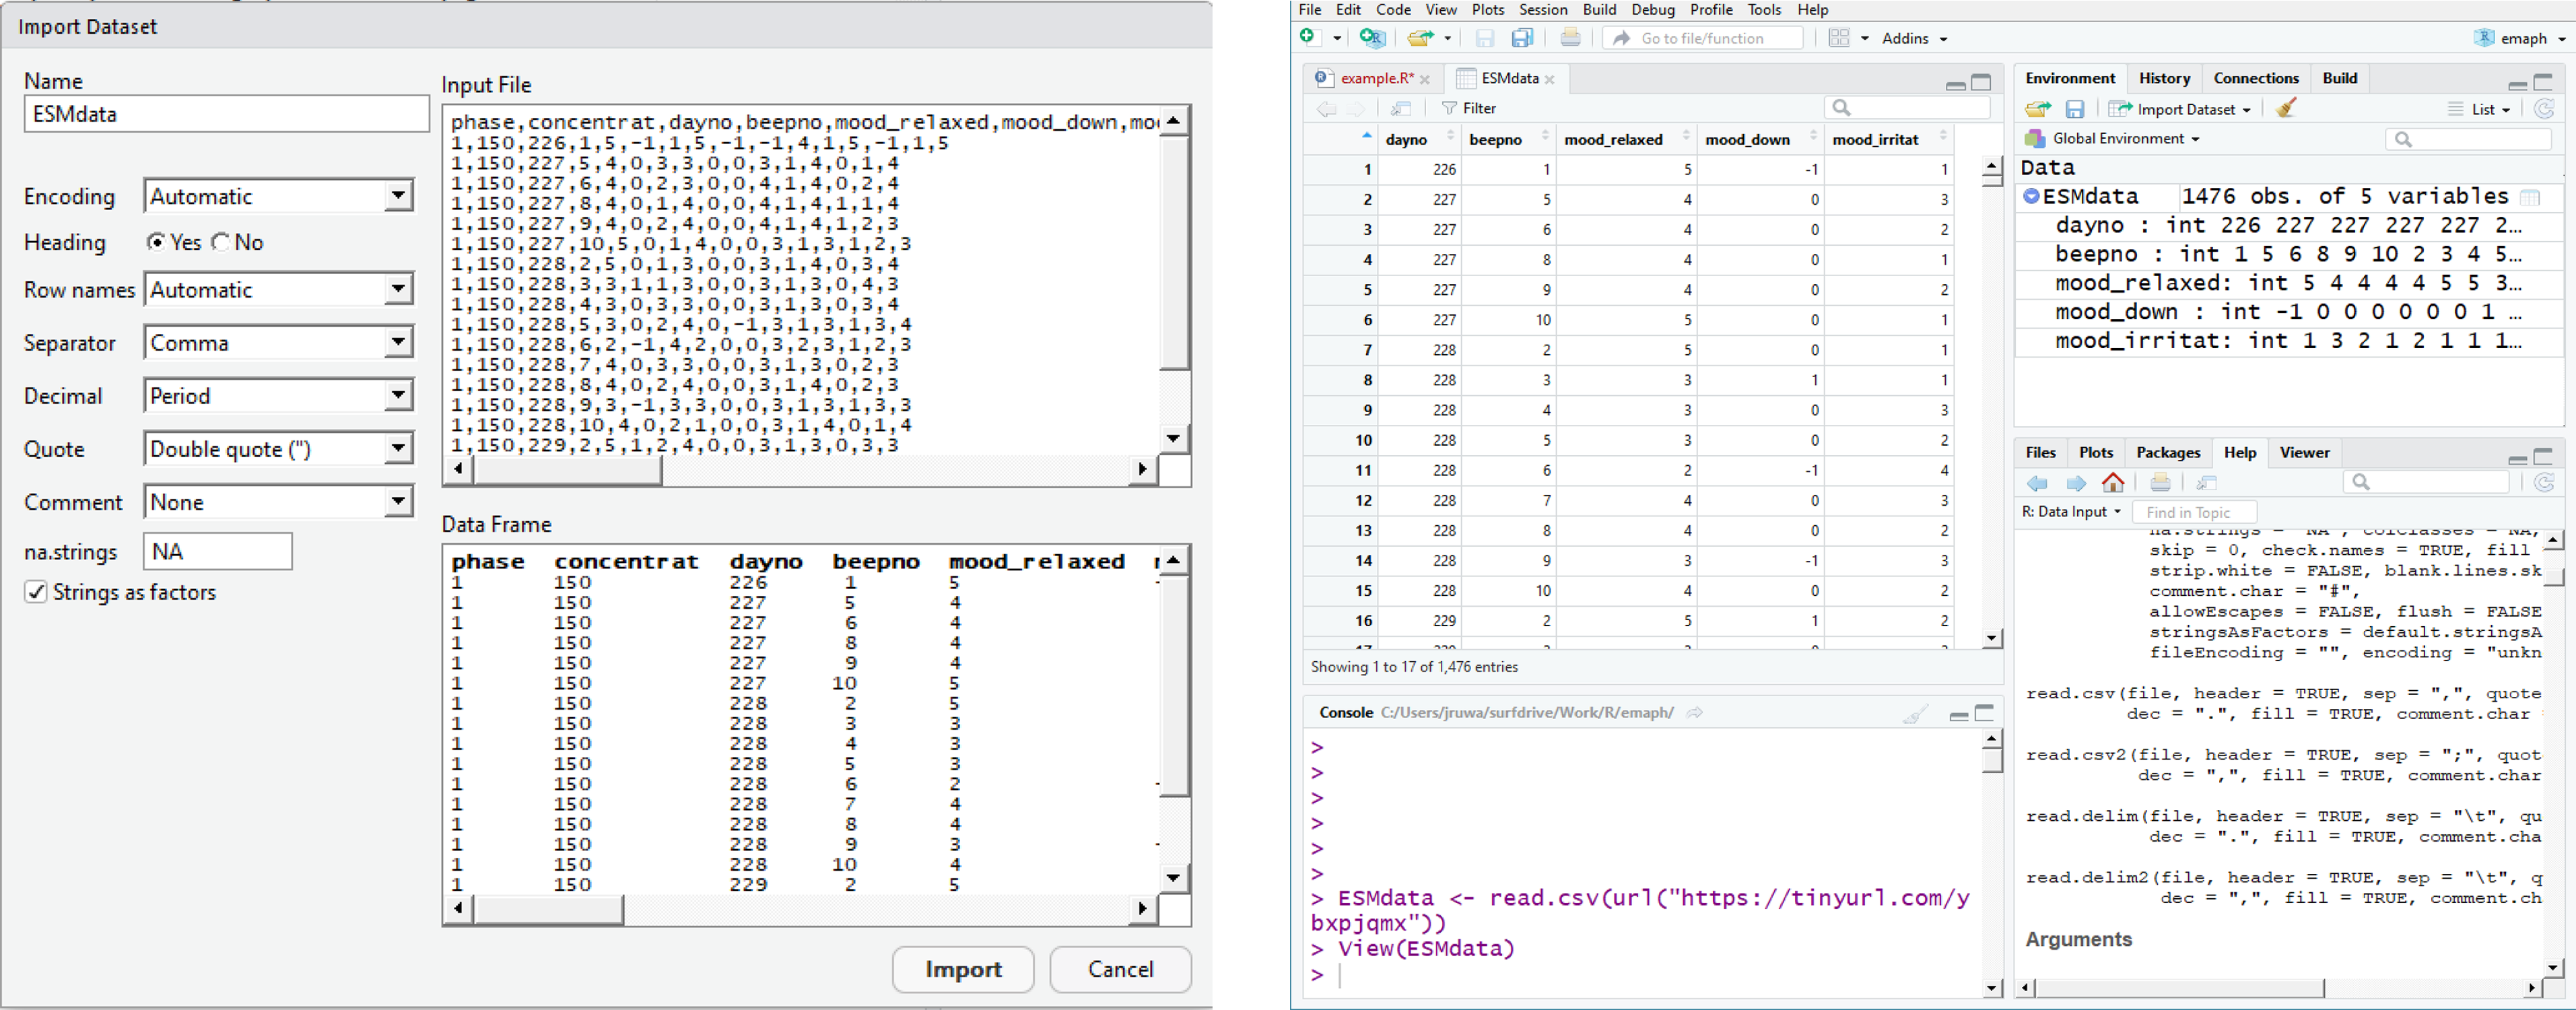
\includegraphics[width=0.98\linewidth]{images/R/csv_import} 

}

\caption{RStudio's CSV import wizard.}\label{fig:r-import}
\end{figure}

\subsection{Using Functions to Import
Data}\label{using-functions-to-import-data}

While RStudio's Data import wizard is useful, you will probably use it
less over time. Most likely, you will convert to using the more
efficient R commands to import data. For example, it takes only a single
line to download and import the example data.

\begin{Shaded}
\begin{Highlighting}[]
\CommentTok{# Import csv-data, from the internet.}
\NormalTok{ESMdata <-}\StringTok{ }\KeywordTok{read.csv}\NormalTok{(}\KeywordTok{url}\NormalTok{(}\StringTok{"https://tinyurl.com/yczmjdat"}\NormalTok{), }\DataTypeTok{row.names =} \OtherTok{NULL}\NormalTok{)}
\end{Highlighting}
\end{Shaded}

\subsection{Accessing your Data}\label{accessing-your-data}

\index{R and RStudio!Data access}

Since the data is now in the environment (under the name
\texttt{ESMdata}), you can use it in other R commands. For example, to
produce a more detailed summary of the first four columns of
\texttt{ESMdata}, you type:

\begin{Shaded}
\begin{Highlighting}[]
\CommentTok{# Summarize data.}
\KeywordTok{summary}\NormalTok{(ESMdata)}
\NormalTok{     dayno           beepno       mood_relaxed     mood_down      }
\NormalTok{ Min.   }\OperatorTok{:}\StringTok{  }\FloatTok{1.0}\NormalTok{   Min.   }\OperatorTok{:}\StringTok{ }\FloatTok{1.00}\NormalTok{   Min.   }\OperatorTok{:}\FloatTok{1.000}\NormalTok{   Min.   }\OperatorTok{:-}\FloatTok{3.0000}  
\NormalTok{ 1st Qu.}\OperatorTok{:}\StringTok{ }\FloatTok{61.0}\NormalTok{   1st Qu.}\OperatorTok{:}\StringTok{ }\FloatTok{3.00}\NormalTok{   1st Qu.}\OperatorTok{:}\FloatTok{4.000}\NormalTok{   1st Qu.}\OperatorTok{:}\StringTok{ }\FloatTok{0.0000}  
\NormalTok{ Median }\OperatorTok{:}\FloatTok{252.0}\NormalTok{   Median }\OperatorTok{:}\StringTok{ }\FloatTok{5.00}\NormalTok{   Median }\OperatorTok{:}\FloatTok{4.000}\NormalTok{   Median }\OperatorTok{:}\StringTok{ }\FloatTok{0.0000}  
\NormalTok{ Mean   }\OperatorTok{:}\FloatTok{198.9}\NormalTok{   Mean   }\OperatorTok{:}\StringTok{ }\FloatTok{5.24}\NormalTok{   Mean   }\OperatorTok{:}\FloatTok{4.173}\NormalTok{   Mean   }\OperatorTok{:}\StringTok{ }\FloatTok{0.1784}  
\NormalTok{ 3rd Qu.}\OperatorTok{:}\FloatTok{303.0}\NormalTok{   3rd Qu.}\OperatorTok{:}\StringTok{ }\FloatTok{8.00}\NormalTok{   3rd Qu.}\OperatorTok{:}\FloatTok{5.000}\NormalTok{   3rd Qu.}\OperatorTok{:}\StringTok{ }\FloatTok{0.0000}  
\NormalTok{ Max.   }\OperatorTok{:}\FloatTok{366.0}\NormalTok{   Max.   }\OperatorTok{:}\FloatTok{10.00}\NormalTok{   Max.   }\OperatorTok{:}\FloatTok{7.000}\NormalTok{   Max.   }\OperatorTok{:}\StringTok{ }\FloatTok{3.0000}  
\NormalTok{                                                 NA}\StringTok{'s   :2        }
\StringTok{  mood_irritat  }
\StringTok{ Min.   :1.000  }
\StringTok{ 1st Qu.:1.000  }
\StringTok{ Median :2.000  }
\StringTok{ Mean   :2.241  }
\StringTok{ 3rd Qu.:3.000  }
\StringTok{ Max.   :7.000  }
\StringTok{ NA'}\NormalTok{s   }\OperatorTok{:}\DecValTok{3}      
\end{Highlighting}
\end{Shaded}

To inspect the first 6 lines of data, type:

\begin{Shaded}
\begin{Highlighting}[]
\CommentTok{# Show first 6 lines of a data frame.}
\KeywordTok{head}\NormalTok{(ESMdata)}
\CommentTok{#>   dayno beepno mood_relaxed mood_down mood_irritat}
\CommentTok{#> 1   226      1            5        -1            1}
\CommentTok{#> 2   227      5            4         0            3}
\CommentTok{#> 3   227      6            4         0            2}
\CommentTok{#> 4   227      8            4         0            1}
\CommentTok{#> 5   227      9            4         0            2}
\CommentTok{#> 6   227     10            5         0            1}
\end{Highlighting}
\end{Shaded}

To view all rows of data in a spreadsheet (as in Figure
\ref{fig:r-import}), type:

\begin{Shaded}
\begin{Highlighting}[]
\CommentTok{# Show data as spreadsheet.}
\KeywordTok{View}\NormalTok{(ESMdata)}
\end{Highlighting}
\end{Shaded}

To work with a specific variable in the data set, use \texttt{\$}, for
instance, to print the first 20 numbers in the \texttt{mood\_relaxed}
variable, type:

\begin{Shaded}
\begin{Highlighting}[]
\CommentTok{# Access a single variable in a data frame.}
\KeywordTok{head}\NormalTok{(ESMdata}\OperatorTok{$}\NormalTok{mood_relaxed, }\DataTypeTok{n =} \DecValTok{20}\NormalTok{)}
\end{Highlighting}
\end{Shaded}

This allows you to apply functions to specific variables. For example,
to calculate the mean of scores in \texttt{mood\_relaxed}, type:

\begin{Shaded}
\begin{Highlighting}[]
\CommentTok{# Calculate the mean of a variable.}
\KeywordTok{mean}\NormalTok{(ESMdata}\OperatorTok{$}\NormalTok{mood_relaxed)}
\CommentTok{#> [1] 4.173442}
\end{Highlighting}
\end{Shaded}

There are many ways in which you can summarize and manipulate your data.
At this point, the important milestone is that you have imported and
accessed data in R.

\section{Extending R with Packages}\label{extending-r-with-packages}

\index{R packages}

R's attractiveness lies in the ease with which it can be extended with
new functionality. Through so-called packages, which can be freely
downloaded from the internet, specialized functions can be added to your
work-space.

\subsection{Installing R-packages from
CRAN}\label{installing-r-packages-from-cran}

\index{CRAN} \index{tidyverse}

Packages can be found at the CRAN website. To browse through the
impressive list of available packages, see
\url{https://cran.r-project.org/web/packages/available_packages_by_name.html}

If you find a package you like, you can install it via the RStudio menu
system, choosing \texttt{Tools\ \textgreater{}\ packages}. But you can
also use the console, via the \texttt{install.package} function.

A popular package, \texttt{tidyverse}, is used extensively in the
examples of this manual. This package comprises a set of popular
packages from the creators of RStudio, that greatly simplify working
with R. So, while you are at it, install this package now.

\begin{Shaded}
\begin{Highlighting}[]
\CommentTok{# Install a package from CRAN.}
\KeywordTok{install.package}\NormalTok{(tidyverse)}
\end{Highlighting}
\end{Shaded}

The \texttt{tidyverse} contains a package called \texttt{haven}, which
allows you to read and write SPSS data files (.sav files). This is very
convenient. You don't have to convert all your SPSS data to csv files.
See \texttt{?read\_spss} to learn how to import an SPSS-file (or use the
data import wizard, by choosing
\texttt{File\ \textgreater{}\ Import\ Dataset\ \textgreater{}\ From\ SPSS},
in RStudio's top-right pane).

\subsection{Installing R-packages from
GitHub}\label{installing-r-packages-from-github}

\index{GitHub} \index{emaph}

Not all packages are at CRAN. Many `unofficial' packages are shared at a
site called `GitHub'. This book's companion R package \texttt{emaph},
for example, which contains specialized EMA functions data sets, is on
GitHub. You need package emaph to run many examples in the book, so
let's install this package now.

GitHub packages can be installed via the \texttt{install\_github}
function, which is defined in a package called `devtools'. So, to
install \texttt{emaph}, enter the following in the console:

\begin{Shaded}
\begin{Highlighting}[]
\CommentTok{# Install the GitHub 'emaph' package.}
\KeywordTok{install.packages}\NormalTok{(}\StringTok{"devtools"}\NormalTok{)}
\NormalTok{devtools}\OperatorTok{::}\KeywordTok{install_github}\NormalTok{(}\StringTok{"jruwaard/emaph"}\NormalTok{)}
\end{Highlighting}
\end{Shaded}

\subsection{Using Packages}\label{using-packages}

\index{R and RStudio!Packages}

To use packages, you have to tell R to load them, each session you want
to work with them. You do this with the \texttt{library} function. For
example, to use package \texttt{tidyverse} and \texttt{emaph}, type:

\begin{Shaded}
\begin{Highlighting}[]
\CommentTok{# Load packages.}
\KeywordTok{library}\NormalTok{(tidyverse)}
\KeywordTok{library}\NormalTok{(emaph)}
\end{Highlighting}
\end{Shaded}

Once loaded, you can use the functions and data sets of the packages.
Package \texttt{emaph} provides data set \texttt{csd}, which contains
the data from the `critical slowing down'-study
\citep{Kossakowski2017, Wichers2016}, in which a patient recorded his
mood, for 239 days (see also Chapter \ref{csd}).

To plot the irritation levels of this patient in the first six days,
using the \texttt{ggplot} function from package \texttt{ggplot2} (which
is in \texttt{tidyverse}), type:

\begin{Shaded}
\begin{Highlighting}[]
\CommentTok{# Using ggplot to plot EMA time series.}
\KeywordTok{ggplot}\NormalTok{(}\DataTypeTok{data =} \KeywordTok{subset}\NormalTok{(csd, dayno }\OperatorTok{<=}\StringTok{ }\DecValTok{6}\NormalTok{),}
       \DataTypeTok{mapping =}  \KeywordTok{aes}\NormalTok{(}\DataTypeTok{x =}\NormalTok{ beepno, }\DataTypeTok{y =}\NormalTok{ mood_irritat)) }\OperatorTok{+}\StringTok{ }
\StringTok{  }\KeywordTok{geom_point}\NormalTok{() }\OperatorTok{+}\StringTok{  }\KeywordTok{geom_step}\NormalTok{() }\OperatorTok{+}\StringTok{ }
\StringTok{  }\KeywordTok{ylab}\NormalTok{(}\StringTok{"Irritation level"}\NormalTok{) }\OperatorTok{+}\StringTok{ }
\StringTok{  }\KeywordTok{scale_x_continuous}\NormalTok{(}\DataTypeTok{breaks =} \DecValTok{1}\OperatorTok{:}\DecValTok{10}\NormalTok{) }\OperatorTok{+}
\StringTok{  }\KeywordTok{facet_wrap}\NormalTok{(}\OperatorTok{~}\StringTok{ }\NormalTok{dayno, }\DataTypeTok{nrow =} \DecValTok{2}\NormalTok{)}
\end{Highlighting}
\end{Shaded}

\begin{figure}

{\centering 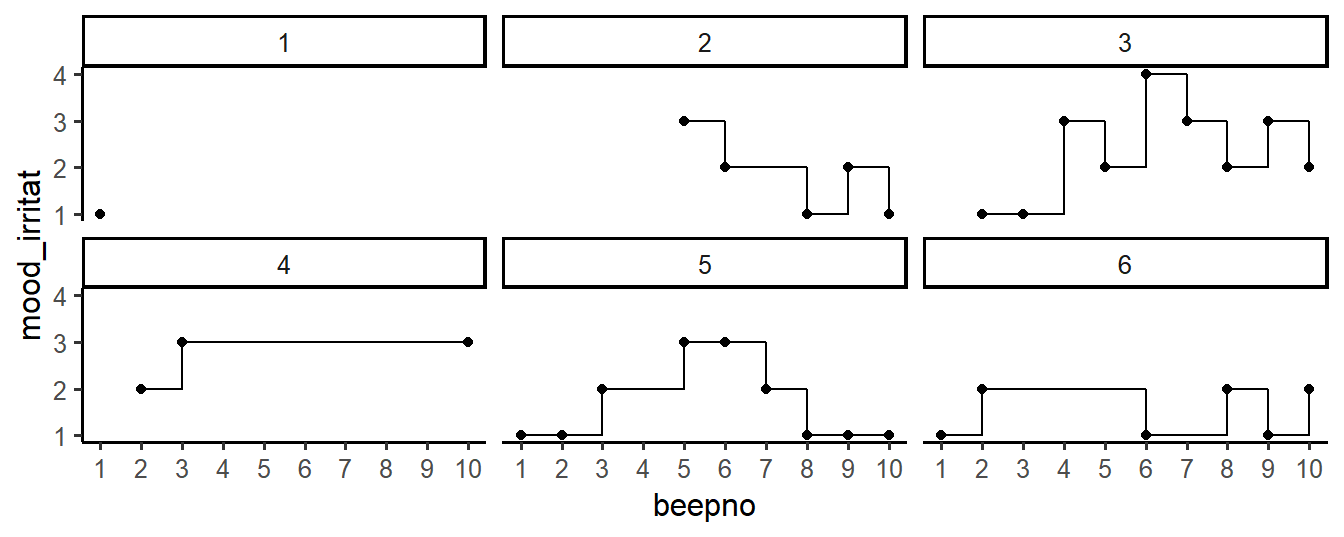
\includegraphics[width=1\linewidth]{R_files/figure-latex/r-irriplot-1} 

}

\caption{Irritation levels of a single patient, in the first six days of an EMA study. Missing values were most prominent at day 1, and irritation varied most at day 3.}\label{fig:r-irriplot}
\end{figure}

\section{Getting Help}\label{getting-help}

\index{R and RStudio!Help}

R has no point-and-click menu's that you can browse through to select a
statistical procedure. This is a problem for many new users. What if you
want, for example, to generate random numbers from a distribution with a
mean of 2 and standard deviation of 4? How to tell this to R?

\subsection{\texorpdfstring{Using `?' to Consult the
Documentation}{Using ? to Consult the Documentation}}\label{using-to-consult-the-documentation}

The good thing is that you already know the name of the function to use,
since we used it in the previous section: it is \texttt{rnorm}. To check
the documentation of this function, type \texttt{?rnorm} in the console.

\begin{Shaded}
\begin{Highlighting}[]
\CommentTok{# Use '?' to find the documentation of a function.}
\NormalTok{?rnorm}
\end{Highlighting}
\end{Shaded}

This opens the documentation of the \texttt{rnorm} function in the
\texttt{Help}-tab, in the bottom right pane, from which you learn that
that the \texttt{rnorm} function accepts \texttt{mean} and \texttt{sd}
(standard deviation) as additional parameters, which are 0 and 1
default, respectively (which explains why \texttt{rnorm(100)} worked in
the previous examples). So, to generate the required numbers, you type:

\begin{Shaded}
\begin{Highlighting}[]
\CommentTok{# Plot the histogram of a custom random sample.}
\KeywordTok{hist}\NormalTok{(}\KeywordTok{rnorm}\NormalTok{(}\DecValTok{1000}\NormalTok{, }\DataTypeTok{mean =} \DecValTok{2}\NormalTok{, }\DataTypeTok{sd =} \DecValTok{4}\NormalTok{))}
\end{Highlighting}
\end{Shaded}

All functions in R are documented, and this documentation is shown in
RStudio's Help pane when you prepend \texttt{?} to the name of the
function in the console.

\subsection{Using RStudio's Global Documentation Index
Search}\label{using-rstudios-global-documentation-index-search}

What if you do not know the name of a function? Suppose you want to run
a t-test for independent groups. Does R have a function for that?

At the top-right of the \texttt{Help} pane, RStudio has a search input
field, which allows you to search through all documentation that is
installed on your computer. The search field auto-completes your input.
If you type a `t' in this field, you will be presented with a list of
functions starting with a `t'. In this list, you find a likely
candidate: a function called \texttt{t.test}. From the documentation of
this function (\texttt{?t.test}), you learn that, indeed, this is the
function you were looking for.

\begin{Shaded}
\begin{Highlighting}[]
\CommentTok{# Run a t-test, on two simulated samples.}

\CommentTok{# generate two samples (N = 100 per group) from the normal distribution}
\NormalTok{A <-}\StringTok{ }\KeywordTok{rnorm}\NormalTok{(}\DecValTok{100}\NormalTok{); B <-}\StringTok{ }\KeywordTok{rnorm}\NormalTok{(}\DecValTok{100}\NormalTok{)}

\CommentTok{# the t-test should be non-significant }
\KeywordTok{t.test}\NormalTok{(A, B)}
\CommentTok{#> }
\CommentTok{#>  Welch Two Sample t-test}
\CommentTok{#> }
\CommentTok{#> data:  A and B}
\CommentTok{#> t = -0.22317, df = 198, p-value = 0.8236}
\CommentTok{#> alternative hypothesis: true difference in means is not equal to 0}
\CommentTok{#> 95 percent confidence interval:}
\CommentTok{#>  -0.3073181  0.2448314}
\CommentTok{#> sample estimates:}
\CommentTok{#>    mean of x    mean of y }
\CommentTok{#> 0.0005615944 0.0318049394}
\end{Highlighting}
\end{Shaded}

\subsection{Learning from Examples}\label{learning-from-examples}

This book contains many R code snippets. By studying these examples, you
will become more familiar with R.

Some examples will introduce R language constructs and functions that
are unknown to you. Learn from these examples, by using \texttt{?} on
each element that you do not understand.

\subsection{Google}\label{google}

With Google, you will find many answers to your R questions. Googling
for ``t-test R'', for example, results in a rich set of online
resources. Good resources are:

\begin{itemize}
\item
  RSeek (see \url{http://rseek.org/})
\item
  Stackoverflow: (see
  \url{https://stackoverflow.com/questions/tagged/r})
\item
  SearchR (see: \url{http://search.r-project.org/})
\end{itemize}

\subsection{Read Books}\label{read-books}

This book does not provide a comprehensive tutorial. There is no need
for that, since excellent resources are readily available. A selection
is presented below.

\begin{itemize}
\item
  Many mental health researchers own a copy of Andy Field's popular book
  ``Discovering Statistics Using IBM SPSS Statistics''
  \citep{FieldSPSS}. For those, Field's R-version of this book,
  ``Discovering Statistics Using R'' \citep{FieldR} provides a familiar
  companion in making the transition to R. See
  \url{https://www.discoveringstatistics.com/}
\item
  Free manuals can be found at the official CRAN site. The manuals are
  dry, but complete and authoritative, since the authors are members of
  the R core development team. See
  \url{https://cran.r-project.org/manuals.html} (or type
  \texttt{help.start()} in the console).
\item
  While at CRAN, be sure to browse the `contributed
  documentation'-section. On this page, you will find many freely
  available manuals contributed by the R community. See
  \url{https://cran.r-project.org/other-docs.html}
\end{itemize}

\subsection{Online Courses}\label{online-courses}

\begin{itemize}
\item
  DataCamp, an online data science education platform, offers several
  interactive courses in R. See \url{http://www.datacamp.com}
\item
  The Try-R course at the CodeSchool website provides an alternative to
  DataCamp. See: \url{http://tryr.codeschool.com/}
\item
  The Quick-R website provides a concise introduction to R. See
  \url{https://www.statmethods.net/}
\end{itemize}

\subsection{Learn R, in R}\label{learn-r-in-r}

\index{swirl}

Package \texttt{swirl} contains a set of interactive courses that teach
many aspects of the R language. See \url{http://swirlstats.com}

\begin{Shaded}
\begin{Highlighting}[]
\CommentTok{# Start the interactive swirl-course.}
\KeywordTok{install.packages}\NormalTok{(}\StringTok{"swirl"}\NormalTok{)}
\KeywordTok{library}\NormalTok{(}\StringTok{"swirl"}\NormalTok{)}
\KeywordTok{swirl}\NormalTok{()}
\end{Highlighting}
\end{Shaded}

\part{EMA Methods}\label{part-ema-methods}

\chapter{Study Design}\label{methods}

\index{Methods} \index{Methods!Study design}

As with all scientific research, EMA studies start with mindful
consideration of the study design. Issues that need to be considered are
the research question(s), the hypotheses, the population of interest,
and the nature of the comparison groups \citep{Shiffman2008}.

Ample information on general study design issues can be found elsewhere
(see for example, the APH quality handbook, at
\url{http://www.emgo.nl/kc/}). This chapter highlights key design
aspects of EMA studies.

\section{What is the EMA Research
Question?}\label{what-is-the-ema-research-question}

Given the plethora of new research options that emerged from the rapid
development in EMA technologies, it can be tempting to dive straight
into exploratory data collection, without giving much consideration to
the theoretical background of the study. That, however, would be one
pitfall of EMA research to avoid. Data mining is no substitute for
theory. Asking participants to contribute data without a rationale is
unethical. As in all scientific activities, defining the research
question should be the first step.

Ask yourself what EMA could bring to your topic of interest. How is it
different from traditional assessment methods? What questions does it
allow you to address that you could not answer without it? For this, you
could use any of the EMA advantages discussed in Chapter
\ref{introduction}. Are you interested in real-life behavior, in
differences between participants, in changes within participants over
time, or in potential causal pathways between health-related variables?
What relationships do you expect to find, and why? A solid theoretical
background, and clearly formulated explicit research questions and
hypotheses will help to make the right choices when you have to decide
on the other aspects of the study design.

\section{Who are the Study
Participants?}\label{who-are-the-study-participants}

Given the experimental nature of EMA, studies are often piloted in
healthy or sub-clinical populations. This is a recommended first step,
to test the experimental procedures and to avoid unnecessary burdening
of vulnerable patient populations. You should be aware, though, that
results obtained in non-patient populations do not necessarily
generalize to patient populations. EMA mood ratings, for example, might
be much more variable in patients compared to non-patients. Pilot
studies should therefore also be conducted in the target population. It
is also advisable to write a manual on how to operate the EMA device and
spend time on briefing participants on what is expected of them during
the study. Depending on your study topic and EMA method, de-briefing
might also be nescesarry, along with instructions on how to return a
wearable or de-install an EMA app.

\section{What are the Qualities of the EMA
Measures?}\label{what-are-the-qualities-of-the-ema-measures}

\index{EMA!Passive EMA} \index{EMA!Active EMA} \index{Measurement error}

With the study hypotheses in place, theoretical constructs must be
operationalized into quantitative measures. For this, you should consult
the scientific literature on the reliability and validity of existing
EMA measures \citep[e.g.,][]{Moore2016, Rijsbergen2012}.

In active EMA research, complex multi-dimensional constructs such as
mood and anxiety are often measured using single-item questions, to
reduce the assessment burden of participants, who are prompted several
times per day. You should ask yourself (and the scientific literature)
what the psychometric properties are of these measures. How do these
EMA-measures compare to scores on traditional assessments (e.g.,
self-report questionnaires, clinical interviews)? What is known about
the variability of items scores? And what is known about the measurement
errors? Surprisingly, these last questions are often ignored in EMA
research, even though it has been estimated that up to 30\% to 50\% of
the observed variance in intensive repeated measures data can be
attributable to measurement error \citep{Schuurman2015}.

In passive EMA research, it is important to be aware of the
characteristics and limitations of the `data acquisition interfaces'
\citep{Stone2002}. For example, if you want to collect accelerometer
data, a variety of options exist. You can collect these data via the
built-in accelerometer of the smartphone of the participants, via cheap
commercially available activity trackers, such as Fitbit, or via
expensive wearable devices that are developed specifically for
scientific research. Each option comes with specific advantages and
disadvantages. Smartphone-based accelerometer data, for example, can be
collected with relative ease, but these data can also be noisy and
incomplete, since samples rates can often not be set and the precision
of the built-in sensors varies considerably from device to device.
Commercial accelerometers may have better precision and reliability
\citep[see, e.g.,][]{Evenson2015}, but manufacturers often limit access
to raw data and data pre-processing algorithms, making it difficult (or
even impossible) to fully analyze outcomes.`Scientific wearables' do
offer this access, but often choose function over form (design). They
can therefore draw attention, prompting unwanted questions to
partcipants. Being aware of these issues when you plan the study, will
help considerably in the analysis stage of your study.

\section{What is the Sample Plan?}\label{what-is-the-sample-plan}

\index{Sampling}

An important next step is to define the EMA data sample plan. Questions
that need to be answered are:

\begin{itemize}
\tightlist
\item
  How many days will data collection last?
\item
  On each day, how often are participants assessed?
\item
  How and when are participants invited for assessment?
\end{itemize}

The questions above should be answered as detailed as possible to best
serve the research question and the statistical power (see below). In
practice, however, it is often necessary to balance research interests,
respondent burden, and practical considerations, such as hardware
limitations.

When determining the appropriate sample plan, start with mapping the
expected fluctuation or patterns, based on available knowledge. For
example, when an event is rare, it can be sufficient to ask participants
to initiate EMA whenever the event occurs, or prompt them with an
end-of-day diary. Adding more prompts in this scenario would not lead to
more reliable data \citep{Piasecki2007}. Increasing the assessment
frequency and study duration will allow for a more detailed assessment
of the outcome of interest. It is tempting to collect often and for a
long period of time. However, this may also increase respondent burden,
which may, in turn, affect study adherence and accuracy. Measurement
reactivity could also occur, where the EMA-induced enhanced focus on the
outcome of interest causes participants to increase or decrease on this
outcome \citep{Hufford2002, VanBallegooijen2016}.

Issues related to hardware should also be considered. Electronic
wearables have limited battery life and memory storage space. Memory
space limitations of actigraphy watches may require participants to
visit the research site. GPS-monitoring apps may have a negative impact
on the battery life of the smartphone of the participants. These
practical issues may also result in data loss and study drop-out.

Once all decisions related to the sampling plan are made, the procedure
should be thoroughly tested. As a first step, it can be insightful to
simulate the sample plan, as is done below, using the
\texttt{sample\_plan} function, which is part of package \texttt{emaph}:

\begin{Shaded}
\begin{Highlighting}[]
\CommentTok{# Simulating a signal-contingent sample plan.}
\KeywordTok{library}\NormalTok{(emaph)}
\NormalTok{plan <-}\StringTok{ }\KeywordTok{sample_plan}\NormalTok{(}\DataTypeTok{n_participants =} \DecValTok{5}\NormalTok{,}
                    \DataTypeTok{n_days =} \DecValTok{2}\NormalTok{,}
                    \DataTypeTok{times =} \KeywordTok{c}\NormalTok{(}\StringTok{"09:00-11:00"}\NormalTok{, }\StringTok{"12:30"}\NormalTok{, }\StringTok{"17:00-19:00"}\NormalTok{),}
                    \DataTypeTok{plot =} \OtherTok{TRUE}\NormalTok{)}
\end{Highlighting}
\end{Shaded}

\begin{figure}

{\centering 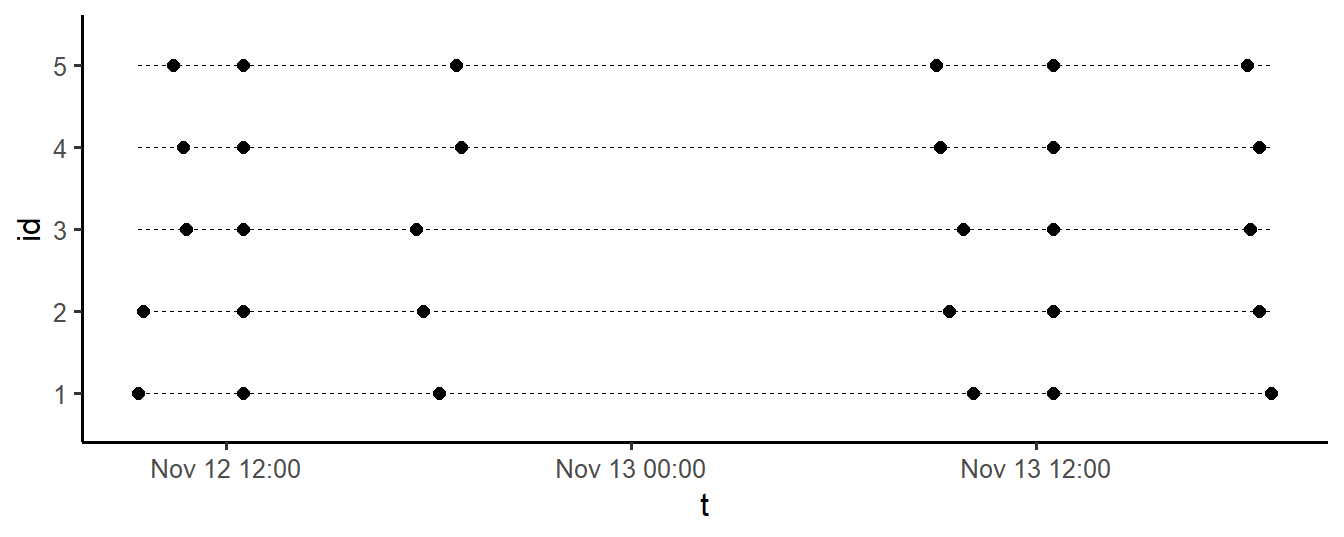
\includegraphics[width=0.95\linewidth]{study-design_files/figure-latex/fig3a-1} 

}

\caption{Generated two-day EMA sampling plan, for 5 participants}\label{fig:fig3a}
\end{figure}

\section{What is the Optimal Sample
Size?}\label{what-is-the-optimal-sample-size}

\index{Methods!Power analysis} \index{pwr}

The power of a statistical test is the probability that it will detect
an effect when this effect, in reality, exists. It is a function of the
strength of the effect size, sample size, the significance level
(alpha), \emph{and} the statistical model. Determining the power of the
experiment is an important step in the design of any study - EMA studies
included. Both under-powered and overpowered studies are a waste of time
and resources.

Conducting a power analysis can be easy or very difficult, depending on
the complexity of the experimental design and the adopted statistical
technique. For simple tests, such as the t-test and ANOVA,
straightforward analytic solutions exist, which are implemented in
readily available tools. In R, one of those tools is package
\texttt{pwr} (which you can install, as you now know, via
\texttt{install.packages(\textquotesingle{}pwr\textquotesingle{})}).

For example, to use \texttt{pwr} to calculate the power of a t-test to
detect a moderate effect size (\emph{d} = 0.5), with n = 30 per group,
and a (two-sided) significance level alpha of .05, type:

\begin{Shaded}
\begin{Highlighting}[]
\CommentTok{# Power analysis of a t-test}
\CommentTok{# (analytical approach).}

\KeywordTok{library}\NormalTok{(pwr)}
\KeywordTok{pwr.t.test}\NormalTok{(}\DataTypeTok{d =} \FloatTok{0.5}\NormalTok{, }
           \DataTypeTok{n =} \DecValTok{30}\NormalTok{,}
           \DataTypeTok{sig.level =} \FloatTok{0.05}\NormalTok{,}
           \DataTypeTok{type =} \StringTok{"two.sample"}\NormalTok{,}
           \DataTypeTok{alternative =} \StringTok{"two.sided"}\NormalTok{)}
\CommentTok{#> }
\CommentTok{#>      Two-sample t test power calculation }
\CommentTok{#> }
\CommentTok{#>               n = 30}
\CommentTok{#>               d = 0.5}
\CommentTok{#>       sig.level = 0.05}
\CommentTok{#>           power = 0.4778965}
\CommentTok{#>     alternative = two.sided}
\CommentTok{#> }
\CommentTok{#> }\AlertTok{NOTE}\CommentTok{: n is number in *each* group}
\end{Highlighting}
\end{Shaded}

The power is 48\% - not even close to the generally adopted standard of
80\%. More participants are needed to detect the hypothesized effect.
Can you find the \texttt{n} for which power is 80\%?

EMA study designs are often characterized by repeated measures, complex
multi-level structures and the application of advanced statistical
techniques. You may find that available power calculators are too
limited to properly take key aspects of your design into account. If
this happens, simulation techniques may help. If power is the
probability that a test will detect an effect it is exists, it can be
determined by noting the proportion of times a statistical test reaches
significance, if it is run, many times, on simulated data, in which the
hypothesized effect is present. To illustrate how this works, we will
calculate the power of the t-test again, through simulation:

\index{Simulating data} \index{MASS} \index{simstudy}

\begin{Shaded}
\begin{Highlighting}[]
\CommentTok{# Power analysis of a t-test}
\CommentTok{# (simulation approach).}

\NormalTok{m1 =}\StringTok{ }\DecValTok{0}   \CommentTok{# mean in group 1  }
\NormalTok{m2 =}\StringTok{ }\FloatTok{0.5} \CommentTok{# mean in group 2}
\NormalTok{sd =}\StringTok{ }\DecValTok{1}   \CommentTok{# sd (in both groups)}
\NormalTok{n =}\StringTok{ }\DecValTok{30}   \CommentTok{# sample size, per group}

\CommentTok{# conduct the experiment many times}
\NormalTok{nsim <-}\StringTok{ }\DecValTok{10000}
\NormalTok{p <-}\StringTok{ }\KeywordTok{numeric}\NormalTok{(nsim)}
\ControlFlowTok{for}\NormalTok{ (i }\ControlFlowTok{in} \DecValTok{1}\OperatorTok{:}\NormalTok{nsim) \{}
  
\NormalTok{  data <-}\StringTok{ }\KeywordTok{data.frame}\NormalTok{(}
\NormalTok{    outcome <-}\StringTok{ }\KeywordTok{c}\NormalTok{(}
      \KeywordTok{rnorm}\NormalTok{(n, m1, sd), }\CommentTok{# group 1 data}
      \KeywordTok{rnorm}\NormalTok{(n, m2, sd)  }\CommentTok{# group 2 data}
\NormalTok{    ),}
\NormalTok{    group <-}\StringTok{ }\KeywordTok{c}\NormalTok{(}
      \KeywordTok{rep}\NormalTok{(}\DecValTok{1}\NormalTok{, n), }\CommentTok{# group 1 indicator}
      \KeywordTok{rep}\NormalTok{(}\DecValTok{2}\NormalTok{, n)) }\CommentTok{# group 2 indicator}
\NormalTok{  )}
  
  \CommentTok{# save significance of test}
\NormalTok{  p[i] <-}\StringTok{ }\KeywordTok{t.test}\NormalTok{(outcome }\OperatorTok{~}\StringTok{ }\NormalTok{group, data)}\OperatorTok{$}\NormalTok{p.value}
\NormalTok{\}}

\CommentTok{# power}
\KeywordTok{sum}\NormalTok{(p }\OperatorTok{<}\StringTok{ }\FloatTok{0.05}\NormalTok{) }\OperatorTok{/}\StringTok{ }\NormalTok{nsim}
\CommentTok{#> [1] 0.4753}
\end{Highlighting}
\end{Shaded}

As can be seen, the simulation results are very close to the output of
\texttt{pwr.t.test}. There was no immediate need to run this simulation.
We already knew that the power was 48\%. The example illustrates,
however, that simulation is a valid option when power calculators are
too limited. Simulating the right data, of course, can be challenging as
well, but you will find that R has packages that simplify data
simulation. For example, \texttt{mvrnorm} in package \texttt{MASS}
\citep{Venables2002} can be used to generate correlated data, and
package \texttt{simstudy} \citep{R-simstudy} can be used to generate
complex longitudinal and hierarchical data.

\section{What are the Ethical
Aspects?}\label{what-are-the-ethical-aspects}

\index{Methods!Ethical considerations}

All clinical studies that involve human participants need to be
evaluated by a Medical Research and Ethics Committee (MREC; Dutch:
`METC'). Recently, the committees have also been tasked to determine
whether a medical device is used and to evaluate the safety and quality
of the device. Researchers are therefore required to add a section in
the research protocol, explaining why the software/device is or is not a
medical device. The official definition of a medical device (Medical
Device Act, or `Wet Medische Hulpmiddelen') is as follows:

\begin{quote}
``Any instrument, apparatus or appliance, any software or material or
any other article that is used alone or in combination, including any
accessory and the software required for its proper operation, that is
intended by the manufacturer to be used specifically for diagnostic or
therapeutic purposes, and is intended by the manufacturer to be used for
human beings for the purpose of: - diagnosis, prevention, monitoring,
treatment or alleviation of disease - diagnosis, monitoring, treatment,
alleviation of or compensation for an injury or handicap -
investigation, replacement or modification of the anatomy or of a
physiological process - control of conception, and which does not
achieve its principal intended action in or on the human body by
pharmacological, immunological or metabolic means, but which may be
assisted in its function by such means.'' \citep{ccmo_meddev}
\end{quote}

In short, software can be classified as a medical device when it
collects patient-specific data and when it is specifically intended for
one of the above-mentioned objectives. In practice, the definition of
medical devices leaves a lot of room for confusion. Researchers often
struggle with the question whether their assessment tools should be
considered a medical device or not. For this purpose, flowcharts exist
that help to determine whether an app or another software product should
be classified as a medical device \citep[see, e.g.,][and
\url{http://cetool.nl/general/scanAid}]{Ekker2013}. Figure
\ref{fig:fig3b} shows such a flow-chart.

While planning your EMA study, you should also be mindful of the rules
and regulations that apply to data collection, storage and sharing. From
May 2018 onward, the European Committee has enforced the General Data
Protection Regulation (GDPR; in Dutch: ``Algemene Verordening
Gegevensbescherming - AVG''``; see \url{https://gdpr-info.eu/}), which
protects the data and privacy of EU citizens. Complying to the GDPR can
be a complex and time-consuming process, depending on nature of your
study. Do not hesitate to consult local experts or standard guidelines
provided by your organization (see, e.g.,
\url{http://www.emgo.nl/kc/checklist-avg/}).

In EMA studies, an important GDPR-related issue concerns the Data
Processing Agreement (DPA). When data processing is (partly) outsourced
to a third party, a Data Processing Agreement (DPA) should be drafted,
that specifies the agreements between the `controller' and `processor'.
In this context, a controller is the person or organization that
determines the why and how of data collection (for example you as a
researcher). The processor processes the data on behalf of the
controller, for example by providing a data-collection service, or by
storing raw study data on a cloud-server.

Aspects of data processing that need to be addressed in this agreement
include the context, duration and termination of agreement, the nature
of the data collected, the duration of data storage, security measures
taken to prevent unauthorized access, and agreements on data ownership,
data sharing, the handling of personal data breaches, and liability.
Most organizations offer model agreements in which all relevant issues
are addressed. Third parties may offer model agreements as well. If so,
however, these agreements need to be checked for compliance to local
regulations.

\begin{figure}

{\centering 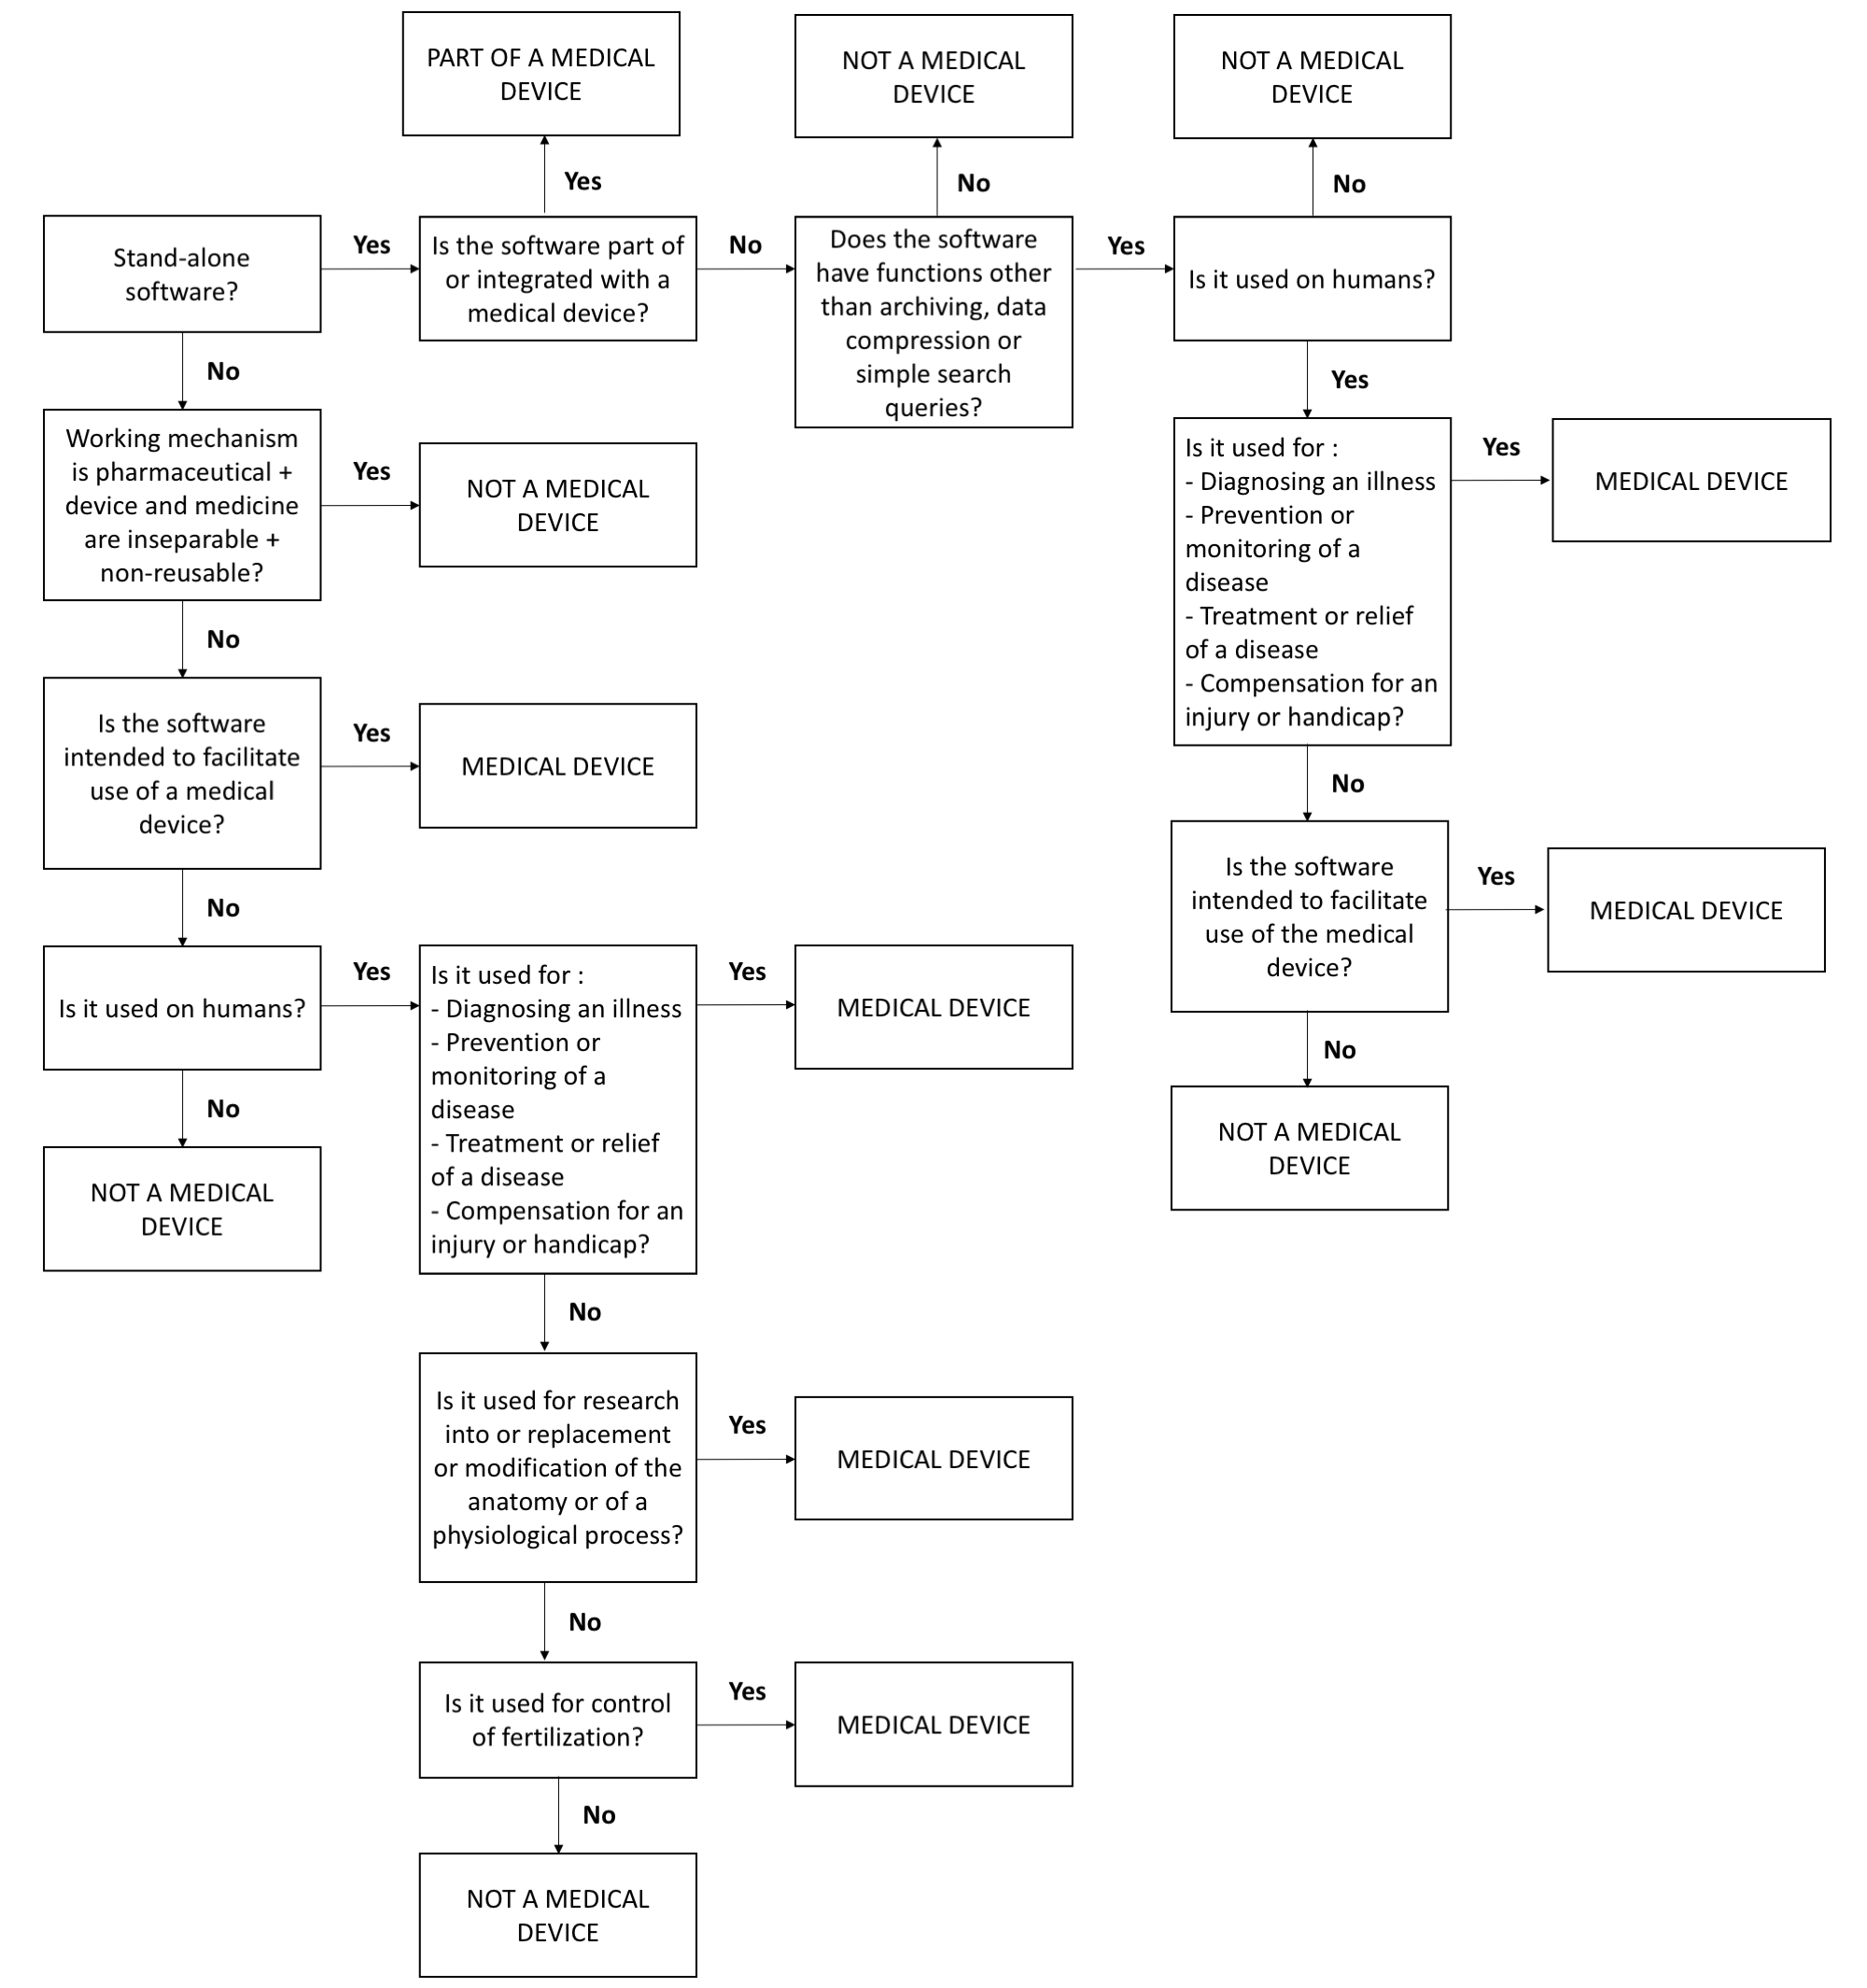
\includegraphics[width=0.9\linewidth]{images/outcomes/Medical_deviceFC} 

}

\caption{Flow-chart to determine whether study devices (including EMA apps) should be considered a medical device. Based on http://cetool.nl/general/scanAid}\label{fig:fig3b}
\end{figure}

\chapter{Data Management}\label{datamanagement}

\index{Datamanagement}

In a typical EMA study, lots of data are collected. Repeated
self-reports, GPS-data, accelerometer data, background demographic data
and traditional questionnaire data quickly add up to gigabytes of raw
data. Without proper data management, the EMA researcher would drown in
these data. Fortunately, R and RStudio are useful aids to prevent this
from happening. R is very flexible in the management of multiple data
files, and RStudio includes a handy feature, called ``Projects'', with
which data and analysis scripts can be stored in an orderly fashion.

\section{Using RStudio-projects}\label{using-rstudio-projects}

\index{RStudio Projects}

RStudio projects can be opened by double-clicking existing projects, or
by creating new projects from RStudio's file menu. To create a new
project, choose \texttt{File\ \textgreater{}\ New\ Project...}. You will
be asked to specify the project name and its disk location (as shown in
\ref{fig:fig5a}, after which the project will open in a new window.

\begin{figure}

{\centering 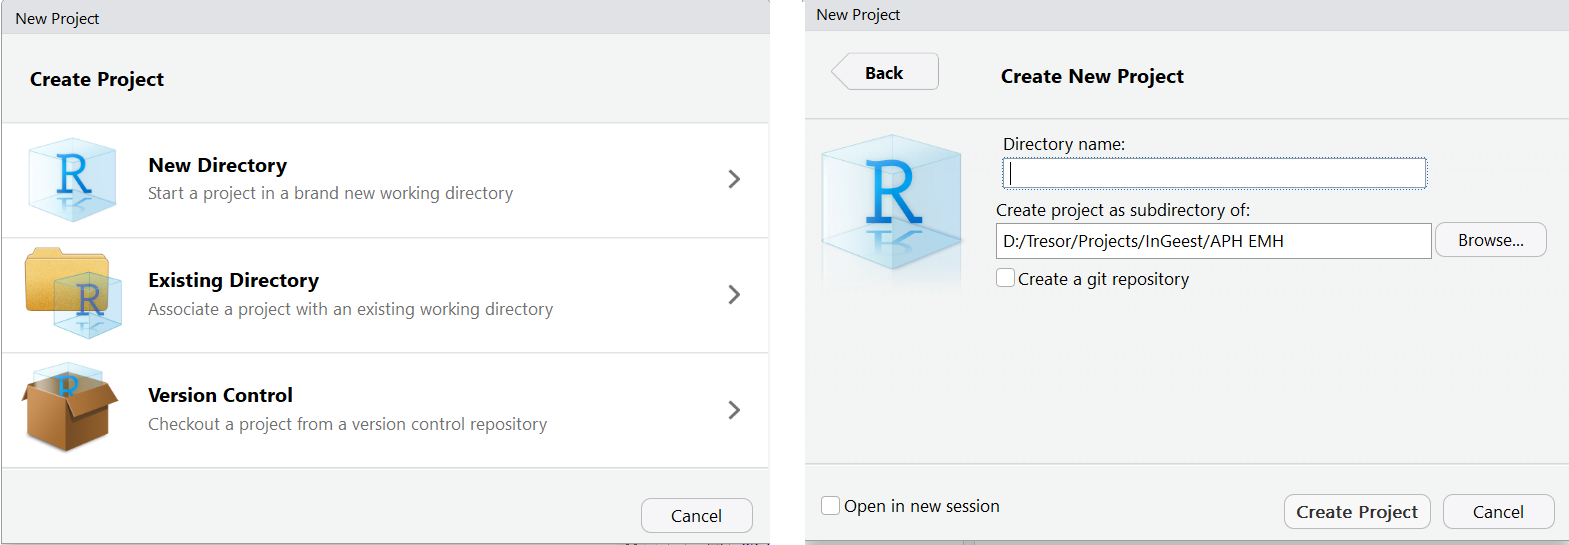
\includegraphics[width=0.7\linewidth]{images/datamanagement/new_project} 

}

\caption{creating a project in RStudio}\label{fig:fig5a}
\end{figure}

One of the advantages of using RStudio Projects is that projects set the
working directory to the project directory location. You can verify this
by asking R to print the current working directory, by typing the
\texttt{getwd()} function in the console, while the project is open.

This may look like a trivial feature. It is, however, a great advantage,
because it allows for the use of relative paths, which is very
convenient. For example, to open a data source in a script, you no
longer have to specify its full path (e.g.,
`D:/work/projects/my\_ema\_project/data/raw/ema\_data.csv'). With
relative paths, you can simply type `data/raw/ema\_data.csv'. This saves
typing, but, more importantly, it allows you to freely move your
projects to other locations, without breaking the proper functioning of
your scripts.

\section{An Example Project Directory
Structure}\label{an-example-project-directory-structure}

\index{Datamanagement!Project directory structure}

RStudio imposes no limitations to the contents of project directories.
You are free to organize the project in the way you want. In clinical
research, however, you are advised to choose a structure that aids you
best to implement the following research guidelines:

\begin{itemize}
\item
  You should adhere strictly to a clear and logical directory structure,
  to ensure that co-workers and external auditors can quickly grasp and
  replicate your work;
\item
  Raw data should be part of your project, so that results can be traced
  back to their source;
\item
  Cleaned data should be separated from raw data, and data cleaning
  procedures should be explicit and replicable;
\item
  Data and analyses should be clearly separated;
\item
  All analyses should be explicit and replicable;
\item
  Output of (published) analyses should be saved.
\end{itemize}

A directory structure based on these guidelines is listed in Figure
\ref{fig:dm-project-tree}. It shows the organization of a (hypothetical)
project in which data were collected via:

\begin{enumerate}
\def\labelenumi{\arabic{enumi}.}
\item
  an online survey system, to assess demographics and pre/post study
  depression severity (with the PHQ-9 questionnaire,
  \citet{Kroenke2009}),
\item
  an active EMA smartphone app, to assess day-to-day changes in mood,
  and
\item
  an accelerometer to assess activity levels.
\end{enumerate}

\begin{figure}

{\centering 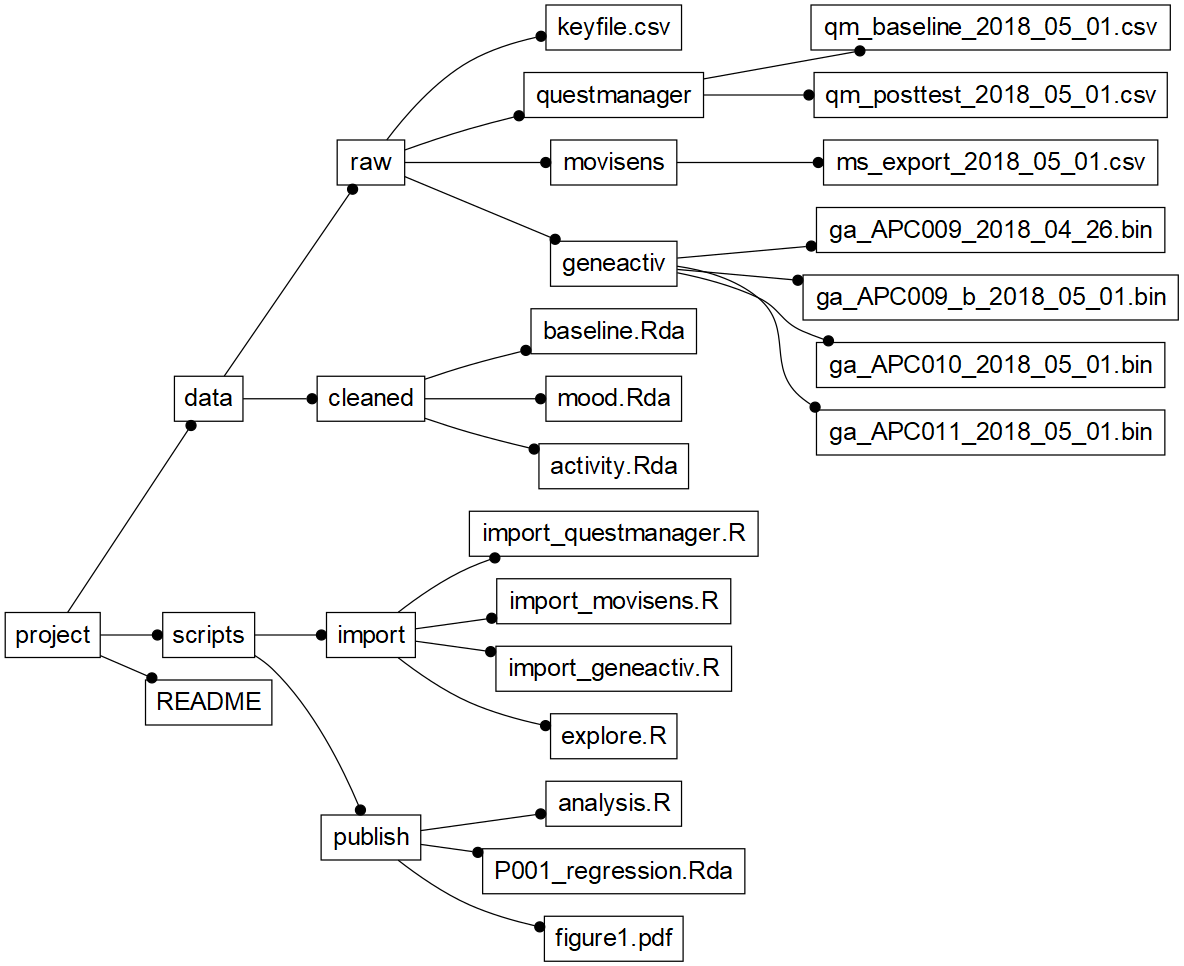
\includegraphics[width=0.65\linewidth]{images/datamanagement/project_tree} 

}

\caption{Example project directory structure}\label{fig:dm-project-tree}
\end{figure}

\section{Data}\label{data}

\index{Datamanagement!Raw data}

Full replicability implies that raw data can be traced back to the
source. Wherever possible, this should translate to the availability of
raw study data in your project.

In the example project, unprocessed data files exported from the three
data collection systems (i.e., survey data, EMA data, and actigraphy
data) are stored in the 'data/raw``-directory', in separate
sub-directories per data type.

In `data/raw/survey', we find two files: 1) `sur\_t0\_2018\_05\_01.csv',
containing the results of demographic questionnaire and the PHQ-9
pre-test, and 2) and `sur\_t1\_2018\_05\_01.csv', containing the results
of the PHQ-9 post-test. In exports of such survey systems, data from all
participants are typically stored in one file per assessment moment.
Note how the export date is added to the files, to make sure that future
updates are only used in the analysis when explicitly noted.

In `data/raw/ema', we find one file: `ema\_2018\_05\_01.csv', containing
the results of the EMA mood measurements of all participants, exported
from the back-office of the EMA platform.

Finally, in `data/raw/actigraphy', we see a series of `.bin' files:
binary data files that were exported from, e.g., GENEActiv smart
watches, that were worn by the participants. Actigraphy data are
high-volume data: these files are typically large (500MB is no
exception). By using the `.bin' format, in which data are compressed,
disk space is saved (in uncompressed format, data in a single .bin file
can amount up to 2 GB). Unlike the survey and EMA mood data, each data
file in this directory contains data of one participant. In this case,
there are even two files for one participant (`APC009'), perhaps because
this participant started the study with a faulty device, which was
swapped during the study.

In `data/raw', a final very important file is `key\_file.csv'. This file
is important because it ties all the data together. It contains the
unique identifiers (IDs) that are assigned to the study participants in
the various data collection systems. Ideally, of course, participants
would be designated by a single ID in each data collection system. In
practice, unfortunately, this is often not possible due to limitations
of the systems used. As a result, researchers are forced to deal with
the fact that participants are known under different IDs in each system.
With a key-file, data can be tied together through scripts.

In the example key-file below, we find four columns. The first column
defines the global study ID for each participant (i.e., the ID that the
researcher intends to use as the ``official'' ID). The other three
columns define how the participant is identified in each data collection
system.

\begin{longtable}[]{@{}llll@{}}
\caption{\label{tab:tab5a} Example Study Key-file}\tabularnewline
\toprule
ID & Survey\_ID & EMA\_ID & Actigraphy\_ID\tabularnewline
\midrule
\endfirsthead
\toprule
ID & Survey\_ID & EMA\_ID & Actigraphy\_ID\tabularnewline
\midrule
\endhead
P001 & QM01221 & 192.A102.83A & APC009\tabularnewline
P002 & QM01228 & 192.B106.73X & APC010\tabularnewline
P003 & QM01230 & 192.B220.00N & APC011\tabularnewline
\bottomrule
\end{longtable}

\section{Import Scripts}\label{import-scripts}

\section{Cleaning}\label{cleaning}

In `scripts/import', we find the scripts with which the raw data are
imported and cleaned, to produce ready-to-analyze data that are stored
in `data/cleaned'.

By making these scripts parts of your project, you ensure that you and
others can always trace the decisions that were made to prepare the raw
data for analysis. Raw data may be updated, for instance because more
participants are recruited, or because new data exports are made from
the data collection systems. You may also detect errors in the import
routines during the analyses, or peer reviewers may request information
that can only be found by going back to the raw data. In all these
cases, the availability of ready-to-run raw data import routines is
crucial.

The code snippet below illustrates the kind of data transformations that
you can expect to find in an import script. With a few lines of code,
raw baseline questionnaire data are imported into R, participant id's
that are specific to the data collection system are replaced by the
proper global study id, variables of interest are selected, data ranges
are checked (and corrected if needed), and data types are set (in
accordance to the study code-book). Finally, the cleaned data set is
saved to the `data/cleaned' folder, ready for further processing in the
final analyses.

\begin{Shaded}
\begin{Highlighting}[]
\CommentTok{# ------------------------------------------------------------}
\CommentTok{# Clean data }
\CommentTok{# JR - 2018-10-16}
\CommentTok{# ------------------------------------------------------------}

\CommentTok{# import raw baseline survey data (csv file) -----------------}
\NormalTok{t0 <-}\StringTok{ }\KeywordTok{read.csv}\NormalTok{(}\StringTok{"data/raw/survey/sur_t0_2018_05_01.csv"}\NormalTok{)}

\CommentTok{# inject study ID, from study key file -----------------------}
\NormalTok{keys <-}\StringTok{ }\KeywordTok{read.csv}\NormalTok{(}\StringTok{"data/raw/keyfile.csv"}\NormalTok{)}
\NormalTok{t0 <-}\StringTok{ }\KeywordTok{merge}\NormalTok{(t0, keys)}

\CommentTok{# only keep variables of interest ----------------------------}
\CommentTok{# (gender, age, phq item scores)}
\NormalTok{t0 <-}\StringTok{ }\NormalTok{t0[}\KeywordTok{c}\NormalTok{(}\StringTok{"ID"}\NormalTok{, }\StringTok{"gender"}\NormalTok{, }\StringTok{"age"}\NormalTok{, }\KeywordTok{paste0}\NormalTok{(}\StringTok{"phq"}\NormalTok{, }\DecValTok{1}\OperatorTok{:}\DecValTok{9}\NormalTok{)]}

\CommentTok{# turn gender into a proper factor ---------------------------}
\NormalTok{t0}\OperatorTok{$}\NormalTok{gender <-}\StringTok{ }\KeywordTok{factor}\NormalTok{(t0}\OperatorTok{$}\NormalTok{gender, }\DataTypeTok{levels =} \KeywordTok{c}\NormalTok{(}\StringTok{"M"}\NormalTok{, }\StringTok{"F"}\NormalTok{))}

\CommentTok{# replace out-of-range data with missing values (NA) ---------}
\NormalTok{t0}\OperatorTok{$}\NormalTok{age[t0}\OperatorTok{$}\NormalTok{age }\OperatorTok{>}\StringTok{ }\DecValTok{100}\NormalTok{] <-}\StringTok{ }\OtherTok{NA}
\NormalTok{t0}\OperatorTok{$}\NormalTok{age[t0}\OperatorTok{$}\NormalTok{age }\OperatorTok{<}\StringTok{ }\DecValTok{5}\NormalTok{] <-}\StringTok{ }\OtherTok{NA}

\CommentTok{# replace out-of-range phq item data with missing values -----}
\NormalTok{t0[}\KeywordTok{paste0}\NormalTok{(}\StringTok{"phq"}\NormalTok{, }\DecValTok{1}\OperatorTok{:}\DecValTok{9}\NormalTok{)] <-}\StringTok{ }\KeywordTok{lapply}\NormalTok{(}
\NormalTok{  t0[}\KeywordTok{paste0}\NormalTok{(}\StringTok{"phq"}\NormalTok{, }\DecValTok{1}\OperatorTok{:}\DecValTok{9}\NormalTok{)], }
  \ControlFlowTok{function}\NormalTok{(x) \{}
\NormalTok{    x[x }\OperatorTok{<}\StringTok{ }\DecValTok{0}\NormalTok{] <-}\StringTok{ }\OtherTok{NA}
\NormalTok{    x[x }\OperatorTok{>}\StringTok{ }\DecValTok{3}\NormalTok{] <-}\StringTok{ }\OtherTok{NA}
\NormalTok{  \})}

\CommentTok{# save cleaned baseline data --------------------------------- }
\KeywordTok{save}\NormalTok{(t0, }\DataTypeTok{file =} \StringTok{"data/cleaned/t0.Rda"}\NormalTok{)}
\end{Highlighting}
\end{Shaded}

The code snippet above illustrates the importance of code documentation.
You may struggle to immediately understand some of the code segments.
For instance, you might not be familiar with the \texttt{paste0}
function that is used to create the names of the variables that contain
the PHQ-9 item scores. Fortunately, however, the comment (the lines
starting with \texttt{\#}) make it clear that the function is used to
select individual PHQ-9 items. Comment your code. You will do yourself
and your colleagues a big favor by making it much easier to quickly
grasp the meaning of your code.

\section{Pre-process}\label{pre-process}

Once data are cleaned, you can enrich the data sets with variables that
can be derived from the raw data, such as, e.g., survey scale and
subscale scores, if needed), or actigraphy summary measures (see Chapter
\ref{activity}). The example below calculates the PHQ-9 sum scores from
the item scores in the cleaned baseline data:

\begin{Shaded}
\begin{Highlighting}[]
\CommentTok{# ------------------------------------------------------------}
\CommentTok{# Pre-process data }
\CommentTok{# JR - 2018-10-16}
\CommentTok{# ------------------------------------------------------------}

\CommentTok{# import cleaned baseline survey data ------------------------}
\KeywordTok{load}\NormalTok{(}\StringTok{"data/cleaned/baseline.Rda"}\NormalTok{)}
\KeywordTok{load}\NormalTok{(}\StringTok{"data/cleaned/posttest.Rda"}\NormalTok{)}

\CommentTok{# add PHQ-9 sum scores ---------------------------------------}
\NormalTok{baseline}\OperatorTok{$}\NormalTok{phq9 <-}\StringTok{ }\KeywordTok{rowSums}\NormalTok{(baseline[}\KeywordTok{paste0}\NormalTok{(}\StringTok{"phq"}\NormalTok{, }\DecValTok{1}\OperatorTok{:}\DecValTok{9}\NormalTok{)], }
                         \DataTypeTok{na.rm =} \OtherTok{TRUE}\NormalTok{)}
\NormalTok{posttest}\OperatorTok{$}\NormalTok{phq9 <-}\StringTok{ }\KeywordTok{rowSums}\NormalTok{(posttest[}\KeywordTok{paste0}\NormalTok{(}\StringTok{"phq"}\NormalTok{, }\DecValTok{1}\OperatorTok{:}\DecValTok{9}\NormalTok{)], }
                         \DataTypeTok{na.rm =} \OtherTok{TRUE}\NormalTok{)}

\CommentTok{# re-save baseline data --------------------------------------}
\KeywordTok{save}\NormalTok{(baseline, }\DataTypeTok{file =} \StringTok{"data/cleaned/baseline.Rda"}\NormalTok{)}
\KeywordTok{save}\NormalTok{(baseline, }\DataTypeTok{file =} \StringTok{"data/cleaned/posttest.Rda"}\NormalTok{)}
\end{Highlighting}
\end{Shaded}

\section{Combine}\label{combine}

While working on your project, you will probably want to re-run the
cleaning and pre-processing scripts a lot, for instance in response to
additional data coming in, or to fix bugs in the import routines. For
this, it can be helpful to create one file in which all import scripts
are executed in proper sequence. For this, you can use R's
\texttt{source} command, with which scripts can be read and executed
directly from disk:

\begin{Shaded}
\begin{Highlighting}[]
\CommentTok{# ------------------------------------------------------------}
\CommentTok{# Import (clean & pre-process) all data files }
\CommentTok{# JR - 2018-10-16}
\CommentTok{# ------------------------------------------------------------}

\CommentTok{# clean -------------------------------}
\KeywordTok{source}\NormalTok{(}\StringTok{"scripts/import/clean_surveys.R"}\NormalTok{) }
\KeywordTok{source}\NormalTok{(}\StringTok{"scripts/import/clean_ema.R"}\NormalTok{) }
\KeywordTok{source}\NormalTok{(}\StringTok{"scripts/import/clean_actigraphy.R"}\NormalTok{) }

\CommentTok{# pre-process----------------------------}
\KeywordTok{source}\NormalTok{(}\StringTok{"scripts/import/calc_surveys.R"}\NormalTok{) }
\KeywordTok{source}\NormalTok{(}\StringTok{"scripts/import/calc_ema.R"}\NormalTok{)}
\KeywordTok{source}\NormalTok{(}\StringTok{"scripts/import/calc_actigraphy.R"}\NormalTok{) }
\end{Highlighting}
\end{Shaded}

\section{Reproducible Analyses}\label{reproducible-analyses}

When raw data stored, imported and cleaned, final analyses can be run.
By basing these analyses on the cleaned data in `data/cleaned', you
ensure that these analyses can be fully reproduced from the raw study
data.

The code snippet below illustrates a typical analysis file: cleaned data
are loaded into the R work environment, after which EMA scores of a
single participant are selected, plotted and analyzed in a simple linear
regression. Both the plot and the result of the regression are saved in
the analysis directory. The plot is saved as a PDF-file (ready for
submission to the journal), and the regression results are saved in a
standard R data structure.

\begin{Shaded}
\begin{Highlighting}[]
\CommentTok{# -------------------------------------------------------------}
\CommentTok{# N = 1 Analysis (P001)}
\CommentTok{# note: part of manuscript!}
\CommentTok{# JR - 2018-10-16}
\CommentTok{# ------------------------------------------------------------}

\CommentTok{# import cleaned EMA mood study data --------------------------}
\KeywordTok{load}\NormalTok{(}\StringTok{"data/cleaned/ema.Rda"}\NormalTok{)}

\CommentTok{# create and save Figure 1: EMA mood data, of participant P001 }
\NormalTok{d <-}\StringTok{ }\KeywordTok{subset}\NormalTok{(mood, ID }\OperatorTok{==}\StringTok{ "P001"}\NormalTok{)}
\KeywordTok{pdf}\NormalTok{(}\DataTypeTok{file =} \StringTok{"scripts/published/figure1.pdf"}\NormalTok{)}
\KeywordTok{plot}\NormalTok{(mood }\OperatorTok{~}\StringTok{ }\NormalTok{time, d)}
\KeywordTok{dev.off}\NormalTok{()}

\CommentTok{# run a regression model on P001 mood data}
\NormalTok{fm <-}\StringTok{ }\KeywordTok{lm}\NormalTok{(mood }\OperatorTok{~}\StringTok{ }\NormalTok{time, d)}
\KeywordTok{summary}\NormalTok{(fm)}

\CommentTok{# save regression results }
\KeywordTok{save}\NormalTok{(fm, }\DataTypeTok{file =} \StringTok{"scripts/published/P001_regression.Rda"}\NormalTok{)}
\end{Highlighting}
\end{Shaded}

R's ability to save the results of analyses to disk is yet another
example of how R promotes accountability in clinical research. Suppose
you used the regression analysis of `P001' in a manuscript that you
submitted for publication. Reviewers ask you to send residual plots, to
convince them that the residual errors are normally distributed. When
the regression results are saved to disk, the following three lines are
all you need to satisfy their request:

\begin{Shaded}
\begin{Highlighting}[]
\CommentTok{# Revisiting regression results, for a visual regression residual check  }
\KeywordTok{load}\NormalTok{(}\StringTok{"scripts/published/P001_regression.Rda"}\NormalTok{)}

\KeywordTok{pdf}\NormalTok{(}\DataTypeTok{file =} \StringTok{"scripts/publised/residual_plot.pdf"}\NormalTok{)}
\KeywordTok{plot}\NormalTok{(fm)}
\KeywordTok{dev.off}\NormalTok{()}
\end{Highlighting}
\end{Shaded}

\section{Documentation}\label{documentation}

\subsection{Protocol}\label{protocol}

In ``docs/protocol'', we find the ``protocol.docx'' file, which should
contain a detailed description of the study. This file provides
information on the background of the study, the methods, analysis
techniques, defines the codebook of the study, and should include full
descriptions of all surveys, assessment protocols, etc.. If needed, you
can use this folder to store additional background material, such as
PDFs of published psychometric studies.

\subsection{README}\label{readme}

Note, finally, the `README' file in the root of the project directory.
This file should contain a brief summary of the project, to quickly
inform others (and your future self) of the context of the project and
the contents of the project directory.

\begin{longtable}[]{@{}ll@{}}
\toprule
\begin{minipage}[b]{0.22\columnwidth}\raggedright\strut
Element\strut
\end{minipage} & \begin{minipage}[b]{0.51\columnwidth}\raggedright\strut
Description\strut
\end{minipage}\tabularnewline
\midrule
\endhead
\begin{minipage}[t]{0.22\columnwidth}\raggedright\strut
Title\strut
\end{minipage} & \begin{minipage}[t]{0.51\columnwidth}\raggedright\strut
Project title \& Acronym .\strut
\end{minipage}\tabularnewline
\begin{minipage}[t]{0.22\columnwidth}\raggedright\strut
Description\strut
\end{minipage} & \begin{minipage}[t]{0.51\columnwidth}\raggedright\strut
One-paragraph project description.\strut
\end{minipage}\tabularnewline
\begin{minipage}[t]{0.22\columnwidth}\raggedright\strut
Author\strut
\end{minipage} & \begin{minipage}[t]{0.51\columnwidth}\raggedright\strut
Author name, e-mail affiliation.\strut
\end{minipage}\tabularnewline
\begin{minipage}[t]{0.22\columnwidth}\raggedright\strut
Getting Started\strut
\end{minipage} & \begin{minipage}[t]{0.51\columnwidth}\raggedright\strut
Instructions on how to get the project up and running on a local machine
for development.\strut
\end{minipage}\tabularnewline
\begin{minipage}[t]{0.22\columnwidth}\raggedright\strut
Prerequisites\strut
\end{minipage} & \begin{minipage}[t]{0.51\columnwidth}\raggedright\strut
A listing of software required (i.e.~R packages), and instructions on
how to install this software.\strut
\end{minipage}\tabularnewline
\begin{minipage}[t]{0.22\columnwidth}\raggedright\strut
Contents\strut
\end{minipage} & \begin{minipage}[t]{0.51\columnwidth}\raggedright\strut
A listing of project directories, with a brief description of their
contents.\strut
\end{minipage}\tabularnewline
\begin{minipage}[t]{0.22\columnwidth}\raggedright\strut
Restrictions\strut
\end{minipage} & \begin{minipage}[t]{0.51\columnwidth}\raggedright\strut
Notes about potential data access limitations.\strut
\end{minipage}\tabularnewline
\bottomrule
\end{longtable}

\section{Discussion}\label{discussion}

In this chapter, we aimed to show how adopting the RStudio Project can
help you to implement key principles of EMA data management. To
illustrate this, we discussed the project structure of a small-scale EMA
study. No doubt, your project will differ from this example in many
ways, forcing you to deviate from the example structure. The example may
be too elaborate, for example, if your project only requires you to
analyze a single data file. The structure is certainly too limited to
support the requirements of a full PHD project (such as the one
described, for example, in the APH quality handbook - see
\url{http://www.emgo.nl/kc/folders-and-file-names/}). But as we
mentioned earlier, RStudio Projects are flexible. It should be
relatively straightforward to scale down or scale up the example that we
discussed.

If you want to learn more about data management with R and RStudio, the
book \emph{``Reproducible Research with R and RStudio''}
\citep{gandrud2015} would be a good place to start. You may also be
informed by the data management techniques that are described in the
first two chapters of the book \emph{``Using Rand RStudio for Data
Management, Statistical Analysis, and Graphics''} \citep{horton2015}.

\part{EMA Outcomes}\label{part-ema-outcomes}

\chapter{Mood}\label{mood}

\index{Mood} \index{Mood assessment}

\index{EMA research!Mood disorders}
\index{EMA research!Substance-related disorders}
\index{EMA research!Somatic health}
\index{EMA research!Activity patterns}

Mood is a common outcome in EMA research
\citep{Myin-Germeys2016, Desmet2016}. Having respondents rate their mood
during the day allows researchers to assess mood fluctuation over time
or reactivity to events and daily-stressors \citep{Wenze2010}. Often, it
is studied in relation to depressive symptoms and mood disorders
\citep{AanhetRot2012}. In addition, mood can be linked to other
variables, such as substance abuse \citep{Kirchner2013, Serre2015},
somatic health \citep{Engel2016, Moore2016} or activity patterns
\citep{Dunton2017, Marszalek2014}.

\index{Mood definitions} \index{Mood definitions!Mood states}
\index{Mood definitions!Emotions} The definition of mood varies across
studies. Usually the concept refers to a general affective state.
Following this line of reasoning, a distinction can be made between mood
states (e.g.~irritable, cheerful, relaxed, etc.) and discrete emotions
(e.g.~happy, sad, anxious, etc.), where moods are thought to be less
specific and more subjective, enduring and related to context
\citep{Beedie2005, Cranford2006, Desmet2016}.

Depending on the study focus and research questions, mood measurement
can be operationalized in several ways. Therefore, it is vital to
consider the goal of measuring mood in your own study and to choose an
operationalization that matches your hypothesis and theoretical
framework. In this chapter, we will discuss the most commonly used
options: 1) unidimensional mood assessment, 2) the `bag of items'
approach, and 3) dimensional models, namely the Circumplex model and
Negative and Positive affect (NA/PA).

\section{Unidimensional Mood
Assessment}\label{unidimensional-mood-assessment}

\index{Mood assessment!Unidimensional} Perhaps the most seemingly
straight-forward method to measure mood is to ask `face-valid'
unidimensional questions such as \emph{``How is your mood right now''}
\citep{VanBallegooijen2016} or \emph{``How are you feeling right now''}
\citep{VandeVen2017}. Respondents usually rate these questions on a
Visual Analogue Scale (VAS), aimed to indicate mood intensity.
Typically, VAS scales will range from zero (low or worst mood) to 10 or
100 (good or best mood). Keep in mind that the middle of a VAS scale
(e.g.~5 or 50) is generally considered a negative result, and only
scores above 6 or 60 are considered acceptable or positive mood states
\citep{Groot2010}. In order to address this issue, some researchers have
proposed to use VAS-scales ranging from -1 to 1, with 0 as a neutral
center. However, such a scale implies a mood state that ranges from
negative to positive, rather than absent to present. Another alternative
is to use Likert scales, where the scale center often reflects a neutral
response.

Plotting data from a unidimensional item in a graph is an easy way to
visually inspect within-subject change in general mood:

\begin{Shaded}
\begin{Highlighting}[]
\CommentTok{# Plotting data over time.}
\KeywordTok{library}\NormalTok{(ggplot2) }
\KeywordTok{library}\NormalTok{(emaph)}

\NormalTok{plotmood_down <-}\StringTok{ }\KeywordTok{ggplot}\NormalTok{(csd, }\KeywordTok{aes}\NormalTok{(}\DataTypeTok{x =}\NormalTok{ date, }\DataTypeTok{y =} \KeywordTok{as.numeric}\NormalTok{(mood_down))) }\OperatorTok{+}
\StringTok{  }\KeywordTok{geom_smooth}\NormalTok{(}\DataTypeTok{method =} \StringTok{"loess"}\NormalTok{, }\DataTypeTok{span =}\NormalTok{ .}\DecValTok{05}\NormalTok{, }\DataTypeTok{se =} \OtherTok{FALSE}\NormalTok{, }\DataTypeTok{colour=}\StringTok{"dodgerblue4"}\NormalTok{) }\OperatorTok{+}\StringTok{ }
\StringTok{  }\KeywordTok{geom_point}\NormalTok{(}\DataTypeTok{size =}\NormalTok{ .}\DecValTok{3}\NormalTok{, }\DataTypeTok{alpha =}\NormalTok{ .}\DecValTok{3}\NormalTok{, }\DataTypeTok{position =} \KeywordTok{position_jitter}\NormalTok{(}\DataTypeTok{height =}\NormalTok{ .}\DecValTok{1}\NormalTok{),}
  \DataTypeTok{colour=}\StringTok{"dodgerblue2"}\NormalTok{) }\OperatorTok{+}\StringTok{  }\KeywordTok{scale_x_date}\NormalTok{() }\OperatorTok{+}\StringTok{ }\KeywordTok{scale_y_continuous}\NormalTok{(}\DataTypeTok{breaks =} \DecValTok{1}\OperatorTok{:}\DecValTok{7}\NormalTok{) }\OperatorTok{+}
\StringTok{  }\KeywordTok{xlab}\NormalTok{(}\StringTok{"Time"}\NormalTok{) }\OperatorTok{+}\StringTok{ }\KeywordTok{ylab}\NormalTok{(}\StringTok{"Mood"}\NormalTok{) }
\KeywordTok{print}\NormalTok{(plotmood_down)}
\end{Highlighting}
\end{Shaded}

\begin{figure}

{\centering 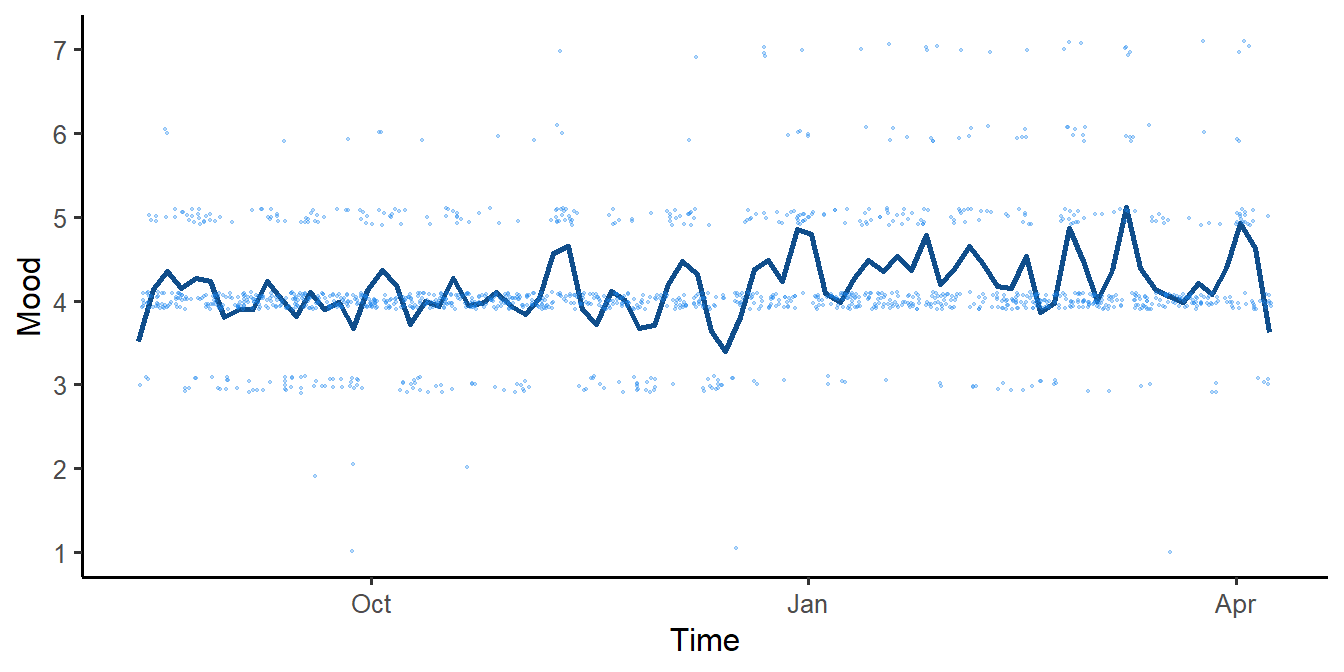
\includegraphics[width=1\linewidth]{mood_files/figure-latex/moodplot-1} 

}

\caption{34 weeks of mood data, from a single participant}\label{fig:moodplot}
\end{figure}

\subsection{Bipolar Unidimensional
Items}\label{bipolar-unidimensional-items}

\index{Mood assessment!Bipolar unidimensional}

Another option to assist respondents with the interpretation of one-item
mood ratings, is to use a bipolar scale. These items place two opposing
mood states at each end of the scale, for example by asking ``Please
rate your current mood on a scale of 0 to 100, on which 0 indicates
happy, and 100 indicates sad'' \citep{Vanrijsbergen2014}. This does
assume that the opposing mood states, such as happy and sad, are
mutually exclusive and thus cannot occur simultaneously. The
bipolar-unidimensional method was shown to be able to predict time to
relapse over 5.5 years in recurrently depressed out-patients, with 6.3\%
of variance in time to relapse explained. This percentage was comparable
to that of the HAM-D \citep{Rijsbergen2012}. Also, the scale was able to
detect relapse in patients with recurrent Major Depressive Disorder
(based on SCID-I interview) at a cut-off score of 55, and outperformed
the HAM-D and IDS-SR. However, 47\% of patients indicated by the VAS
scale did not fulfill formal criteria for relapse (false positives)
\citep{Vanrijsbergen2014}.

\section{Bag-of-Items}\label{bag-of-items}

\index{Mood assessment!Bag-of-Items}

In order to make sure all constructs of interest are measured, you can
also consider including a number of specific mood items in your EMA
questionnaire, rather than one general unipolar item or one bipolar
item. For example, you can ask respondents \emph{``How depressed are you
feeling right now?''} and \emph{``How anxious are you feeling right
now?''} \citep{Starr2012}. This strategy often leads to a `bag-of-items'
approach, where single items from various sources, such as existing
questionnaires, are combined into a new EMA questionnaire. A benefit of
this approach is that you can select items for which information on
validity and test-retest reliability is available. A downside is that
item scores can only be evaluated separately, rather that providing one
overall indication of mood or well-being.

Combining data from multiple items, such as mood and loneliness, in one
graph can provide respondents with insight in the interaction between
the constructs. In R two variables can easily be plotted together:

\begin{Shaded}
\begin{Highlighting}[]
\CommentTok{# Plotting multiple variables in one graph.}
\KeywordTok{library}\NormalTok{(ggplot2) }
\KeywordTok{library}\NormalTok{(emaph)}

\NormalTok{combined <-}\StringTok{ }\NormalTok{plotmood_down }\OperatorTok{+}\StringTok{ }
\StringTok{  }\KeywordTok{geom_point}\NormalTok{(}\DataTypeTok{data=}\NormalTok{csd, }\KeywordTok{aes}\NormalTok{(date,}\KeywordTok{as.numeric}\NormalTok{(mood_lonely)), }
    \DataTypeTok{size =}\NormalTok{ .}\DecValTok{3}\NormalTok{, }\DataTypeTok{alpha =}\NormalTok{ .}\DecValTok{3}\NormalTok{, }\DataTypeTok{position =} \KeywordTok{position_jitter}\NormalTok{(}\DataTypeTok{height =}\NormalTok{ .}\DecValTok{1}\NormalTok{),}
    \DataTypeTok{colour=}\StringTok{"indianred4"}\NormalTok{) }\OperatorTok{+}\StringTok{ }
\StringTok{  }\KeywordTok{geom_smooth}\NormalTok{(}\DataTypeTok{data=}\NormalTok{csd, }\KeywordTok{aes}\NormalTok{(date,}\KeywordTok{as.numeric}\NormalTok{(mood_lonely)), }
    \DataTypeTok{method =} \StringTok{"loess"}\NormalTok{, }\DataTypeTok{span =}\NormalTok{ .}\DecValTok{05}\NormalTok{, }\DataTypeTok{se =} \OtherTok{FALSE}\NormalTok{, }\DataTypeTok{colour=}\StringTok{"indianred2"}\NormalTok{)}
\KeywordTok{print}\NormalTok{(combined)}
\end{Highlighting}
\end{Shaded}

\begin{figure}

{\centering 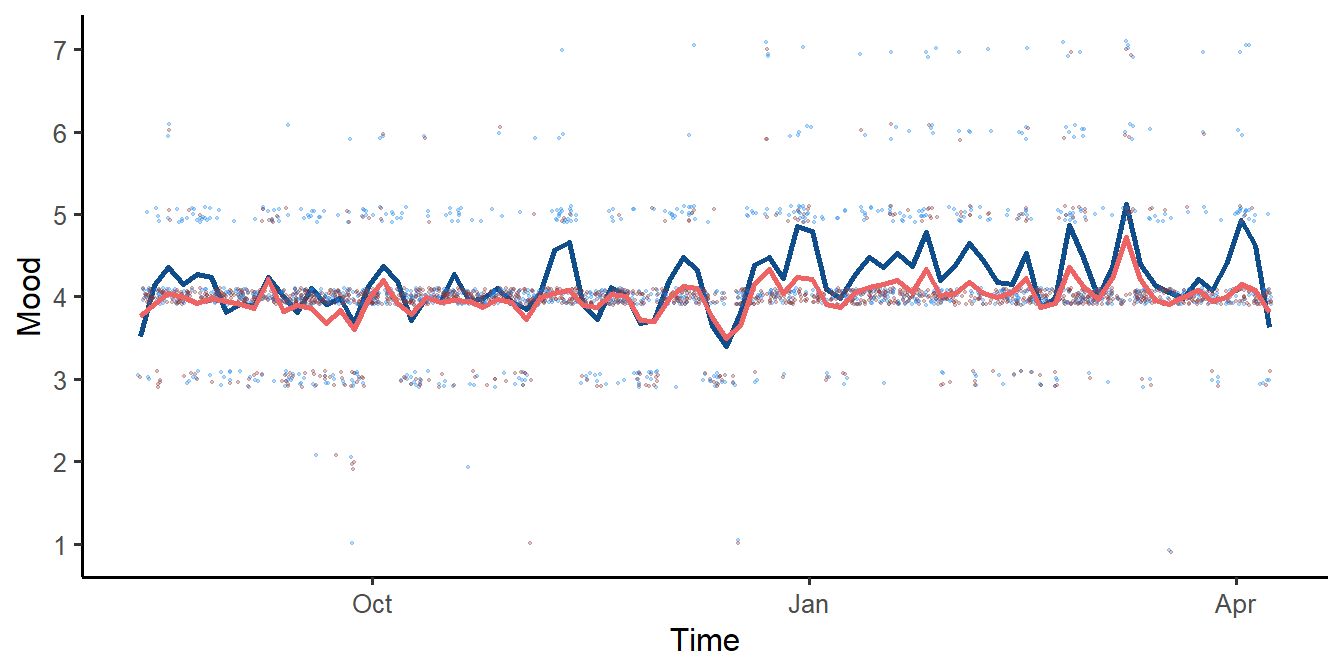
\includegraphics[width=1\linewidth]{mood_files/figure-latex/moodplotcombined-1} 

}

\caption{34 weeks of combined mood data, from a single participant}\label{fig:moodplotcombined}
\end{figure}

\section{Multi-dimensional Mood
Assessment}\label{multi-dimensional-mood-assessment}

\index{Mood assessment!Multi-dimensional}

Dimensional models assume that every affective state or emotion should
be described by the combined score on (at least) two items, instead of
just one. Over the past decades several multi-dimensional models have
been specified (for an overview, see \citet{sander2009}). In the context
of EMA, researchers most often base their items on the Circumplex model
\citep{russell1980circumplex} or the Negative/Positive affect (NA/PA)
theory \citep{watson1985}.

\subsection{The Circumplex Model}\label{the-circumplex-model}

\index{Mood assessment!Circumplex model}
\index{Mood assessment!Pick-a-mood scale}

The Circumplex Model of affect \citep{russell1980circumplex, Posner2005}
argues that all mood states are a linear combination of two independent,
bipolar scales: valence (ranging from unpleasant to pleasant) and
arousal/activation (ranging from low to high arousal). Combining scores
on these scales places the affective states in a circle on one of four
quadrants (see Figure \ref{fig:circumplexrussel}). States within one
quadrant are believed to be positively correlated, while states in the
opposing quadrant are thought to be negatively correlated.

\begin{figure}

{\centering 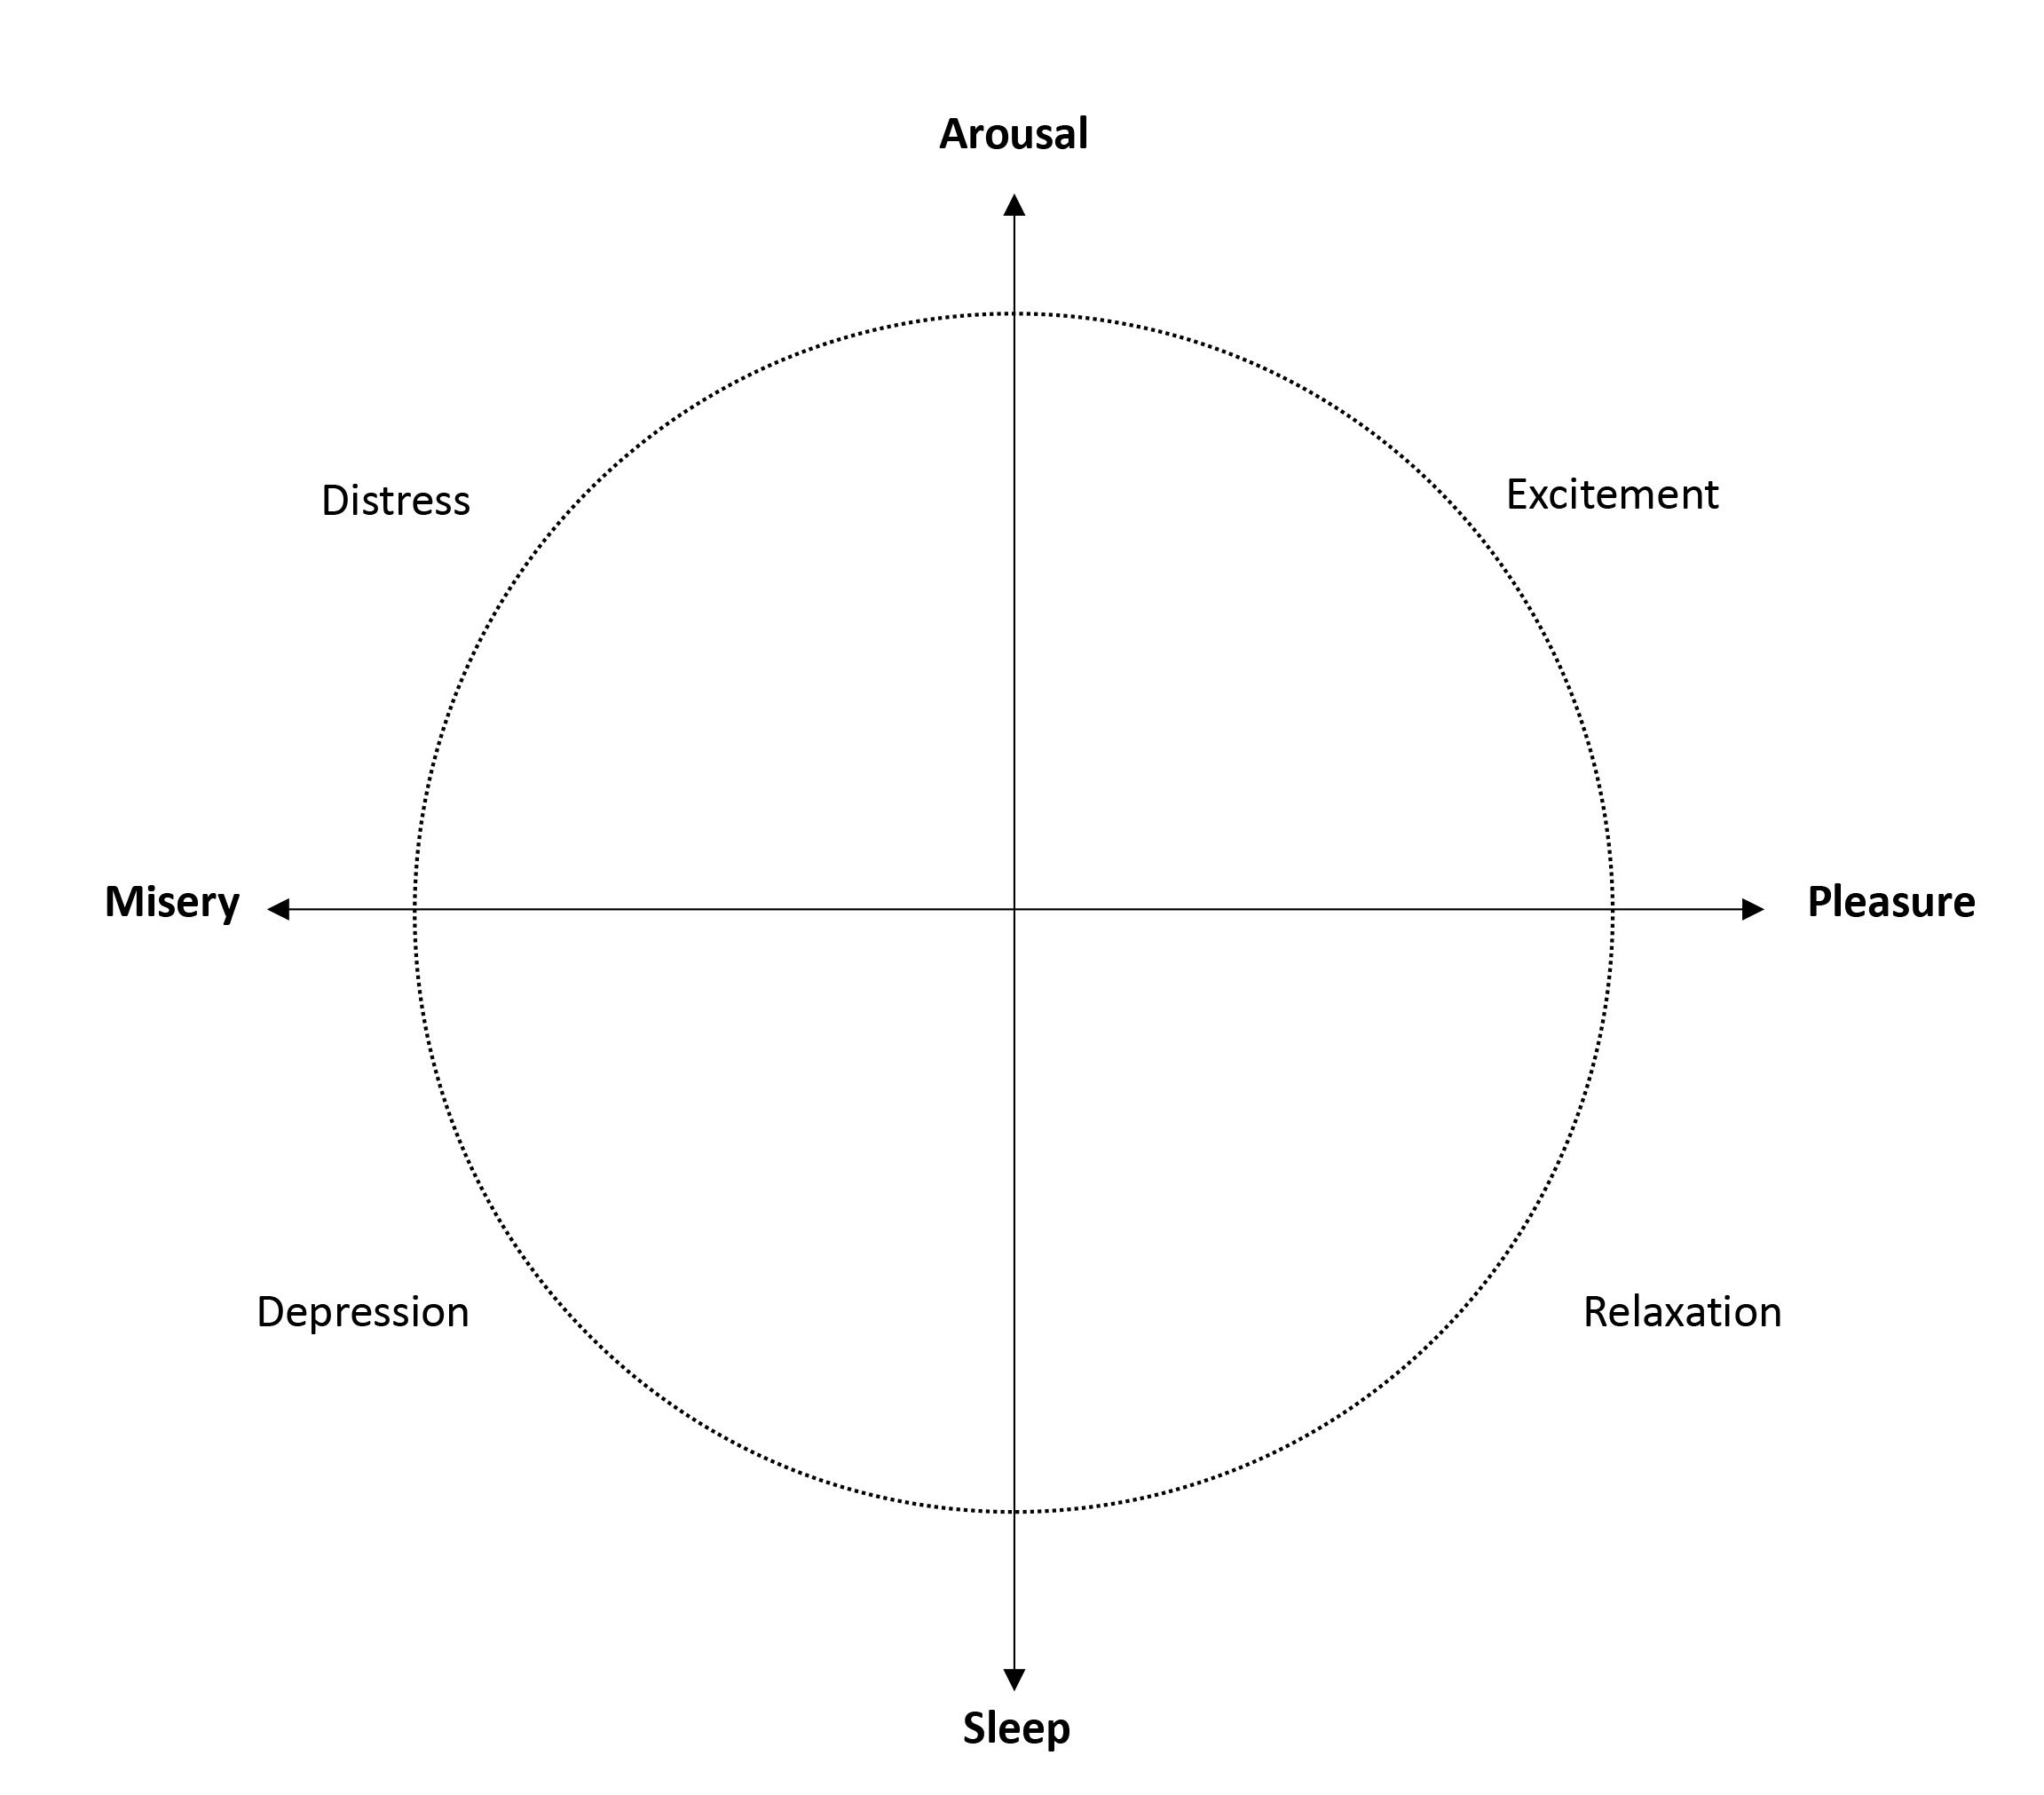
\includegraphics[width=0.6\linewidth]{images/outcomes/Russell1980} 

}

\caption{Russell's Circumplex model of affect.}\label{fig:circumplexrussel}
\end{figure}

There are several options to operationalize the Circumplex model in EMA
research. For example, respondents can rate valence and arousal on two
VAS scales. The most pragmatic approach is to report both scale scores
separately \citep{Asselbergs2016}. Alternatively, scores can be combined
to give insight into which of the four mood states (quadrants)
respondents fall:

\begin{itemize}
\tightlist
\item
  Low aroused - unpleasant
\item
  Low aroused - pleasant
\item
  High aroused - unpleasant
\item
  High aroused - pleasant
\end{itemize}

A downside of the Circumplex model is that the concepts of valence and
arousal can be hard to convey to respondents, especially when translated
to other languages, such as Dutch. One alternative is to adjust the
scale ends, for example using ``extreme sleepiness'' and ``extreme high
energy'' \citep{sharar2016}. Another option is to use pictures or
emoticons, rather than language. For this purpose, DeSmet and colleagues
developed the pick-a-mood scale, which is a pictorial self-report scale
\citep{Desmet2016}. The scale builds on the circumplex model and adds
the third dimension ``dominance'' (level of experienced control over the
mood state), rendering eight (instead of four) different mood states and
one neutral state (see Figure \ref{fig:pickamood}).

\begin{figure}

{\centering 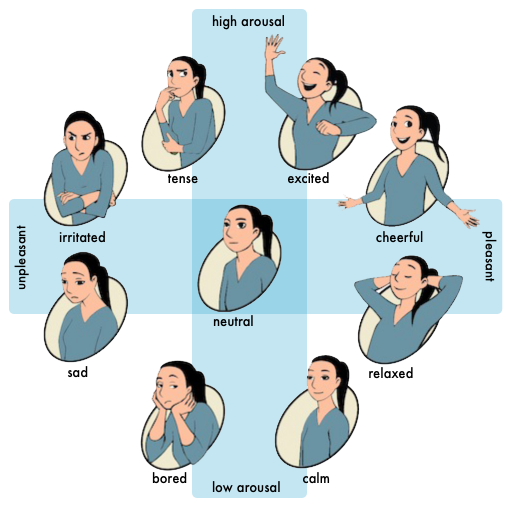
\includegraphics[width=0.5\linewidth]{images/outcomes/Circumplex-Pick-A-Mood} 

}

\caption{The Pick-A-Mood Circle.}\label{fig:pickamood}
\end{figure}

\subsection{Negative \& Positive Affect}\label{negative-positive-affect}

\index{Positive and Negative Affect} \index{Mood assessment!PA/NA}
\index{Positive Affect|see{Mood assessment!PA/NA}}
\index{Positive and Negative Affect!PANAS|see{Mood assessment}}

Watson and Tellegen \citep{watson1985} also specified the underlying
theory of the Circumplex model, arguing that the diagonal quadrants
represent Positive and Negative affect (PA/NA) and that these two terms
are the main dimensions of affect \citep{Watson1999}. PA ranges from
sadness to high energy, NA from calmness to distress \citep{Watson1988}.
While bipolar-unidimensional assessment assumes that positive and
negative affect are mutually exclusive, the PA/NA affect model assumes
that these mood states can occur simultaneously. Watson and Clark
\citep{Watson1997} for example, showed a moderate correlation between
the two constructs (r = .32). In order to measure Positive and Negative
Affect, a designated Positive and Negative Affect Schedule was developed
by Watson, Clark and Tellegen \citep{Watson1988}. Respondents are asked
to indicate \emph{``to what extent you feel this way right now''} on 20
affect items. The scale uses a 5-point Likert-scale, ranging from 1
(very slightly or not at all) to 5 (very) \citep{Watson1999}. Items
include:

\begin{itemize}
\tightlist
\item
  Negative Affect (10): afraid, scared, nervous, jittery, irritable,
  hostile, guilty, ashamed, upset, distressed
\item
  Positive Affect (10): active, alert, attentive, determined,
  enthusiastic, excited, inspired, interested, proud, strong
\end{itemize}

There are several short-forms available. For example, Wichers and
colleagues created a 10-item short-form of the PANAS for their EMA
studies. The items were based on the PANAS and their own experience with
EMA \citep{Wichers2012}. Using factor analyses, the following 7-point
Likert items were chosen for the questionnaire:

\begin{itemize}
\tightlist
\item
  Negative affect (6): insecure, lonely, anxious, low, guilty,
  suspicious.
\item
  Positive affect (4): cheerful, content, energetic, enthusiastic.
\end{itemize}

PA and NA were calculated as the average score across all items and
weighted for their factor loadings \citep{Wichers2012}. In r, such a
factor analysis can be executed as follows:

\begin{Shaded}
\begin{Highlighting}[]
\CommentTok{# Performing a factor analysis.}
\KeywordTok{library}\NormalTok{(dplyr)}
\KeywordTok{library}\NormalTok{(tibble)}

\NormalTok{items2 <-}\StringTok{ }\NormalTok{csd }\OperatorTok
\StringTok{  }\KeywordTok{select}\NormalTok{(}\KeywordTok{c}\NormalTok{(}
   \StringTok{"mood_relaxed"}\NormalTok{, }\StringTok{"mood_satisfi"}\NormalTok{,}
   \StringTok{"mood_enthus"}\NormalTok{, }\StringTok{"mood_cheerf"}\NormalTok{,}
   \StringTok{"mood_strong"}\NormalTok{, }\StringTok{"mood_down"}\NormalTok{,}
   \StringTok{"mood_lonely"}\NormalTok{, }\StringTok{"mood_anxious"}\NormalTok{, }
   \StringTok{"mood_guilty"}\NormalTok{ )) }\OperatorTok
\StringTok{  }\KeywordTok{scale}\NormalTok{(.) }\OperatorTok
\StringTok{  }\KeywordTok{as.tibble}\NormalTok{(.) }\OperatorTok
\StringTok{  }\KeywordTok{mutate_all}\NormalTok{(}\KeywordTok{funs}\NormalTok{(}\KeywordTok{residuals}\NormalTok{(stats}\OperatorTok{::}\KeywordTok{arima}\NormalTok{(., }\DataTypeTok{order =} \KeywordTok{c}\NormalTok{(}\DecValTok{1}\NormalTok{,}\DecValTok{0}\NormalTok{,}\DecValTok{0}\NormalTok{)))))}

\KeywordTok{require}\NormalTok{(psych)}

\NormalTok{correlations <-}\StringTok{ }\KeywordTok{cor}\NormalTok{(items2, }\DataTypeTok{use =} \StringTok{"complete.obs"}\NormalTok{)}
\NormalTok{model <-}\StringTok{ }\KeywordTok{fa}\NormalTok{(items2,}
               \DataTypeTok{nfactors =} \DecValTok{2}\NormalTok{,}
               \DataTypeTok{rotate =} \StringTok{"oblimin"}\NormalTok{,}
               \DataTypeTok{fm =} \StringTok{"pa"}\NormalTok{,}
               \DataTypeTok{scores =} \StringTok{"regression"}\NormalTok{)}

\KeywordTok{colnames}\NormalTok{(model}\OperatorTok{$}\NormalTok{loadings) <-}\StringTok{ }\KeywordTok{c}\NormalTok{(}\StringTok{"PA"}\NormalTok{, }\StringTok{"NA"}\NormalTok{)}
\NormalTok{psych}\OperatorTok{::}\KeywordTok{fa.diagram}\NormalTok{(model)}
\end{Highlighting}
\end{Shaded}

\begin{figure}

{\centering 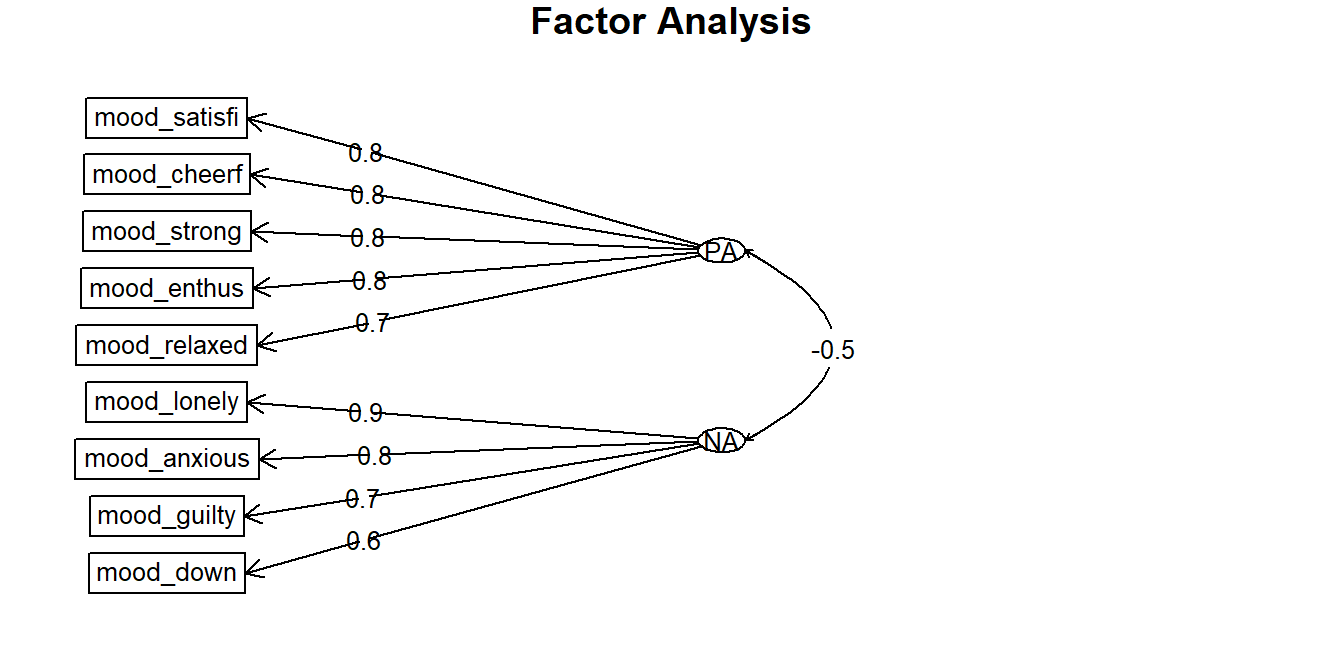
\includegraphics[width=1\linewidth]{mood_files/figure-latex/moodfa-1} 

}

\caption{Factor analysis of scores of 9 EMA items, revealing two factors:  Positive Affect (PA) and Negative Affect (NA).}\label{fig:moodfa}
\end{figure}

\chapter{Activity}\label{activity}

\index{EMA!Passive EMA} \index{Actigraphy} \index{Geotracking}

The objective study of human physical activity is one of the exciting
opportunities created by passive EMA \citep{Marszalek2014}. Through
technological advances in mobile sensing, we are now able to
continuously monitor (in-)activity of participants in every-day life,
with little to no participant burden.

While questions remain with regard to the validity, reliability and
clinical utility of passive EMA of specific activities, such as
(disturbed) sleep, sedentary behavior, and energy expenditure
\citep[see, e.g.,][]{Feehan2018, Gomersall2016}, an increasing number of
mental health studies are including activity tracking devices to better
understand sleep habits, circadian rhythm disorders and depression
\citep[see, e.g.,][]{Saeb2015, Saunders2016, Tahmasian2013}.

In this chapter, we will discuss two passive EMA methods to assess
physical activity: actigraphy and geotracking. Of these two, actigraphy
has been used most in human clinical research. However, due to the
massive adoption of smartphones, researchers increasingly collect
geolocation data as well, inspired perhaps by the elaborate geolocation
data analysis techniques that have been developed in the past decades in
wildlife telemetry research \citep{tomkiewicz2010global}.

\begin{figure}

{\centering 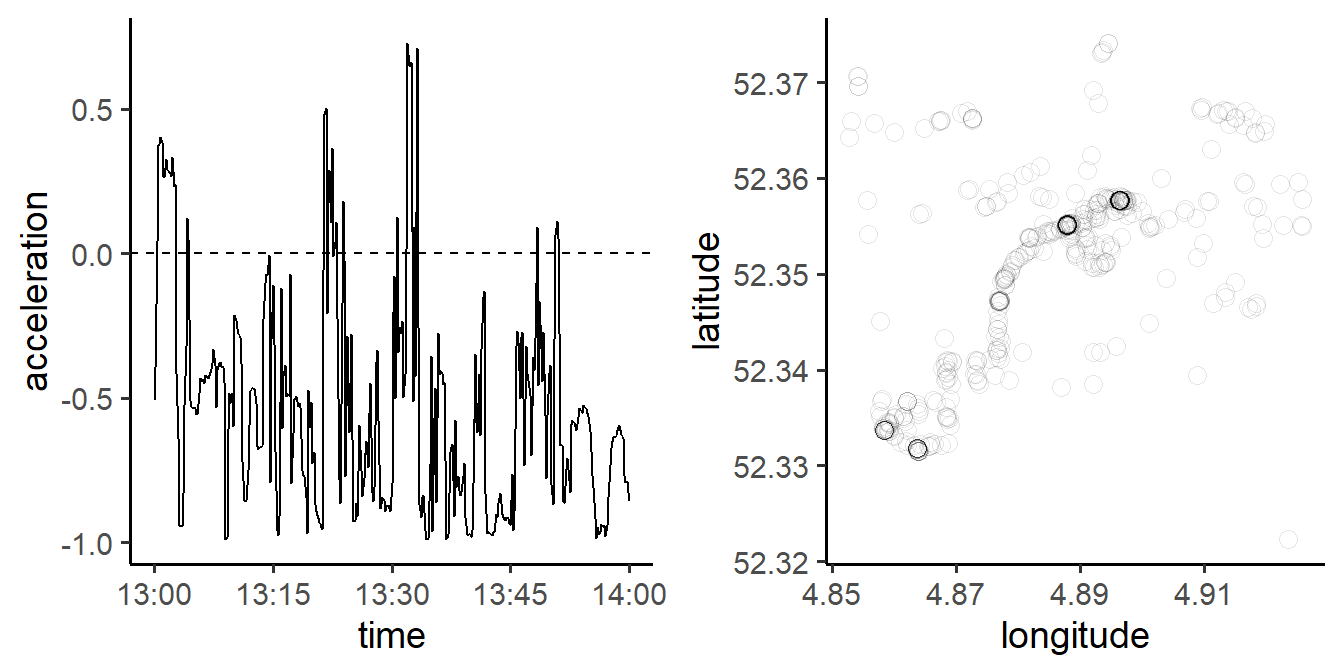
\includegraphics[width=0.95\linewidth]{activity_files/figure-latex/accgps-1} 

}

\caption{Actigraphy (left) and Geotracking (right): two methods for passive ecological momentary assessment of activity.}\label{fig:accgps}
\end{figure}

\section{Actigraphy}\label{actigraphy}

\index{Actigraphy} \index{Accelerometer} \index{GENEActive}

Accelerometers are micro electro-mechanical systems (MEMS) that measure
changes in acceleration forces (i.e., both static forces - earth's
gravity - and dynamic forces - caused by movement), typically
simultaneously on the vertical (Y), horizontal right-left (X) and
horizontal front-back axis (Z). Through actigraphy, we study the
frequency, duration, and intensity of physical activity. Figure
\ref{fig:genea-one-hour} shows one hour of data collected from a
wrist-worn GENEActiv accelerometer. As can be seen, three accelerometers
(X, Y, Z) were simultaneously providing data. Data were sampled with a
frequency of 30 Hertz (Hz; thirty measurements per second - which is
common), but sub-sampled here to 0.1Hz (one measurement every 10
seconds), for practical reasons. If we would have plotted the data at
30Hz, the plot would have included 108.000 data points. At 0.1Hz, this
reduces to 360 points.

\begin{figure}

{\centering 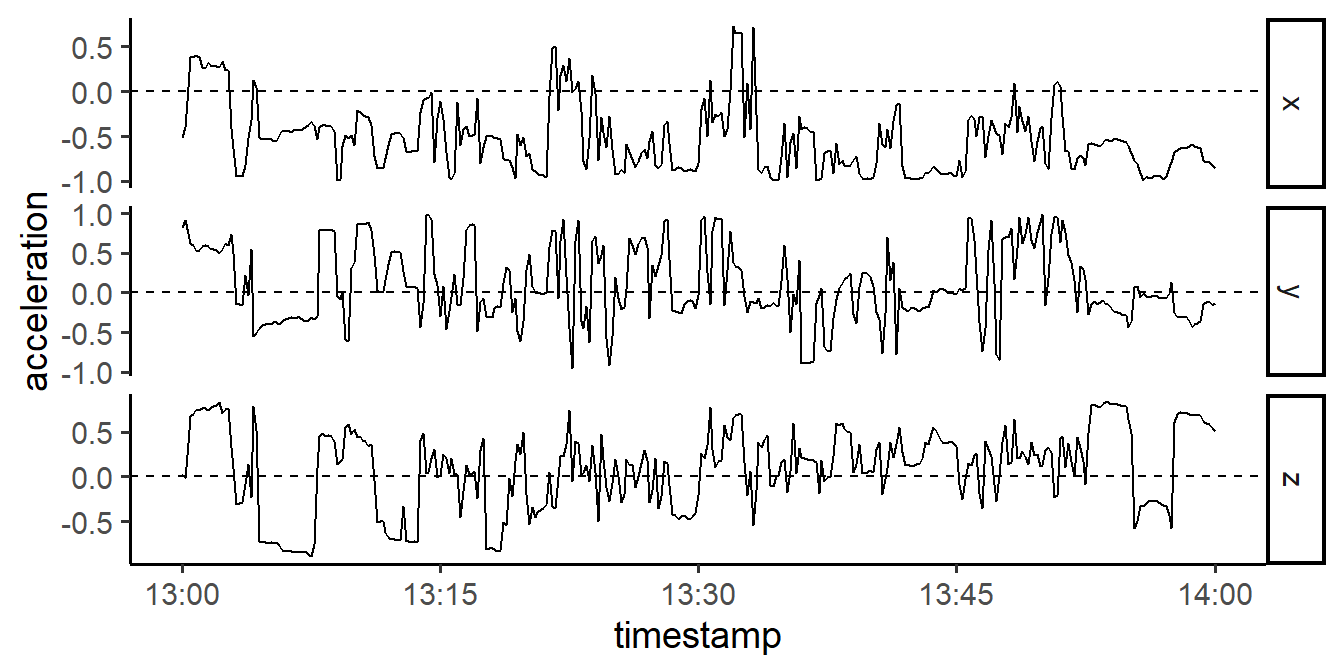
\includegraphics[width=1\linewidth]{activity_files/figure-latex/genea-one-hour-1} 

}

\caption{One hour of raw data collected with a wrist-worn GENEActiv accelerometer, sub-sampled to 10-second epochs (0.1 Hz)}\label{fig:genea-one-hour}
\end{figure}

Data shown are included in package \texttt{emaph}, and the R-code to
reproduce the plot is listed below. Use this to familiarize yourself
with actigraphy data. If you want to see how sub-sampling affects the
number of points to plot, for example, you can set different values in
the \texttt{round\_date} function. For example, to get a point for each
five seconds (0.2Hz), you would set the argument of this function to
\texttt{5\ seconds}.

\begin{Shaded}
\begin{Highlighting}[]
\CommentTok{# Plot one hour of emaph accelerometer data (of person 1).}
\KeywordTok{library}\NormalTok{(dplyr)}
\KeywordTok{library}\NormalTok{(ggplot2)}
\NormalTok{d <-}\StringTok{  }\KeywordTok{subset}\NormalTok{(emaph}\OperatorTok{::}\NormalTok{genea, timestamp }\OperatorTok{>}\StringTok{ "2018-06-01 13:00"} \OperatorTok{&}
\StringTok{                           }\NormalTok{timestamp }\OperatorTok{<}\StringTok{ "2018-06-01 14:00"} \OperatorTok{&}
\StringTok{                           }\NormalTok{id }\OperatorTok{==}\StringTok{ }\DecValTok{1}\NormalTok{)}
\NormalTok{d}\OperatorTok{$}\NormalTok{timestamp <-}\StringTok{ }\NormalTok{lubridate}\OperatorTok{::}\KeywordTok{round_date}\NormalTok{(d}\OperatorTok{$}\NormalTok{timestamp, }\StringTok{"10 seconds"}\NormalTok{)}
\NormalTok{d <-}\StringTok{ }\NormalTok{d }\OperatorTok\StringTok{ }\KeywordTok{group_by}\NormalTok{(timestamp) }\OperatorTok\StringTok{ }\KeywordTok{summarise_all}\NormalTok{(}\DataTypeTok{.funs =}\NormalTok{ mean) }\OperatorTok\StringTok{ }
\StringTok{  }\NormalTok{tidyr}\OperatorTok{::}\KeywordTok{gather}\NormalTok{(}\DataTypeTok{key =} \StringTok{"sensor"}\NormalTok{, }\DataTypeTok{value =} \StringTok{"value"}\NormalTok{, x, y, z)}

\KeywordTok{ggplot}\NormalTok{(d, }\KeywordTok{aes}\NormalTok{(timestamp, value)) }\OperatorTok{+}\StringTok{ }\KeywordTok{geom_line}\NormalTok{() }\OperatorTok{+}\StringTok{ }
\StringTok{  }\KeywordTok{geom_hline}\NormalTok{(}\DataTypeTok{yintercept =} \DecValTok{0}\NormalTok{, }\DataTypeTok{linetype =} \DecValTok{2}\NormalTok{) }\OperatorTok{+}\StringTok{ }\KeywordTok{facet_grid}\NormalTok{(}\DataTypeTok{rows =} \KeywordTok{vars}\NormalTok{(sensor) , }\DataTypeTok{scales =} \StringTok{"free_y"}\NormalTok{)}
\end{Highlighting}
\end{Shaded}

\subsection{Data cleaning}\label{data-cleaning}

\index{Datamanagement!Data cleaning} \index{GGIR} \index{GENEARead}

Raw accelerometer data need to be cleaned before analyses can be run.
Typical data import work-flows include re-calibration (to reduce
systematic measurement error), the detection of non-wear periods (to
ensure that non-informative data are removed), sub-sampling (reducing
the sample rate to reduce analysis time) and filtering/aggregation (to
smoothen the signal and reduce the impact of outliers, measurement error
and occasional missing values). Study results can be highly dependent on
these initial steps, which, unfortunately, are also complex and
time-consuming. Specialized R-packages exist to help you with this (see,
for example, package \texttt{GGIR} and \texttt{GENEARead}, which are
described in more detail in Chapter \ref{rcat}).

\subsection{Feature Extraction}\label{feature-extraction}

\index{ENMO} \index{SVM}

Properties of the signals that are of interest are highly dependent on
the focus of the study. Highly detailed analysis of local peaks in the
signal might be needed, for instance to reveal an association between
activity and reported events. But analyses can also be more global, for
instance when accelerometer data are used to study circadian rhythms in
activity. Several approaches exist to combine the X, Y, Z measurements
into a single meaningful metric. Two popular metrics are the `Signal
Vector Magnitude' (SVM) and the `Euclidean Norm Minus One' (ENMO).
Validation studies suggest that ENMO should be the preferred metric
\citep{VanHeest2014, VanHeest2015}, although recent findings also
suggest that alternative metrics should perhaps be considered when
sedentary and light activities are of interest \citep{Bai2016}.

SVM and ENMO are closely related. SVM is the magnitude of the raw
tri-axial signals (the Euclidean distance in the three-dimensional
space), i.e. \emph{SVM = sqrt(x\^{}2 + y\^{}2 + z\^{}2)}. ENMO is the
corrected SVM: the vector magnitude remaining after removing one Earth
Standard Gravitational unit (1g = 9.81 m/s\^{}2), i.e. \emph{ENMO = SVM
- 1}. The metrics can, in principle, be calculated for each \{x, y,
z\}-data point in the raw series. Typically, however, the metrics are
calculated for time-windows (called \emph{epochs}), in which case the
mean can be used to characterize the overall activity in each epoch.

Figure \ref{fig:genea-one-day} shows the development of ENMO over one
day, as sampled by GENEActiv accelerometers that were worn by a young
adult (top) and a middle-aged person (bottom). This figure is much
easier to interpret than the plot of the raw x-y-z values in Figure
\ref{fig:genea-one-hour}. Activity levels over the day follow a similar
pattern, but the activity levels in the two plots are strikingly
different. Age appears to matter here: activity levels of the
middle-aged person are consistently lower than those of the young adult.

\begin{figure}

{\centering 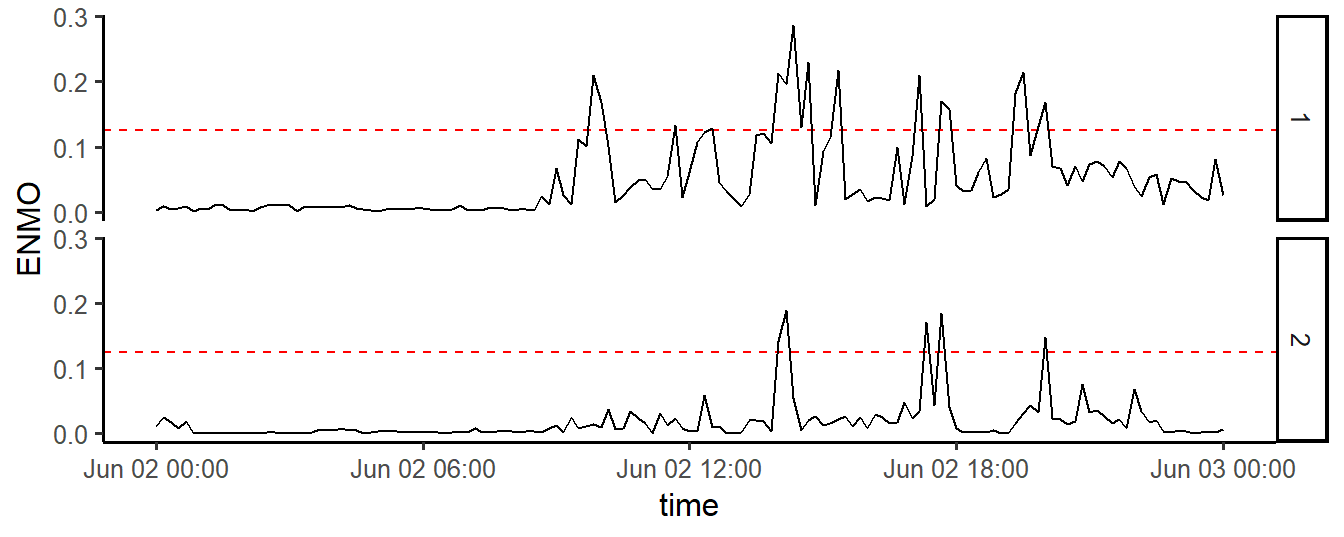
\includegraphics[width=1\linewidth]{activity_files/figure-latex/genea-one-day-1} 

}

\caption{One day of data of the two persons in the GENEA data set of package 'emaph', summarised with ENMO, in 10-minute epochs}\label{fig:genea-one-day}
\end{figure}

\index{MVPA}

For SVM and ENMO, cut-off values for various activity classes have been
determined \citep{Dasilva2014, Hildebrand2014, Kim2017, Rowlands2016}.
Although these cut-offs vary somewhat from study to study, a common ENMO
cut-off for Moderate-to-Vigorous-Physical-Activity (MVPA) is 0.125g (125
milligravity units; Femke Lamers, personal communication, 15 november
2018). The dotted line in Figure \ref{fig:genea-one-day} marks this
cut-off.

With this cut-off, we can summarize the two series shown in Figure
\ref{fig:genea-one-day} by the number of times on which ENMO is higher
than the MVPA cut-off. The daily MVPA-count for the young adult is 17.
For the middle-aged person, this is 5: considerably lower.

You should be aware that the choice of the width of the epoch matters
when MVPA-counts are calculated. By averaging values in each window,
ENMO acts as a smoother, which may prevent you from the detection of
short bursts of activity when the window is large. If we would have used
a 5-second window to generate Figure \ref{fig:genea-one-day}, for
example, the MVPA-counts would go up considerably for each person.

\section{Geotracking}\label{geotracking}

\index{Geotracking}

\subsection{The Geographic Coordinate
System}\label{the-geographic-coordinate-system}

\index{Geographic Coordinate system} \index{Longitude} \index{Latitude}

In the geographic coordinate system, each location on the earth is
uniquely represented by two numbers: \emph{Latitude} and
\emph{Longitude}. Latitude marks the north--south position of a point on
the earth's surface, and longitude marks the east-west position (see
Figure \ref{fig:longlat}). The center of Amsterdam, for example, is
\{latitude: 52.37022; longitude: 4.89517\}, which can be verified by
punching these numbers in \href{https://tinyurl.com/ybxxk99a}{Google
maps}.

\begin{figure}[!h]

{\centering 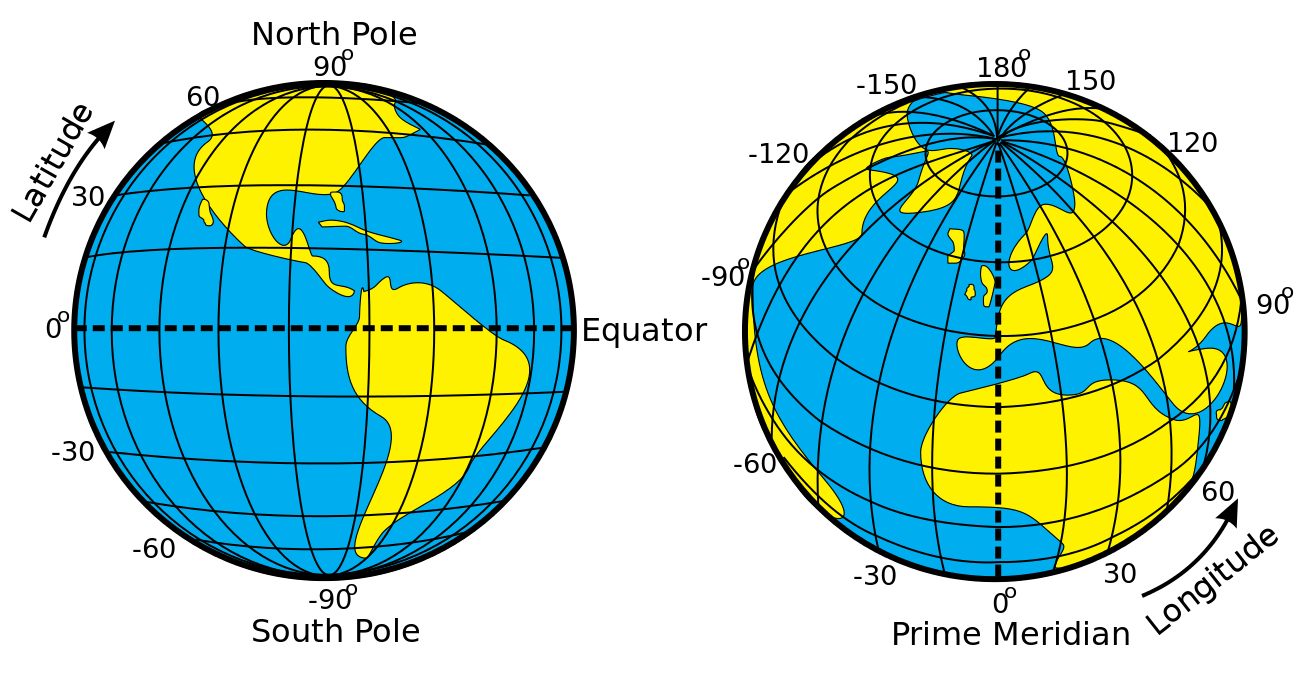
\includegraphics[width=0.75\linewidth]{images/activity/Latitude_and_Longitude_of_the_Earth} 

}

\caption{Latitude and Longtitude of the Earth (source: WikiPedia).}\label{fig:longlat}
\end{figure}

\subsection{The Global Positioning
System}\label{the-global-positioning-system}

\index{GPS}

The Global Positioning System (GPS) is a satellite-based
radio-navigation system that provides geolocation and time information.
With GPS-receivers, latitude and longitude can be determined, to track
geographical locations and movement. Due to the increasing ease with
which GPS-data can be collected via modern smartphones, recent years
have witnessed a marked increase in the use of GPS-based activity
measures in the study of mental health.

Figure \ref{fig:fourweekgps} shows GPS-data of two people, collected
over a period of four weeks, via the Google timeline smartphone app.
Data can be found in the \texttt{emaph} package (see
\texttt{?locations}).

\begin{Shaded}
\begin{Highlighting}[]
\CommentTok{# Plot four-week location history of emaph location data}
\KeywordTok{library}\NormalTok{(ggplot2)}
\KeywordTok{library}\NormalTok{(emaph)}

\NormalTok{d <-}\StringTok{ }\KeywordTok{subset}\NormalTok{(locations,}
\NormalTok{            accuracy }\OperatorTok{<=}\StringTok{ }\DecValTok{50} \OperatorTok{&}
\StringTok{              }\NormalTok{lon }\OperatorTok{>=}\StringTok{  }\FloatTok{4.80} \OperatorTok{&}\StringTok{ }\NormalTok{lon }\OperatorTok{<=}\StringTok{  }\FloatTok{5.00} \OperatorTok{&}
\StringTok{              }\NormalTok{lat }\OperatorTok{>=}\StringTok{ }\FloatTok{52.25} \OperatorTok{&}\StringTok{ }\NormalTok{lat }\OperatorTok{<=}\StringTok{ }\FloatTok{52.50}\NormalTok{) }\OperatorTok\StringTok{ }
\StringTok{  }\KeywordTok{sample_n}\NormalTok{(}\DecValTok{4000}\NormalTok{)}
  
\KeywordTok{ggplot}\NormalTok{(d, }\KeywordTok{aes}\NormalTok{(lon, lat)) }\OperatorTok{+}
\StringTok{  }\KeywordTok{geom_point}\NormalTok{(}\DataTypeTok{alpha =}\NormalTok{ .}\DecValTok{2}\NormalTok{,  }\DataTypeTok{shape =} \DecValTok{21}\NormalTok{, }\DataTypeTok{size =} \DecValTok{3}\NormalTok{) }\OperatorTok{+}
\StringTok{  }\KeywordTok{xlab}\NormalTok{(}\StringTok{"longitude"}\NormalTok{) }\OperatorTok{+}\StringTok{ }\KeywordTok{ylab}\NormalTok{(}\StringTok{"latitude"}\NormalTok{) }\OperatorTok{+}\StringTok{ }
\StringTok{  }\KeywordTok{facet_wrap}\NormalTok{(}\OperatorTok{~}\StringTok{ }\NormalTok{id)}
\end{Highlighting}
\end{Shaded}

\begin{figure}

{\centering 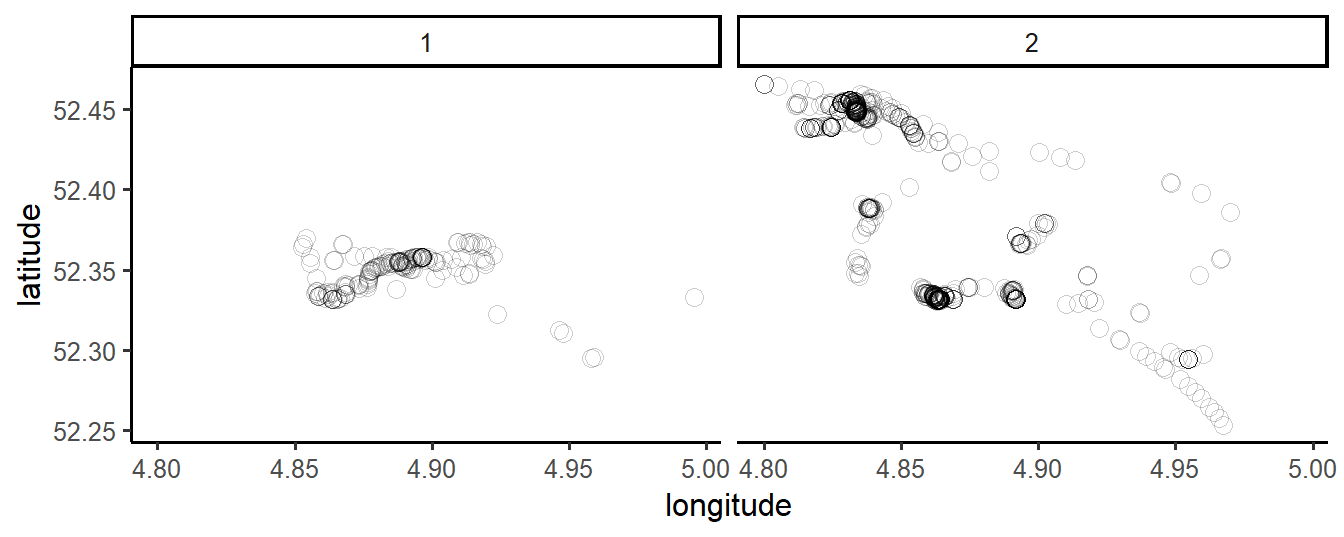
\includegraphics[width=1\linewidth]{activity_files/figure-latex/fourweekgps-1} 

}

\caption{Four-week location history of two people, collected with Google Timeline.}\label{fig:fourweekgps}
\end{figure}

Data-points are superposed, using transparent colors, to make a
distinction between locations that were visited once (light areas) and
places that were visited many times (darker areas). From the plot, we
learn that these two people both lived and worked in the Amsterdam area
(latitude and longitude are close to the coordinates of Amsterdam
center). We also see that they shared a frequently visited location
(they were co-workers, working in the same building). Locations of
person 1 reveal that this person's home was probably in Amsterdam, while
the locations of person 2 show that this person's home was probably
located in an Amsterdam suburb. Commuting patterns (i.e., the recurrent
traveling between the place of residence and place of work) are clearly
visible.

It should be noted, though, that person 1 contributed much less data (n
= 722) than person 2 (n = 14031). This can be explained by the different
devices that were used by both: Person 1 used an iPhone (with standard
GPS-settings) and Person 2 used a Sony Z1 Android (with high-precision
GPS features enabled). This device-related variability in GPS sample
rates and accuracy is one of the primary challenges of naturalistic EMA
research and EMI applications.

The problem with the (in)accuracy of GPS-data is further illustrated by
Figure \ref{fig:nightcrawl}, in which all data points are plotted that
were registered by the smartphone of person 2 between 02:00 and 06:00,
At those hours, the person was sleeping, in the bedroom of his house. He
did not move. Yet, if we would take the GPS-data for granted, he
regularly took a nightly random walk in the park. The red dot in the
figure marks the median coordinate. This coordinate is very accurate: it
marks the bedroom. All individual data points, however, fail to identify
this location.

\begin{figure}

{\centering 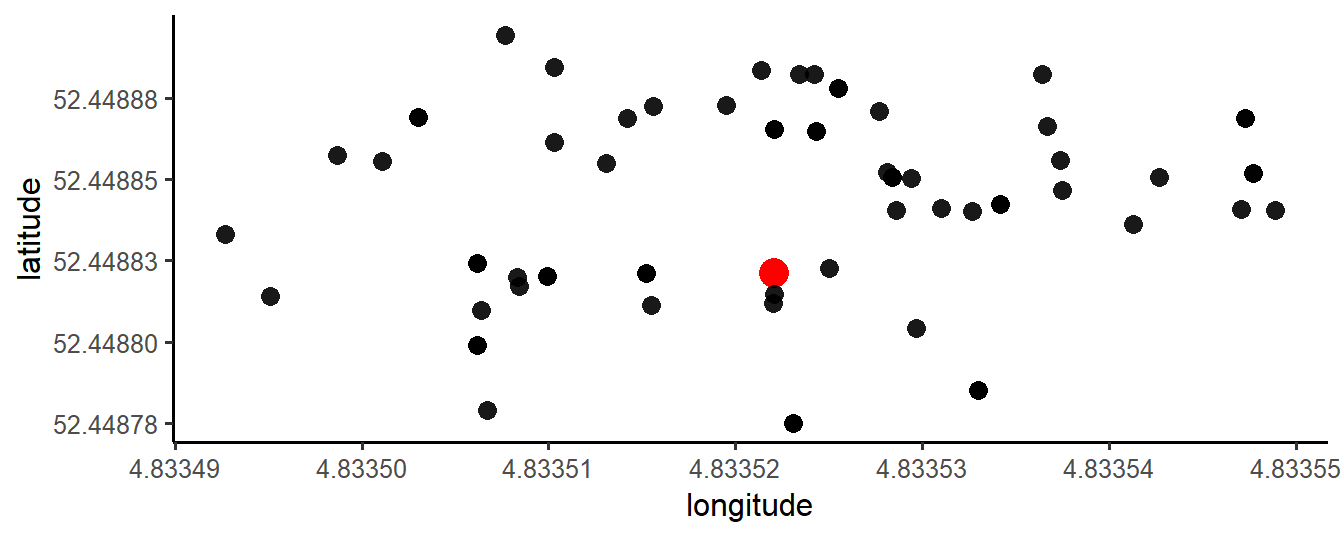
\includegraphics[width=1\linewidth]{activity_files/figure-latex/nightcrawl-1} 

}

\caption{Nightly GPS-fluctuations, revealing inaccurate location measurements}\label{fig:nightcrawl}
\end{figure}

\subsection{GPS-based Activity
Measures}\label{gps-based-activity-measures}

Raw GPS-data reflect series of locations rather than activity per se.
However, measures of activity can be extracted from these data.

Table \ref{tab:GPSfeatures} shows some of the measures that were derived
from GPS data in a small (n = 28) study exploring the correlation
between passive EMA data and depression, conducted by researchers of
Northwestern University \citep{Saeb2015}. The researchers calculated
total distance, location variance, the number of places visited by the
participants during the study, the percentage of time spent at home
(defined as a top 3 place which was most frequently visited between
24:00 and 6:00), and circadian movement - the consistency of location
visits based on a 24-hour period. Circadian movement and location
variance were found to be correlated with PHQ-9 scores in this study,
but not - however - in a follow-up study, which included more
participants \citep{Saeb2017}.

\begin{longtable}[]{@{}ll@{}}
\caption{\label{tab:GPSfeatures} Activity measures that can be derived from
a GPS data set.}\tabularnewline
\toprule
\begin{minipage}[b]{0.34\columnwidth}\raggedright\strut
\textbf{Name}\strut
\end{minipage} & \begin{minipage}[b]{0.60\columnwidth}\raggedright\strut
\textbf{Formula}\strut
\end{minipage}\tabularnewline
\midrule
\endfirsthead
\toprule
\begin{minipage}[b]{0.34\columnwidth}\raggedright\strut
\textbf{Name}\strut
\end{minipage} & \begin{minipage}[b]{0.60\columnwidth}\raggedright\strut
\textbf{Formula}\strut
\end{minipage}\tabularnewline
\midrule
\endhead
\begin{minipage}[t]{0.34\columnwidth}\raggedright\strut
Total distance between locations\strut
\end{minipage} & \begin{minipage}[t]{0.60\columnwidth}\raggedright\strut
\(\sum(distance((lat_{t}, lon_{t}), (lat_{t-1}, lon_{t-1})\)\strut
\end{minipage}\tabularnewline
\begin{minipage}[t]{0.34\columnwidth}\raggedright\strut
Location variance\strut
\end{minipage} & \begin{minipage}[t]{0.60\columnwidth}\raggedright\strut
\(log(\sigma_{lon}^2 + \sigma_{lat}^2)\)\strut
\end{minipage}\tabularnewline
\begin{minipage}[t]{0.34\columnwidth}\raggedright\strut
N Places\strut
\end{minipage} & \begin{minipage}[t]{0.60\columnwidth}\raggedright\strut
k-means(loc, lat)\strut
\end{minipage}\tabularnewline
\begin{minipage}[t]{0.34\columnwidth}\raggedright\strut
Home Stay\strut
\end{minipage} & \begin{minipage}[t]{0.60\columnwidth}\raggedright\strut
time(cluster{[}home{]}) / time(clusters{[}j{]})\strut
\end{minipage}\tabularnewline
\begin{minipage}[t]{0.34\columnwidth}\raggedright\strut
Circadian Movement\strut
\end{minipage} & \begin{minipage}[t]{0.60\columnwidth}\raggedright\strut
\(\sum(psd(f_i) / (i1 - i2)\)\strut
\end{minipage}\tabularnewline
\bottomrule
\end{longtable}

\part{Analytic Approaches}\label{part-analytic-approaches}

\chapter{Feature Extraction}\label{features}

EMA data are streams: time-series that represent processes which may
span hours, days, weeks or even months. To the beginning EMA researcher,
it may not be immediately clear how to deal with these data. How, for
example, can these series be summarized to study differences between
individuals or changes within individuals over time? What `qualities' or
`features' of a time-series should be considered? What are the available
options? In this chapter, we will discuss some of the features that can
be extracted from EMA time-series.

\section{Simulated EMA Time-series
Example}\label{simulated-ema-time-series-example}

\index{Simulating data}

We will focus on a simulated three-week time-series of EMA mood
responses of a single person, in which ratings were collected five times
per day (using the \texttt{generate\_features\_dataset} function of
package \texttt{emaph}). Figure \ref{fig:feat-plot} shows a plot of the
simulated scores.

Stare at the figure for a moment. How would you characterize the
development of scores over time? What features would you want to
extract? How would you quantify these features?

\begin{figure}

{\centering 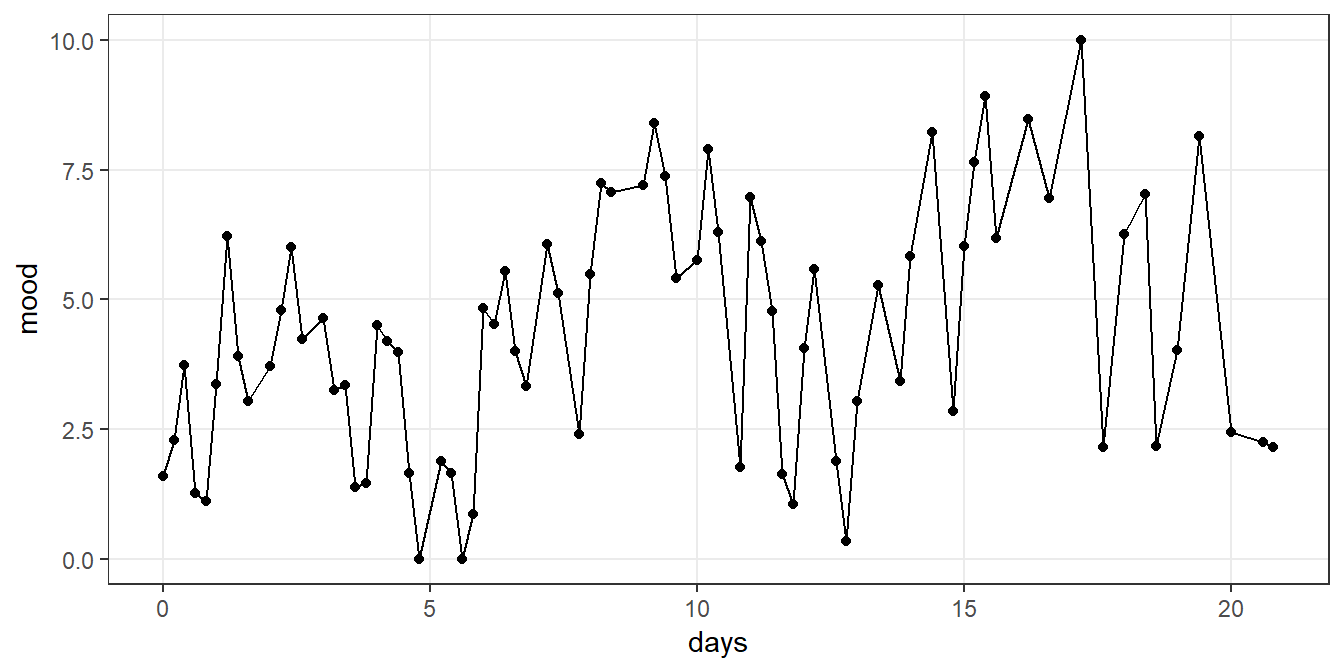
\includegraphics[width=1\linewidth]{features_files/figure-latex/feat-plot-1} 

}

\caption{A simulated three-week time-series of EMA mood ratings.}\label{fig:feat-plot}
\end{figure}

\section{Central Tendency and
Variability}\label{central-tendency-and-variability}

\index{Central tendency} \index{Central Variability}

Features do not necessarily have to be complex. Familiar measures of
central tendency of EMA time-series, such as the mode or the mean, can
be useful predictors of traditional clinical assessments. Standard
measures of the variability of EMA scores, such as the standard
deviation (SD), have been shown to have diagnostic value \citep[see,
e.g.,][]{bowen2006}. You should not hesitate to consider these
statistics when they help you to answer your research question.

\index{Stationarity} You should check, though, whether the implicit
assumptions behind the statistics are correct. When you use the mean and
the standard deviation to summarize a time-series, you assume that the
data-generating process behind the series is stable over time - in
technical terms: that this process is \emph{stationary}
\citep{wikiStationary}. If this assumption is incorrect (i.e., if the
process is unstable or non-stationary), the mean and SD are biased
statistics.

Our simulated EMA time-series is non-stationary, as can be seen in
Figure \ref{fig:feat-plot-mean}. We observe a trend: the mood of the
person increases over time. EMA scores tend to be below the mean in the
beginning, and above the mean at the end. The overall mean (\emph{M} =
4.4) overestimates the EMA scores of the first week (\emph{M} = 3.3),
and underestimates the scores of the last week (\emph{M} = 5.5). If you
use the overall mean as a feature of the time-series in your analyses,
you ignore the mood improvements over the three-week period. In clinical
research, you would probably not want to miss this other important
feature.

When a trend exists in a series, the overall standard deviation is
overestimated, because of the extra variability that is introduced by
the changes of the mean. This can be checked by comparing the SD of the
full series to the SD of smaller parts. In our example, the overall SD
is 2.4. If we calculate the average of the SD of scores of each day,
however, the estimated SD is 1.8. If the additional variability
introduced by the trend is cancelled out, our estimate of variability
decreases considerably.

\begin{figure}

{\centering 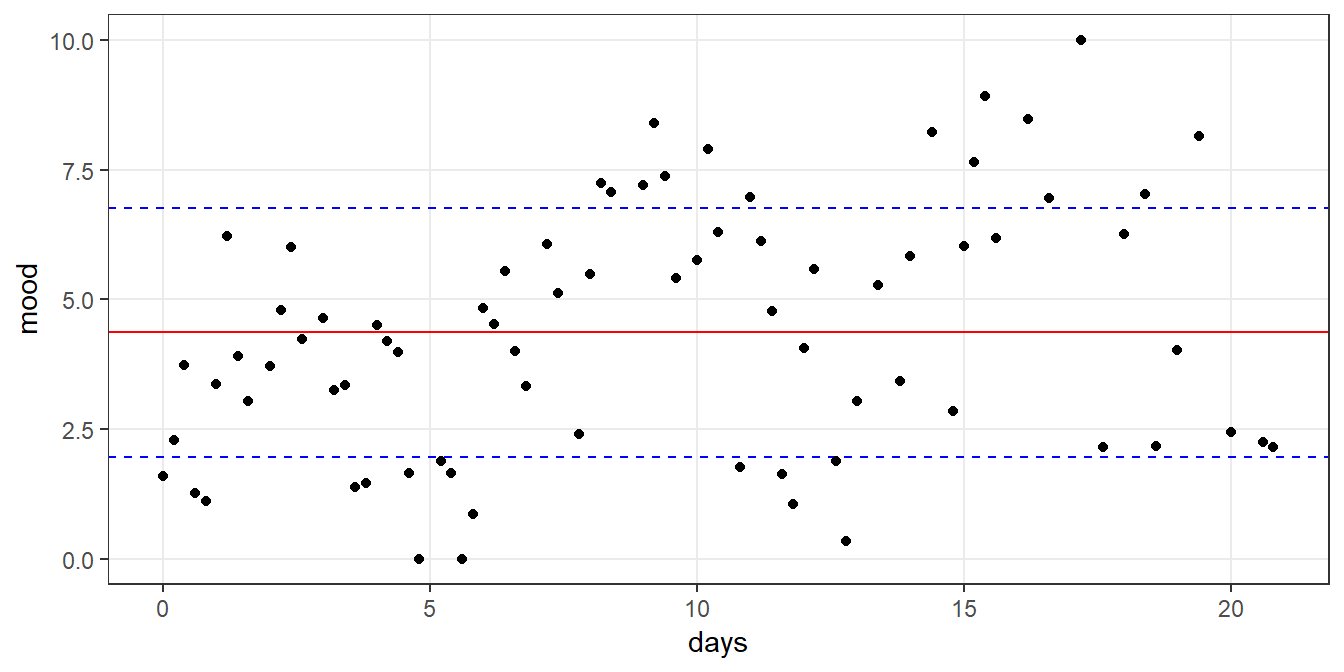
\includegraphics[width=1\linewidth]{features_files/figure-latex/feat-plot-mean-1} 

}

\caption{EMA time-series, with reference lines for the mean (red line) and the mean +/- 1 standard deviation range (the area between the two blue lines). Both statistics are informative, but obviously do not do full justice to the variation in observations over time.}\label{fig:feat-plot-mean}
\end{figure}

\section{Modelling the Trend}\label{modelling-the-trend}

Now that we know that the overall mean and SD are sub-optimal features
of this time-series, the question is how we can do better. What other
features can we extract? One option would be to characterize the series
in simple regression terms, via an intercept and a slope. By doing so,
we can economically describe the dynamics of the series with two
numbers. As can be seen in Figure \ref{fig:feat-plot-lm}, the regression
model provides a more realistic and informative summary. At the start,
the estimated mean - the intercept - is 3.2. This mean increases
approximately 0.9 points per week (the slope), to a final estimated mean
of 5.9. Comparing Figure \ref{fig:feat-plot-mean} and Figure
\ref{fig:feat-plot-lm}, we see that Figure \ref{fig:feat-plot-lm} is
more successful in capturing the variation in the series.

\begin{figure}

{\centering 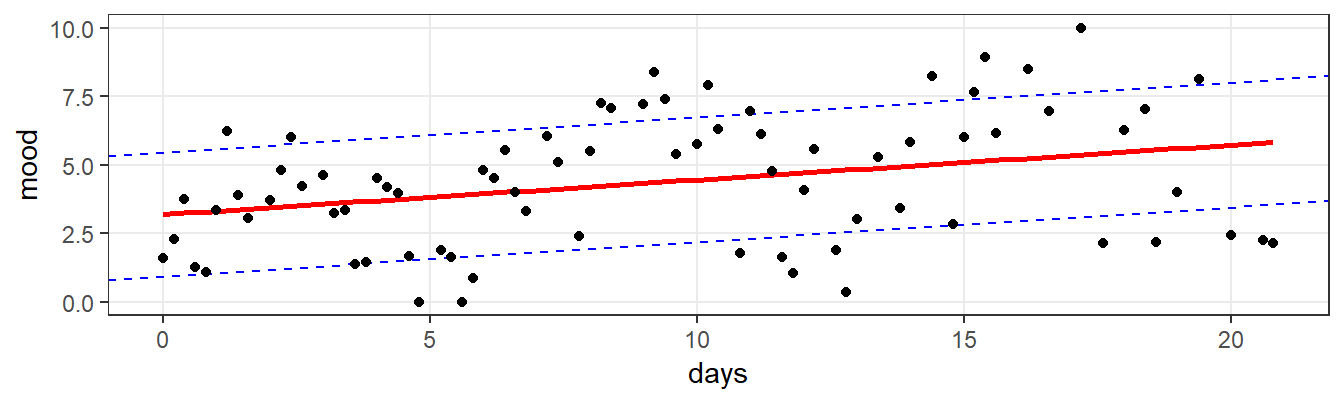
\includegraphics[width=1\linewidth]{features_files/figure-latex/feat-plot-lm-1} 

}

\caption{EMA time-series, with a regression reference line (red) and the residual error SD range around this line (the area between the two blue lines)}\label{fig:feat-plot-lm}
\end{figure}

By using regression, we can also find a better estimate of the SD.
Remember how the SD is conceptually defined as the average distance
between the scores and the mean. Since the mean is modeled by the
regression line, we can estimate the SD by calculating the standard
deviation of the residuals of the regression model that we used to
retrieve the intercept and slope. For our series, this results in an
estimated SD of 2.3. The new SD estimate is smaller than the overall SD,
as expected. By accounting for the extra variability introduced by the
trend, we get a more accurate estimate of the variability around the
mean at each point in time. However, the new estimate is still higher
than the daily estimate that we calculated above. Figure
\ref{fig:feat-plot-resid} provides a first indication of what is going
on. In the figure, absolution regression residuals are plotted over
time, with a regression line superposed. This reveals that residuals
increase as time goes by. We discovered a new feature of the series:
heteroscedasticity.

\begin{figure}

{\centering 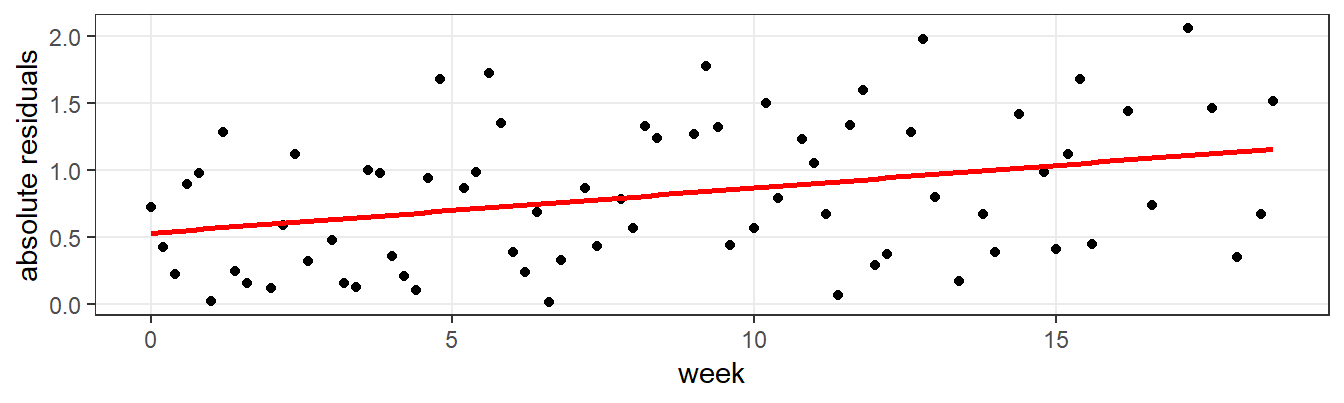
\includegraphics[width=1\linewidth]{features_files/figure-latex/feat-plot-resid-1} 

}

\caption{Plot of absolute regression residuals over time, revealing heteroscedasticity.}\label{fig:feat-plot-resid}
\end{figure}

\section{Missing Values}\label{missing-values}

\index{Missing values}

In EMA research, you should be prepared to deal with missing values.
Especially with active EMA, in which participants have to consciously
respond to prompted questions several times a day, non-response is
inevitable. Missing values are typically considered to be a nuisance
rather than a feature of EMA time-series. Non-response, however, is an
important characteristic, that may even have clinical relevance. Missing
values are also present in our simulated EMA time-series example, as you
may have found out already when you inspected Figure
\ref{fig:feat-plot}. The points, denoting the observed responses, are
denser in the beginning of the series. Over the course of the study
period, the probability of missed ratings increases. This becomes
immediately clear from Figure \ref{fig:feat-plot-na}, in which the
percentage of missed ratings is plotted per day. Every week, the
probability of missed ratings increases approximately 16\%.

\begin{figure}

{\centering 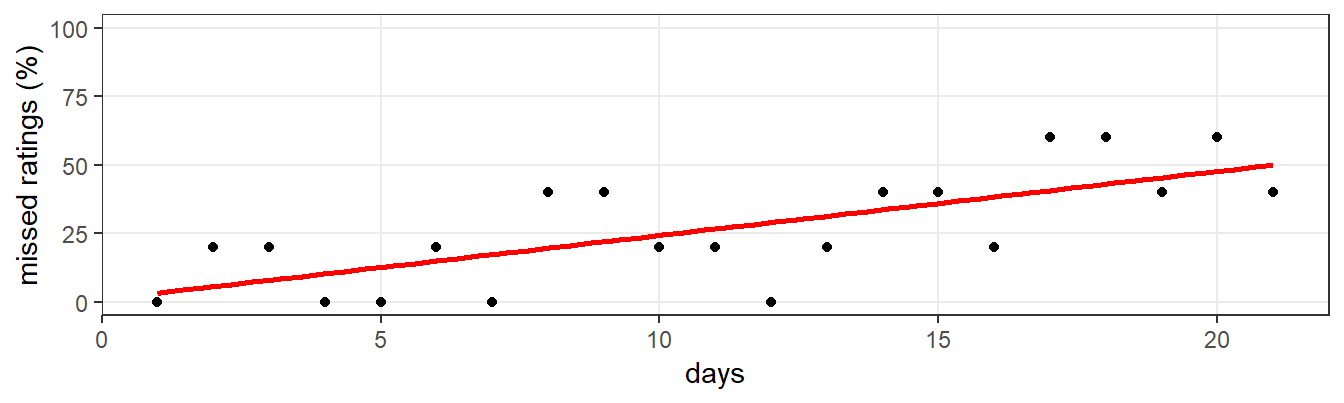
\includegraphics[width=1\linewidth]{features_files/figure-latex/feat-plot-na-1} 

}

\caption{Percentage of missed mood ratings, per day, over the three-week study period, with a regression line (red) superposed, revealing a familiar trend in EMA data.}\label{fig:feat-plot-na}
\end{figure}

Now that we now about these missing values, the question arises how to
deal with them? You can choose to ignore the missing values (assuming
that the occurrence of missing values was driven by a completely random
process). Alternatively, you could try to replace the missing values
with plausible values (in which case it becomes important to think about
the process that drives the missingness). If you decide to impute, there
are several options. For example, you can replace missing values with
the mean, the last-known value, an interpolated value or with a
smoothing technique such as the Kalman-filter \citep[see][for a
discussion]{hoogendoorn2017}. Figure \ref{fig:feat-plot-interpolation}
illustrates the linear interpolation approach: missing values (marked by
red dots) are replaced by values that lie between the non-missings.
Imagine that we would have used the mean to impute. Can you see why that
would have disrupted local patterns in the series?

\begin{figure}

{\centering 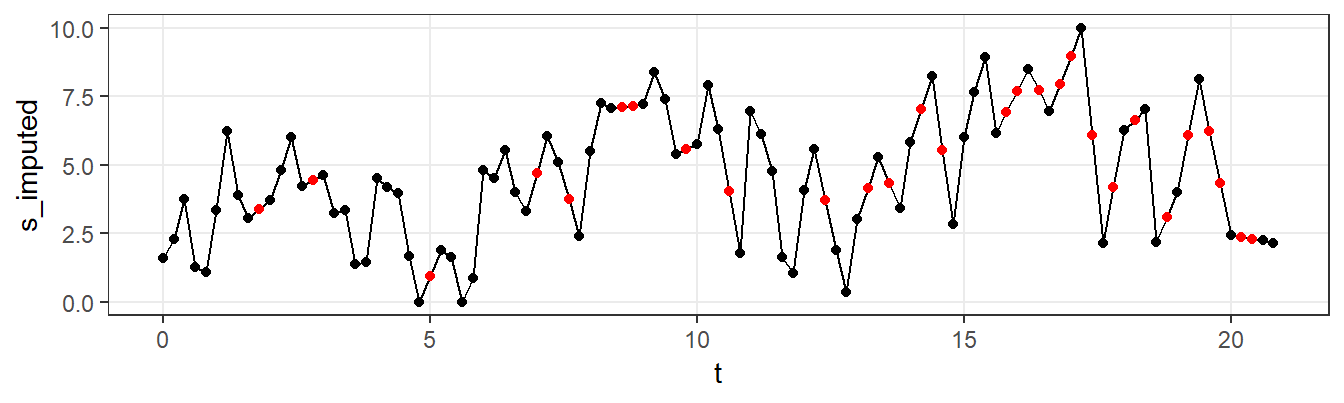
\includegraphics[width=1\linewidth]{features_files/figure-latex/feat-plot-interpolation-1} 

}

\caption{EMA time series, with missing values (red) imputed through interpolation.}\label{fig:feat-plot-interpolation}
\end{figure}

\section{Auto-correlation}\label{auto-correlation}

\index{Auto-correlation}

When a series is correlated with delayed copies of itself, we say that
it is auto-correlated. In repeated measurements of natural phenomena,
this auto-correlation can often be found. The temperature of today is
correlated with the temperature of recent days. Similarly, EMA mood
ratings, taken at time t, are typically correlated with ratings taken at
t-1, t-2, etc. Studying the auto-correlation of a time-series at
different delays can be very revealing, as illustrated by the
auto-correlation plot in Figure \ref{fig:feat-plot-autocorr}, in which
the correlation of the EMA series with itself is plotted, for various
delays (or `lags' as these delays are called). First, the plot reveals
that observations are correlated with previous values at lag 1: this
series is auto-correlated. Second, there appears to be a pattern in the
correlations at later lags: positive and negative correlations
alternate, in a pattern that seems to reflect periodicity.

\begin{figure}

{\centering 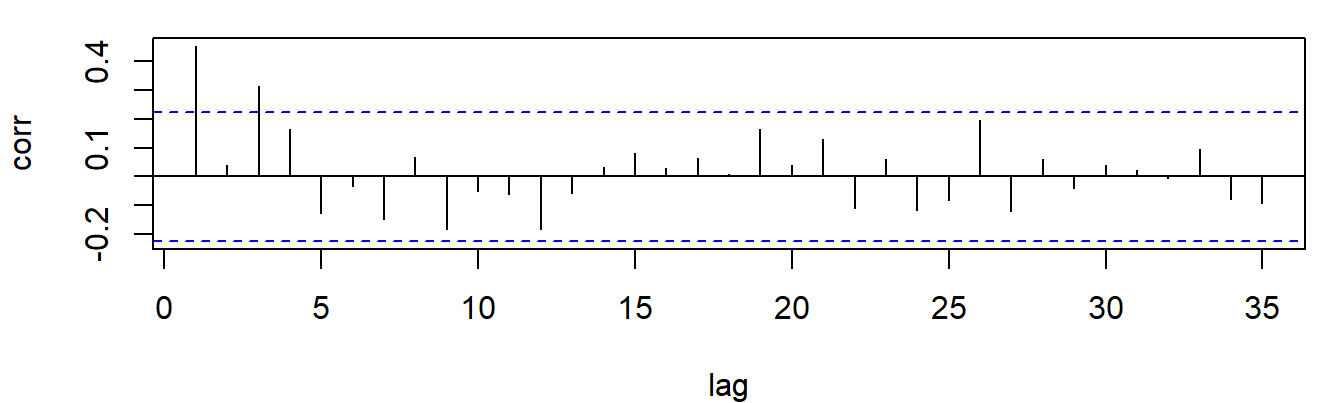
\includegraphics[width=1\linewidth]{features_files/figure-latex/feat-plot-autocorr-1} 

}

\caption{Autocorrelation plot of the EMA mood series, revealing periodicity.}\label{fig:feat-plot-autocorr}
\end{figure}

\subsection{Rolling Statistics}\label{rolling-statistics}

From the auto-correlation analysis, we learned that describing the EMA
series as a simple trend might be too simplistic. The mean does not
increase in a simple linear fashion. There seem to be periodic
components in the series as well: the signal appears also to be
characterized by a series of increases and decreases in the mean mood
level. In the plot of the raw series, this is not immediately clear.
However, if we ``smooth'' the series, by calculating the mean as it
develops over time, the periodicity in the series is becoming clearer.
Figure \ref{fig:feat-plot-roll} illustrates this.

\begin{figure}

{\centering 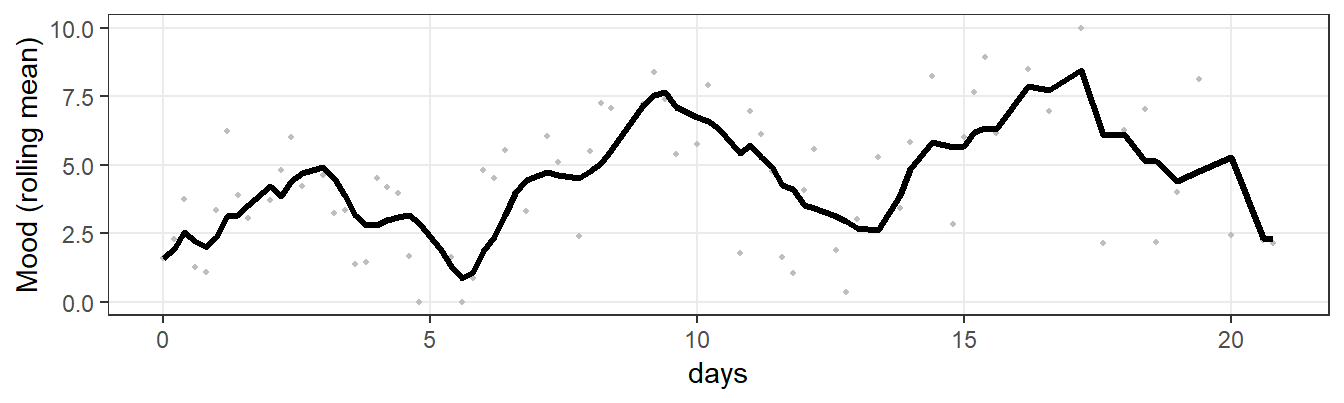
\includegraphics[width=1\linewidth]{features_files/figure-latex/feat-plot-roll-1} 

}

\caption{EMA mood series, with a rolling mean superposed.}\label{fig:feat-plot-roll}
\end{figure}

\section{Periodicity}\label{periodicity}

\index{Circadian rhythms}

Both the auto-correlation analysis and the moving average plot suggest
periodicity in the EMA time series. Suppose we want to know more about
this periodicity. Is there a way to quantify it? Yes, there is. With a
technique called Fourier Analysis, the strength (`power') of the
evidence for the presence of various frequencies can be quantified.
Figure \ref{fig:feat-plot-pow} shows what happens if we run a Fourier
analysis of our time series (with R's built-in function
\texttt{spec.pgram}).

\begin{figure}

{\centering 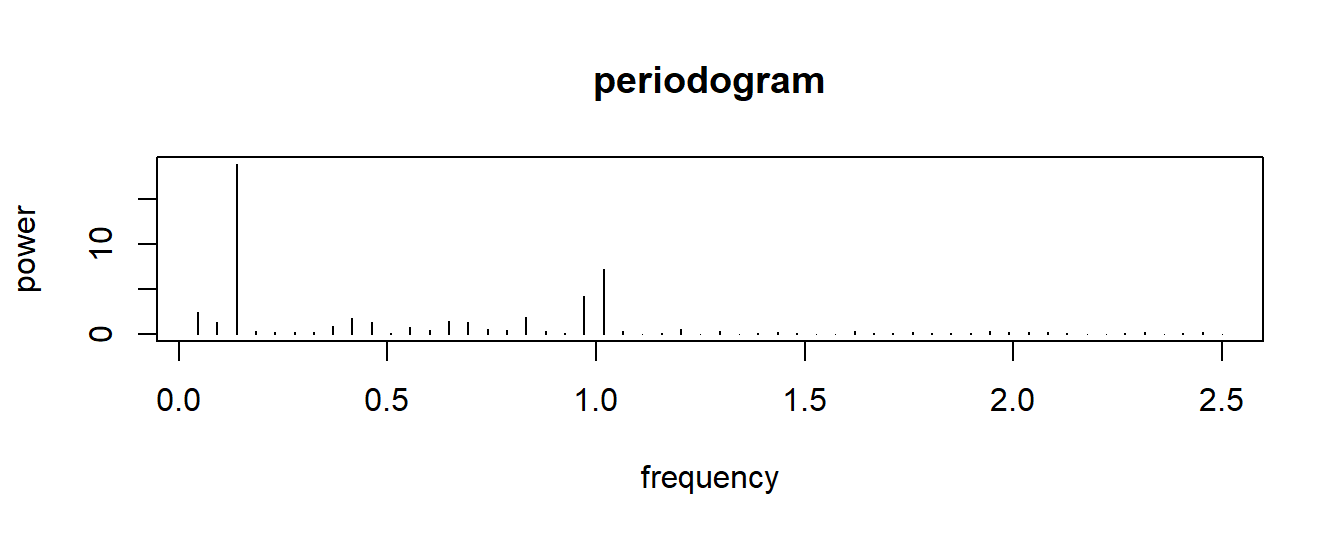
\includegraphics[width=1\linewidth]{features_files/figure-latex/feat-plot-pow-1} 

}

\caption{periodogram of the EMA time series, revealing a one-day and a one-week period.}\label{fig:feat-plot-pow}
\end{figure}

There are two peaks in the figure: at a frequency of 1 (day) and at a
frequency of 0.14 (about one week). This series is \emph{circadian}:
mood ratings follow a daily and a weekly pattern. This is a common
feature of EMA data, because of the circadian rhythms in our body and in
our environment (our biological clocks, day-night cycles, seasons)
\citep{Doherty2018, Frank2000, Frank2007, Karatsoreos2014, VanSomeren2000, Tahmasian2013}.

\section{Discussion}\label{discussion-1}

In this chapter, we used a number of statistical indicators to
characterize a single time-series. By extracting these indicators (or
``features''), we identified several regularities. We learned that the
mean, variance and missingness increased over time, and we identified
clear signs of circadian rhythmicity. You might have identified some of
these features when you first inspected Figure \ref{fig:feat-plot}. The
increase in the mean was pretty easy to spot. However, the systematic
increases in the variance and the missingness were less clear. Likewise,
although you might have spotted the periodicity in the series, the
circadian components were probably too subtle to spot for the naked eye.

The aim of the chapter was to illustrate the options available to the
EMA researcher to quantitatively summarize EMA series. Other options, of
course, exist. In chapter \ref{csd}, for example, we will see how subtle
changes in variation and auto-correlation in EMA mood scores can be
summarized in a single dynamic statistical feature that may be
predictive indicator of significant future state changes.

Finally, you might have been disappointed by the lack of code examples
in this chapter. We did not include them, to avoid unnecessary
distraction from the conceptual explanation. Instead, we provide a full
code listing below, to allow you learn how to apply the feature
extraction techniques yourself.

\index{Simulating data}

\begin{Shaded}
\begin{Highlighting}[]
\NormalTok{## (De)constructing a simulated EMA time-series}

\CommentTok{# libraries ----------------}
\KeywordTok{library}\NormalTok{(ggplot2)}
\KeywordTok{library}\NormalTok{(gridExtra)}
\KeywordTok{library}\NormalTok{(psych)}
\KeywordTok{library}\NormalTok{(zoo)}
\KeywordTok{library}\NormalTok{(emaph)}

\CommentTok{# simulate the signal (using emaph function) -------}
\NormalTok{d <-}\StringTok{ }\KeywordTok{generate_features_dataset}\NormalTok{(}\DataTypeTok{seed =} \DecValTok{123}\NormalTok{)}

\CommentTok{# plot -------------------------}
\NormalTok{e <-}\StringTok{ }\KeywordTok{subset}\NormalTok{(d,}\OperatorTok{!}\KeywordTok{is.na}\NormalTok{(s))}

\CommentTok{# raw series }
\KeywordTok{ggplot}\NormalTok{(e, }\KeywordTok{aes}\NormalTok{(}\DataTypeTok{x =}\NormalTok{ t, }\DataTypeTok{y =}\NormalTok{ s)) }\OperatorTok{+}
\StringTok{  }\KeywordTok{geom_line}\NormalTok{() }\OperatorTok{+}
\StringTok{  }\KeywordTok{geom_point}\NormalTok{() }\OperatorTok{+}
\StringTok{  }\KeywordTok{ylab}\NormalTok{(}\StringTok{"mood"}\NormalTok{) }\OperatorTok{+}\StringTok{ }\KeywordTok{xlab}\NormalTok{(}\StringTok{"days"}\NormalTok{) }\OperatorTok{+}
\StringTok{  }\KeywordTok{ylim}\NormalTok{(}\DecValTok{0}\NormalTok{, }\DecValTok{10}\NormalTok{) }\OperatorTok{+}
\StringTok{  }\KeywordTok{theme_bw}\NormalTok{() }\OperatorTok{+}\StringTok{ }\KeywordTok{theme}\NormalTok{(}\DataTypeTok{panel.grid.minor =} \KeywordTok{element_blank}\NormalTok{())}


\CommentTok{# plot mean and variance --------}
\KeywordTok{ggplot}\NormalTok{(e, }\KeywordTok{aes}\NormalTok{(}\DataTypeTok{x =}\NormalTok{ t, }\DataTypeTok{y =}\NormalTok{ s)) }\OperatorTok{+}
\StringTok{  }\KeywordTok{geom_hline}\NormalTok{(}\DataTypeTok{yintercept =} \KeywordTok{mean}\NormalTok{(e}\OperatorTok{$}\NormalTok{s, }\DataTypeTok{na.rm =} \OtherTok{TRUE}\NormalTok{), }\DataTypeTok{color =} \StringTok{"red"}\NormalTok{) }\OperatorTok{+}
\StringTok{  }\KeywordTok{geom_hline}\NormalTok{(}
    \DataTypeTok{yintercept =} \KeywordTok{mean}\NormalTok{(e}\OperatorTok{$}\NormalTok{s, }\DataTypeTok{na.rm =} \OtherTok{TRUE}\NormalTok{) }\OperatorTok{+}\StringTok{ }\KeywordTok{sd}\NormalTok{(e}\OperatorTok{$}\NormalTok{s, }\DataTypeTok{na.rm =} \OtherTok{TRUE}\NormalTok{),}
    \DataTypeTok{color =} \StringTok{"blue"}\NormalTok{,}
    \DataTypeTok{linetype =} \DecValTok{2}
\NormalTok{  ) }\OperatorTok{+}
\StringTok{  }\KeywordTok{geom_hline}\NormalTok{(}
    \DataTypeTok{yintercept =} \KeywordTok{mean}\NormalTok{(e}\OperatorTok{$}\NormalTok{s, }\DataTypeTok{na.rm =} \OtherTok{TRUE}\NormalTok{) }\OperatorTok{-}\StringTok{ }\KeywordTok{sd}\NormalTok{(e}\OperatorTok{$}\NormalTok{s, }\DataTypeTok{na.rm =} \OtherTok{TRUE}\NormalTok{),}
    \DataTypeTok{color =} \StringTok{"blue"}\NormalTok{,}
    \DataTypeTok{linetype =} \DecValTok{2}
\NormalTok{  ) }\OperatorTok{+}
\StringTok{  }\CommentTok{#geom_line() +}
\StringTok{  }\KeywordTok{geom_point}\NormalTok{() }\OperatorTok{+}
\StringTok{  }\KeywordTok{ylab}\NormalTok{(}\StringTok{"mood"}\NormalTok{) }\OperatorTok{+}\StringTok{ }\KeywordTok{xlab}\NormalTok{(}\StringTok{"days"}\NormalTok{) }\OperatorTok{+}
\StringTok{  }\KeywordTok{ylim}\NormalTok{(}\DecValTok{0}\NormalTok{, }\DecValTok{10}\NormalTok{) }\OperatorTok{+}
\StringTok{  }\KeywordTok{theme_bw}\NormalTok{() }\OperatorTok{+}\StringTok{ }\KeywordTok{theme}\NormalTok{(}\DataTypeTok{panel.grid.minor =} \KeywordTok{element_blank}\NormalTok{())}


\NormalTok{## The trends ---------------------}

\NormalTok{## run a linear regression of mood ratings by time}
\NormalTok{fm =}\StringTok{ }\KeywordTok{lm}\NormalTok{(s }\OperatorTok{~}\StringTok{ }\NormalTok{t, e)}

\NormalTok{## mean}
\KeywordTok{ggplot}\NormalTok{(e, }\KeywordTok{aes}\NormalTok{(}\DataTypeTok{x =}\NormalTok{ t, }\DataTypeTok{y =}\NormalTok{ s)) }\OperatorTok{+}
\StringTok{  }\KeywordTok{geom_smooth}\NormalTok{(}\DataTypeTok{method =} \StringTok{"lm"}\NormalTok{, }\DataTypeTok{color =} \StringTok{"red"}\NormalTok{, }\DataTypeTok{se =} \OtherTok{FALSE}\NormalTok{) }\OperatorTok{+}
\StringTok{  }\KeywordTok{geom_abline}\NormalTok{(}
    \DataTypeTok{intercept =} \KeywordTok{coef}\NormalTok{(fm)[}\DecValTok{1}\NormalTok{] }\OperatorTok{+}\StringTok{ }\KeywordTok{sd}\NormalTok{(}\KeywordTok{resid}\NormalTok{(fm)),}
    \DataTypeTok{slope =} \KeywordTok{coef}\NormalTok{(fm)[}\DecValTok{2}\NormalTok{],}
    \DataTypeTok{color =} \StringTok{"blue"}\NormalTok{,}
    \DataTypeTok{linetype =} \DecValTok{2}
\NormalTok{  ) }\OperatorTok{+}
\StringTok{  }\KeywordTok{geom_abline}\NormalTok{(}
    \DataTypeTok{intercept =} \KeywordTok{coef}\NormalTok{(fm)[}\DecValTok{1}\NormalTok{] }\OperatorTok{-}\StringTok{ }\KeywordTok{sd}\NormalTok{(}\KeywordTok{resid}\NormalTok{(fm)),}
    \DataTypeTok{slope =} \KeywordTok{coef}\NormalTok{(fm)[}\DecValTok{2}\NormalTok{],}
    \DataTypeTok{color =} \StringTok{"blue"}\NormalTok{,}
    \DataTypeTok{linetype =} \DecValTok{2}
\NormalTok{  ) }\OperatorTok{+}
\StringTok{  }\KeywordTok{geom_point}\NormalTok{() }\OperatorTok{+}
\StringTok{  }\KeywordTok{ylab}\NormalTok{(}\StringTok{"mood"}\NormalTok{) }\OperatorTok{+}\StringTok{ }\KeywordTok{xlab}\NormalTok{(}\StringTok{"days"}\NormalTok{) }\OperatorTok{+}
\StringTok{  }\KeywordTok{ylim}\NormalTok{(}\DecValTok{0}\NormalTok{, }\DecValTok{10}\NormalTok{) }\OperatorTok{+}
\StringTok{  }\KeywordTok{theme_bw}\NormalTok{() }\OperatorTok{+}\StringTok{ }\KeywordTok{theme}\NormalTok{(}\DataTypeTok{panel.grid.minor =} \KeywordTok{element_blank}\NormalTok{())}


\NormalTok{## residuals}
\NormalTok{e}\OperatorTok{$}\NormalTok{residuals <-}\StringTok{ }\KeywordTok{rstandard}\NormalTok{(fm)}
\NormalTok{e}\OperatorTok{$}\NormalTok{week <-}\StringTok{ }\NormalTok{(e}\OperatorTok{$}\NormalTok{t }\OperatorTok\StringTok{ }\DecValTok{1}\NormalTok{) }\OperatorTok{+}\StringTok{ }\DecValTok{1}

\KeywordTok{ggplot}\NormalTok{(}\KeywordTok{subset}\NormalTok{(e, week }\OperatorTok{<}\StringTok{ }\DecValTok{20}\NormalTok{), }\KeywordTok{aes}\NormalTok{(}\DataTypeTok{x =}\NormalTok{ t, }\DataTypeTok{y =} \KeywordTok{abs}\NormalTok{(residuals))) }\OperatorTok{+}
\StringTok{  }\KeywordTok{geom_point}\NormalTok{() }\OperatorTok{+}
\StringTok{  }\KeywordTok{geom_smooth}\NormalTok{(}\DataTypeTok{method =} \StringTok{"lm"}\NormalTok{, }\DataTypeTok{color =} \StringTok{"red"}\NormalTok{, }\DataTypeTok{se =} \OtherTok{FALSE}\NormalTok{) }\OperatorTok{+}
\StringTok{  }\KeywordTok{ylab}\NormalTok{(}\StringTok{"absolute residuals"}\NormalTok{) }\OperatorTok{+}\StringTok{ }\KeywordTok{xlab}\NormalTok{(}\StringTok{"week"}\NormalTok{) }\OperatorTok{+}
\StringTok{  }\KeywordTok{theme_bw}\NormalTok{() }\OperatorTok{+}\StringTok{ }\KeywordTok{theme}\NormalTok{(}\DataTypeTok{panel.grid.minor =} \KeywordTok{element_blank}\NormalTok{())}


\CommentTok{# Missing values ----------------------}

\NormalTok{d}\OperatorTok{$}\NormalTok{t_g <-}\StringTok{ }\KeywordTok{cut}\NormalTok{(t, }\DecValTok{21}\NormalTok{, }\DataTypeTok{labels =} \DecValTok{1}\OperatorTok{:}\DecValTok{21}\NormalTok{)}
\NormalTok{p <-}\StringTok{ }\KeywordTok{prop.table}\NormalTok{(}\KeywordTok{table}\NormalTok{(d}\OperatorTok{$}\NormalTok{t_g, }\KeywordTok{is.na}\NormalTok{(d}\OperatorTok{$}\NormalTok{s)), }\DecValTok{1}\NormalTok{)}
\NormalTok{p <-}\StringTok{ }\KeywordTok{as.data.frame}\NormalTok{(p)}
\NormalTok{p <-}\StringTok{ }\KeywordTok{subset}\NormalTok{(p, Var2 }\OperatorTok{==}\StringTok{ }\OtherTok{TRUE}\NormalTok{)}
\NormalTok{fm2 <-}\StringTok{ }\KeywordTok{lm}\NormalTok{(p}\OperatorTok{$}\NormalTok{Freq }\OperatorTok{~}\StringTok{ }\KeywordTok{as.numeric}\NormalTok{(p}\OperatorTok{$}\NormalTok{Var1))}

\KeywordTok{ggplot}\NormalTok{(p, }\KeywordTok{aes}\NormalTok{(}\DataTypeTok{x =} \KeywordTok{as.numeric}\NormalTok{(Var1), }\DataTypeTok{y =}\NormalTok{ Freq }\OperatorTok{*}\StringTok{ }\DecValTok{100}\NormalTok{)) }\OperatorTok{+}
\StringTok{  }\KeywordTok{geom_smooth}\NormalTok{(}\DataTypeTok{method =} \StringTok{"lm"}\NormalTok{, }\DataTypeTok{color =} \StringTok{"red"}\NormalTok{, }\DataTypeTok{se =} \OtherTok{FALSE}\NormalTok{) }\OperatorTok{+}
\StringTok{  }\KeywordTok{geom_point}\NormalTok{() }\OperatorTok{+}
\StringTok{  }\KeywordTok{ylab}\NormalTok{(}\StringTok{"missed ratings (%)"}\NormalTok{) }\OperatorTok{+}\StringTok{ }\KeywordTok{xlab}\NormalTok{(}\StringTok{"days"}\NormalTok{) }\OperatorTok{+}
\StringTok{  }\KeywordTok{ylim}\NormalTok{(}\DecValTok{0}\NormalTok{, }\DecValTok{100}\NormalTok{) }\OperatorTok{+}
\StringTok{  }\KeywordTok{theme_bw}\NormalTok{() }\OperatorTok{+}\StringTok{ }\KeywordTok{theme}\NormalTok{(}\DataTypeTok{panel.grid.minor =} \KeywordTok{element_blank}\NormalTok{())}


\NormalTok{## imputation through interpolation}
\NormalTok{impute_interpolation <-}\StringTok{ }\ControlFlowTok{function}\NormalTok{(x) \{}
  \KeywordTok{require}\NormalTok{(zoo)}
  
\NormalTok{  y =}\StringTok{ }\KeywordTok{zoo}\NormalTok{(x)}
  
  \CommentTok{# fill initial and trailing NA}
  \ControlFlowTok{if}\NormalTok{ (}\KeywordTok{is.na}\NormalTok{(y[}\DecValTok{1}\NormalTok{]))}
\NormalTok{    y[}\DecValTok{1}\NormalTok{] =}\StringTok{ }\NormalTok{y[}\KeywordTok{which.max}\NormalTok{(}\OperatorTok{!}\KeywordTok{is.na}\NormalTok{(y))]}
  \ControlFlowTok{if}\NormalTok{ (}\KeywordTok{is.na}\NormalTok{(y[}\KeywordTok{length}\NormalTok{(y)]))}
\NormalTok{    y[}\KeywordTok{length}\NormalTok{(y)] =}\StringTok{ }\NormalTok{y[}\KeywordTok{max}\NormalTok{((}\OperatorTok{!}\KeywordTok{is.na}\NormalTok{(y)) }\OperatorTok{*}\StringTok{ }\NormalTok{(}\DecValTok{1}\OperatorTok{:}\KeywordTok{length}\NormalTok{(y)))]}
  
  \CommentTok{# interpolate}
\NormalTok{  y_ =}\StringTok{ }\KeywordTok{as.numeric}\NormalTok{(}\KeywordTok{na.approx}\NormalTok{(y))}
  
\NormalTok{  y_}
\NormalTok{\}}


\NormalTok{d}\OperatorTok{$}\NormalTok{s_imputed <-}\StringTok{ }\KeywordTok{impute_interpolation}\NormalTok{(d}\OperatorTok{$}\NormalTok{s)}
\KeywordTok{ggplot}\NormalTok{(d, }\KeywordTok{aes}\NormalTok{(}\DataTypeTok{x =}\NormalTok{ t, }\DataTypeTok{y =}\NormalTok{ s_imputed)) }\OperatorTok{+}
\StringTok{  }\KeywordTok{geom_line}\NormalTok{(}\DataTypeTok{color =} \DecValTok{1}\NormalTok{) }\OperatorTok{+}
\StringTok{  }\KeywordTok{geom_point}\NormalTok{(}\KeywordTok{aes}\NormalTok{(}\DataTypeTok{color =} \KeywordTok{is.na}\NormalTok{(s))) }\OperatorTok{+}
\StringTok{  }\KeywordTok{scale_color_manual}\NormalTok{(}\DataTypeTok{values =} \KeywordTok{c}\NormalTok{(}\StringTok{"black"}\NormalTok{, }\StringTok{"red"}\NormalTok{)) }\OperatorTok{+}
\StringTok{  }\KeywordTok{guides}\NormalTok{(}\DataTypeTok{color =} \OtherTok{FALSE}\NormalTok{) }\OperatorTok{+}
\StringTok{  }\KeywordTok{theme_bw}\NormalTok{() }\OperatorTok{+}\StringTok{ }\KeywordTok{theme}\NormalTok{(}\DataTypeTok{panel.grid.minor =} \KeywordTok{element_blank}\NormalTok{())}


\CommentTok{# Autocorrelation ---------------------------}
\KeywordTok{acf}\NormalTok{(e}\OperatorTok{$}\NormalTok{s,}
    \DataTypeTok{type =} \StringTok{"partial"}\NormalTok{,}
    \DataTypeTok{lag.max =} \DecValTok{35}\NormalTok{,}
    \DataTypeTok{main =} \StringTok{""}\NormalTok{)}


\CommentTok{# Rolling mean ------------------------------}
\NormalTok{d}\OperatorTok{$}\NormalTok{rolling_mean <-}
\StringTok{  }\KeywordTok{as.numeric}\NormalTok{(}
\NormalTok{    zoo}\OperatorTok{::}\KeywordTok{rollapply}\NormalTok{(}
      \KeywordTok{as.numeric}\NormalTok{(d}\OperatorTok{$}\NormalTok{s),}
      \DataTypeTok{width =} \DecValTok{5}\NormalTok{,}
      \DataTypeTok{FUN =} \ControlFlowTok{function}\NormalTok{(x)}
        \KeywordTok{mean}\NormalTok{(x, }\DataTypeTok{na.rm =} \OtherTok{TRUE}\NormalTok{),}
      \DataTypeTok{fill =} \OtherTok{NA}\NormalTok{,}
      \DataTypeTok{align =} \StringTok{"right"}\NormalTok{,}
      \DataTypeTok{partial =} \OtherTok{TRUE}
\NormalTok{    )}
\NormalTok{  )}

\NormalTok{e <-}\StringTok{ }\KeywordTok{subset}\NormalTok{(d,}\OperatorTok{!}\KeywordTok{is.na}\NormalTok{(s))}
\KeywordTok{ggplot}\NormalTok{(e, }\KeywordTok{aes}\NormalTok{(}\DataTypeTok{x =}\NormalTok{ t, }\DataTypeTok{y =}\NormalTok{ rolling_mean)) }\OperatorTok{+}
\StringTok{  }\KeywordTok{geom_point}\NormalTok{(}\KeywordTok{aes}\NormalTok{(}\DataTypeTok{y =}\NormalTok{ s), }\DataTypeTok{color =} \StringTok{"grey"}\NormalTok{, }\DataTypeTok{size =}\NormalTok{ .}\DecValTok{8}\NormalTok{) }\OperatorTok{+}
\StringTok{  }\KeywordTok{geom_line}\NormalTok{(}\DataTypeTok{size =} \FloatTok{1.2}\NormalTok{) }\OperatorTok{+}
\StringTok{  }\KeywordTok{ylab}\NormalTok{(}\StringTok{"Mood (rolling mean)"}\NormalTok{) }\OperatorTok{+}\StringTok{ }\KeywordTok{xlab}\NormalTok{(}\StringTok{"days"}\NormalTok{) }\OperatorTok{+}
\StringTok{  }\KeywordTok{ylim}\NormalTok{(}\DecValTok{0}\NormalTok{, }\DecValTok{10}\NormalTok{) }\OperatorTok{+}
\StringTok{  }\KeywordTok{theme_bw}\NormalTok{() }\OperatorTok{+}\StringTok{ }\KeywordTok{theme}\NormalTok{(}\DataTypeTok{panel.grid.minor =} \KeywordTok{element_blank}\NormalTok{())}


\CommentTok{# Frequency analysis --------------------------}

\NormalTok{fa <-}
\StringTok{  }\KeywordTok{spec.pgram}\NormalTok{(}
    \KeywordTok{ts}\NormalTok{(}\KeywordTok{impute_interpolation}\NormalTok{(d}\OperatorTok{$}\NormalTok{s), }\DataTypeTok{frequency =}\NormalTok{ n_measurements_per_day),}
    \DataTypeTok{detrend =} \OtherTok{TRUE}\NormalTok{,}
    \DataTypeTok{demean =} \OtherTok{TRUE}\NormalTok{,}
    \DataTypeTok{main =} \StringTok{"periodogram"}\NormalTok{,}
    \DataTypeTok{sub =} \StringTok{""}\NormalTok{,}
    \DataTypeTok{xlab =} \StringTok{"frequency"}\NormalTok{,}
    \DataTypeTok{log =} \StringTok{"no"}\NormalTok{,}
    \DataTypeTok{ylab =} \StringTok{"power"}\NormalTok{,}
    \DataTypeTok{type =} \StringTok{"h"}\NormalTok{,}
    \DataTypeTok{spans =} \OtherTok{NULL}\NormalTok{,}
    \DataTypeTok{taper =} \FloatTok{0.01}\NormalTok{,}
    \DataTypeTok{ci =} \OtherTok{FALSE}
\NormalTok{  )}
\end{Highlighting}
\end{Shaded}

\chapter{Mixed Modeling}\label{lmm}

\index{Mixed Modeling}

EMA data are time-series that are characterized by complex correlational
structures, irregular sampling intervals, missing data, and substantive
individual differences. Mixed models are well-suited to deal with these
data. This chapter provides a brief introduction to conducting mixed
model analysis of EMA data in R.

\section{The Mixed Model}\label{the-mixed-model}

\index{Fixed effects} \index{Random effects}

Mixed modeling can be understood as a regression technique in which
separate regression functions are estimated for each cluster in the data
set. In EMA data, these clusters are defined by the participants. Data
from the same participant are expected to be correlated, and one way to
honor this correlation is to conceptualize a separate regression for
each participant. This idea, in the simplest regression model, can be
expressed as:

\begin{equation} 
  Y_{ij} = intercept_{i} + \epsilon_{ij} 
\end{equation}

This models the expected value of the j-th measurement of participant i
as the mean of all measurements of participant i, plus error. It defines
a set of regression functions - one for each participant. The regression
functions are, however, not independent. Mixed models divide the
intercepts of the individual participant regression functions into two
components: 1) the intercept of the group
(\emph{intercept\textsubscript{g}}; the mean intercept of all regression
functions), and 2) a participant-specific component
\emph{intercept\textsubscript{p}} (i.e., the difference between the
intercept of the participant and the mean intercept), i.e.:

\begin{equation} 
  intercept_{i} = intercept_{g} + intercept_{p} 
\end{equation}

The group intercept is called the `fixed' effect. If we would gather
more data from new participants, we would expect to find approximately
the same group intercept. The participant-specific component of the
intercept is known as the `random' effect. If we sample new data, we
would expect a similar \emph{variance} of the participant-specific
intercept components around the group intercept. This ``mixing'' of
fixed and random effects is what gives mixed modeling its name.

\section{Simulating Example Data}\label{simulating-example-data}

\index{Simulating data}

To understand analysis techniques, it often helps to apply the technique
to simulated data, in which parameters of interest are known. Here, we
will use the \texttt{sim\_ema} function from package \texttt{emaph}, to
simulate EMA mood assessments of 100 participants, who rate their mood,
three times per day, for one week. As you can learn from the
documentation of \texttt{sim\_ema} (see \texttt{?sim\_ema}), the
function expects at least two arguments: the definition of a sample plan
(see \texttt{?sample\_plan}), and a specification of the data-generating
model, in the form of a list defining fixed effects, the random effects,
and residual variance (i.e, the error).

\begin{Shaded}
\begin{Highlighting}[]
\CommentTok{# Simulating ema data.}
\KeywordTok{library}\NormalTok{(emaph)}
\NormalTok{plan <-}\StringTok{ }\KeywordTok{sample_plan}\NormalTok{(}\DataTypeTok{n_participants =} \DecValTok{100}\NormalTok{, }
                    \DataTypeTok{n_days =} \DecValTok{7}\NormalTok{,}
                    \DataTypeTok{times =} \KeywordTok{c}\NormalTok{(}\StringTok{"10:00-11:00"}\NormalTok{, }
                              \StringTok{"13:00-14:00"}\NormalTok{, }
                              \StringTok{"16:00-18:00"}\NormalTok{))}

\NormalTok{d1 <-}\StringTok{ }\KeywordTok{sim_ema}\NormalTok{(plan, }
              \DataTypeTok{mm_par =} \KeywordTok{list}\NormalTok{(}\DataTypeTok{fixed  =} \KeywordTok{c}\NormalTok{(}\DataTypeTok{intercept =} \DecValTok{5}\NormalTok{),}
                            \DataTypeTok{random =} \KeywordTok{c}\NormalTok{(}\DataTypeTok{intercept =} \DecValTok{1}\NormalTok{),}
                            \DataTypeTok{error =}\NormalTok{ .}\DecValTok{5}\NormalTok{),}
              \DataTypeTok{lim =} \KeywordTok{c}\NormalTok{(}\DecValTok{0}\NormalTok{, }\DecValTok{10}\NormalTok{))}
\end{Highlighting}
\end{Shaded}

From the code, you learn that we set the mean mood
(intercept\textsubscript{g}) to 5, the variance around this mean -
var(intercept\textsubscript{p}) - to 1, and the variance around these
means within participants - the error - to .5. Figure \ref{fig:lmm-plot}
shows EMA mood ratings of the first 6 participants in the simulated data
set, which we can use to check the simulation. As specified, mean mood
ratings of the participants (the red lines) vary around 5 (the grey
dashed line). So far, so good.

\begin{figure}

{\centering 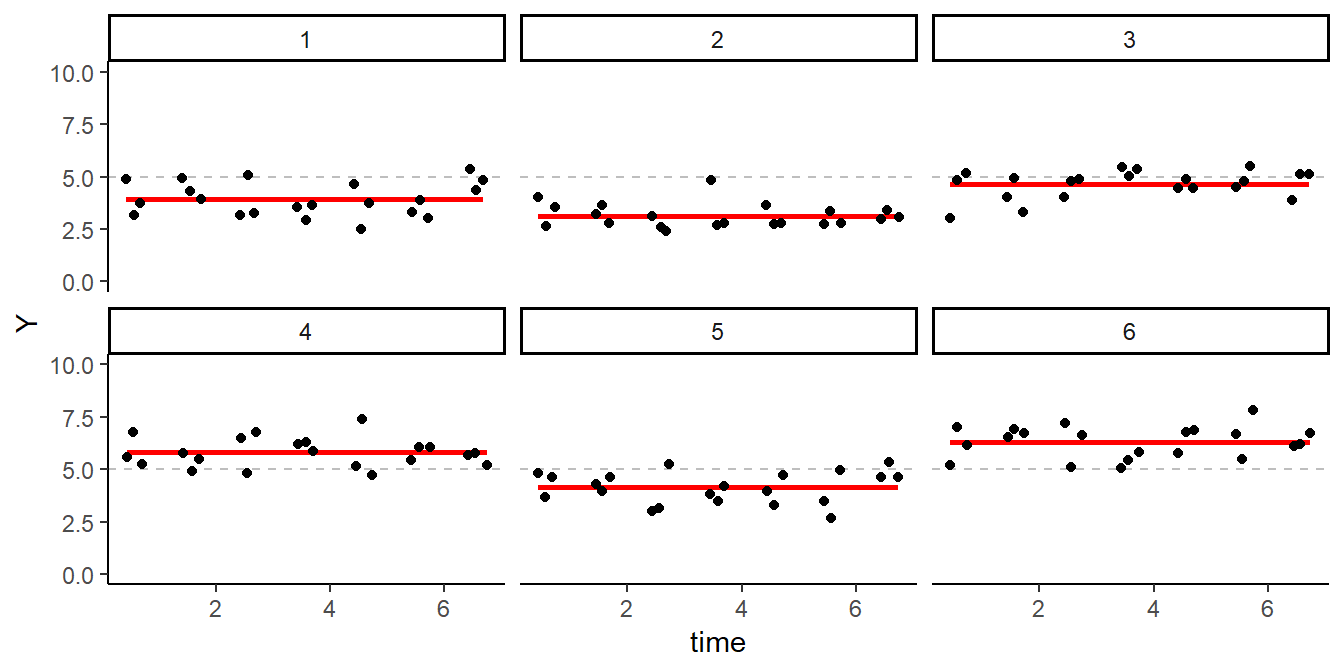
\includegraphics[width=1\linewidth]{lmm_files/figure-latex/lmm-plot-1} 

}

\caption{Simulated EMA data of Six Participants.}\label{fig:lmm-plot}
\end{figure}

\section{Fitting a Mixed Model in R}\label{fitting-a-mixed-model-in-r}

\index{nlme}

Now, let's fit a mixed model to the data, to see whether the simulation
parameters are detected. For this, we will use the \texttt{lme}
function, from package \texttt{nlme} \citep{R-nlme}. The code snippet
below shows how to do this.

The first argument of the lme function,
\texttt{Y\ \textasciitilde{}\ 1}, specifies the fixed `effect' (in this
case: the mean intercept). The second argument,
\texttt{random\ =\textasciitilde{}\ 1\ \textbar{}\ id} specifies the
random effect. In this model, intercepts are allowed to vary between
participants. The fitted model is assigned to a variable (\texttt{fm}),
which we will use later to study the fitted model.

\begin{Shaded}
\begin{Highlighting}[]
\CommentTok{# Fitting a mixed model with lme.}
\KeywordTok{library}\NormalTok{(nlme)}
\NormalTok{fm <-}\StringTok{ }\KeywordTok{lme}\NormalTok{(Y }\OperatorTok{~}\StringTok{ }\DecValTok{1}\NormalTok{, }\DataTypeTok{random =} \OperatorTok{~}\StringTok{ }\DecValTok{1} \OperatorTok{|}\StringTok{ }\NormalTok{id, }
          \DataTypeTok{data =}\NormalTok{ d1)}
\end{Highlighting}
\end{Shaded}

We can now extract the fixed effects regression coefficients table, by
calling the \texttt{summary} function on the fitted model. The estimated
intercept should be around 5 (as this is a finite sample, we expect some
deviation):

\begin{Shaded}
\begin{Highlighting}[]
\CommentTok{# Fixed effects.}
\KeywordTok{summary}\NormalTok{(fm)}\OperatorTok{$}\NormalTok{tTable}
\CommentTok{#>             Value Std.Error   DF t-value   p-value}
\CommentTok{#> (Intercept)  4.95     0.106 2000    46.7 1.28e-322}
\end{Highlighting}
\end{Shaded}

Random effects and residual variance are shown by the \texttt{VarCorr}
function. Again, since we specified the data ourselves in this case, we
know the `true' value of these parameters: the random intercept variance
should be around 1 and the residual error variance should be close to
0.5.

\begin{Shaded}
\begin{Highlighting}[]
\CommentTok{# Random effects.}
\KeywordTok{VarCorr}\NormalTok{(fm)}
\CommentTok{#> id = pdLogChol(1) }
\CommentTok{#>             Variance StdDev}
\CommentTok{#> (Intercept) 1.097    1.048 }
\CommentTok{#> Residual    0.502    0.709}
\end{Highlighting}
\end{Shaded}

It can be instructive to plot the predicted values of the model, to make
clear how the model `thinks'. As shown by Figure
\ref{fig:lmm-lme1-plot}, the model predicts a series of straight lines,
one for each participant, that vary around 5 (the red line).

\begin{Shaded}
\begin{Highlighting}[]
\CommentTok{# Saving predicted values.}
\NormalTok{d1}\OperatorTok{$}\NormalTok{predicted <-}\StringTok{ }\KeywordTok{predict}\NormalTok{(fm)}
\end{Highlighting}
\end{Shaded}

\begin{figure}

{\centering 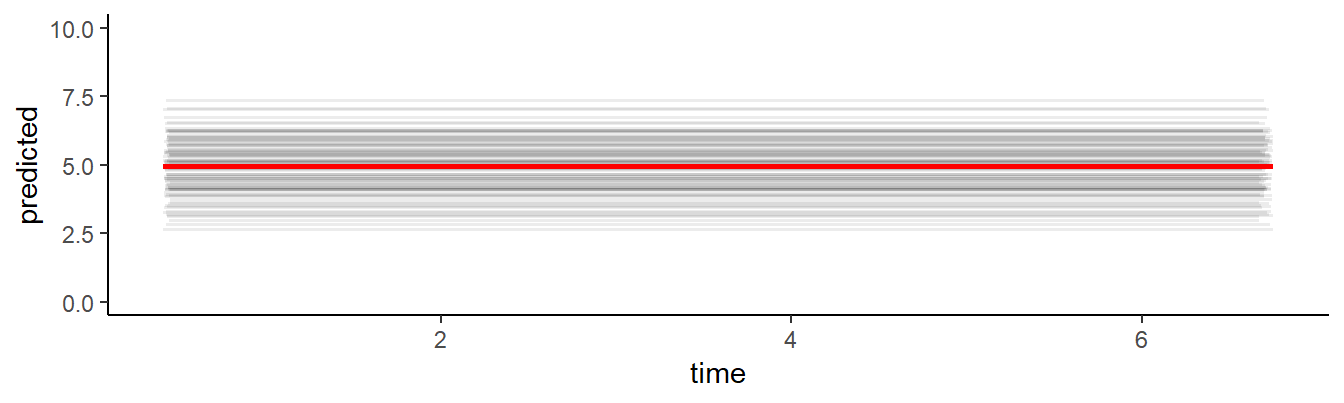
\includegraphics[width=1\linewidth]{lmm_files/figure-latex/lmm-lme1-plot-1} 

}

\caption{EMA ratings, of each participant in the simulated data set, as predicted by the intercept-only mixed linear model.}\label{fig:lmm-lme1-plot}
\end{figure}

\section{Adding Time as a Predictor}\label{adding-time-as-a-predictor}

Now that we know how to fit a simple mixed model, we can consider a more
complex scenario. In the first data set, participants' mood ratings did
not change over time. Scores varied around a stable mean during the full
week. Hence, there was no need to model a time effect. But suppose we
would expect a systematic improvement of mood ratings over time, for
instance in response to a mental health intervention?

Let's first call \texttt{sim\_ema} again, with parameters that will
result in data in which mood rating increase over the course of the
week, 0.5 scale points per day. Let's also assume that individual
participants will vary in the degree of mood improvement: the mean time
effect will be 0.5, but this parameter is allowed to vary between
participants, with a variance of 0.1.

\begin{Shaded}
\begin{Highlighting}[]
\CommentTok{# Simulating ema data (time effect).}
\NormalTok{d2 <-}\StringTok{ }\KeywordTok{sim_ema}\NormalTok{(plan, }
              \DataTypeTok{mm_par =} \KeywordTok{list}\NormalTok{(}\DataTypeTok{fixed  =} \KeywordTok{c}\NormalTok{(}\DataTypeTok{intercept =} \DecValTok{5}\NormalTok{, }\DataTypeTok{time =} \FloatTok{0.5}\NormalTok{),}
                            \DataTypeTok{random =} \KeywordTok{c}\NormalTok{(}\DataTypeTok{intercept =} \DecValTok{1}\NormalTok{, }\DataTypeTok{time =} \FloatTok{0.1}\NormalTok{),}
                            \DataTypeTok{error =}\NormalTok{ .}\DecValTok{5}\NormalTok{),}
              \DataTypeTok{lim =} \KeywordTok{c}\NormalTok{(}\DecValTok{0}\NormalTok{, }\DecValTok{10}\NormalTok{))}
\end{Highlighting}
\end{Shaded}

Figure \ref{fig:lmm-plot2} shows the data of the first six participants
in the second data set. Both the intercept and the slope vary across the
participants. Some participants improve more over time, and others
improve less: the slope in this data set is a random effect.

\begin{figure}

{\centering 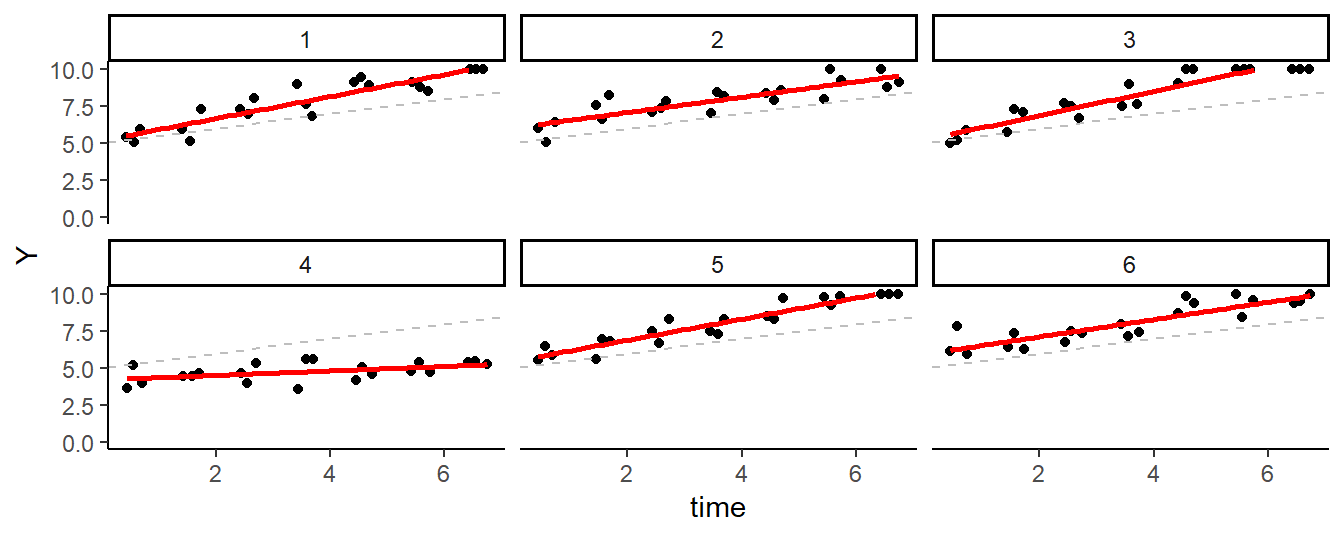
\includegraphics[width=1\linewidth]{lmm_files/figure-latex/lmm-plot2-1} 

}

\caption{Simulated EMA data of Six Participants (Time-varying model).}\label{fig:lmm-plot2}
\end{figure}

To fit the extended mixed model, time can simply be added to both the
fixed and random arguments of the `lme' function. Fixed effects
estimated of this model should be around 5 and 0.5, since that is how we
specified the data. Calling \texttt{summary} on this function, we see
that the fixed time effect is significant.

\begin{Shaded}
\begin{Highlighting}[]
\CommentTok{# A mixed model, with a random slope.}
\KeywordTok{library}\NormalTok{(nlme)}
\NormalTok{fm <-}\StringTok{ }\KeywordTok{lme}\NormalTok{(Y }\OperatorTok{~}\StringTok{ }\DecValTok{1} \OperatorTok{+}\StringTok{ }\NormalTok{time, }\DataTypeTok{random =} \OperatorTok{~}\StringTok{ }\DecValTok{1} \OperatorTok{+}\StringTok{ }\NormalTok{time }\OperatorTok{|}\StringTok{ }\NormalTok{id, }
          \DataTypeTok{data =}\NormalTok{ d2)}
\KeywordTok{summary}\NormalTok{(fm)}\OperatorTok{$}\NormalTok{tTable}
\CommentTok{#>             Value Std.Error   DF t-value   p-value}
\CommentTok{#> (Intercept) 5.112    0.1141 1999    44.8 4.94e-304}
\CommentTok{#> time        0.467    0.0263 1999    17.7  1.52e-65}
\end{Highlighting}
\end{Shaded}

The random effects now have four components: the variance of the
intercept, the variance of the slope, the residual error \emph{and} the
correlation between the random intercept and the random slope.

\begin{Shaded}
\begin{Highlighting}[]
\CommentTok{# Extracting random effects.}
\KeywordTok{VarCorr}\NormalTok{(fm)}
\CommentTok{#> id = pdLogChol(1 + time) }
\CommentTok{#>             Variance StdDev Corr  }
\CommentTok{#> (Intercept) 1.2071   1.099  (Intr)}
\CommentTok{#> time        0.0637   0.252  -0.231}
\CommentTok{#> Residual    0.4781   0.691}
\end{Highlighting}
\end{Shaded}

Model predictions clearly show how the mixed model estimated varying
intercepts and slopes, that, on average, approximate the fixed effect
regression formula \texttt{Y\ =\ 5\ +\ 0.5\ *\ time} that was used to
generate the data.

\begin{Shaded}
\begin{Highlighting}[]
\NormalTok{d2}\OperatorTok{$}\NormalTok{predicted <-}\StringTok{ }\KeywordTok{predict}\NormalTok{(fm)}

\KeywordTok{ggplot}\NormalTok{(d2, }\KeywordTok{aes}\NormalTok{(}\DataTypeTok{x =}\NormalTok{ time, }\DataTypeTok{y =}\NormalTok{ predicted, }\DataTypeTok{group =}\NormalTok{ id)) }\OperatorTok{+}\StringTok{ }
\StringTok{  }\KeywordTok{geom_line}\NormalTok{(}\DataTypeTok{alpha =}\NormalTok{ .}\DecValTok{1}\NormalTok{, }\DataTypeTok{size =}\NormalTok{ .}\DecValTok{6}\NormalTok{) }\OperatorTok{+}\StringTok{ }
\StringTok{  }\KeywordTok{geom_smooth}\NormalTok{(}\KeywordTok{aes}\NormalTok{(}\DataTypeTok{group =} \OtherTok{NULL}\NormalTok{), }\DataTypeTok{method =} \StringTok{"lm"}\NormalTok{, }\DataTypeTok{color =} \StringTok{"red"}\NormalTok{, }\DataTypeTok{size =} \FloatTok{1.2}\NormalTok{, }\DataTypeTok{linetype =} \DecValTok{2}\NormalTok{) }\OperatorTok{+}\StringTok{ }
\StringTok{  }\KeywordTok{coord_cartesian}\NormalTok{(}\DataTypeTok{ylim =} \KeywordTok{c}\NormalTok{(}\DecValTok{0}\NormalTok{, }\DecValTok{10}\NormalTok{)) }\OperatorTok{+}\StringTok{ }\KeywordTok{theme_classic}\NormalTok{()}
\end{Highlighting}
\end{Shaded}

\begin{center}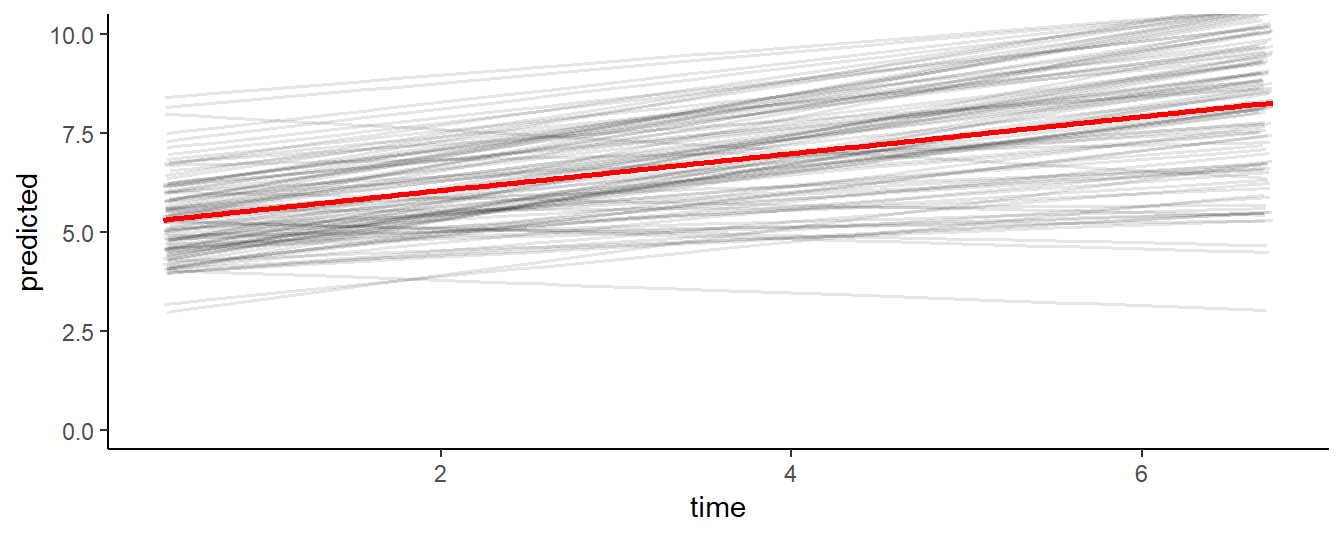
\includegraphics[width=1\linewidth]{lmm_files/figure-latex/lmm-lme2-pred-1} \end{center}

\section{Adding a Two-Group
Comparison}\label{adding-a-two-group-comparison}

In data-set 1, mood ratings did not change during the week, while in
data-set 2, the mood ratings increased. Suppose the two data-sets
reflect the data that you collect in a two-group RCT, in which you
compare the effects of a mental health intervention (data-set 2) against
a waiting list condition (data-set 1). By combining the two data-sets,
we can illustrate how to conduct a group comparison with \texttt{lme}.

Since the two data-sets are already available (in variables \texttt{d1}
and \texttt{d2}), the new data set can be created with just three lines
of code (below). In the first line, the \texttt{rbind} function is used
to combine the rows of data-set 1 and 2 into a new variable: d3. The
second line adds a group indicator to \texttt{d3}. The third line
updates the IDs of the participants in the second group, to
differentiate the participants in the second group from the participants
in the first group.

\begin{Shaded}
\begin{Highlighting}[]
\CommentTok{# Two-group simulation.}
\NormalTok{d3 <-}\StringTok{ }\KeywordTok{rbind}\NormalTok{(d1, d2)}
\NormalTok{d3}\OperatorTok{$}\NormalTok{group <-}\StringTok{ }\KeywordTok{factor}\NormalTok{(}\KeywordTok{c}\NormalTok{(}\KeywordTok{rep}\NormalTok{(}\DecValTok{0}\NormalTok{, }\KeywordTok{nrow}\NormalTok{(d1)), }\KeywordTok{rep}\NormalTok{(}\DecValTok{1}\NormalTok{, }\KeywordTok{nrow}\NormalTok{(d2))), }\DataTypeTok{labels =} \KeywordTok{c}\NormalTok{(}\StringTok{"control"}\NormalTok{, }\StringTok{"treatment"}\NormalTok{))}
\NormalTok{d3}\OperatorTok{$}\NormalTok{id[d3}\OperatorTok{$}\NormalTok{group }\OperatorTok{==}\StringTok{ "treatment"}\NormalTok{] <-}\StringTok{ }\NormalTok{d3}\OperatorTok{$}\NormalTok{id[d3}\OperatorTok{$}\NormalTok{group }\OperatorTok{==}\StringTok{ "treatment"}\NormalTok{] }\OperatorTok{+}\StringTok{ }\DecValTok{100}
\end{Highlighting}
\end{Shaded}

The effect of the intervention can be tested by adding a (fixed) `time *
group' interaction effect to the model. This effect, we know, is 0.5,
and, as can be seen, this is what the model picks up:

\begin{Shaded}
\begin{Highlighting}[]
\CommentTok{# A mixed model, with two groups.}
\KeywordTok{library}\NormalTok{(nlme)}
\NormalTok{fm <-}\StringTok{ }\KeywordTok{lme}\NormalTok{(Y }\OperatorTok{~}\StringTok{ }\DecValTok{1} \OperatorTok{+}\StringTok{ }\NormalTok{time }\OperatorTok{*}\StringTok{ }\NormalTok{group, }\DataTypeTok{random =} \OperatorTok{~}\StringTok{ }\DecValTok{1} \OperatorTok{+}\StringTok{ }\NormalTok{time }\OperatorTok{|}\StringTok{ }\NormalTok{id, }
          \DataTypeTok{data =}\NormalTok{ d3)}
\KeywordTok{round}\NormalTok{(}\KeywordTok{summary}\NormalTok{(fm)}\OperatorTok{$}\NormalTok{tTable, }\DecValTok{2}\NormalTok{)}
\CommentTok{#>                     Value Std.Error   DF t-value p-value}
\CommentTok{#> (Intercept)          4.93      0.11 3998   43.98    0.00}
\CommentTok{#> time                 0.00      0.02 3998    0.21    0.83}
\CommentTok{#> grouptreatment       0.18      0.16  198    1.14    0.25}
\CommentTok{#> time:grouptreatment  0.46      0.03 3998   16.71    0.00}
\end{Highlighting}
\end{Shaded}

In Figure \ref{fig:lmm-lme3-pred} below, EMA mood ratings predicted by
the fitted model show how the model detects 1) the fixed between-group
effect, and 2) the variance in intercepts and slopes in both groups.

\begin{figure}

{\centering 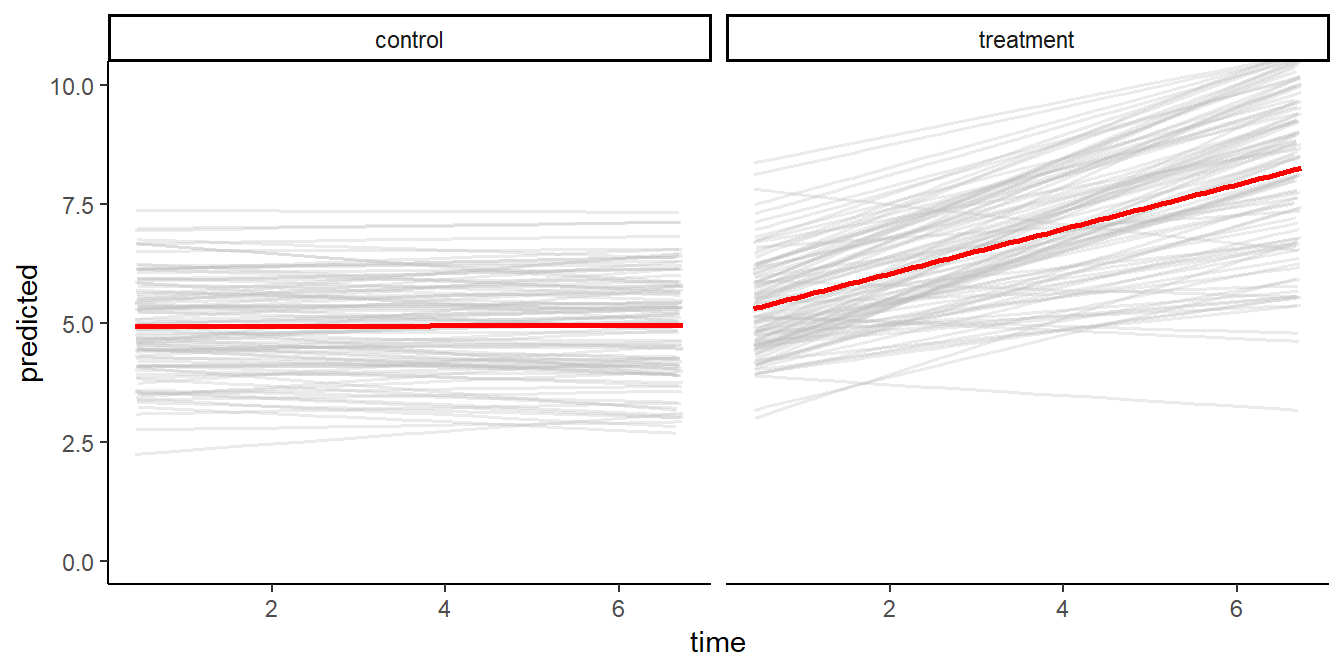
\includegraphics[width=1\linewidth]{lmm_files/figure-latex/lmm-lme3-pred-1} 

}

\caption{Predicted mood ratings}\label{fig:lmm-lme3-pred}
\end{figure}

\section{Next Steps}\label{next-steps}

In this chapter, we introduced mixed model analysis of EMA data in R. To
do so, we could only touch upon the theoretical foundations of mixed
models, and we deliberately used simple examples with clean simulated
data. Readers, who consider the application of mixed models, are
strongly advised to study additional resources.

The authoritative reference for mixed effect modeling in R is a book by
Pinheiro and Bates \citeyearpar{Pinheiro2000}. To fully appreciate this
book, however, a strong background in mathematical statistics is
required. Thorough introductions in the topic are further found in the
work of Prof.~dr. Jos Twisk \citep{twisk2006, twisk2013}, who also
teaches an applied mixed models course at the Department of Epidemiology
and Biostatistics at the Vrije Universiteit Medical Center (see:
\url{http://epidm.nl/en/courses/mixed-models/}).

\part{A Case Study}\label{part-a-case-study}

\chapter{Early Warning Signs of Depression}\label{csd}

One of the promises of EMA is that it might detect signs of mental
health deterioration in an early stage. Subtle changes in time series of
mood variables, for example, might signal a depression relapse. If we
can detect these changes, preventive interventions can be triggered to
avoid the relapse.

But what changes, exactly, should we look for? What are these early
warning signs?

\section{Critical Slowing Down}\label{critical-slowing-down}

\index{Critical Slowing Down}

Critical Slowing Down (CSD) is a concept from dynamic systems theory. In
dynamic systems, state transitions are preceded by a change in which the
system reacts to disturbances. In a stable state, the system quickly
recovers from disturbances. Prior to a transition to a new state,
however, the system takes more and more time to recover back to its
current state: the variance and auto-correlation of the system increases
\citep{Scheffer2009, Dakos2008}.

In this chapter, we re-analyze data from a study that aimed to
demonstrate CSD in EMA-data of a single patient with a history of major
depression \citetext{\citealp[
\citet{Kossakowski2017}]{Groot2010}; \citealp{Wichers2016}}. The
patient, a 57-year old male, used EMA to monitor himself during a
239-day single-case double-blind medication reduction trial. During the
experiment, he experienced a relapse, and Wichers and colleagues showed
how variance and auto-correlation in the EMA data increased, several
weeks prior to this relapse. The transition appeared to be preceded by
CSD.

We will try to reconstruct the finding, using an alternative analysis
strategy. One of the limitations of the Wichers et al analysis is that
auto-correlation was analyzed at lag 1 only (i.e., only the correlation
between t and t-1 was considered). With another analysis technique,
called `Detrended Fluctuation Analysis', all lags can be considered.

To conduct the analysis, we need three R packages: \index{tidyverse}
\index{nonlinearTseries} \index{empah}

\begin{itemize}
\item
  Raw EMA data of this study were published in the public domain
  \citep{Kossakowski2017}. We included the data in the \texttt{emaph}
  package.
\item
  To manipulate the raw data and reconstruct the plots of the article,
  we are going to use several functions from \texttt{tidyverse}
  packages.
\item
  DFA is implemented in package \texttt{nonlinearTseries}, so we will
  need that as well.
\end{itemize}

\begin{Shaded}
\begin{Highlighting}[]
\CommentTok{# Required libraries for the CSD-study re-analysis.}
\KeywordTok{library}\NormalTok{(emaph)}
\KeywordTok{library}\NormalTok{(tidyverse)}
\KeywordTok{library}\NormalTok{(nonlinearTseries)}
\end{Highlighting}
\end{Shaded}

\section{Plotting the Course of
Depression}\label{plotting-the-course-of-depression}

Let's take a look at the development of the depressive symptoms of the
patient first. These were tapped with weekly assessments of the
depression scale of the `Symptom Checklist-90-Revised'
\citep[SCL-90-R;][]{Derogatis1994}, a well-established self-report
questionnaire.

The code below reconstructs Figure 1 of the Wichers et al article. It
plots the SCL90-R depression scale score over the time. Around day 120,
the depression score increased considerable: the patient experienced a
relapse.

\begin{Shaded}
\begin{Highlighting}[]
\CommentTok{# Plot depression score.}
\NormalTok{dep <-}\StringTok{ }\NormalTok{csd }\OperatorTok\StringTok{ }\KeywordTok{select}\NormalTok{(dayno, scl90r_dep) }\OperatorTok
\StringTok{  }\KeywordTok{filter}\NormalTok{(}\OperatorTok{!}\KeywordTok{is.na}\NormalTok{(scl90r_dep)) }\OperatorTok\StringTok{ }\NormalTok{unique}

\CommentTok{# plot dep + change point (day 120 in our data)}
\KeywordTok{ggplot}\NormalTok{(dep, }\KeywordTok{aes}\NormalTok{(}\DataTypeTok{x =}\NormalTok{ dayno, }\DataTypeTok{y =}\NormalTok{ scl90r_dep, }\DataTypeTok{group =} \DecValTok{1}\NormalTok{)) }\OperatorTok{+}
\StringTok{  }\KeywordTok{geom_step}\NormalTok{() }\OperatorTok{+}
\StringTok{  }\KeywordTok{xlab}\NormalTok{(}\StringTok{"Days"}\NormalTok{) }\OperatorTok{+}\StringTok{ }\KeywordTok{ylab}\NormalTok{(}\StringTok{"SCL-90-R Depression"}\NormalTok{) }\OperatorTok{+}\StringTok{ }
\StringTok{  }\KeywordTok{theme_classic}\NormalTok{()}
\end{Highlighting}
\end{Shaded}

\begin{figure}

{\centering 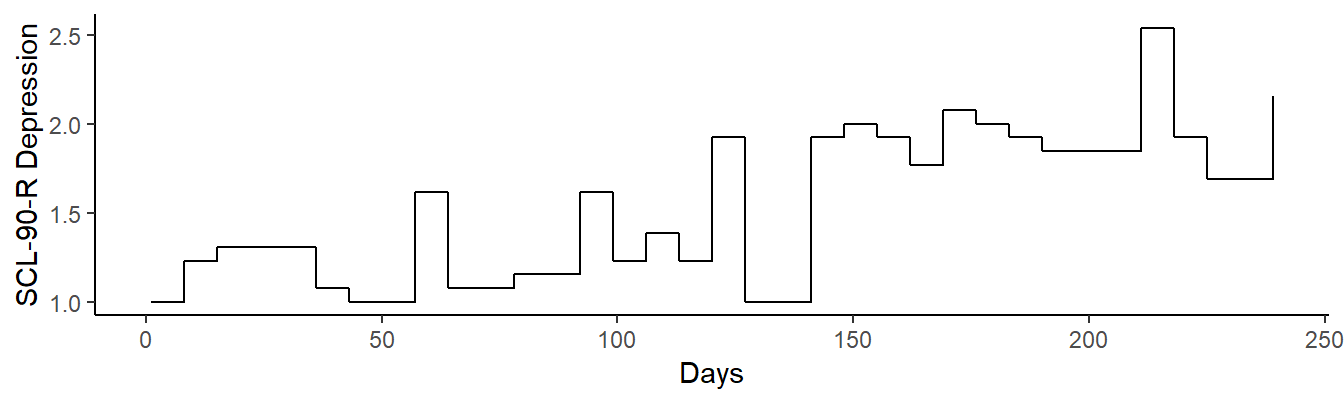
\includegraphics[width=1\linewidth]{csd_files/figure-latex/csd-scl90plot-1} 

}

\caption{SCL-90 depression score, over the study period}\label{fig:csd-scl90plot}
\end{figure}

\section{Mental state EMA Items}\label{mental-state-ema-items}

Wichers and colleagues selected 13 items from the full EMA data set,
which they grouped in 5 factors: positive affect (pa; 4 items), negative
affect (\texttt{na}; 4 items), mental unrest (\texttt{mu}; 3 items),
suspiciousness (\texttt{su}; 1 item), and worrying (\texttt{wo}; 1
item). From these factors, an overall mental state sum score can be
calculated.

\begin{Shaded}
\begin{Highlighting}[]
\CommentTok{# Mood states calculation.}

\CommentTok{# positive affect}
\NormalTok{pa_items <-}\StringTok{ }\KeywordTok{c}\NormalTok{(}\StringTok{"mood_enthus"}\NormalTok{, }\StringTok{"mood_cheerf"}\NormalTok{,}
              \StringTok{"mood_strong"}\NormalTok{, }\StringTok{"mood_satisfi"}\NormalTok{)}

\NormalTok{csd}\OperatorTok{$}\NormalTok{pa <-}\StringTok{ }\NormalTok{csd }\OperatorTok
\StringTok{  }\KeywordTok{select}\NormalTok{(pa_items) }\OperatorTok
\StringTok{  }\KeywordTok{rowMeans}\NormalTok{(., }\DataTypeTok{na.rm =} \OtherTok{TRUE}\NormalTok{)}
\NormalTok{csd}\OperatorTok{$}\NormalTok{pa <-}\StringTok{ }\OperatorTok{-}\NormalTok{csd}\OperatorTok{$}\NormalTok{pa}

\CommentTok{# negative affect}
\NormalTok{na_items <-}\StringTok{ }\KeywordTok{c}\NormalTok{(}\StringTok{"mood_lonely"}\NormalTok{, }\StringTok{"mood_anxious"}\NormalTok{,}
              \StringTok{"mood_guilty"}\NormalTok{, }\StringTok{"mood_doubt"}\NormalTok{)}

\NormalTok{csd}\OperatorTok{$}\NormalTok{na <-}\StringTok{ }\NormalTok{csd }\OperatorTok
\StringTok{  }\KeywordTok{select}\NormalTok{(na_items) }\OperatorTok
\StringTok{  }\KeywordTok{rowMeans}\NormalTok{(., }\DataTypeTok{na.rm =} \OtherTok{TRUE}\NormalTok{)}

\CommentTok{# mental unrest}
\NormalTok{mu_items <-}\StringTok{ }\KeywordTok{c}\NormalTok{(}\StringTok{"mood_irritat"}\NormalTok{, }\StringTok{"pat_restl"}\NormalTok{,}
              \StringTok{"pat_agitate"}\NormalTok{)}
\NormalTok{csd}\OperatorTok{$}\NormalTok{mu <-}\StringTok{ }\NormalTok{csd }\OperatorTok
\StringTok{  }\KeywordTok{select}\NormalTok{(mu_items) }\OperatorTok
\StringTok{  }\KeywordTok{rowMeans}\NormalTok{(., }\DataTypeTok{na.rm =} \OtherTok{TRUE}\NormalTok{)}

\CommentTok{# 'single-item' states}
\NormalTok{csd}\OperatorTok{$}\NormalTok{su <-}\StringTok{ }\NormalTok{csd}\OperatorTok{$}\NormalTok{mood_suspic}
\NormalTok{csd}\OperatorTok{$}\NormalTok{wo <-}\StringTok{ }\NormalTok{csd}\OperatorTok{$}\NormalTok{pat_worry}

\CommentTok{# global mental state score}
\NormalTok{csd}\OperatorTok{$}\NormalTok{ms <-}\StringTok{ }\KeywordTok{rowSums}\NormalTok{(csd[}\KeywordTok{c}\NormalTok{(}\StringTok{"pa"}\NormalTok{, }\StringTok{"na"}\NormalTok{, }\StringTok{"mu"}\NormalTok{, }\StringTok{"su"}\NormalTok{, }\StringTok{"wo"}\NormalTok{)])}
\end{Highlighting}
\end{Shaded}

Rows, in which one or more of the factors have missing values, are
removed from the analysis. In a full analysis, options to impute the
missing values could and should be considered. However, since only 3 of
the 1476 rows have missing item scores, not much is probably lost by
running a simple complete-case analysis.

\begin{Shaded}
\begin{Highlighting}[]
\CommentTok{# Missing values removal.}

\CommentTok{# count number of items with missing items, per row}
\NormalTok{csd}\OperatorTok{$}\NormalTok{nna <-}\StringTok{ }\NormalTok{csd }\OperatorTok
\StringTok{  }\KeywordTok{select}\NormalTok{(}\KeywordTok{matches}\NormalTok{(}\StringTok{"mood_"}\NormalTok{)) }\OperatorTok
\StringTok{  }\KeywordTok{is.na}\NormalTok{(.) }\OperatorTok\StringTok{ }\NormalTok{rowSums}

\CommentTok{# drop rows with missing values}
\NormalTok{csd <-}\StringTok{ }\NormalTok{csd }\OperatorTok\StringTok{ }\KeywordTok{filter}\NormalTok{(nna }\OperatorTok{==}\StringTok{ }\DecValTok{0}\NormalTok{)}
\end{Highlighting}
\end{Shaded}

\section{Running the DFA}\label{running-the-dfa}

\index{DFA analysis}

We are now ready to run the DFA analysis. We split the full series in
31-day overlapping windows, in steps of 1 day (i.e., day 1-31, day 2-32,
etc.), calculate the DFA of each window and save that value so that we
can compare it to the weekly depression assessments.

\begin{Shaded}
\begin{Highlighting}[]
\CommentTok{# Running the DFA.}

\CommentTok{# prepare result rows: one row for each day}
\NormalTok{d <-}\StringTok{ }\OtherTok{NULL}
\NormalTok{d <-}\StringTok{ }\NormalTok{csd }\OperatorTok\StringTok{ }
\StringTok{  }\KeywordTok{group_by}\NormalTok{(dayno) }\OperatorTok
\StringTok{  }\KeywordTok{summarise}\NormalTok{(}\DataTypeTok{ms =} \KeywordTok{mean}\NormalTok{(ms))}
\NormalTok{d}\OperatorTok{$}\NormalTok{ms_dfa =}\StringTok{ }\OtherTok{NA}

\CommentTok{# determine DFA, in a moving window of 31 days}
\NormalTok{window <-}\StringTok{ }\DecValTok{31}
\ControlFlowTok{for}\NormalTok{ (i }\ControlFlowTok{in} \KeywordTok{seq}\NormalTok{(window, }\KeywordTok{max}\NormalTok{(csd}\OperatorTok{$}\NormalTok{dayno), }\DecValTok{1}\NormalTok{)) \{}

  \CommentTok{# get the sliding window data}
\NormalTok{  w <-}\StringTok{ }\KeywordTok{subset}\NormalTok{(csd, dayno }\OperatorTok{>}\StringTok{ }\NormalTok{(i }\OperatorTok{-}\StringTok{ }\NormalTok{window) }\OperatorTok{&}\StringTok{ }\NormalTok{dayno }\OperatorTok{<=}\StringTok{ }\NormalTok{i)}

  \CommentTok{# dfa: ms}
\NormalTok{  dfa.analysis <-}\StringTok{ }\KeywordTok{dfa}\NormalTok{(}\DataTypeTok{time.series =}\NormalTok{ w}\OperatorTok{$}\NormalTok{ms,}
                      \DataTypeTok{npoints =} \DecValTok{30}\NormalTok{,}
                      \DataTypeTok{window.size.range =} \KeywordTok{c}\NormalTok{(}\DecValTok{10}\NormalTok{, }\KeywordTok{nrow}\NormalTok{(w)),}
                      \DataTypeTok{do.plot =} \OtherTok{FALSE}\NormalTok{)}

\NormalTok{  fgn.estimation <-}\StringTok{ }\KeywordTok{estimate}\NormalTok{(dfa.analysis,}
                            \DataTypeTok{do.plot =} \OtherTok{FALSE}\NormalTok{,}
                            \DataTypeTok{fit.col =} \StringTok{"blue"}\NormalTok{, }\DataTypeTok{fit.lwd =} \DecValTok{2}\NormalTok{, }\DataTypeTok{fit.lty =} \DecValTok{2}\NormalTok{,}
                            \DataTypeTok{main =} \StringTok{"Fitting DFA to fGn"}\NormalTok{)}
  
\NormalTok{  d}\OperatorTok{$}\NormalTok{ms_dfa[d}\OperatorTok{$}\NormalTok{dayno }\OperatorTok{==}\StringTok{ }\NormalTok{i] <-}\StringTok{ }\NormalTok{fgn.estimation}
\NormalTok{\}}
\end{Highlighting}
\end{Shaded}

\section{Results}\label{results}

We can now plot the DFA indicator over time, to see whether it peaks
prior to the onset of the relapse. As can be seen, the DFA-indicator
clearly peaks prior to the onset of the relapse, around day 110 (where
the color changes to red). Interestingly, a second peak is reached at
the end of the experiment, around day 239, indicating - perhaps - a
recovery from the relapse.

\begin{Shaded}
\begin{Highlighting}[]
\CommentTok{# Plot DFA results.}
\KeywordTok{ggplot}\NormalTok{(}\KeywordTok{na.omit}\NormalTok{(d),}
      \KeywordTok{aes}\NormalTok{(}\DataTypeTok{x =}\NormalTok{ dayno, }\DataTypeTok{y =}\NormalTok{ ms_dfa, }
          \DataTypeTok{colour =} \KeywordTok{factor}\NormalTok{(dayno }\OperatorTok{<}\StringTok{ }\DecValTok{120}\NormalTok{), }
          \DataTypeTok{group =} \DecValTok{1}\NormalTok{)) }\OperatorTok{+}
\StringTok{  }\KeywordTok{geom_point}\NormalTok{() }\OperatorTok{+}
\StringTok{  }\KeywordTok{geom_line}\NormalTok{() }\OperatorTok{+}\StringTok{ }
\StringTok{  }\KeywordTok{ylab}\NormalTok{(}\StringTok{"dfa (60-day window)"}\NormalTok{) }\OperatorTok{+}\StringTok{ }
\StringTok{  }\KeywordTok{xlim}\NormalTok{(}\KeywordTok{c}\NormalTok{(}\DecValTok{0}\NormalTok{, }\DecValTok{250}\NormalTok{)) }\OperatorTok{+}\StringTok{ }
\StringTok{  }\KeywordTok{guides}\NormalTok{(}\DataTypeTok{color =} \OtherTok{FALSE}\NormalTok{) }\OperatorTok{+}\StringTok{ }
\StringTok{  }\KeywordTok{theme_classic}\NormalTok{()}
\end{Highlighting}
\end{Shaded}

\begin{figure}

{\centering 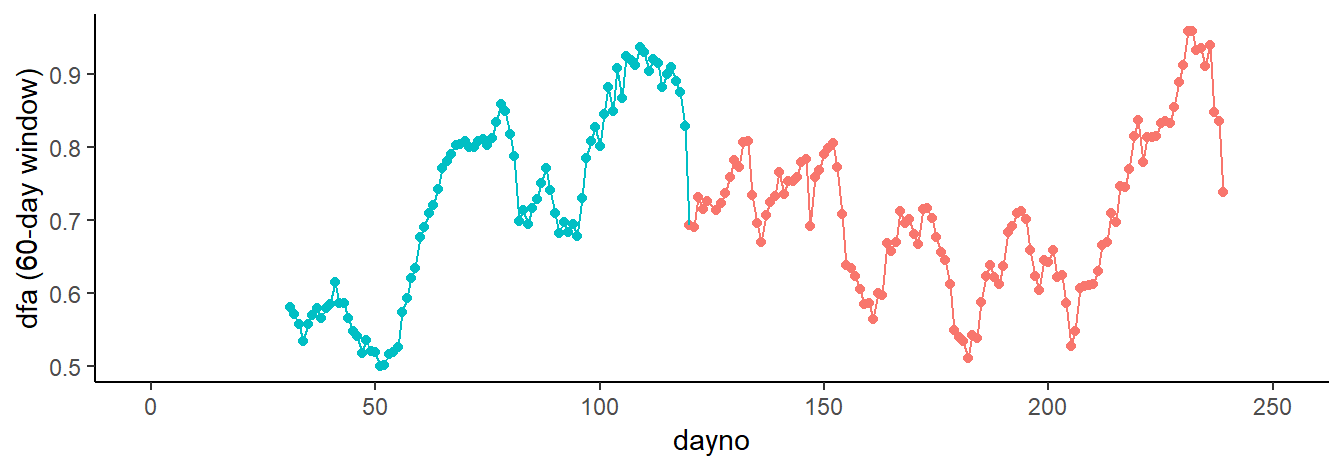
\includegraphics[width=1\linewidth]{csd_files/figure-latex/csd-dfaplot-1} 

}

\caption{Results of the DFA analysis.}\label{fig:csd-dfaplot}
\end{figure}

\section{Discussion}\label{discussion-2}

Our re-analysis replicates the main finding of the Wichers et al article
(\citep{Wichers2016}): several weeks prior to a depression relapse, as
predicted by complex systems theory, the variance and auto-correlation
in EMA mood ratings increased.

Potential clinical applications, of course, are clear. If clinically
relevant changes can be predicted algorithmically from EMA ratings,
automated patient feedback systems could help to prevent pending
deterioration or consolidate the path towards recovery.

One swallow, however, does not make summer. Yes, in this case, the
DFA-indicator peaked prior to the relapse. This could be a mere
coincidence. The predictive power of CSD needs to be confirmed in larger
samples and prospective studies. Given the theoretical background,
successful applications of CSD in other domains, and the present
finding, the spending of resources on such studies seems warranted.

Important additional questions remain to be answered. When it predicts a
state change, what is the expected delay between this prediction and the
change? Does a critical DFA-value exist? Given that critical value, are
false positive and false negative rates of this prediction acceptable?
These are important questions that should be answered before any
clinical application of DFA can be considered.

Re-analysis of data from completed clinical studies, in which EMA data
were collected, may be a first step to further explore the value of CSD.
One option, for example, would be to re-analyze data from the E-COMPARED
study \citep{Kleiboer2016}. In this trial, patients, who were treated
for major depression, completed weekly self-report questionnaires
\citep[the Patient Health Questionnaire; PHQ-8,][]{Kroenke2009} and
daily EMA mood ratings throughout treatment, which lasted up to 16-week.
Since CSD is an indicator of \emph{any} state change (i.e., irrespective
of whether the change is clinically ``good'' or ``bad''), theory would
predict a (lagged) relationship between CSD (i.e., the DFA-score) and
clinically significant changes in PHQ-scores \citep{Jacobson1991}.

\part{EMA Catalogues}\label{part-ema-catalogues}

\chapter{EMA Research within the APH Mental Health
Consortium}\label{catalogue}

This chapter summarizes recent EMA research projects within the APH
Mental Health consortium, as a guide to other researchers looking for
nearby EMA-expertise and research collaboration. An overview of
identified projects is presented in Table \ref{tab:APHresearch}.
Detailed summaries are presented below.

\begin{longtable}[]{@{}lll@{}}
\caption{\label{tab:APHresearch} Overview of EMA research in the APH MH
consortium.}\tabularnewline
\toprule
Focus / PI & Project & APH MH Organization\tabularnewline
\midrule
\endfirsthead
\toprule
Focus / PI & Project & APH MH Organization\tabularnewline
\midrule
\endhead
\textbf{Depression} & &\tabularnewline
Bockting & Imagine Your Mood & AMC\tabularnewline
& Stay Fine &\tabularnewline
Penninx and Lamers & NESDA & VUmc / GGZ inGeest\tabularnewline
& RADAR-CNS & VUmc / GGZ inGeest\tabularnewline
Riper and Smit & ICT4Depression & VU / GGZ inGeest\tabularnewline
& E-COMPARED & VU / GGZ inGeest\tabularnewline
\textbf{Psychosomatic symptoms} & &\tabularnewline
Knoop & Chronic Fatigue study & AMC\tabularnewline
Snoek & MERITS & VUmc\tabularnewline
Sprangers & FAntasTIGUE & AMC\tabularnewline
& IMPACT & AMC\tabularnewline
\textbf{Psychotic symptoms} & &\tabularnewline
Van der Gaag & TemStem & VU\tabularnewline
& VRETp & VU\tabularnewline
\textbf{Suicidal ideation} & &\tabularnewline
Van Ballegooijen & CASPAR & VU\tabularnewline
\textbf{Sleep} & &\tabularnewline
Van Someren & & AMC / GGZ inGeest\tabularnewline
\textbf{Stress \& Emotion} & &\tabularnewline
De Geus & VU-AMS & VU\tabularnewline
\bottomrule
\end{longtable}

\section{Depression}\label{depression}

\subsection{Bockting}\label{bockting}

\index{StayFine} \index{Imagine your Mood} \index{RoQua} \index{PsyMate}

\emph{Prof.~dr. Claudi Bockting} is affiliated with the AMC psychiatry
department and the Rijksuniversiteit Groningen. Her group focuses on
etiology, treatment and relapse prevention of (severe) depressive
disorder and related common mental health disorders. In two studies of
the group, EMA measures are included.

\begin{longtable}[]{@{}ll@{}}
\toprule
\begin{minipage}[b]{0.25\columnwidth}\raggedright\strut
\textbf{Aspect}\strut
\end{minipage} & \begin{minipage}[b]{0.69\columnwidth}\raggedright\strut
\textbf{Description}\strut
\end{minipage}\tabularnewline
\midrule
\endhead
\begin{minipage}[t]{0.25\columnwidth}\raggedright\strut
\textbf{Project team}\strut
\end{minipage} & \begin{minipage}[t]{0.69\columnwidth}\raggedright\strut
Claudi Bockting, PhD, in collaboration with Maaike Nauta, PhD (RuG),
Yvonne Stikkelbroek, Phd (Universiteit Utrecht/ GGZ Oost Brabant);
Gerard van Rijsbergen, PhD (GGZ Drenthe)\strut
\end{minipage}\tabularnewline
\begin{minipage}[t]{0.25\columnwidth}\raggedright\strut
\textbf{APH site}\strut
\end{minipage} & \begin{minipage}[t]{0.69\columnwidth}\raggedright\strut
AMC\strut
\end{minipage}\tabularnewline
\begin{minipage}[t]{0.25\columnwidth}\raggedright\strut
\textbf{Project(s)}\strut
\end{minipage} & \begin{minipage}[t]{0.69\columnwidth}\raggedright\strut
1) `Imagine Your Mood' study (IYM; 2012-2017; \citet{Slofstra2017}):
This was a three-arm RCT evaluating several relapse prevention
strategies in remitted depressed patients.\strut
\end{minipage}\tabularnewline
\begin{minipage}[t]{0.25\columnwidth}\raggedright\strut
\strut
\end{minipage} & \begin{minipage}[t]{0.69\columnwidth}\raggedright\strut
2) STAY-FINE study (ongoing; \url{http://stayfine.nl/}): this RCT aims
to evaluate a smartphone-based intervention (EMI) to prevent relapse in
young people (12-23 yrs.) with remitted anxiety or depression. The study
is funded by ZonMW (see \url{http://tinyurl.com/yb2qr6ro}).\strut
\end{minipage}\tabularnewline
\begin{minipage}[t]{0.25\columnwidth}\raggedright\strut
\textbf{EMA Measures}\strut
\end{minipage} & \begin{minipage}[t]{0.69\columnwidth}\raggedright\strut
In the IYM RCT, EMA items included mood, positive affect (PA, 5 items),
negative affect (NA, 9 items) and mental imagery (2 items). Participants
were prompted 10 times per day, 3 days a week, over a period of 8 weeks.
Prompts were sent randomly within fixed time-intervals. The VAS mood
scale used (\emph{`Please rate your current mood on a scale of 0 to
100'}, on which 0 indicates `happy', and 100 indicates `sad'), was shown
to have a high positive predictive value without any false negatives at
a cut-off score of 55 \citep{Vanrijsbergen2014}. Compared to the HAM-D17
and the IDS-SR, the VAS also was a better predictor of current relapse
status, as measured by the SCID-1 interview (variance explained for VAS:
60\%; HAM-D17: 49\%; IDS-SR: 34\%).\strut
\end{minipage}\tabularnewline
\begin{minipage}[t]{0.25\columnwidth}\raggedright\strut
\strut
\end{minipage} & \begin{minipage}[t]{0.69\columnwidth}\raggedright\strut
\strut
\end{minipage}\tabularnewline
\begin{minipage}[t]{0.25\columnwidth}\raggedright\strut
\strut
\end{minipage} & \begin{minipage}[t]{0.69\columnwidth}\raggedright\strut
In the STAY-FINE RCT, The aim is to test whether EMA + EMI is more
effective in preventing relapse in comparison to EMA alone. Structured
clinical interviews will be conducted to assess the clinical status of
participants. EMA will be used to monitor outcomes (for three weeks) at
six assessment periods (between baseline and 36-month follow-up), in N =
212 participants. Polar watches will be used to collect passive activity
measurement data. Prior to the main study, a feasibility study of the
app will be conducted.\strut
\end{minipage}\tabularnewline
\begin{minipage}[t]{0.25\columnwidth}\raggedright\strut
\textbf{Platforms used}\strut
\end{minipage} & \begin{minipage}[t]{0.69\columnwidth}\raggedright\strut
Psymate, Roqua (see also Chapter \ref{ema-instruments-catalogue}),
`Imagine your mood' app \& STAY-FINE app (custom development), Polar
watches (\url{http://www.polar.com/nl}).\strut
\end{minipage}\tabularnewline
\begin{minipage}[t]{0.25\columnwidth}\raggedright\strut
\textbf{Contact}\strut
\end{minipage} & \begin{minipage}[t]{0.69\columnwidth}\raggedright\strut
\url{http://www.amc.nl/web/research-75/person-1/prof.-dr.-c.l.h.-bockting-phd.htm}\strut
\end{minipage}\tabularnewline
\begin{minipage}[t]{0.25\columnwidth}\raggedright\strut
\strut
\end{minipage} & \begin{minipage}[t]{0.69\columnwidth}\raggedright\strut
\url{http://claudibockting.com}\strut
\end{minipage}\tabularnewline
\begin{minipage}[t]{0.25\columnwidth}\raggedright\strut
\strut
\end{minipage} & \begin{minipage}[t]{0.69\columnwidth}\raggedright\strut
\url{http://stayfine.nl/}\strut
\end{minipage}\tabularnewline
\bottomrule
\end{longtable}

\subsection{Penninx and Lamers}\label{penninx-and-lamers}

\index{NESDA} \index{RADAR-CNS}

\textbf{Prof.dr. Brenda Penninx} and \textbf{Dr.~Femke Lamers} are
affiliated with the Department of Psychiatry, VU University Medical
Center and GGZ inGeest. Both are involved in two EMA studies: an EMA
study in the context of the Netherlands study of Depression and Anxiety
(\emph{NESDA}; www.nesda.nl), of which Penninx is primary investigator,
and a large international EU H2020-funded collaborative research
project, in which a variety of active and passive measures are used (the
`Remote Assessment of Disease and Relapse - Central Nervous
System'-project; \emph{RADAR-CNS}; \url{http://www.radar-cns.org}).

\subsubsection{NESDA EMA study}\label{nesda-ema-study}

\index{NESDA} \index{RoQua}

\begin{longtable}[]{@{}ll@{}}
\toprule
\begin{minipage}[b]{0.25\columnwidth}\raggedright\strut
\textbf{Aspect}\strut
\end{minipage} & \begin{minipage}[b]{0.69\columnwidth}\raggedright\strut
\textbf{Description}\strut
\end{minipage}\tabularnewline
\midrule
\endhead
\begin{minipage}[t]{0.25\columnwidth}\raggedright\strut
\textbf{Project team}\strut
\end{minipage} & \begin{minipage}[t]{0.69\columnwidth}\raggedright\strut
Femke Lamers, PhD, Brenda Penninx, PhD (VUmc), Harriette Riese, PhD
(UMCG), Robert Schoevers, PhD (UMCG), the NESDA consortium\strut
\end{minipage}\tabularnewline
\begin{minipage}[t]{0.25\columnwidth}\raggedright\strut
\textbf{APH site}\strut
\end{minipage} & \begin{minipage}[t]{0.69\columnwidth}\raggedright\strut
VUmc, GGZ inGeest\strut
\end{minipage}\tabularnewline
\begin{minipage}[t]{0.25\columnwidth}\raggedright\strut
\textbf{Project(s)}\strut
\end{minipage} & \begin{minipage}[t]{0.69\columnwidth}\raggedright\strut
The main aim of NESDA is to examine the long-term course and prognosis
of anxiety and depression \citep{Penninx2008}. Within the 9-year
follow-up of the NESDA study (2015 - 2017), NESDA participants (n = 384)
were invited for an EMA diary/actigraphy study.\strut
\end{minipage}\tabularnewline
\begin{minipage}[t]{0.25\columnwidth}\raggedright\strut
\textbf{EMA measures}\strut
\end{minipage} & \begin{minipage}[t]{0.69\columnwidth}\raggedright\strut
NESDA EMA study data were collected to explore the dynamic interplay
between cognitions, emotions, behavior and environment in daily life of
depressed versus non-depressed participants. EMA participants started
within 31 days after the regular NESDA assessments (face-to-face
interview and self-report measures). Participants could use their own
smartphone (Android / IPhone) if they had sufficient data or access to
WIFI for at least 80\% of the two-week time period, and could borrow a
phone if needed. To record the amount of physical activity during EMA
monitoring, participants were also asked to wear an accelerometer
(GENEActiv, 30Hz) on their non-dominant wrist, 24 hours a day, for two
weeks. Recording started on the evening prior to the first EMA
assessment and continued until the morning after the last
assessment.\strut
\end{minipage}\tabularnewline
\begin{minipage}[t]{0.25\columnwidth}\raggedright\strut
\strut
\end{minipage} & \begin{minipage}[t]{0.69\columnwidth}\raggedright\strut
Participants were prompted five times a day to complete a self-report
questionnaire comprising \textasciitilde{}30 items. Items (7-point
Likert scale, ranging from `not {[}at all{]}' to `very') tapped 1) mood
and cognition, 2) physical conditions, 3) social context, 4) sleep, 5)
daily uplifts/hassles, 6) activities, and 7) substance use. Examples of
items were: \emph{``I feel down''}, \emph{``I feel cheerful''} and
\emph{``Where are you now''} (e.g.~at the neighbor's house). In
addition, there was an additional questionnaire inquiring about
questionnaire burden and an open-ended question for general comments on
circumstances that might have influenced answers. The items on Valance,
Arousal and Current State have been used in a previous study; the
Uncovering the Positive Potential of Emotional Reactivity (UPPER) study
\citep{Bennik2015}. The other items are based on items from earlier EMA
studies, such as the work by Mehl and colleagues \citep{Mehl2012}, van
Os and colleagues \citep{Wichers2012} and studies performed at the
Interdisciplinary Center of Psychopathology and Emotion regulation
(ICPE), such as the Mood and Movement in Daily life (MOOVD) study
\citep{Booij2015}\strut
\end{minipage}\tabularnewline
\begin{minipage}[t]{0.25\columnwidth}\raggedright\strut
\textbf{Platform used}\strut
\end{minipage} & \begin{minipage}[t]{0.69\columnwidth}\raggedright\strut
RoQua (\url{http://www.roqua.nl/}), GENEActiv accelerometer. See also
Chapter \ref{ema-instruments-catalogue}).\strut
\end{minipage}\tabularnewline
\begin{minipage}[t]{0.25\columnwidth}\raggedright\strut
\textbf{Contact Information}\strut
\end{minipage} & \begin{minipage}[t]{0.69\columnwidth}\raggedright\strut
\url{http://research.vumc.nl/en/persons/brenda-penninx}\strut
\end{minipage}\tabularnewline
\begin{minipage}[t]{0.25\columnwidth}\raggedright\strut
\strut
\end{minipage} & \begin{minipage}[t]{0.69\columnwidth}\raggedright\strut
\url{http://research.vumc.nl/en/persons/femke-lamers}\strut
\end{minipage}\tabularnewline
\begin{minipage}[t]{0.25\columnwidth}\raggedright\strut
\strut
\end{minipage} & \begin{minipage}[t]{0.69\columnwidth}\raggedright\strut
\url{http://www.nesda.nl/}\strut
\end{minipage}\tabularnewline
\bottomrule
\end{longtable}

\subsubsection{RADAR-CNS}\label{radar-cns}

\index{RADAR-CNS}

\begin{longtable}[]{@{}ll@{}}
\toprule
\begin{minipage}[b]{0.25\columnwidth}\raggedright\strut
\textbf{Aspect}\strut
\end{minipage} & \begin{minipage}[b]{0.69\columnwidth}\raggedright\strut
\textbf{Description}\strut
\end{minipage}\tabularnewline
\midrule
\endhead
\begin{minipage}[t]{0.25\columnwidth}\raggedright\strut
\textbf{Project team}\strut
\end{minipage} & \begin{minipage}[t]{0.69\columnwidth}\raggedright\strut
Femke Lamers, PhD; Brenda Penninx, PhD; Sonia Difrancesco, MSc, and the
RADAR consortium\strut
\end{minipage}\tabularnewline
\begin{minipage}[t]{0.25\columnwidth}\raggedright\strut
\textbf{APH site}\strut
\end{minipage} & \begin{minipage}[t]{0.69\columnwidth}\raggedright\strut
VUmc, GGZ inGeest\strut
\end{minipage}\tabularnewline
\begin{minipage}[t]{0.25\columnwidth}\raggedright\strut
\textbf{Project}\strut
\end{minipage} & \begin{minipage}[t]{0.69\columnwidth}\raggedright\strut
The European (EU H2020-IMI) \emph{RADAR-CNS} project (Remote Assessment
of Disease and Relapse - Central Nervous System;
\url{http://www.radar-cns.org/}) aims to study the potential of wearable
devices and smartphone technology to help prevent and treat depression,
multiple sclerosis and epilepsy. The project, which started in 2016, was
designed to examine how remote measurement technologies can monitor and
improve quality of life and psychological well-being of patients. Within
this project, the VUmc/GGZ inGeest research site focuses on depression
(RADAR-MDD), in collaboration with King's College, London (KCL).\strut
\end{minipage}\tabularnewline
\begin{minipage}[t]{0.25\columnwidth}\raggedright\strut
\strut
\end{minipage} & \begin{minipage}[t]{0.69\columnwidth}\raggedright\strut
Technical goals of the project are to 1) build an end-to-end open source
system with generalized data aggregation capabilities, and 2) explore
(technological aspects of) big data solutions. Clinical goals of the
project are to 1) assess the feasibility of continuous monitoring of
patients, and 2) predict disease onset or relapse with big data
prevention and risk assessment approaches.\strut
\end{minipage}\tabularnewline
\begin{minipage}[t]{0.25\columnwidth}\raggedright\strut
\textbf{EMA Measures}\strut
\end{minipage} & \begin{minipage}[t]{0.69\columnwidth}\raggedright\strut
Data are collected during a 2-year period, in which EMA will be
activated every 6 weeks for 6 consecutive days. Active EMA outcomes
include (variability in) sleep quality, activity, social interactions,
mood, and stress as possible predictors of the clinical course of
participants. Passive EMA measures include location and movement (GPS;
actigraphy), skin temperature, galvanic skin conductance, heart rate
(-variability), voice recognition, social interaction data (call/message
logs), and smartphone app usage patterns.\strut
\end{minipage}\tabularnewline
\begin{minipage}[t]{0.25\columnwidth}\raggedright\strut
\textbf{Platform(s)}\strut
\end{minipage} & \begin{minipage}[t]{0.69\columnwidth}\raggedright\strut
In the RADAR project, an comprehensive EMA platform is developed (the
RADAR RMT application; see \url{http://thehyve.nl/cases/radar-cns} and
\url{http://github.com/RADAR-base}); This platform focuses on classes of
data rather than specific devices, to enhance modularity and
adaptability, as new devices become available. The platform will be used
to integrate and control data streams from an EMA smartphone app and
several wearable device (including the
\href{http://www.empatica.com/research/e4/}{Empatica E4 Wristband},
Pebble 2 Smart-watch, Biovotion VSM, Faros 180, and
\href{http://www.fitbit.com/home}{Fitbit}.\strut
\end{minipage}\tabularnewline
\begin{minipage}[t]{0.25\columnwidth}\raggedright\strut
\textbf{Contact}\strut
\end{minipage} & \begin{minipage}[t]{0.69\columnwidth}\raggedright\strut
\url{http://research.vumc.nl/en/persons/femke-lamers}\strut
\end{minipage}\tabularnewline
\begin{minipage}[t]{0.25\columnwidth}\raggedright\strut
\strut
\end{minipage} & \begin{minipage}[t]{0.69\columnwidth}\raggedright\strut
\url{http://research.vumc.nl/en/persons/brenda-penninx}\strut
\end{minipage}\tabularnewline
\begin{minipage}[t]{0.25\columnwidth}\raggedright\strut
\strut
\end{minipage} & \begin{minipage}[t]{0.69\columnwidth}\raggedright\strut
\url{http://www.radar-cns.org/}\strut
\end{minipage}\tabularnewline
\bottomrule
\end{longtable}

\subsection{Riper and Smit}\label{riper-and-smit}

\index{Moodbuster} \index{ICT4Depression} \index{E-COMPARED}

\emph{Prof.~dr. Heleen Riper} is affiliated with the department of
clinical, neuro- and developmental psychology of the Vrije Universiteit
and specialized mental health organization GGZ inGeest, Amsterdam.
\emph{Prof.~dr. Jan Smit} is affiliated with the department of
psychiatry of the Vrije Universiteit Medical Center (VUmc) and GGZ
inGeest, Amsterdam. Riper and Smit have been driving forces behind the
development of \emph{Moodbuster}
(\url{http://www.ict4depression.eu/moodbuster/}), a research platform
for the delivery of online and blended psychotherapy, which has
built-in, integrated EMA functionality.

\begin{longtable}[]{@{}ll@{}}
\toprule
\begin{minipage}[b]{0.25\columnwidth}\raggedright\strut
\textbf{Aspect}\strut
\end{minipage} & \begin{minipage}[b]{0.69\columnwidth}\raggedright\strut
\textbf{Description}\strut
\end{minipage}\tabularnewline
\midrule
\endhead
\begin{minipage}[t]{0.25\columnwidth}\raggedright\strut
\textbf{Project team}\strut
\end{minipage} & \begin{minipage}[t]{0.69\columnwidth}\raggedright\strut
Heleen Riper, PhD, Jan Smit, PhD, Lise Kemmeren (GGz InGeest) and the
Moodbuster/E-COMPARED consortium\strut
\end{minipage}\tabularnewline
\begin{minipage}[t]{0.25\columnwidth}\raggedright\strut
\textbf{APH site}\strut
\end{minipage} & \begin{minipage}[t]{0.69\columnwidth}\raggedright\strut
Vrije Universiteit Amsterdam; GGZ inGeest (and other
organisations)\strut
\end{minipage}\tabularnewline
\begin{minipage}[t]{0.25\columnwidth}\raggedright\strut
\textbf{Project(s)}\strut
\end{minipage} & \begin{minipage}[t]{0.69\columnwidth}\raggedright\strut
Moodbuster was developed in the European FP7 project ``ICT4Depression''
(\citet{warmerdam2012}; \url{http://www.ict4depression.eu/}), and
applied in the Horizon 2020 FP7 EU-project E-COMPARED {[}European
COMPARative Effectiveness research on blended Depression treatment
versus treatment-as-usual; \citet{Kleiboer2016}; \citet{kemmeren2016};
\url{http://www.e-compared.eu/}{]}, Moodbuster will also be used in the
EU ImpleMentAll project (\url{http://www.implementall.eu}) and in
several other clinical trials that are currently (October 2018) in
preparation.\strut
\end{minipage}\tabularnewline
\begin{minipage}[t]{0.25\columnwidth}\raggedright\strut
\textbf{EMA measures}\strut
\end{minipage} & \begin{minipage}[t]{0.69\columnwidth}\raggedright\strut
In the ICT4Depression project, the Moodbuster platform included a
complex set of active and passive EMA measures, including physiological
sensors, accelerometers, wearables to measure sympathetic nervous system
responses (chest strap and glove), and an Android EMA smartphone
app.\strut
\end{minipage}\tabularnewline
\begin{minipage}[t]{0.25\columnwidth}\raggedright\strut
\strut
\end{minipage} & \begin{minipage}[t]{0.69\columnwidth}\raggedright\strut
For the E-COMPARED study, the Moodbuster website and the smartphone app
were adapted to deliver (blended) treatment to patients with MDD, in 5
routine practice settings across Europe. A therapist portal was added,
in order to allow therapists to monitor patients' progress and send
feedback messages. Smartphone-based EMA was used to asses sleep, mood,
worrying, self-esteem, activities (2 items) and social contacts. Prompts
were sent at a random time point between 10:00 and 22:00. At the
beginning and during the final phase of treatment, patients received two
additional prompts per day for one week. In the morning (around 10:00),
sleep, worrying and self-esteem items were assessed. In the evening
(around 22:00), these questions were repeated, along with the activity
and social interaction items. Patients rated these EMA items on a visual
analogue scale, ranging from 0 (low) to 10 (high). EMA data were used in
several machine learning projects
\citep{mikus2018, rocha2018, VanBreda2018, VandeVen2017}.\strut
\end{minipage}\tabularnewline
\begin{minipage}[t]{0.25\columnwidth}\raggedright\strut
\textbf{Platform used}\strut
\end{minipage} & \begin{minipage}[t]{0.69\columnwidth}\raggedright\strut
Moodbuster (\url{http://www.moodbuster.eu}; see also Chapter
\ref{ema-instruments-catalogue})).\strut
\end{minipage}\tabularnewline
\begin{minipage}[t]{0.25\columnwidth}\raggedright\strut
\textbf{Contact}\strut
\end{minipage} & \begin{minipage}[t]{0.69\columnwidth}\raggedright\strut
\url{http://research.vu.nl/en/persons/heleen-riper}\strut
\end{minipage}\tabularnewline
\begin{minipage}[t]{0.25\columnwidth}\raggedright\strut
\strut
\end{minipage} & \begin{minipage}[t]{0.69\columnwidth}\raggedright\strut
\url{http://research.vumc.nl/en/persons/jan-smit}\strut
\end{minipage}\tabularnewline
\begin{minipage}[t]{0.25\columnwidth}\raggedright\strut
\strut
\end{minipage} & \begin{minipage}[t]{0.69\columnwidth}\raggedright\strut
\url{http://research.vumc.nl/en/persons/lise-kemmeren}\strut
\end{minipage}\tabularnewline
\bottomrule
\end{longtable}

\section{Psychosomatic Symptoms}\label{psychosomatic-symptoms}

\subsection{Knoop}\label{knoop}

\index{Chronic Fatigue} \index{RoQua}

\textbf{Prof.~dr. Hans Knoop} is professor of evidence-based
psychological and behavioral interventions for medical conditions and
somatic symptoms at the department of Medical Psychology of the
Amsterdam Medical Center (AMC). In 2015/2016, Knoop and colleagues ran
an EMA study at the Expert Centre for Chronic Fatigue (ECCF;
\url{http://nkcv.nl/}).

\begin{longtable}[]{@{}ll@{}}
\toprule
\begin{minipage}[b]{0.25\columnwidth}\raggedright\strut
\textbf{Aspect}\strut
\end{minipage} & \begin{minipage}[b]{0.69\columnwidth}\raggedright\strut
\textbf{Description}\strut
\end{minipage}\tabularnewline
\midrule
\endhead
\begin{minipage}[t]{0.25\columnwidth}\raggedright\strut
\textbf{Project team}\strut
\end{minipage} & \begin{minipage}[t]{0.69\columnwidth}\raggedright\strut
Margreet Worm-Smeitink, MSc; Hans Knoop, PhD, in collaboration with
Judith Rosmalen, PhD, Anne van Gils, MSc, Rei Monden, PhD, and
others\strut
\end{minipage}\tabularnewline
\begin{minipage}[t]{0.25\columnwidth}\raggedright\strut
\textbf{APH site}\strut
\end{minipage} & \begin{minipage}[t]{0.69\columnwidth}\raggedright\strut
AMC\strut
\end{minipage}\tabularnewline
\begin{minipage}[t]{0.25\columnwidth}\raggedright\strut
\textbf{Project}\strut
\end{minipage} & \begin{minipage}[t]{0.69\columnwidth}\raggedright\strut
The \emph{CFS EMA study} was designed to investigate - through
time-series analyses - whether there are differences in perpetuators of
fatigue between individual patients.\strut
\end{minipage}\tabularnewline
\begin{minipage}[t]{0.25\columnwidth}\raggedright\strut
**EMA measures\strut
\end{minipage} & \begin{minipage}[t]{0.69\columnwidth}\raggedright\strut
New patients attending the ECCF (n = 102) were asked to complete an
e-diary, 5 times a day, for 2 weeks. The times were fixed in
consultation with the participant, with a 3-hour break between each
assessment. The e-diary assessed fatigue, pain, anxiety, depression,
activity (physical, mental, social), patients' focus on fatigue, fatigue
catastrophizing, self-efficacy, fear avoidance, and social
incomprehension. Participants also wore an accelerometer (actigraphy)
during the period when the self-reports were collected. The R `auto-var'
package was used to conduct network analyses. Results are forthcoming.
Identified determinants of fatigue will used to personalize treatment of
CFS-patients.\strut
\end{minipage}\tabularnewline
\begin{minipage}[t]{0.25\columnwidth}\raggedright\strut
\textbf{Platform used}\strut
\end{minipage} & \begin{minipage}[t]{0.69\columnwidth}\raggedright\strut
RoQua (\url{http://www.roqua.nl}; see Chapter
\ref{ema-instruments-catalogue})). Participants received a link to the
(web-based) e-diary via an SMS to their personal smartphone.\strut
\end{minipage}\tabularnewline
\begin{minipage}[t]{0.25\columnwidth}\raggedright\strut
\textbf{Contact}\strut
\end{minipage} & \begin{minipage}[t]{0.69\columnwidth}\raggedright\strut
\url{http://www.amc.nl/web/research-75/publications/prof.-dr.-j.a.-knoop.htm}\strut
\end{minipage}\tabularnewline
\begin{minipage}[t]{0.25\columnwidth}\raggedright\strut
\strut
\end{minipage} & \begin{minipage}[t]{0.69\columnwidth}\raggedright\strut
\url{http://nkcv.nl/onderzoek/expert-centre-chronic-fatigue/}\strut
\end{minipage}\tabularnewline
\bottomrule
\end{longtable}

\subsection{Sprangers}\label{sprangers}

\index{FAntasTIQUE} \index{IMPACT}

\textbf{Prof.~dr. Mirjam Sprangers} is professor at the Department of
Medical Psychology, Academic Medical Center (AMC), University of
Amsterdam. She coordinates a research line on Quality of Life (QoL) with
focuses on patient-reported outcomes in somatic settings. Currently, she
and her research group are involved in two projects that involve EMA:
The \emph{FAntasTIGUE study}, which focuses on fatigue in patients with
chronic obstructive pulmonary disease and the NWO-funded \emph{IMPACT
project} (\url{http://www.impactonderzoek.nl/}) which targets patients
undergoing a cardiac intervention.

\subsubsection{FAntasTIGUE}\label{fantastigue}

\index{FAntasTIQUE} \index{PsyMate}

\begin{longtable}[]{@{}ll@{}}
\toprule
\begin{minipage}[b]{0.25\columnwidth}\raggedright\strut
\textbf{Aspect}\strut
\end{minipage} & \begin{minipage}[b]{0.69\columnwidth}\raggedright\strut
\textbf{Description}\strut
\end{minipage}\tabularnewline
\midrule
\endhead
\begin{minipage}[t]{0.25\columnwidth}\raggedright\strut
\textbf{Project team}\strut
\end{minipage} & \begin{minipage}[t]{0.69\columnwidth}\raggedright\strut
Mirjam Sprangers, PhD, in collaboration with Martijn Spruit, PhD (PI);
Yvonne Goërtz, MSc; Zjala Ebadi (from July 2018), MSc, Melissa Thong,
PhD, Daisy Janssen, MD, PhD, Jeanette Peters, PhD, Jan Vercoulen, PhD,
Chris Burtin, MSc, Yvonne Meertens-Kerris, Arnold Coors, Jean Muris, MD,
PhD, Emiel Wouters, MD, PhD, Judith Prins, PhD, and Martijn Spruit,
PhD\strut
\end{minipage}\tabularnewline
\begin{minipage}[t]{0.25\columnwidth}\raggedright\strut
\textbf{APH site}\strut
\end{minipage} & \begin{minipage}[t]{0.69\columnwidth}\raggedright\strut
AMC (in collaboration with Ciro-Horn, Maastricht UMC, Radboud UMC, and
Hasselt University)\strut
\end{minipage}\tabularnewline
\begin{minipage}[t]{0.25\columnwidth}\raggedright\strut
\textbf{Project goals}\strut
\end{minipage} & \begin{minipage}[t]{0.69\columnwidth}\raggedright\strut
The \emph{FAntasTIGUE} study examines fatigue in patients with chronic
obstructive pulmonary disease (COPD; n = 400), by evaluating the course
of fatigue, precipitating/perpetuating factors and hospitalization. A
secondary aim is to identify diurnal fluctuations in fatigue, by using
EMA in a sub-sample of participants (n = 40) \citep{Goertz2018}.\strut
\end{minipage}\tabularnewline
\begin{minipage}[t]{0.25\columnwidth}\raggedright\strut
\textbf{EMA measures}\strut
\end{minipage} & \begin{minipage}[t]{0.69\columnwidth}\raggedright\strut
The project comprises four data collection periods (baseline, and 4, 8,
and 12-month follow-up). During data collection periods, patients are
provided with iPods, on which an EMA application will be pre-installed.
Participants will be prompted 8 times a day, at random moments between
7:30 and 22:30, for 5 consecutive days, to answer 19 items (including
nine contextual items). Measured concepts include fatigue, relaxed
feeling, breathlessness, agitation, uncertainty, irritation,
satisfaction, anxiety, feeling energetic, and feeling mentally fit.
Items are rated on a 7-point Likert-scale, ranging from `Not at all' to
`Very much'. In addition, participants are asked to complete a morning
questionnaire soon after they awaken to assess the quality of their
sleep the previous night. Participants also complete an evening
questionnaire, assessing the general perception of their day just before
going to bed. During the EMA data collection period, patients will also
be asked to wear an actigraph (activity monitor), 24 hours a day, for
one week.\strut
\end{minipage}\tabularnewline
\begin{minipage}[t]{0.25\columnwidth}\raggedright\strut
\textbf{Platform used}\strut
\end{minipage} & \begin{minipage}[t]{0.69\columnwidth}\raggedright\strut
Psymate (\url{http://psymate.eu}; see Chapter
\ref{ema-instruments-catalogue}).\strut
\end{minipage}\tabularnewline
\begin{minipage}[t]{0.25\columnwidth}\raggedright\strut
\textbf{Contact}\strut
\end{minipage} & \begin{minipage}[t]{0.69\columnwidth}\raggedright\strut
\url{http://www.amc.nl/web/research-75/publications/prof.-dr.-m.a.g.-sprangers-publications.htm}\strut
\end{minipage}\tabularnewline
\bottomrule
\end{longtable}

\subsubsection{IMPACT}\label{impact}

\index{IMPACT} \index{PsyMate}

\begin{longtable}[]{@{}ll@{}}
\toprule
\begin{minipage}[b]{0.25\columnwidth}\raggedright\strut
\textbf{Aspect}\strut
\end{minipage} & \begin{minipage}[b]{0.69\columnwidth}\raggedright\strut
\textbf{Description}\strut
\end{minipage}\tabularnewline
\midrule
\endhead
\begin{minipage}[t]{0.25\columnwidth}\raggedright\strut
\textbf{Project team}\strut
\end{minipage} & \begin{minipage}[t]{0.69\columnwidth}\raggedright\strut
Mirjam Sprangers, PhD, with Iris Hartog, MSc; Justine Netjes (until
2017), MSc; Tom Oreel, MSc; Pythia Nieuwkerk, PhD; Michael Scherer-Rath,
PhD; José Henriques, MD, PhD; Hanneke van Laarhoven, MD, PhD\strut
\end{minipage}\tabularnewline
\begin{minipage}[t]{0.25\columnwidth}\raggedright\strut
\textbf{APH site}\strut
\end{minipage} & \begin{minipage}[t]{0.69\columnwidth}\raggedright\strut
AMC\strut
\end{minipage}\tabularnewline
\begin{minipage}[t]{0.25\columnwidth}\raggedright\strut
\textbf{Project}\strut
\end{minipage} & \begin{minipage}[t]{0.69\columnwidth}\raggedright\strut
The \emph{IMPACT} project (\url{http://www.impactonderzoek.nl/}) is an
NWO-funded study targeting the Quality of Life (QoL) of patients with
multiple chronic morbidities, specifically those undergoing a cardiac
intervention. The project aims to improve the conceptualization of QoL
and enhance the sensitivity and comprehensiveness of its measurement by
taking the trait-state distinction, contextual factors, and response
shift into account). Participants are cardiac patients with
comorbidities who were scheduled for elective percutaneous coronary
intervention (PCI) or elective coronary artery bypass graft (CABG) (N =
320). In a sub-sample of participants, QoL is monitored through EMA (n =
37), to monitor QoL states. The study has a longitudinal design, with
three EMA data collection periods: 1) pre-treatment, 2) two weeks after
treatment for PCI patients or 3 months post-treatment for CABG patients,
and 3) six months post-treatment.\strut
\end{minipage}\tabularnewline
\begin{minipage}[t]{0.25\columnwidth}\raggedright\strut
\textbf{EMA measures}\strut
\end{minipage} & \begin{minipage}[t]{0.69\columnwidth}\raggedright\strut
Participants are prompted to answer nine general and one evening
questionnaire per day, for seven consecutive days. During the day,
patients are beeped randomly between 7:30 and 22:30 to complete a
19-item questionnaire. Concepts measured include: positive mood (feeling
energetic, relaxed feeling, cheerfulness, happy), negative mood
(anxiety, sadness, irritation, worry), coronary artery disease symptoms
(chest pain, tightness in chest, oppressive feeling on the chest), and
general symptoms (tiredness, other types of pain, shortness of breath),
and contextual items. Items are rated on a 7-point Likert-scale, ranging
from `Not at all' to `Very much'. Patients are also asked to complete an
evening questionnaire just before they go to bed. The evening
questionnaire has, besides the general questionnaire, an additional set
of questions from the EQ-5D, and a question on the overall health state
of the day. This item is rated on a visual analogue scale from 0 (worst)
to 100 (best). Data will be analyzed with vector auto-regressive models,
using R.\strut
\end{minipage}\tabularnewline
\begin{minipage}[t]{0.25\columnwidth}\raggedright\strut
\textbf{Platform used}\strut
\end{minipage} & \begin{minipage}[t]{0.69\columnwidth}\raggedright\strut
PsyMate (\url{http://psymate.eu}; see Chapter
\ref{ema-instruments-catalogue})); Participants are provided with iPods
with a pre-installed EMA application, or, if they prefer, can use their
own device.\strut
\end{minipage}\tabularnewline
\begin{minipage}[t]{0.25\columnwidth}\raggedright\strut
\textbf{Contact}\strut
\end{minipage} & \begin{minipage}[t]{0.69\columnwidth}\raggedright\strut
\url{http://www.amc.nl/web/research-75/publications/prof.-dr.-m.a.g.-sprangers-publications.htm}\strut
\end{minipage}\tabularnewline
\bottomrule
\end{longtable}

\subsection{Snoek}\label{snoek}

\index{MERITS study} \index{Ilumivu}

\textbf{Prof.~dr. Frank Snoek} is Professor of Medical Psychology,
specialized in psycho-social diabetology. He heads the Diabetes
Psychology Research Group
(\url{http://www.vumc.com/branch/diabetes-psychology/}) and is
consulting clinical psychologist for the VUmc Diabetes Center
\url{http://www.vumc.nl/afdelingen/diabetescentrum/}). Snoek and
co-workers use EMA to study the relationship between blood glucose
variability and wellbeing.

\begin{longtable}[]{@{}ll@{}}
\toprule
\begin{minipage}[b]{0.25\columnwidth}\raggedright\strut
\textbf{Aspect}\strut
\end{minipage} & \begin{minipage}[b]{0.69\columnwidth}\raggedright\strut
\textbf{Description}\strut
\end{minipage}\tabularnewline
\midrule
\endhead
\begin{minipage}[t]{0.25\columnwidth}\raggedright\strut
\textbf{Project team}\strut
\end{minipage} & \begin{minipage}[t]{0.69\columnwidth}\raggedright\strut
Frank J. Snoek, PhD, Maartje de Wit, PhD, Cat Racca, MSC, Linda T.
Muijs, MSc\strut
\end{minipage}\tabularnewline
\begin{minipage}[t]{0.25\columnwidth}\raggedright\strut
\textbf{APH site}\strut
\end{minipage} & \begin{minipage}[t]{0.69\columnwidth}\raggedright\strut
VUmc\strut
\end{minipage}\tabularnewline
\begin{minipage}[t]{0.25\columnwidth}\raggedright\strut
\textbf{Project}\strut
\end{minipage} & \begin{minipage}[t]{0.69\columnwidth}\raggedright\strut
In the MERITS study (`Momentary assessment of patient Experiences in
Real life of Insulin Glargine 300 in Type 1 diabetes'), Snoek an
co-workers use EMA to explorer whether a) blood glucose variability is
associated with changes in wellbeing (mood / energy) during waking time,
whether b) switching to U-300 results in less glucose variability and
translates into improved mood over time within patients, and whether c)
if individual differences (profiles) can be distinguished with regard to
the (strength of the) association between glucose variability and
changes in mood.\strut
\end{minipage}\tabularnewline
\begin{minipage}[t]{0.25\columnwidth}\raggedright\strut
\textbf{EMA measures}\strut
\end{minipage} & \begin{minipage}[t]{0.69\columnwidth}\raggedright\strut
Adult patients (N = 70) with type 1 diabetes, will be (randomly)
prompted to answer questions on mood (based on POMS questionnaire),
diabetes distress, fear of hypoglycemia and sleep.\strut
\end{minipage}\tabularnewline
\begin{minipage}[t]{0.25\columnwidth}\raggedright\strut
\textbf{Platform used}\strut
\end{minipage} & \begin{minipage}[t]{0.69\columnwidth}\raggedright\strut
Ilumivu (\url{http://ilumivu.com}, see also Chapter
\ref{ema-instruments-catalogue}).\strut
\end{minipage}\tabularnewline
\begin{minipage}[t]{0.25\columnwidth}\raggedright\strut
\textbf{Contact}\strut
\end{minipage} & \begin{minipage}[t]{0.69\columnwidth}\raggedright\strut
\url{http://research.vumc.nl/en/persons/frank-snoek}\strut
\end{minipage}\tabularnewline
\begin{minipage}[t]{0.25\columnwidth}\raggedright\strut
\strut
\end{minipage} & \begin{minipage}[t]{0.69\columnwidth}\raggedright\strut
\url{http://research.vumc.nl/en/persons/maartje-de-wit}\strut
\end{minipage}\tabularnewline
\begin{minipage}[t]{0.25\columnwidth}\raggedright\strut
\strut
\end{minipage} & \begin{minipage}[t]{0.69\columnwidth}\raggedright\strut
\url{http://research.vumc.nl/en/persons/cati-racca}\strut
\end{minipage}\tabularnewline
\begin{minipage}[t]{0.25\columnwidth}\raggedright\strut
\strut
\end{minipage} & \begin{minipage}[t]{0.69\columnwidth}\raggedright\strut
\url{http://research.vumc.nl/en/persons/linda-muijs}\strut
\end{minipage}\tabularnewline
\bottomrule
\end{longtable}

\section{Suicidal Ideation}\label{suicidal-ideation}

\subsection{Van Ballegooijen}\label{van-ballegooijen}

\index{CASPAR} \index{Ilumivu}

\textbf{Dr.~Wouter Van Ballegooijen} is a post-doctoral researcher at
the VU and GGZ inGeest, specialized in the use of information and
communication technology in mental health care and suicide prevention.
In the `Continuous Assessment for Suicide Prevention And Research' study
\citep[\emph{CASPAR};][]{Nuij2018} Van Ballegooijen and colleagues use
EMA to study pathways to suicidal behavior.

\begin{longtable}[]{@{}ll@{}}
\toprule
\begin{minipage}[b]{0.25\columnwidth}\raggedright\strut
\textbf{Aspect}\strut
\end{minipage} & \begin{minipage}[b]{0.69\columnwidth}\raggedright\strut
\textbf{Description}\strut
\end{minipage}\tabularnewline
\midrule
\endhead
\begin{minipage}[t]{0.25\columnwidth}\raggedright\strut
\textbf{Project team}\strut
\end{minipage} & \begin{minipage}[t]{0.69\columnwidth}\raggedright\strut
Wouter van Ballegooijen, PhD; Chani Nuij, MSc.; Ad Kerkhof, PhD; Jan
Smit, PhD; Heleen Riper, PhD, and others\strut
\end{minipage}\tabularnewline
\begin{minipage}[t]{0.25\columnwidth}\raggedright\strut
\textbf{APH site}\strut
\end{minipage} & \begin{minipage}[t]{0.69\columnwidth}\raggedright\strut
VU, VUmc, GGZ inGeest\strut
\end{minipage}\tabularnewline
\begin{minipage}[t]{0.25\columnwidth}\raggedright\strut
\textbf{Project}\strut
\end{minipage} & \begin{minipage}[t]{0.69\columnwidth}\raggedright\strut
The `Continuous Assessment for Suicide Prevention And Research' (CASPAR)
study ({[}\citet{Nuij2018}) aims to evaluate the feasibility of mobile
safety planning and daily mobile self-monitoring in routine care
treatment for patients with major depression or dysthymia and suicide
risk in mental health care. Feasibility will be operationalized in terms
of uptake, usage, acceptability, usability and patient satisfaction. EMA
data will be used to: (a) empirically validate hypothesized
psychological processes and stages of suicide pathways, (b) identify
individual pathways to suicidal behavior, and (c) profile (sub)types of
suicidality. The project is expected to result in 1) an interactive
smartphone-based safety plan that patients can access 24/7, 2) increased
disease awareness of patients due to self-monitoring, and 3) input for
the national and international field of mental health care by sharing
our results and our data, ultimately contributing to more personalized
interventions according to precision medicine principles, and more
effective suicide prevention.\strut
\end{minipage}\tabularnewline
\begin{minipage}[t]{0.25\columnwidth}\raggedright\strut
\textbf{EMA measures}\strut
\end{minipage} & \begin{minipage}[t]{0.69\columnwidth}\raggedright\strut
In the project, adult suicidal patients (N = 80) with major depression
or dysthymia and suicide risk in mental health care will be prompted,
three times a day, to answer eight self-report items (e.g. \emph{`I feel
sad'}) assessing mood, rumination, hopelessness, defeat, entrapment,
burdensomeness, belongingness, impulsiveness, suicidal imagery and
suicidal ideation. Items, which are based on existing questionnaires,
such as the Patient Health Questionnaire (PHQ-9), are rated on a 7-point
Likert-scale, ranging from `Not at all' to `Very much'. Results are
presented to patients in graphs, which patients encouraged to discuss
with their clinicians. In addition to active EMA data, location data are
also gathered to assess movement patterns and daily rhythms. Planned
variables also include accelerometer data and smartphone usage patterns.
These data are not visible to study participants.\strut
\end{minipage}\tabularnewline
\begin{minipage}[t]{0.25\columnwidth}\raggedright\strut
\textbf{Platform used}\strut
\end{minipage} & \begin{minipage}[t]{0.69\columnwidth}\raggedright\strut
Ilumivu (\url{http://ilumivu.com}, see Chapter
\ref{ema-instruments-catalogue}).\strut
\end{minipage}\tabularnewline
\begin{minipage}[t]{0.25\columnwidth}\raggedright\strut
\textbf{Contact}\strut
\end{minipage} & \begin{minipage}[t]{0.69\columnwidth}\raggedright\strut
\url{http://research.vu.nl/en/persons/wouter-van-ballegooijen}\strut
\end{minipage}\tabularnewline
\begin{minipage}[t]{0.25\columnwidth}\raggedright\strut
\strut
\end{minipage} & \begin{minipage}[t]{0.69\columnwidth}\raggedright\strut
\url{http://research.vu.nl/en/persons/chani-nuij}\strut
\end{minipage}\tabularnewline
\bottomrule
\end{longtable}

\section{Psychotic symptoms}\label{psychotic-symptoms}

\subsection{Van der Gaag}\label{van-der-gaag}

\index{TemStem} \index{VRETp}

\emph{Prof.~dr. Mark van der Gaag} is professor of Clinical Psychology
at the VU University in Amsterdam, and the head of psychosis research at
Parnassia, the Hague. He is specialized in the research and treatment of
psychosis. In two recent RCTs, described below, Van der Gaag and
colleagues used EMA outcomes to collect in-the-moment data.

\subsubsection{TemStem}\label{temstem}

\index{TemStem}

\begin{longtable}[]{@{}ll@{}}
\toprule
\begin{minipage}[b]{0.25\columnwidth}\raggedright\strut
\textbf{Aspect}\strut
\end{minipage} & \begin{minipage}[b]{0.69\columnwidth}\raggedright\strut
\textbf{Description}\strut
\end{minipage}\tabularnewline
\midrule
\endhead
\begin{minipage}[t]{0.25\columnwidth}\raggedright\strut
\textbf{Team}\strut
\end{minipage} & \begin{minipage}[t]{0.69\columnwidth}\raggedright\strut
Mark van der Gaag, PhD, Alyssa Jongeneel, MSc, David van den Berg, PhD,
Dorien Scheffers, MSc\strut
\end{minipage}\tabularnewline
\begin{minipage}[t]{0.25\columnwidth}\raggedright\strut
\textbf{APH site}\strut
\end{minipage} & \begin{minipage}[t]{0.69\columnwidth}\raggedright\strut
Vrije Universiteit Amsterdam, Parnassia Psychiatric Institute\strut
\end{minipage}\tabularnewline
\begin{minipage}[t]{0.25\columnwidth}\raggedright\strut
\textbf{Project}\strut
\end{minipage} & \begin{minipage}[t]{0.69\columnwidth}\raggedright\strut
The TemStem project focusses on people who suffer from hearing voices
and are obstructed by them in their daily life. Study participants
install an app that contains both an EMI and EMA function, which is
designed to reduce distress and dysfunction caused by auditory verbal
hallucinations \citep{jongeneel2018}. Components of the app include 1)
coping: addressing verbal working memory phonological loop with a
language task, thereby blocking the hearing of voices, 2) positive
reinforcement: decreasing self-reported negative self-esteem themes, 3)
treatment: reducing emotional response to memories associated with
voices by taxing the auditory working memory during recall of negative
auditory memories (as in EMDR therapy). The TemStem study aims to
explore the effect of the app on distress and dysfunction in an RCT,
specifically with regard to the effect of TemStem on frequency and
severity of AVH. Additional analyses will focus on the identification of
working mechanisms (predictors and mediators of effects), and the
usability of TemStem.\strut
\end{minipage}\tabularnewline
\begin{minipage}[t]{0.25\columnwidth}\raggedright\strut
\textbf{EMA measures}\strut
\end{minipage} & \begin{minipage}[t]{0.69\columnwidth}\raggedright\strut
TemStem users are encouraged to fill-in nine self-report items on a
daily basis. Items tap: 1) hearing voices: 6 items (e.g. \emph{``Today,
the voices were disturbing''}), 2) mood, 3) self-esteem, 4) the use of
TemStem (\emph{``I used TemStem today''}). Items, which are rated on a
7-point Likert-scale, are based on existing EMA questionnaires. Results
are presented to users in separate graphs, to support users in gaining
insight in the pattern of AVH over time, or after use of Temstem. Stored
variables include scores of vividness of AVH pre and post use of
TemStem, data on application use (duration), used function (e.g.
`Silencing' function which focuses on coping, or `Challenging' function
which is based on dual tasking), and how users feel when they hear
voices. Users can choose to provide additional information on age,
gender, which county in the Netherlands they are currently located, how
they found the app, and why they want to use it\strut
\end{minipage}\tabularnewline
\begin{minipage}[t]{0.25\columnwidth}\raggedright\strut
\textbf{Platform used}\strut
\end{minipage} & \begin{minipage}[t]{0.69\columnwidth}\raggedright\strut
The TemStem app was developed by Reframing Studio, in collaboration with
Parnassia Psychiatric Institute and TU Delft. The app is available for
IOS and Android.\strut
\end{minipage}\tabularnewline
\begin{minipage}[t]{0.25\columnwidth}\raggedright\strut
\textbf{Contact}\strut
\end{minipage} & \begin{minipage}[t]{0.69\columnwidth}\raggedright\strut
\url{http://research.vu.nl/en/persons/m-van-der-gaag}\strut
\end{minipage}\tabularnewline
\begin{minipage}[t]{0.25\columnwidth}\raggedright\strut
\strut
\end{minipage} & \begin{minipage}[t]{0.69\columnwidth}\raggedright\strut
\url{http://research.vu.nl/en/persons/alyssa-jongeneel}\strut
\end{minipage}\tabularnewline
\begin{minipage}[t]{0.25\columnwidth}\raggedright\strut
\strut
\end{minipage} & \begin{minipage}[t]{0.69\columnwidth}\raggedright\strut
\url{http://research.vu.nl/en/persons/dpg-van-den-berg}\strut
\end{minipage}\tabularnewline
\bottomrule
\end{longtable}

\subsubsection{VRETp}\label{vretp}

\index{VRETp} \index{PsyMate}

\begin{longtable}[]{@{}ll@{}}
\toprule
\begin{minipage}[b]{0.25\columnwidth}\raggedright\strut
\textbf{Aspect}\strut
\end{minipage} & \begin{minipage}[b]{0.69\columnwidth}\raggedright\strut
\textbf{Description}\strut
\end{minipage}\tabularnewline
\midrule
\endhead
\begin{minipage}[t]{0.25\columnwidth}\raggedright\strut
\textbf{Team}\strut
\end{minipage} & \begin{minipage}[t]{0.69\columnwidth}\raggedright\strut
Mark van der Gaag, PhD, Roos Pot-Kolder, MSc, with others.\strut
\end{minipage}\tabularnewline
\begin{minipage}[t]{0.25\columnwidth}\raggedright\strut
\textbf{APH site}\strut
\end{minipage} & \begin{minipage}[t]{0.69\columnwidth}\raggedright\strut
Vrije Universiteit Amsterdam, VUmc, (in collaboration with UMC
Groningen, Maastricht University)\strut
\end{minipage}\tabularnewline
\begin{minipage}[t]{0.25\columnwidth}\raggedright\strut
\textbf{Project}\strut
\end{minipage} & \begin{minipage}[t]{0.69\columnwidth}\raggedright\strut
In the context of a trail exploring the effect of virtual reality
exposure therapy on social participation in people with a psychotic
disorder \citep[VRETp; n = 116,][]{pot2016}, EMA data were collected to
assess changes in social functioning and paranoid ideation.\strut
\end{minipage}\tabularnewline
\begin{minipage}[t]{0.25\columnwidth}\raggedright\strut
\textbf{EMA measures}\strut
\end{minipage} & \begin{minipage}[t]{0.69\columnwidth}\raggedright\strut
EMA included momentary assessment of 1) Anxiety (one item, e.g.
\emph{``I feel anxious''}), 2) Perceived social threat (four items, e.g.
\emph{``In this company, I feel accepted''}), 3) Paranoia (three items,
e.g. \emph{``I feel suspicious''}), and 4) Time spent with others (max.
three multiple choice items inquiring about type of company (nobody,
family, non-family, etc.). These items were based on previous EMA work
{[}e.g., \citet{collip2011social}). Participants were prompted 10 times
a day, during 6 days. Anxiety, threat and paranoia items were rated on a
7-point Likert scale, ranging from 1 (``not at all'') to 7 (``very'').
Reports had to be completed within 15 min of the beep. To be included in
the analysis, participants had to complete diary entries for at least
one-third of the beeps (i.e., a minimum of 20 measurements). All 116
participants completed EMA measurements at baseline (mean number of
completed self-assessments 46.1, SD 13.3), 96 participants completed the
post-treatment assessment sufficiently (43.1, SD 10.1), and 87
participants completed the follow-up (43.2, SD 11.1). The trial results
suggest that the addition of VR-CBT to standard treatment can reduce
paranoid ideation and momentary anxiety in patients with a psychotic
disorder \citep{pot2018}.\strut
\end{minipage}\tabularnewline
\begin{minipage}[t]{0.25\columnwidth}\raggedright\strut
\textbf{Platform used}\strut
\end{minipage} & \begin{minipage}[t]{0.69\columnwidth}\raggedright\strut
PsyMate (\url{http://www.psymate.eu/}, see Chapter
\ref{ema-instruments-catalogue}). Because the PsyMate application was
not finished at the time of the trial, participants were provided with a
small palmtop device for the duration of the study.\strut
\end{minipage}\tabularnewline
\begin{minipage}[t]{0.25\columnwidth}\raggedright\strut
\textbf{Contact}\strut
\end{minipage} & \begin{minipage}[t]{0.69\columnwidth}\raggedright\strut
\url{http://research.vu.nl/en/persons/m-van-der-gaag}\strut
\end{minipage}\tabularnewline
\begin{minipage}[t]{0.25\columnwidth}\raggedright\strut
\strut
\end{minipage} & \begin{minipage}[t]{0.69\columnwidth}\raggedright\strut
\url{https://www.researchgate.net/profile/Roos_Pot-Kolder}\strut
\end{minipage}\tabularnewline
\bottomrule
\end{longtable}

\section{Sleep}\label{sleep}

\subsection{Van Someren}\label{van-someren}

\index{Sleep}

\emph{Prof.~dr. Eus van Someren} is affiliated with the department of
sleep and cognition of the Netherlands Institute for Neuroscience
(\url{http://herseninstituut.nl/}), the Department of Psychiatry of VUmc
and GGZ inGeest, Amsterdam. His group focusses on the study of healthy
and disturbed sleep, using neuro-imaging, actigraphy and EMA. Here, two
examples of such studies are provided.

\begin{longtable}[]{@{}ll@{}}
\toprule
\begin{minipage}[b]{0.25\columnwidth}\raggedright\strut
\textbf{Aspect}\strut
\end{minipage} & \begin{minipage}[b]{0.69\columnwidth}\raggedright\strut
\textbf{Description}\strut
\end{minipage}\tabularnewline
\midrule
\endhead
\begin{minipage}[t]{0.25\columnwidth}\raggedright\strut
\textbf{Team}\strut
\end{minipage} & \begin{minipage}[t]{0.69\columnwidth}\raggedright\strut
Eus van Someren, PhD (department head), with Bart te Lindert, MSc, Wisse
van der Meijden, MSc, Tessa Blanken, MSc, Michele Colombo, PhD, Kim
Dekker, MSc, Jeanne Leerssen, MSc, Rick Wassing, MSc\strut
\end{minipage}\tabularnewline
\begin{minipage}[t]{0.25\columnwidth}\raggedright\strut
\textbf{APH site}\strut
\end{minipage} & \begin{minipage}[t]{0.69\columnwidth}\raggedright\strut
The Netherlands Institute for Neuroscience, VUmc, GGZ inGeest\strut
\end{minipage}\tabularnewline
\begin{minipage}[t]{0.25\columnwidth}\raggedright\strut
\textbf{Project(s)}\strut
\end{minipage} & \begin{minipage}[t]{0.69\columnwidth}\raggedright\strut
The Van Someren group is involved in a variety of projects in which
sensory data are collected \citep[see,
e.g.,][\citet{VanSomeren2000}]{VanSomeren2011}. Exemplary of current
research activity is the work of PhD candidates \emph{Wisse van der
Meijden} and \emph{Bart te Lindert}. Van der Meijden studies, among
other things, the interplay between light, vigilance, and sleep. A
recent study associated the post-illumination pupil response (PIPR) to
blue light with multiple indices of sleep timing: a) a questionnaire on
habitual lights-out time, sleep onset latency, and final wake-up time
(Munich Chronotype Questionnaire, MTCQ \citep{Roenneberg2003}); b) a
one-week sleep diary on actual wake/sleep times; and c) actigraphy.
Participants (adolescents and young adults, n = 71) with a later sleep
timing had a stronger responsiveness to blue light. The mid-sleep timing
estimates from sleep diaries and actigraphy shared 94.5\% of their
inter-individual variance \citep{Meijden2016}.\strut
\end{minipage}\tabularnewline
\begin{minipage}[t]{0.25\columnwidth}\raggedright\strut
\strut
\end{minipage} & \begin{minipage}[t]{0.69\columnwidth}\raggedright\strut
\emph{Bart te Lindert} studies the effect of the environment on
sleepiness, for example by measuring light, (skin) temperature, posture,
and psychological variables. A recent study focused on the effect of
light intensity on Liking, Wanting and mood in insomnia disorder
\citep{Lindert2018} The study combined active and passive EMA. EMA
prompts were sent 8 times a day, for one week and were timed at
quasi-random intervals between 8:00 and 22:00. In addition, participants
provided input after waking up and before bedtime. EMA consisted of 22
items. Liking and Wanting (6 items each), focused on taste or smell,
bodily sensation, watching or listening, interactions with other,
physical activity or being busy, and receiving something, measured on on
a 0-100 VAS scale. Mood items were derived from the Daytime Insomnia
Symptom Scale \citep[DISS;][]{buysse2007}, which was developed
specifically for EMA. Items focused on positive mood (5 items) and
negative mood (5 items), scored on a 0-100 VAS-scale. In addition,
participants wore two light sensors (Dimesimeter) measuring wear-time
and light. Participants received a designated Android smartphone for the
duration of EMA. People with insomnia disorder (n = 17) had
significantly lower subjective Liking and Wanting than matched controls
without sleep complaints (n = 18). This was most apparent at low
environmental light intensity. There were no overall differences between
groups in Positive mood and Negative mood. Participants with insomnia
did have a different diurnal profile of Positive mood and Negative mood
\citep{Lindert2018}.\strut
\end{minipage}\tabularnewline
\begin{minipage}[t]{0.25\columnwidth}\raggedright\strut
\textbf{Platform(s) used}\strut
\end{minipage} & \begin{minipage}[t]{0.69\columnwidth}\raggedright\strut
Philips Actiwatch Spectrum; Microelectromechanical accelerometer (Move
II, Movisens GmbH). Sleep onset and final wake-up time were estimated
using an algorithm that is implemented in Matlab
(\url{http://github.com/btlindert/actant-1}). For EMA the MovisensXS
platform was used (\url{https://xs.movisens.com/}, see Chapter
\ref{ema-instruments-catalogue}).\strut
\end{minipage}\tabularnewline
\begin{minipage}[t]{0.25\columnwidth}\raggedright\strut
\textbf{Contact}\strut
\end{minipage} & \begin{minipage}[t]{0.69\columnwidth}\raggedright\strut
\url{http://research.vumc.nl/en/persons/eus-jw-van-someren}\strut
\end{minipage}\tabularnewline
\begin{minipage}[t]{0.25\columnwidth}\raggedright\strut
\strut
\end{minipage} & \begin{minipage}[t]{0.69\columnwidth}\raggedright\strut
\url{http://herseninstituut.nl/over-ons/de-organisatie/medewerkers/bart-te-lindert/}\strut
\end{minipage}\tabularnewline
\begin{minipage}[t]{0.25\columnwidth}\raggedright\strut
\strut
\end{minipage} & \begin{minipage}[t]{0.69\columnwidth}\raggedright\strut
\url{http://herseninstituut.nl/over-ons/de-organisatie/medewerkers/wisse-van-der-meijden/}\strut
\end{minipage}\tabularnewline
\bottomrule
\end{longtable}

\section{Stress \& Emotion}\label{stress-emotion}

\subsection{De Geus}\label{de-geus}

\index{VU-AMS} \index{DAMS}
\index{Autonomic and cardiovascular activity}

\emph{Prof.~dr. Eco de Geus} is head of the department of Biological
Psychology and co-director of the Netherlands Twin Registry at the VU
University. De Geus has been the driving force behind the development of
the VU University Ambulatory Monitoring System (VU-AMS;
\url{http://www.vu-ams.nl/vu-ams/}), a non-invasive wearable device that
is used for continuous ambulatory measurement of the autonomic nervous
system.

\begin{longtable}[]{@{}ll@{}}
\toprule
\begin{minipage}[b]{0.25\columnwidth}\raggedright\strut
\textbf{Aspect}\strut
\end{minipage} & \begin{minipage}[b]{0.69\columnwidth}\raggedright\strut
\textbf{Description}\strut
\end{minipage}\tabularnewline
\midrule
\endhead
\begin{minipage}[t]{0.25\columnwidth}\raggedright\strut
\textbf{Team}\strut
\end{minipage} & \begin{minipage}[t]{0.69\columnwidth}\raggedright\strut
Eco de Geus, PhD; Gonneke Willemsen, PhD; Martin Gevonden, PhD; Denise
van der Mee, MSc, Mandy Tjew-A-Sin, MSc; Cor Stoof, MSc\strut
\end{minipage}\tabularnewline
\begin{minipage}[t]{0.25\columnwidth}\raggedright\strut
\textbf{APH site}\strut
\end{minipage} & \begin{minipage}[t]{0.69\columnwidth}\raggedright\strut
VU\strut
\end{minipage}\tabularnewline
\begin{minipage}[t]{0.25\columnwidth}\raggedright\strut
\textbf{Project}\strut
\end{minipage} & \begin{minipage}[t]{0.69\columnwidth}\raggedright\strut
VU-AMS was developed at the department of Biological Psychology of the
Vrije Universiteit Amsterdam. The system is used worldwide by many
research groups, to study stress and emotion in both laboratory and
naturalistic settings \citep{DeGeus1995, Geus1996, Willemsen1996}.
VU-AMS has been used in the study of ADHD, aggression, anxiety and
depressive disorders, mental, social and work-related stress, circadian
rhythms, hyperventilation, migraine, sleep, and in studies linking the
autonomic nervous system to metabolic and immunological risk factors
(see \url{http://www.vu-ams.nl/research/publications/} and
\url{http://www.vu-ams.nl/research/phd-theses/}). Current projects
include:\strut
\end{minipage}\tabularnewline
\begin{minipage}[t]{0.25\columnwidth}\raggedright\strut
\strut
\end{minipage} & \begin{minipage}[t]{0.69\columnwidth}\raggedright\strut
1) Validation of a wristwatch-based technology, developed by Philips, to
measure skin conductance responses in a laboratory (\textasciitilde{}2.5
h) and ambulatory (\textasciitilde{}22h, including the night) setting on
a total of 100 subjects (van der Mee et al., ongoing, 2017 - 2021). The
goal is to test whether wrist based (Philips) and palm based (VU-AMS)
measured skin conductance responses accord, how these measures relate to
the heart based measured pre-ejection period (PEP, VU-AMS) and whether
it can be related to positive and negative affect (hourly diary
prompts). The end goal for the wrist based technology is to detect
sympathetic nervous system activity (measured as skin conductance
responses) and present this information to the person's as an index of
the current stress level, alongside a one-hour prediction of changes in
stress level and cognitive functioning (Cognitive Zone Changes;
\url{http://www.ip.philips.com/licensing/program/121}).\strut
\end{minipage}\tabularnewline
\begin{minipage}[t]{0.25\columnwidth}\raggedright\strut
\strut
\end{minipage} & \begin{minipage}[t]{0.69\columnwidth}\raggedright\strut
2) Ambulatory study on self-regulation among youth (Tjew A Sin et al.,
2018-2019). This study is conducted at the schools as part of the
NeuroLab project. A total of 50 students, will wear the VU-AMS device
for approximately 22 hours. Autonomic nervous system activity is
collected continuously over the course of a regular school day
(including the night and morning thereafter) and will be related to
multiple components of self-regulation, including emotion-regulation,
cognitive functioning, impulsivity and inhibition.\strut
\end{minipage}\tabularnewline
\begin{minipage}[t]{0.25\columnwidth}\raggedright\strut
\textbf{EMA measures}\strut
\end{minipage} & \begin{minipage}[t]{0.69\columnwidth}\raggedright\strut
The VU-AMS device is a battery powered wearable that can record up to 48
hours of data (4GB storage). It measures the electrocardiogram, the
impedance cardiogram, and skin conductance. With VU-AMS, the following
outcomes can be collected: Heart Rate / Inter beat Interval (IBI), Heart
Rate Variability (SDNN, RMSSD, IBI power spectrum: HF, LF), Respiratory
Sinus Arrhythmia (RSA), Pre-Ejection Period (PEP), T-wave amplitude
(TWA), Left Ventricular Ejection Time (LVET), Stroke Volume (SV) and
Cardiac Output (CO), Respiration Rate (RR), Skin Conductance Level (SCL)
and Skin Conductance Responses (SCRs), Movement (Hip-worn tri-axial
accelerometer signals (g).\strut
\end{minipage}\tabularnewline
\begin{minipage}[t]{0.25\columnwidth}\raggedright\strut
\strut
\end{minipage} & \begin{minipage}[t]{0.69\columnwidth}\raggedright\strut
The freely available `Data Analysis and Management System' (DAMS)
package is used for extraction and processing of VU-AMS data (see
\url{http://www.vu-ams.nl/support/downloads/software/}). The DAMS tool
offers options for data inspection (visual inspection of raw data),
automated detection of R-peaks in raw ECG signal and visual inspection
of final IBI time series, event/diary-based data labeling, IBI spectral
power calculation, automated scoring of RR, RSA, and PEP from the
combined ECG.\strut
\end{minipage}\tabularnewline
\begin{minipage}[t]{0.25\columnwidth}\raggedright\strut
\textbf{Platform(s) used}\strut
\end{minipage} & \begin{minipage}[t]{0.69\columnwidth}\raggedright\strut
VU-AMS / DAMS (see Chapter \ref{ema-instruments-catalogue}.\strut
\end{minipage}\tabularnewline
\begin{minipage}[t]{0.25\columnwidth}\raggedright\strut
\textbf{Contact}\strut
\end{minipage} & \begin{minipage}[t]{0.69\columnwidth}\raggedright\strut
\url{http://research.vu.nl/en/persons/jcn-de-geus}\strut
\end{minipage}\tabularnewline
\begin{minipage}[t]{0.25\columnwidth}\raggedright\strut
\strut
\end{minipage} & \begin{minipage}[t]{0.69\columnwidth}\raggedright\strut
\url{http://research.vu.nl/en/persons/ahm-willemsen}\strut
\end{minipage}\tabularnewline
\begin{minipage}[t]{0.25\columnwidth}\raggedright\strut
\strut
\end{minipage} & \begin{minipage}[t]{0.69\columnwidth}\raggedright\strut
\url{http://research.vu.nl/en/persons/martin-gevonden}\strut
\end{minipage}\tabularnewline
\begin{minipage}[t]{0.25\columnwidth}\raggedright\strut
\strut
\end{minipage} & \begin{minipage}[t]{0.69\columnwidth}\raggedright\strut
\url{https://research.vu.nl/en/persons/denise-van-der-mee}\strut
\end{minipage}\tabularnewline
\begin{minipage}[t]{0.25\columnwidth}\raggedright\strut
\strut
\end{minipage} & \begin{minipage}[t]{0.69\columnwidth}\raggedright\strut
\url{https://research.vu.nl/en/persons/mandy-tjew-a-sin}\strut
\end{minipage}\tabularnewline
\bottomrule
\end{longtable}

\chapter{EMA Instruments Catalogue}\label{ema-instruments-catalogue}

For conducting EMA studies, a variety of apps, online applications and
wearable devices are on the market. In this chapter, we list a selection
of instruments that we found to be in use in scientific studies within
the APH consortium.

\begin{longtable}[]{@{}rrr@{}}
\caption{\label{tab:14a} EMA Instruments.}\tabularnewline
\toprule
\textbf{Name} & \textbf{Manufacturer} &
\textbf{Description}\tabularnewline
\midrule
\endfirsthead
\toprule
\textbf{Name} & \textbf{Manufacturer} &
\textbf{Description}\tabularnewline
\midrule
\endhead
\textbf{EMA APPS} & &\tabularnewline
Ilumivu & Ilumivu & Android / iOS EMA app\tabularnewline
Moodbuster & ICT4D Consortium & Android EMA app\tabularnewline
Movisens & MoviSens & Android EMA app\tabularnewline
PsyMate & PsyMate & Android/iOS EMA app\tabularnewline
RoQua & RoQua & SMS / Browser-based active EMA\tabularnewline
\textbf{Wearables} & &\tabularnewline
GENEActiv & Activinsights & Wrist-worn accelerometer\tabularnewline
VU-AMS & VU & Wearable for autonomic nervous system
assessments\tabularnewline
\bottomrule
\end{longtable}

\section{EMA Platforms \& Apps}\label{ema-platforms-apps}

\subsection{Ilumivu}\label{ilumivu}

\index{Ilumivu}

Ilumivu (\url{https://ilumivu.com/}) is an American commercial company
specialised in mobile EMA application development. It offers a
cross-platform (Android and IOS) smartphone app (mEMA) that researchers
can use to collect data from study participants.

Researchers can define the assessment plan of their study in an online
back-office. The Ilumivu EMA toolbox library includes a rather complete
set of survey elements, survey logic branching tools, and survey
scheduling options. Passive EMA options include GPS tagging (of survey
responses), Geo-fencing (triggering surveys at specific locations) and
smartphone sensor logging (light and noise level, screen brightness,
screen locked/unlocked, humidity, ambient temperature, barometric
pressure, phone/SMS activity log, and basic device information). With
the online back-office, researchers can invite participants, monitor
study compliance and download data (in common data formats such as CSV).

A limited number of smart watch devices can optionally be linked to the
Ilumivu app for further passive data collection. The company is open for
custom development, when studies require features that are not included
in the default app.

Current (July 2018) subscription plans range from 3.375 dollar (basic
features) to 12.000 dollar (all features), per year. Researchers, who
are interested in purchasing a license of the service, are advised to
consult the `Grant Writer's Guide' of Ilumivu (at
\url{https://ilumivu.com/pricing/writing-a-grant/}). Ilumivu's
competitive advantage is that it has multi-platform support. It is,
however, not the cheapest EMA product on the market. Being an American
company, researchers should also consider EU regulations relating to
personal data privacy protection, since regulations are stricter when
personal data of EU citizens leave the EU.

\begin{figure}[!t]

{\centering 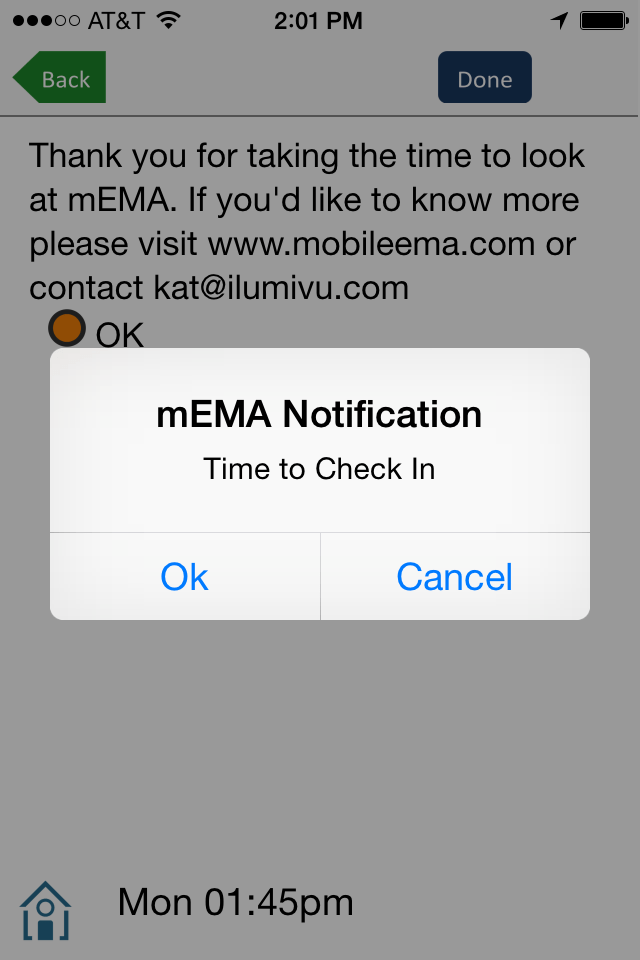
\includegraphics[width=0.3\linewidth]{images/instruments/ilumivu/iv-app-1} 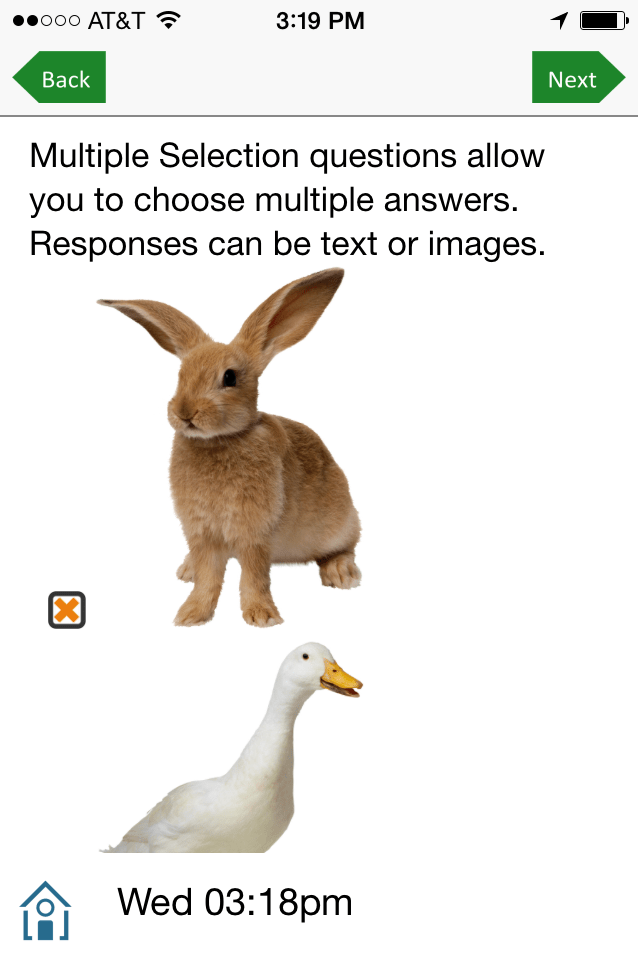
\includegraphics[width=0.3\linewidth]{images/instruments/ilumivu/iv-app-2} 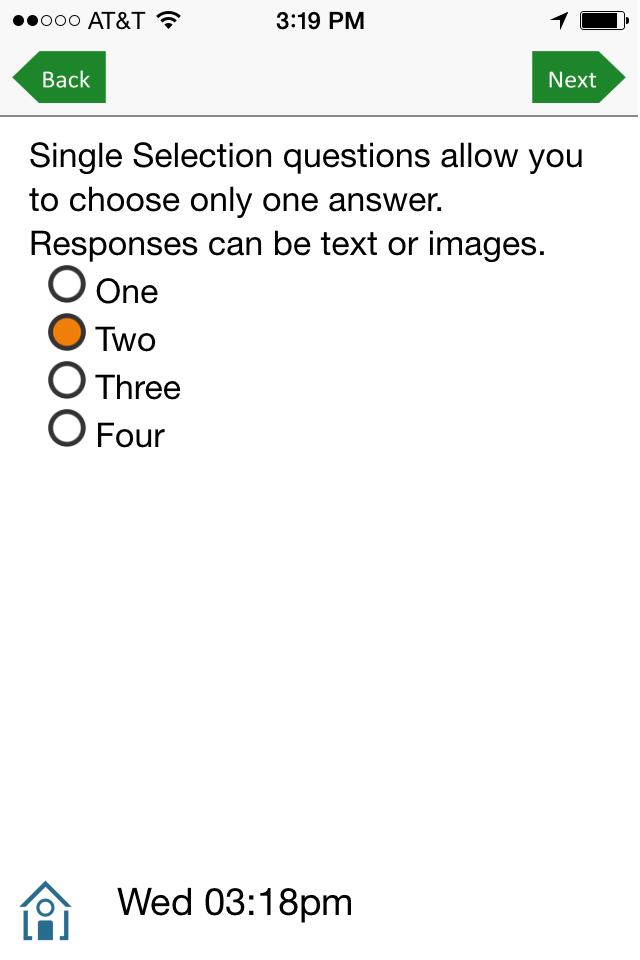
\includegraphics[width=0.3\linewidth]{images/instruments/ilumivu/iv-app-3} 

}

\caption{Ilumivu App Screenshots}\label{fig:ilumivu}
\end{figure}

\subsection{Moodbuster}\label{moodbuster}

\index{Moodbuster}

Moodbuster (\url{http://moodbuster.eu/}) is a web-based treatment
platform with an integrated EMA app. The platform was developed by an
international non-profit research consortium, including VU, VUmc and GGZ
inGeest, in two major EU-funded research projects: ICT4Depression
\citep[see ICT4Depression.eu;][]{warmerdam2012} and E-COMPARED
\citep[see \url{http://e-compared.eu};][]{Kleiboer2016, VandeVen2017}.

In the E-COMPARED trial, Moodbuster was used, in five EU-countries, to
test blended treatment of major depression. In this study, participants
used the smartphone app to rate mood and various other
depression-related variables, in the context of their treatment, over a
period of up to 20 weeks.

E-COMPARED EMA data were used in several predictive machine learning
studies \citep{mikus2018, rocha2018}. In addition, the EMA app was used
in a satellite study designed to assess the effects of long-term EMA
\citep{VanBallegooijen2016}. Moodbuster will also be used in the EU
ImpleMentAll project (\url{http://www.implementall.eu}) and in several
other clinical trials that are in preparation. Currently, EMA assessment
protocols are hard-coded in the Moodbuster app. New EMA assessments
protocols can be implemented in collaboration with the Moodbuster
development team. An online back-office is in development. Previous
studies used an Android version of the EMA app. Cross-platform versions
of the app are in development.

More information on Moodbuster can be obtained from prof. dr. Heleen
Riper (\href{mailto:h.riper@vu.nl}{\nolinkurl{h.riper@vu.nl}}).

\begin{figure}[!t]

{\centering 
\includegraphics[width=0.25\linewidth]{images/instruments/moodbuster/mb-app-home} 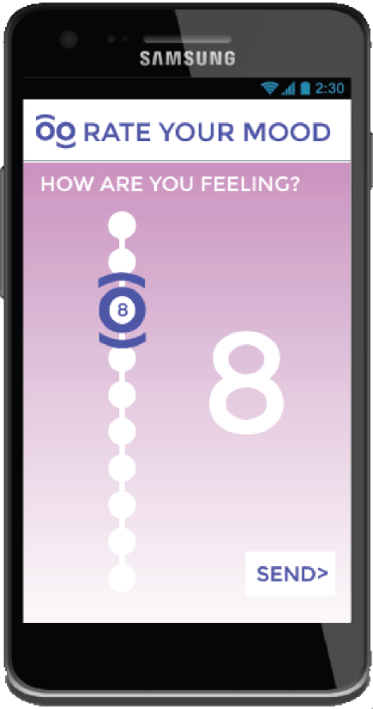
\includegraphics[width=0.25\linewidth]{images/instruments/moodbuster/mb-app-mood} 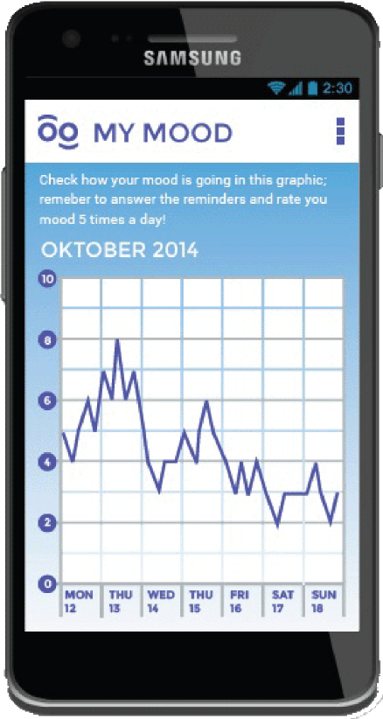
\includegraphics[width=0.25\linewidth]{images/instruments/moodbuster/mb-app-graph} 

}

\caption{MoodBuster App Screenshots}\label{fig:moodbuster}
\end{figure}

\subsection{Movisens}\label{movisens}

\index{Movisens}

Movisens (\url{http://www.movisens.com}) is a German company that is
specialized in the development of hard- and software solutions for
mobile sensing. The company sells small wearable devices that contain
several high-precision sensors, including an accelerometer, gyroscope,
barometer and thermometer. In addition, the company has developed an
(Android) app, called MovisensXS, which can be used for active EMA
research. The app can optionally be configured for smartphone logging
(e.g., to log music that a study participant listens this). The wearable
sensor can also be linked to the app, so that EMA questionnaires can be
triggered based on targeted activity or energy expenditure patterns,
such as extended periods of sedentary behavior.

Specialized software to import, pre-process and analyze raw sensor data
is available for download. Like Ilumivu, researchers can define EMA
sample schedules for their study in a web-based back-office
(\url{https://xs.movisens.com}), using an online graphical editor. Once
defined, participants can be invited to the study, through the
back-office, to download the freely available Movisens App from Google
Play store. The back-office also allows researchers to monitor study
compliance and download data.

MovisensXS EMA license costs vary from 500 to 10.000 euros per year,
depending on the required number of `credits' which are linked to the
number of EMA responses. Prospect users can test platform, without
functional restrictions, with a free test account. An EMA test-study can
thus be set up and started in less than a day. A current (November 2018)
limitation of Movisens is the lack of an iOS version of the EMA app.
Study participants who own an iPhone have to be excluded from studies,
or will have to be provided with an Android phone.

\begin{figure}[!t]

{\centering 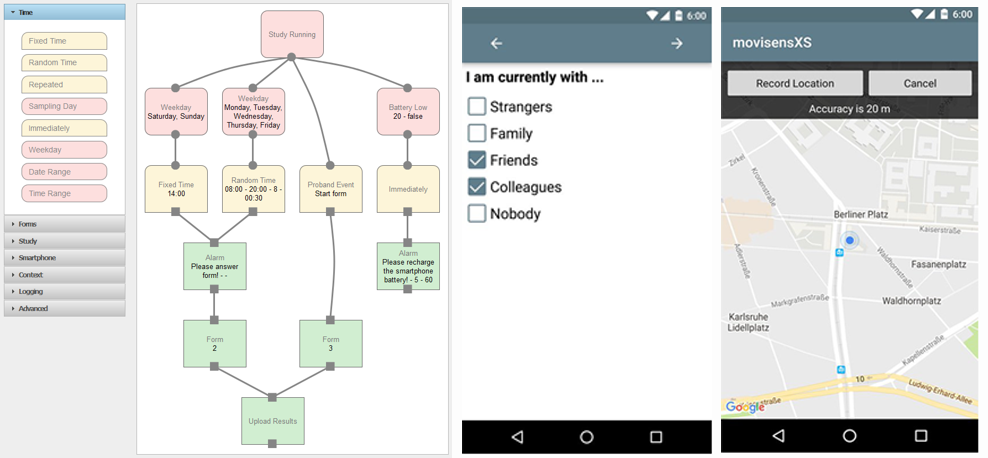
\includegraphics[width=0.8\linewidth]{images/instruments/movisens/movisens} 

}

\caption{Movisens Sample scheme editor (left) and App Screenshots (right)}\label{fig:movisens}
\end{figure}

\subsection{PsyMate}\label{psymate}

\index{PsyMate}

The PsyMate app (\url{http://www.psymate.eu}) was developed by the
Department of Psychiatry and Psychology at Maastricht University in the
Netherlands to assess psychological problems in daily life. The app has
been validated for use in depression, bipolar disorder, and psychosis,
with new scales currently being developed for a range of diseases
including Parkinson's disease, pain, cardiology, hypertension, diabetes
and Irritable Bowel Syndrome. It was also used in an EU-funded project
to study gene-environment interaction in schizophrenia
(\url{http://www.eu-gei.eu/about-the-project/psymate}).

The app is free to download for iOS and Android devices on Apple and
Google play stores. PsyMate is available in five languages (English,
French, German, Dutch, Spanish). More translations are in preparation.

Uses of the app include self-monitoring of mood states, delivering
professional support during treatment, or conducting EMA-research. The
app can be customized to address specific client needs or research
projects, with expertise from the PsyMate development team, which
includes an active working group that meets regularly to discuss and
advise new projects. Researchers have access to the raw data without
having to go through the PsyMate development team. Communication from
the PsyMate back office to researchers about updates and assistance with
technical problems could be a point for consideration for using this
platform.

\begin{figure}[!t]

{\centering 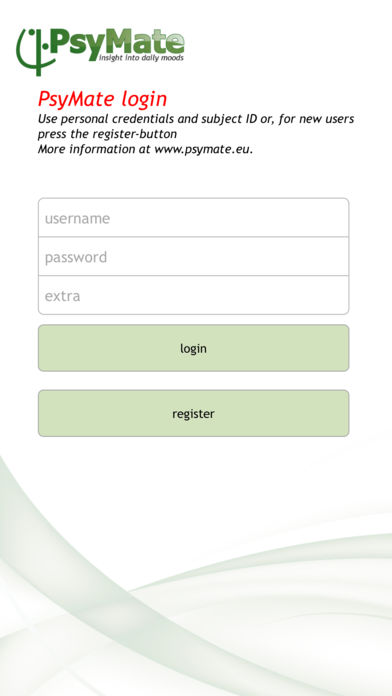
\includegraphics[width=0.25\linewidth]{images/instruments/psymate/psymate-app1} 
\includegraphics[width=0.25\linewidth]{images/instruments/psymate/psymate-app3} 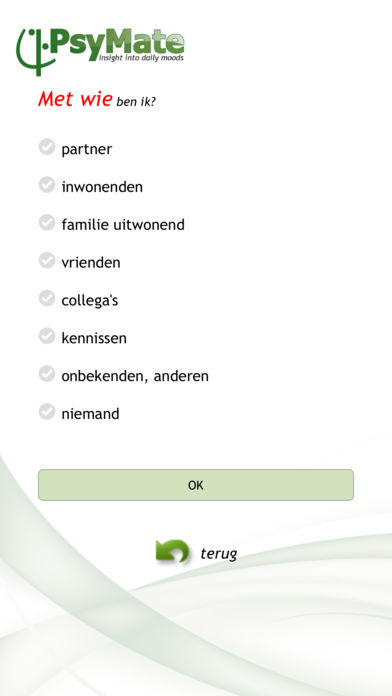
\includegraphics[width=0.25\linewidth]{images/instruments/psymate/psymate-app4} 

}

\caption{PsyMate App Screenshots}\label{fig:psymate}
\end{figure}

\subsection{RoQua}\label{roqua}

\index{RoQua}

RoQua (\url{http://www.roqua.nl/}) is a web-based Routine Outcome
Monitoring system, developed and maintained by a Dutch non-profit
development and service organization that is funded by several by
northern GGZ organizations and the Department of Psychiatry, University
Medical Center Groningen. RoQUA has a sophisticated and user-friendly
online back-office portal, with which researchers can define assessment
protocols and invite study participants - through e-mail or SMS - to
complete questionnaires online (on desktop or mobile devices).

By inviting study participants several times a day to complete a
questionnaire via the standard web browser of their mobile phone, active
EMA an be implemented. This approach was taken in several large-scale
studies, including `NESDA' \citep[\url{http://nesda.nl}; see also
Chapter \ref{catalogue}) and `HowNutsAreTheDutch'
(\url{http://www.hoegekis.nl};][]{VanDerKrieke2017, VanDerKrieke2016}.
At present, RoQua does not support the collection of passive EMA data.
However, preliminary results have been reported with a system called
`Physiqual' \citep{Blaauw2016}, with which active EMA data, collected
with RoQUA, can be combined with wearable sensor data.

\begin{figure}[!t]

{\centering 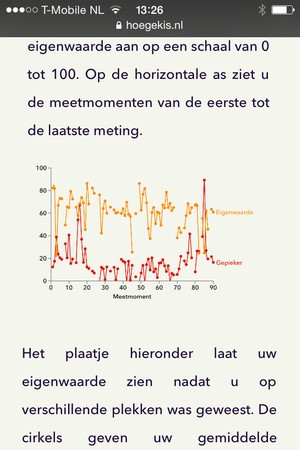
\includegraphics[width=0.25\linewidth]{images/instruments/roqua/roqua_p1} 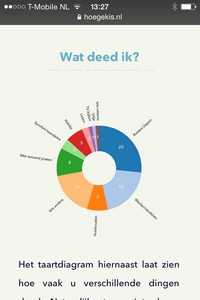
\includegraphics[width=0.25\linewidth]{images/instruments/roqua/roqua_p2} \includegraphics[width=0.25\linewidth]{images/instruments/roqua/roqua_p3} 

}

\caption{Screenshots of the participant feedback web-page of the 'HowNutsAreTheDutch' project, in which data is collected by the RoQua system}\label{fig:roqua}
\end{figure}

\section{Wearables}\label{wearables}

\subsection{GENEActiv}\label{geneactiv}

\index{GENEActiv} \index{Actant - Activity Analysis Toolbox}

GENEActiv, sold by UK-based company Activinsights
(\url{http://activinsights.com}), is a waterproof wrist-worn device with
a high-precision, configurable 3-axial accelerometer (range: +/- 8g), an
ambient light sensor, a (near-body) temperature sensor, and an event
logger (a button that users can press to mark a targeted event).
GENEActiv was developed to accurately assess human activity in
scientific studies. The device has a storage capacity of 0.5GB of raw
data. At 10Hz, the device can log activity up to one month. July 2018,
the price for one unit was approximately 250 euro.

GENEActiv is used in a growing number of clinical studies to measure
activity and sleep-wake cycles, in natural conditions, over longer
periods of time. Dedicated R-packages to pre-process and analyze the raw
data exist (see Chapter \ref{rcat}). Matlab users should consider the
open source `Actant - Activity Analysis Toolbox'
(\url{https://github.com/maximosipov/actant}), by Osipov \& Te Lindert,
which includes functionality for visualization and analysis of
behavioral and environmental timeseries, acquired using GENEActiv (and
other) accelerometers. No accompanying app exists with which study
participants can be provided feedback about their activity. This might
negatively affect wear-time and study compliance in research
participants, who are accustomed to consumer activity-sampling devices,
such as Fitbit, where many options for real-time feedback exist.
Further, researchers we spoke with noted that the event logger was hard
to use in practice. This resulted in low compliance in field studies.

\begin{figure}[!h]

{\centering \includegraphics[width=1\linewidth]{images/instruments/geneactive/geneactive-pack} 

}

\caption{The GENEActiv Accelerometer}\label{fig:geneactiv}
\end{figure}

\subsection{VU-AMS}\label{vu-ams}

\index{VU-AMS} \index{DAMS}
\index{Autonomic and cardiovascular activity}

The VU University Ambulatory Monitoring System (VU-AMS;
\url{http://www.vu-ams.nl/}), developed by the department of Biological
Psychology and the Technical Department (ITM) of the Faculty of
Behavioral and Movement Sciences, allows ambulatory recording of
autonomic and cardiovascular activity. VU-AMS measures heart rate, heart
rate variability, Respiratory Sinus Arrhythmia, Pre-Ejection Period,
Left Ventricular Ejection Time, Respiration Rate, Stroke Volume (SV) and
Cardiac Output, Skin Conductance Level (SCL) and Skin Conductance
Responses (SCRs) and Tri-Axial Accelerometry (of Body Movement). For the
processing of VU-AMS data, a dedicated software suite called the `Data
Analysis and Management Software' (VU-DAMS) is available (for Windows
and Mac). VU-AMS is used worldwide by many research groups, to study
stress and emotion in both laboratory and naturalistic settings
\citep{DeGeus1995, Geus1996, Willemsen1996}.

\begin{figure}[!t]

{\centering \includegraphics[width=1\linewidth]{images/instruments/VU-AMS/VU_AMS2} 

}

\caption{VU-AMS device (left) and VU-DAMS screenshot (right)}\label{fig:vu-ams}
\end{figure}

\chapter{R Packages for EMA Research}\label{rcat}

Many R packages exist that can help you in the management and analysis
of EMA data. In this chapter, a selection of these packages is
discussed. For each, we provide a summary description, example code, and
pointers to further documentation, to give you a head start in using
these packages for your work.

\begin{longtable}[]{@{}lll@{}}
\caption{\label{tab:rcat} List of R packages that are useful in EMA
research.}\tabularnewline
\toprule
\begin{minipage}[b]{0.21\columnwidth}\raggedright\strut
\textbf{Category}\strut
\end{minipage} & \begin{minipage}[b]{0.23\columnwidth}\raggedright\strut
\textbf{Package}\strut
\end{minipage} & \begin{minipage}[b]{0.48\columnwidth}\raggedright\strut
\textbf{Description}\strut
\end{minipage}\tabularnewline
\midrule
\endfirsthead
\toprule
\begin{minipage}[b]{0.21\columnwidth}\raggedright\strut
\textbf{Category}\strut
\end{minipage} & \begin{minipage}[b]{0.23\columnwidth}\raggedright\strut
\textbf{Package}\strut
\end{minipage} & \begin{minipage}[b]{0.48\columnwidth}\raggedright\strut
\textbf{Description}\strut
\end{minipage}\tabularnewline
\midrule
\endhead
\begin{minipage}[t]{0.21\columnwidth}\raggedright\strut
\textbf{Actigraphy}\strut
\end{minipage} & \begin{minipage}[t]{0.23\columnwidth}\raggedright\strut
GENEAread / GGIR\strut
\end{minipage} & \begin{minipage}[t]{0.48\columnwidth}\raggedright\strut
Import, pre-process and analyze raw accelerometer data.\strut
\end{minipage}\tabularnewline
\begin{minipage}[t]{0.21\columnwidth}\raggedright\strut
\strut
\end{minipage} & \begin{minipage}[t]{0.23\columnwidth}\raggedright\strut
PhysicalActivity\strut
\end{minipage} & \begin{minipage}[t]{0.48\columnwidth}\raggedright\strut
Analyze Actigraph accelerometer data.\strut
\end{minipage}\tabularnewline
\begin{minipage}[t]{0.21\columnwidth}\raggedright\strut
\textbf{Data Management \& Visual Exploration}\strut
\end{minipage} & \begin{minipage}[t]{0.23\columnwidth}\raggedright\strut
dplyr\strut
\end{minipage} & \begin{minipage}[t]{0.48\columnwidth}\raggedright\strut
Data transformation.\strut
\end{minipage}\tabularnewline
\begin{minipage}[t]{0.21\columnwidth}\raggedright\strut
\strut
\end{minipage} & \begin{minipage}[t]{0.23\columnwidth}\raggedright\strut
ggplot2\strut
\end{minipage} & \begin{minipage}[t]{0.48\columnwidth}\raggedright\strut
Create graphs.\strut
\end{minipage}\tabularnewline
\begin{minipage}[t]{0.21\columnwidth}\raggedright\strut
\strut
\end{minipage} & \begin{minipage}[t]{0.23\columnwidth}\raggedright\strut
haven\strut
\end{minipage} & \begin{minipage}[t]{0.48\columnwidth}\raggedright\strut
Import and export SPSS data files.\strut
\end{minipage}\tabularnewline
\begin{minipage}[t]{0.21\columnwidth}\raggedright\strut
\strut
\end{minipage} & \begin{minipage}[t]{0.23\columnwidth}\raggedright\strut
lubridate\strut
\end{minipage} & \begin{minipage}[t]{0.48\columnwidth}\raggedright\strut
Manipulate date and time variables.\strut
\end{minipage}\tabularnewline
\begin{minipage}[t]{0.21\columnwidth}\raggedright\strut
\textbf{Auto-regressive modeling}\strut
\end{minipage} & \begin{minipage}[t]{0.23\columnwidth}\raggedright\strut
autovarCore\strut
\end{minipage} & \begin{minipage}[t]{0.48\columnwidth}\raggedright\strut
Automate the construction of vector autoregressive models.\strut
\end{minipage}\tabularnewline
\begin{minipage}[t]{0.21\columnwidth}\raggedright\strut
\textbf{Mixed-effects Modeling}\strut
\end{minipage} & \begin{minipage}[t]{0.23\columnwidth}\raggedright\strut
lme4\strut
\end{minipage} & \begin{minipage}[t]{0.48\columnwidth}\raggedright\strut
Fit linear and nonlinear mixed-effects models. Fast alternative to
package \texttt{nlme}.\strut
\end{minipage}\tabularnewline
\begin{minipage}[t]{0.21\columnwidth}\raggedright\strut
\strut
\end{minipage} & \begin{minipage}[t]{0.23\columnwidth}\raggedright\strut
nlme\strut
\end{minipage} & \begin{minipage}[t]{0.48\columnwidth}\raggedright\strut
Fit linear and nonlinear mixed effects models. Pre-dates package
\texttt{lme4}, but is still used because it a provides advanced options
to model correlational structures\strut
\end{minipage}\tabularnewline
\begin{minipage}[t]{0.21\columnwidth}\raggedright\strut
\textbf{Simulation}\strut
\end{minipage} & \begin{minipage}[t]{0.23\columnwidth}\raggedright\strut
simr\strut
\end{minipage} & \begin{minipage}[t]{0.48\columnwidth}\raggedright\strut
Simulation-based power calculations for mixed models.\strut
\end{minipage}\tabularnewline
\begin{minipage}[t]{0.21\columnwidth}\raggedright\strut
\strut
\end{minipage} & \begin{minipage}[t]{0.23\columnwidth}\raggedright\strut
simstudy\strut
\end{minipage} & \begin{minipage}[t]{0.48\columnwidth}\raggedright\strut
Simulate complex study data.\strut
\end{minipage}\tabularnewline
\begin{minipage}[t]{0.21\columnwidth}\raggedright\strut
\textbf{Symptom Networks}\strut
\end{minipage} & \begin{minipage}[t]{0.23\columnwidth}\raggedright\strut
bootnet\strut
\end{minipage} & \begin{minipage}[t]{0.48\columnwidth}\raggedright\strut
Assess the stability of symptom networks.\strut
\end{minipage}\tabularnewline
\begin{minipage}[t]{0.21\columnwidth}\raggedright\strut
\strut
\end{minipage} & \begin{minipage}[t]{0.23\columnwidth}\raggedright\strut
qgraph\strut
\end{minipage} & \begin{minipage}[t]{0.48\columnwidth}\raggedright\strut
Estimate and plot symptom networks.\strut
\end{minipage}\tabularnewline
\begin{minipage}[t]{0.21\columnwidth}\raggedright\strut
\textbf{Time series analysis}\strut
\end{minipage} & \begin{minipage}[t]{0.23\columnwidth}\raggedright\strut
lomb\strut
\end{minipage} & \begin{minipage}[t]{0.48\columnwidth}\raggedright\strut
Calculate the Lomb-Scargle Periodogram for unevenly sampled time
series.\strut
\end{minipage}\tabularnewline
\bottomrule
\end{longtable}

\textless{}\textless{}\textless{}\textless{}\textless{}\textless{}\textless{}
HEAD \#\# Actigraphy \index{Actigraphy}

Accelerometer data need considerable pre-processing before final
analyses can be run. Raw data have to be read in from a variety of
brand-specific file formats, data have to re-calibrated on a per-device
basis, non-wear periods have to detected, and summarizing measures, such
as activity counts and energy-expenditure measures, have to be
calculated from imputed triangular (x, y, x) data, often in several time
windows (i.e., epochs).

\subsection{GENEAread}\label{genearead}

\index{GENEAread}

\href{https://www.geneactiv.org/}{GENEActiv} is a wrist-worn
accelerometer that is widely used in sleep and physical activity
research. With package \textbf{GENEAread} \citep{R_GENEAread}, raw
GENEActiv binary files can be imported into R for further processing, as
illustrated below.

\begin{Shaded}
\begin{Highlighting}[]
\CommentTok{# Read raw GENEActiv data.}
\KeywordTok{library}\NormalTok{(GENEAread)}
\NormalTok{dat <-}\StringTok{ }\KeywordTok{read.bin}\NormalTok{(}\KeywordTok{system.file}\NormalTok{(}\StringTok{"binfile/TESTfile.bin"}\NormalTok{, }\DataTypeTok{package =} \StringTok{"GENEAread"}\NormalTok{),}
                  \DataTypeTok{verbose =} \OtherTok{FALSE}\NormalTok{, }\DataTypeTok{downsample =} \DecValTok{20}\NormalTok{)}
\NormalTok{d <-}\StringTok{ }\KeywordTok{as.data.frame}\NormalTok{(dat}\OperatorTok{$}\NormalTok{data.out)}
\NormalTok{d}\OperatorTok{$}\NormalTok{timestamp <-}\StringTok{ }\KeywordTok{as.POSIXct}\NormalTok{(d}\OperatorTok{$}\NormalTok{timestamp, }\DataTypeTok{origin =} \StringTok{"1970-01-01"}\NormalTok{, }\DataTypeTok{tz =} \StringTok{"UTC"}\NormalTok{)}
\NormalTok{d[}\DecValTok{1}\OperatorTok{:}\DecValTok{4}\NormalTok{, ]}
\end{Highlighting}
\end{Shaded}

\begin{tabular}{l|r|r|r|r|r|r}
\hline
timestamp & x & y & z & light & button & temperature\\
\hline
2012-05-23 16:47:50.0 & 0.023516 & -0.887283 & -0.100785 & 0 & 0 & 25.8\\
\hline
2012-05-23 16:47:50.2 & 0.027462 & -0.933668 & -0.140047 & 0 & 0 & 25.8\\
\hline
2012-05-23 16:47:50.4 & 0.035354 & -1.150135 & -0.030114 & 0 & 0 & 25.8\\
\hline
2012-05-23 16:47:50.5 & 0.070865 & -3.229764 & -0.619042 & 0 & 0 & 25.8\\
\hline
\end{tabular}

By having access to the raw data, you are free to explore the data
further in any you want. For instance, to plot the raw data captured by
each sensor, type:

\begin{Shaded}
\begin{Highlighting}[]
\CommentTok{# Plot raw GENEActive data, with ggplot}
\KeywordTok{library}\NormalTok{(ggplot2); }\KeywordTok{library}\NormalTok{(tidyr)}
\NormalTok{d <-}\StringTok{ }\KeywordTok{gather}\NormalTok{(d, }\DataTypeTok{key =} \StringTok{"sensor"}\NormalTok{, }\DataTypeTok{value =} \StringTok{"value"}\NormalTok{, }\OperatorTok{-}\NormalTok{timestamp)}
\KeywordTok{ggplot}\NormalTok{(d, }\KeywordTok{aes}\NormalTok{(}\DataTypeTok{x =}\NormalTok{ timestamp, }\DataTypeTok{y =}\NormalTok{ value)) }\OperatorTok{+}\StringTok{ }
\StringTok{  }\KeywordTok{geom_line}\NormalTok{() }\OperatorTok{+}\StringTok{ }
\StringTok{  }\KeywordTok{facet_wrap}\NormalTok{(}\OperatorTok{~}\NormalTok{sensor, }\DataTypeTok{scales =} \StringTok{"free_y"}\NormalTok{)}
\end{Highlighting}
\end{Shaded}

\begin{figure}

{\centering \includegraphics[width=1\linewidth]{R-package-catalogue_files/figure-latex/genearead-plot-example-1} 

}

\caption{Raw sensor data of a GENEActiv accelerometer.}\label{fig:genearead-plot-example}
\end{figure}

\subsection{GGIR}\label{ggir}

\index{GGIR}

Package \emph{GGIR} \citep{R-GGIR} is a package to pre-process raw
accelerometry data from three accelerometer brands:
\href{http://actigraphcorp.com/}{ActiGraph},
\href{http://axivity.com/}{Axivity}, and
\href{https://www.geneactiv.org/}{GENEActiv} (GGIR includes package
\texttt{GENEAread}). The package is in active development. New features
are introduced and bugs are fixed on a regular basis. If you consider to
use \texttt{GGIR} for your project, you may want to install the
development version, which is on
\href{https://github.com/wadpac/GGIR}{GitHub}.

\begin{Shaded}
\begin{Highlighting}[]
\KeywordTok{library}\NormalTok{(devtools)}
\KeywordTok{install_github}\NormalTok{(}\StringTok{"wadpac/GGIR"}\NormalTok{, }\DataTypeTok{dependencies =} \OtherTok{TRUE}\NormalTok{)}
\end{Highlighting}
\end{Shaded}

\texttt{GGIR}'s main function is \texttt{g.shell.GGIR}, with which
multiple accelerometer data files can be imported, calibrated, cleaned
and analyzed. The example below shows an example configuration of this
function. See \texttt{?g.shell.GGIR} (and \texttt{?g.part1},
?\texttt{g.part2}, to \texttt{g.part5}) to learn the meaning of each
parameter. If you get lost or run into a problem, you can ask the
package developers or other users for help via the GGIR Google
discussion forum, at
\url{https://groups.google.com/forum/\#!forum/rpackageggir}.

\begin{Shaded}
\begin{Highlighting}[]
\CommentTok{# Import actigraphy data with GGIR}
\KeywordTok{library}\NormalTok{(GGIR)}
\KeywordTok{g.shell.GGIR}\NormalTok{(}\CommentTok{#=======================================}
             \CommentTok{# Shell configuration:}
             \DataTypeTok{mode =} \KeywordTok{c}\NormalTok{(}\DecValTok{1}\NormalTok{, }\DecValTok{2}\NormalTok{, }\DecValTok{3}\NormalTok{, }\DecValTok{4}\NormalTok{),}
             \DataTypeTok{datadir=}\StringTok{"./data/raw"}\NormalTok{, }\DataTypeTok{outputdir=}\StringTok{"./data"}\NormalTok{,}
             \DataTypeTok{desiredtz =} \StringTok{"Europe/Amsterdam"}\NormalTok{, }\CommentTok{# set timezone!}
             \DataTypeTok{f0 =} \DecValTok{1}\NormalTok{, }\DataTypeTok{f1 =} \DecValTok{2}\NormalTok{, }\DataTypeTok{overwrite =} \OtherTok{FALSE}\NormalTok{,}
             \CommentTok{#-------------------------------}
             \CommentTok{# Part 1: read, calibrate, extract features}
             \DataTypeTok{do.enmo =} \OtherTok{TRUE}\NormalTok{, }\DataTypeTok{do.anglez=}\OtherTok{TRUE}\NormalTok{,}
             \DataTypeTok{chunksize =} \DecValTok{1}\NormalTok{, }\DataTypeTok{printsummary =} \OtherTok{TRUE}\NormalTok{,}
             \CommentTok{#-------------------------------}
             \CommentTok{# Part 2:}
             \DataTypeTok{strategy =} \DecValTok{1}\NormalTok{, }\DataTypeTok{ndayswindow=}\DecValTok{7}\NormalTok{,}
             \DataTypeTok{hrs.del.start =} \DecValTok{0}\NormalTok{, }\DataTypeTok{hrs.del.end =} \DecValTok{0}\NormalTok{,}
             \DataTypeTok{maxdur =} \DecValTok{8}\NormalTok{,  }\DataTypeTok{includedaycrit =} \DecValTok{10}\NormalTok{,}
             \DataTypeTok{winhr =} \KeywordTok{c}\NormalTok{(}\DecValTok{5}\NormalTok{,}\DecValTok{10}\NormalTok{),}
             \DataTypeTok{qlevels =} \KeywordTok{c}\NormalTok{(}\KeywordTok{c}\NormalTok{(}\DecValTok{1380}\OperatorTok{/}\DecValTok{1440}\NormalTok{),}\KeywordTok{c}\NormalTok{(}\DecValTok{1410}\OperatorTok{/}\DecValTok{1440}\NormalTok{)),}
             \DataTypeTok{qwindow =} \KeywordTok{c}\NormalTok{(}\DecValTok{0}\NormalTok{,}\DecValTok{24}\NormalTok{),}
             \DataTypeTok{ilevels =} \KeywordTok{c}\NormalTok{(}\KeywordTok{seq}\NormalTok{(}\DecValTok{0}\NormalTok{, }\DecValTok{400}\NormalTok{, }\DataTypeTok{by=}\DecValTok{50}\NormalTok{), }\DecValTok{8000}\NormalTok{),}
             \DataTypeTok{mvpathreshold =} \KeywordTok{c}\NormalTok{(}\DecValTok{100}\NormalTok{,}\DecValTok{125}\NormalTok{), }
             \DataTypeTok{bout.metric =} \DecValTok{4}\NormalTok{, }\DataTypeTok{closedbout =} \OtherTok{FALSE}\NormalTok{,}
             \CommentTok{#-------------------------------}
             \CommentTok{# Part 3: Sleep detection}
             \CommentTok{#-------------------------------}
             \DataTypeTok{timethreshold=} \KeywordTok{c}\NormalTok{(}\DecValTok{5}\NormalTok{), }\DataTypeTok{anglethreshold=}\DecValTok{5}\NormalTok{,}
             \DataTypeTok{ignorenonwear =} \OtherTok{TRUE}\NormalTok{,}
             \CommentTok{#-------------------------------}
             \CommentTok{# Part 4: Sleep summaries (per person)}
             \DataTypeTok{excludefirstlast =} \OtherTok{TRUE}\NormalTok{, }\DataTypeTok{includenightcrit =} \DecValTok{16}\NormalTok{,}
             \DataTypeTok{def.noc.sleep =} \KeywordTok{c}\NormalTok{(}\DecValTok{21}\NormalTok{, }\DecValTok{9}\NormalTok{),}
             \DataTypeTok{relyonsleeplog =} \OtherTok{TRUE}\NormalTok{, }\DataTypeTok{nnights =} \DecValTok{3}\NormalTok{,}
             \CommentTok{#-----------------------------------}
             \CommentTok{# Report generation}
             \DataTypeTok{do.report =} \KeywordTok{c}\NormalTok{(}\DecValTok{2}\NormalTok{, }\DecValTok{4}\NormalTok{), }\DataTypeTok{visualreport =} \OtherTok{TRUE}\NormalTok{,}
             \DataTypeTok{dofirstpage =} \OtherTok{TRUE}\NormalTok{, }\DataTypeTok{viewingwindow =} \DecValTok{1}
\NormalTok{)}
\end{Highlighting}
\end{Shaded}

\subsection{PhysicalActivity}\label{physicalactivity}

\index{PhysicalActivity}

Package \emph{PhysicalActivity} \citep{R-PhysicalActivity} provides an
alternative to packages \texttt{GGIR} and \texttt{GENEAread}, when
\href{https://actigraphcorp.com/}{ActiGraph} data are available.

\begin{Shaded}
\begin{Highlighting}[]
\CommentTok{# Plotting activity counts.}
\KeywordTok{library}\NormalTok{(PhysicalActivity)}
\KeywordTok{library}\NormalTok{(ggplot2)}

\KeywordTok{data}\NormalTok{(dataSec)}

\NormalTok{d <-}\StringTok{ }\KeywordTok{dataCollapser}\NormalTok{(dataSec, }\DataTypeTok{TS =} \StringTok{"TimeStamp"}\NormalTok{, }\DataTypeTok{col =} \StringTok{"counts"}\NormalTok{, }\DataTypeTok{by =} \DecValTok{300}\NormalTok{)}

\KeywordTok{ggplot}\NormalTok{(d, }\KeywordTok{aes}\NormalTok{(}\DataTypeTok{x =} \KeywordTok{as.POSIXct}\NormalTok{(TimeStamp), }\DataTypeTok{y =}\NormalTok{ counts)) }\OperatorTok{+}
\StringTok{  }\KeywordTok{geom_line}\NormalTok{(}\DataTypeTok{size =}\NormalTok{ .}\DecValTok{5}\NormalTok{, }\DataTypeTok{alpha =}\NormalTok{ .}\DecValTok{5}\NormalTok{) }\OperatorTok{+}
\StringTok{  }\KeywordTok{xlab}\NormalTok{(}\StringTok{"Time"}\NormalTok{) }\OperatorTok{+}\StringTok{ }\KeywordTok{ylab}\NormalTok{(}\StringTok{"Activity Counts"}\NormalTok{)}
\end{Highlighting}
\end{Shaded}

\begin{figure}

{\centering \includegraphics[width=1\linewidth]{R-package-catalogue_files/figure-latex/fig15a-1} 

}

\caption{Activity Counts (5-minute windows), in a Three-day Accelerometer data set.}\label{fig:fig15a}
\end{figure}

\section{Autoregressive modeling}\label{autoregressive-modeling}

\subsection{autovarCore}\label{autovarcore}

\index{autovarCore} \index{autovar}

\index{Vector autoregressive models}

Vector autoregressive (VAR) models can be used to detect lagged
relationships between multiple time-series (see also Chapter
\ref{features}). In VAR, each variable is modeled as a linear function
of past values (lags) of itself and of present and past values of other
variables. When EMA is used to capture multiple phenomena over time, VAR
can provide insight in how these phenomena interact. One challenge in
VAR modelling is that many alternative models potentially exist, Package
\emph{autovarCore} \citep{R-autovarCore} was developed to help
researchers to find the VAR model with the best fit to a given
time-series data set. In the example below, function \texttt{autovar} is
used to detect that changes in depression are positively related to past
(lag 1) values of activity, in a simulated data set:

\begin{Shaded}
\begin{Highlighting}[]
\CommentTok{# Autovar analysis.}
\KeywordTok{library}\NormalTok{(autovarCore)}

\CommentTok{# simulate data}
\NormalTok{N =}\StringTok{ }\DecValTok{100}
\NormalTok{depression <-}\StringTok{ }\KeywordTok{rnorm}\NormalTok{(N)}
\NormalTok{activity <-}\StringTok{ }\KeywordTok{rnorm}\NormalTok{(N)}
\NormalTok{activity_lag1 <-}\StringTok{ }\KeywordTok{c}\NormalTok{(}\OtherTok{NA}\NormalTok{, activity[}\DecValTok{1}\OperatorTok{:}\NormalTok{(N }\OperatorTok{-}\DecValTok{1}\NormalTok{)])}

\NormalTok{depression <-}\StringTok{ }\NormalTok{depression }\OperatorTok{+}\StringTok{ }\FloatTok{0.5} \OperatorTok{*}\StringTok{ }\NormalTok{activity_lag1 }
\NormalTok{d <-}\StringTok{ }\KeywordTok{data.frame}\NormalTok{(depression, activity)}

\NormalTok{models_found <-}\StringTok{ }\NormalTok{autovarCore}\OperatorTok{::}\KeywordTok{autovar}\NormalTok{(d, }\DataTypeTok{selected_column_names =} \KeywordTok{c}\NormalTok{(}\StringTok{'activity'}\NormalTok{, }\StringTok{'depression'}\NormalTok{))}

\CommentTok{# Show details for the best model found}
\KeywordTok{summary}\NormalTok{(models_found[[}\DecValTok{1}\NormalTok{]]}\OperatorTok{$}\NormalTok{varest}\OperatorTok{$}\NormalTok{varresult}\OperatorTok{$}\NormalTok{depression)}
\CommentTok{#> }
\CommentTok{#> Call:}
\CommentTok{#> lm(formula = y ~ -1 + ., data = datares)}
\CommentTok{#> }
\CommentTok{#> Residuals:}
\CommentTok{#>     Min      1Q  Median      3Q     Max }
\CommentTok{#> -2.3230 -0.6354  0.1325  0.6432  1.9003 }
\CommentTok{#> }
\CommentTok{#> Coefficients:}
\CommentTok{#>               Estimate Std. Error t value Pr(>|t|)    }
\CommentTok{#> activity.l1    0.45171    0.08130   5.556 2.56e-07 ***}
\CommentTok{#> depression.l1  0.12774    0.08780   1.455    0.149    }
\CommentTok{#> depression.l2 -0.10841    0.08780  -1.235    0.220    }
\CommentTok{#> const         -0.13312    0.09584  -1.389    0.168    }
\CommentTok{#> ---}
\CommentTok{#> Signif. codes:  0 '***' 0.001 '**' 0.01 '*' 0.05 '.' 0.1 ' ' 1}
\CommentTok{#> }
\CommentTok{#> Residual standard error: 0.937 on 94 degrees of freedom}
\CommentTok{#> Multiple R-squared:  0.2578, Adjusted R-squared:  0.2342 }
\CommentTok{#> F-statistic: 10.89 on 3 and 94 DF,  p-value: 3.337e-06}
\end{Highlighting}
\end{Shaded}

\texttt{AutovarCore} is a simplified version of a more extensive package
\emph{autovar} \citep{R-autovarCore}, which was used in several
publications \citep{VanderKrieke2015, Emerencia2016}. Further
information can be found on
\href{https://autovar.nl/}{http://autovar.nl} and
\href{https://autovarcore.nl/}{http://autovarcore.nl}

\section{Data management \& Visual
Exploration}\label{data-management-visual-exploration}

\index{tidyverse}

The \emph{tidyverse} is a collection of well-designed packages, authored
by the team behind RStudio, that together add a consistent, modern, and
efficient extension of base R functions. The \texttt{tidyverse} includes
popular packages such as \texttt{ggplot2} (for plotting), \texttt{haven}
(to read SPSS files), \texttt{dplyr} (for data manipulation), and many
more (see: \url{http://tidyverse.org} for a full list).

\subsection{dplyr}\label{dplyr}

\index{dplyr}

Package \emph{dplyr} \citep{R-dplyr} implements the
`split-apply-combine'-strategy. With \texttt{dplyr}, elementary data
manipulations can be e chained (using the pipe operator
\texttt{\%\textbackslash{}\textgreater{}\%}) to elegantly implement
complex data transformations.

\begin{Shaded}
\begin{Highlighting}[]
\CommentTok{# Aggregate data by ID, through a 'pipe'.}
\KeywordTok{require}\NormalTok{(dplyr)}

\NormalTok{d <-}\StringTok{ }\KeywordTok{data.frame}\NormalTok{(}
  \DataTypeTok{id =} \KeywordTok{factor}\NormalTok{(}\KeywordTok{rep}\NormalTok{(}\DecValTok{1}\OperatorTok{:}\DecValTok{5}\NormalTok{, }\DataTypeTok{each =} \DecValTok{10}\NormalTok{)), }
  \DataTypeTok{score =} \KeywordTok{rnorm}\NormalTok{(}\DecValTok{50}\NormalTok{)}
\NormalTok{)}

\NormalTok{b <-}\StringTok{ }\KeywordTok{as_tibble}\NormalTok{(d) }\OperatorTok\StringTok{ }
\StringTok{  }\KeywordTok{group_by}\NormalTok{(id) }\OperatorTok
\StringTok{  }\KeywordTok{summarize}\NormalTok{(}\DataTypeTok{mean =} \KeywordTok{mean}\NormalTok{(score))}

\NormalTok{knitr}\OperatorTok{::}\KeywordTok{kable}\NormalTok{(b)}
\end{Highlighting}
\end{Shaded}

\begin{tabular}{l|r}
\hline
id & mean\\
\hline
1 & 0.4859577\\
\hline
2 & 0.1336322\\
\hline
3 & -0.2648633\\
\hline
4 & 0.3439284\\
\hline
5 & -0.0146370\\
\hline
\end{tabular}

A good introduction to \texttt{dplyr} can be found in the book `R for
Data Science' \citep{wickham2016r}, which can be freely accessed online
(\url{http://r4ds.had.co.nz/}).

\subsection{ggplot2}\label{ggplot2}

\index{ggplot2}

Package \emph{ggplot2} \citep{wickham2016ggplot2} provides a collection
of high-level plotting commands with which graphs can be build up in
layers. It is based on `The Grammar of Graphics' \citep{wilkinson2006},
an influential analysis of the structure of scientific graphs.
Systematic introductions are available on the
\href{http://ggplot2.tidyverse.org/}{the tidyverse website}, and in the
book `ggplot2: Elegant Graphics for Data Analysis'
\citep{wickham2016ggplot2}.

The example below illustrates how graphs are layered. In the first step,
a coordinate system is set up. In step 2, all time/scores points are
plotted. In step 3, a smoothed line is fitted through these points.
Finally, in step 4, the graph is split on a variable ID (a subject
identifier), to show individual trajectories.

\begin{Shaded}
\begin{Highlighting}[]
\CommentTok{# Simple ggplot example.}
\KeywordTok{library}\NormalTok{(ggplot2)}

\CommentTok{# simulate example data }
\NormalTok{d =}\StringTok{ }\KeywordTok{data.frame}\NormalTok{(}
  \DataTypeTok{ID    =} \KeywordTok{rep}\NormalTok{(}\DecValTok{1}\OperatorTok{:}\DecValTok{4}\NormalTok{, }\DataTypeTok{each =} \DecValTok{25}\NormalTok{),}
  \DataTypeTok{time  =} \KeywordTok{rep}\NormalTok{(}\DecValTok{1}\OperatorTok{:}\DecValTok{25}\NormalTok{, }\DecValTok{4}\NormalTok{), }
  \DataTypeTok{score =} \KeywordTok{rnorm}\NormalTok{(}\DecValTok{100}\NormalTok{, }\DecValTok{0}\NormalTok{, }\DecValTok{2}\NormalTok{))}

\CommentTok{# step 1: initialise the coordinate system}
\NormalTok{g <-}\StringTok{ }\KeywordTok{ggplot}\NormalTok{(d, }\KeywordTok{aes}\NormalTok{(}\DataTypeTok{x =}\NormalTok{ time, }\DataTypeTok{y =}\NormalTok{ score)); g}

\CommentTok{# step 2: add scatterplot}
\NormalTok{g <-}\StringTok{ }\NormalTok{g }\OperatorTok{+}\StringTok{ }\KeywordTok{geom_point}\NormalTok{(); g}

\CommentTok{# step 3: add a smoothed line}
\NormalTok{g <-}\StringTok{ }\NormalTok{g }\OperatorTok{+}\StringTok{ }\KeywordTok{geom_smooth}\NormalTok{(}\DataTypeTok{method =} \StringTok{"loess"}\NormalTok{); g}

\CommentTok{# step 4: split plot by subject ID}
\NormalTok{g }\OperatorTok{+}\StringTok{ }\KeywordTok{facet_wrap}\NormalTok{(}\OperatorTok{~}\StringTok{ }\NormalTok{ID)}
\end{Highlighting}
\end{Shaded}

\begin{figure}

{\centering \includegraphics[width=0.45\linewidth]{R-package-catalogue_files/figure-latex/ggplot2-example-1} \includegraphics[width=0.45\linewidth]{R-package-catalogue_files/figure-latex/ggplot2-example-2} \includegraphics[width=0.45\linewidth]{R-package-catalogue_files/figure-latex/ggplot2-example-3} \includegraphics[width=0.45\linewidth]{R-package-catalogue_files/figure-latex/ggplot2-example-4} 

}

\caption{Plotting layers with ggplot2}\label{fig:ggplot2-example}
\end{figure}

\subsection{haven}\label{haven}

\index{haven} \index{SPSS}

With package \emph{haven} \citep{R-haven}, SPSS, STATA and SAS files can
be read into R. A particular advantage of the \texttt{read.sav} function
is that SPSS variables definitions are retained (in attributes of the
columns in the R \texttt{data.frames}).

\begin{Shaded}
\begin{Highlighting}[]
\CommentTok{# Read SPSS data}
\KeywordTok{library}\NormalTok{(haven)}

\CommentTok{# read example data (included in package)}
\NormalTok{path <-}\StringTok{ }\KeywordTok{system.file}\NormalTok{(}\StringTok{"examples"}\NormalTok{, }\StringTok{"iris.sav"}\NormalTok{, }\DataTypeTok{package =} \StringTok{"haven"}\NormalTok{)}
\NormalTok{d <-}\StringTok{ }\KeywordTok{read_sav}\NormalTok{(path)}

\CommentTok{# show attributes of variable}
\KeywordTok{attributes}\NormalTok{(d}\OperatorTok{$}\NormalTok{Species)}
\CommentTok{#> $format.spss}
\CommentTok{#> [1] "F8.0"}
\CommentTok{#> }
\CommentTok{#> $class}
\CommentTok{#> [1] "labelled"}
\CommentTok{#> }
\CommentTok{#> $labels}
\CommentTok{#>     setosa versicolor  virginica }
\CommentTok{#>          1          2          3}
\end{Highlighting}
\end{Shaded}

\subsection{lubridate}\label{lubridate}

\index{Datetime variables} \index{lubridate}

EMA data analyses frequently require manipulations of date-time
variables. For this, package \emph{lubridate} \citep{R-lubridate}, which
provides many functions for common date and date time operations, can be
very useful.

In the code snippet below, for example, the \texttt{round\_date}
function is used to calculate the ENMO value from raw tri-axial
accelerometer data (see Chapter \ref{activity}), in 15-minute epoch
windows.

\begin{Shaded}
\begin{Highlighting}[]
\CommentTok{# Rounding datetime variables with lubridate.}
\KeywordTok{library}\NormalTok{(emaph)}
\KeywordTok{library}\NormalTok{(lubridate)}
\KeywordTok{library}\NormalTok{(ggplot2)}
\KeywordTok{library}\NormalTok{(dplyr)}

\NormalTok{d <-}\StringTok{  }\KeywordTok{subset}\NormalTok{(genea,}
\NormalTok{              timestamp }\OperatorTok{>}\StringTok{ "2018-06-02 12:00"} \OperatorTok{&}
\StringTok{              }\NormalTok{timestamp }\OperatorTok{<}\StringTok{ "2018-06-02 18:00"}\NormalTok{)}

\CommentTok{# round timestamp}
\NormalTok{d}\OperatorTok{$}\NormalTok{epoch <-}\StringTok{ }\KeywordTok{round_date}\NormalTok{(d}\OperatorTok{$}\NormalTok{timestamp, }\StringTok{"15 minutes"}\NormalTok{)}

\CommentTok{# summarize x, y, z acceleration to ENMO}
\NormalTok{d <-}\StringTok{ }\NormalTok{d }\OperatorTok\StringTok{ }\KeywordTok{group_by}\NormalTok{(id, epoch) }\OperatorTok\StringTok{ }
\StringTok{  }\KeywordTok{summarise}\NormalTok{(}\DataTypeTok{svm =} \KeywordTok{sum}\NormalTok{(}\KeywordTok{sqrt}\NormalTok{(x}\OperatorTok{^}\DecValTok{2} \OperatorTok{+}\StringTok{ }\NormalTok{y}\OperatorTok{^}\DecValTok{2} \OperatorTok{+}\StringTok{ }\NormalTok{z}\OperatorTok{^}\DecValTok{2}\NormalTok{) }\OperatorTok{-}\DecValTok{1}\NormalTok{) }\OperatorTok{/}\StringTok{ }\KeywordTok{n}\NormalTok{())}
\end{Highlighting}
\end{Shaded}

\begin{tabular}{r|l|r}
\hline
id & epoch & svm\\
\hline
1 & 2018-06-02 12:00:00 & 0.0235192\\
\hline
1 & 2018-06-02 12:15:00 & 0.0486871\\
\hline
1 & 2018-06-02 12:30:00 & 0.0477664\\
\hline
1 & 2018-06-02 12:45:00 & 0.0128911\\
\hline
1 & 2018-06-02 13:00:00 & 0.0005558\\
\hline
1 & 2018-06-02 13:15:00 & 0.0027089\\
\hline
\end{tabular}

To learn more about handling dates and times with \texttt{lubridate},
\href{http://r4ds.had.co.nz/dates-and-times.html}{Chapter 16} of the
book `R for Data Science' \citep{wickham2016r} provides a good
introduction.

\section{Mixed-effects Modeling}\label{mixed-effects-modeling}

\index{Mixed effects}

Several R-packages for mixed-effects modelling exist. The most popular
are package \emph{nlme} \citep{R-nlme} and package \emph{lme4}
\citep{Bates2015}. Both packages are actively used, as both provide
unique functionalities.

\subsection{nlme}\label{nlme}

\index{nlme}

Package \emph{nlme} is introduced in Chapter \ref{lmm}. It is an older
package (in comparison to \texttt{lme4}), that is still used a lot
because it provides options to model correlational structures that are
not implemented (yet) in \texttt{lme4}.

\begin{Shaded}
\begin{Highlighting}[]
\CommentTok{# Fit a linear mixed model, with lme.}
\KeywordTok{library}\NormalTok{(nlme)}
\NormalTok{fm <-}\StringTok{ }\KeywordTok{lme}\NormalTok{(distance }\OperatorTok{~}\StringTok{ }\NormalTok{age }\OperatorTok{+}\StringTok{ }\NormalTok{Sex, }\DataTypeTok{data =}\NormalTok{ Orthodont, }\DataTypeTok{random =} \OperatorTok{~}\StringTok{ }\DecValTok{1}\NormalTok{)}

\KeywordTok{fixef}\NormalTok{(fm)}
\CommentTok{#> (Intercept)         age   SexFemale }
\CommentTok{#>  17.7067130   0.6601852  -2.3210227}
\end{Highlighting}
\end{Shaded}

\subsection{lme4}\label{lme4}

\index{lme4}

Package \emph{lme4} \citep{Bates2015} is a faster reimplementation of
the mixed-effects model. With large data sets and complex hierarchical
models, this package should probably be preferred. As can be seen below,
model specifications in \texttt{lmer} are different from model
specifications in \texttt{lme}.

\begin{Shaded}
\begin{Highlighting}[]
\CommentTok{# Fit a linear mixed model, with lme.}
\KeywordTok{library}\NormalTok{(lme4)}
\NormalTok{fm <-}\StringTok{ }\KeywordTok{lmer}\NormalTok{(distance }\OperatorTok{~}\StringTok{ }\NormalTok{age }\OperatorTok{+}\StringTok{ }\NormalTok{Sex }\OperatorTok{+}\StringTok{ }\NormalTok{(}\DecValTok{1} \OperatorTok{|}\StringTok{ }\NormalTok{Subject), }\DataTypeTok{data =}\NormalTok{ nlme}\OperatorTok{::}\NormalTok{Orthodont)}

\KeywordTok{fixef}\NormalTok{(fm)}
\CommentTok{#> (Intercept)         age   SexFemale }
\CommentTok{#>  17.7067130   0.6601852  -2.3210227}
\end{Highlighting}
\end{Shaded}

\section{Simulation}\label{simulation}

\subsection{simr}\label{simr}

\index{simr}

With package \emph{simr} \citep{Green2016}, power of mixed-effects
models can be determined via simulation. As illustrated below, the
procedure requires the researcher to define the true parameters of a
mixed model, and a single data set. Next, function \texttt{simPower} can
be used to simulate new data sets and tests (of a specified parameter in
the model), to determine the power of the test.

\begin{Shaded}
\begin{Highlighting}[]
\CommentTok{# Power analysis of a two-group repeated measures design}
\CommentTok{# (simulation approach).}
\KeywordTok{library}\NormalTok{(simr)}

\CommentTok{# construct design matrix }
\NormalTok{time <-}\StringTok{ }\DecValTok{1}\OperatorTok{:}\DecValTok{24}
\NormalTok{subject <-}\StringTok{ }\DecValTok{1}\OperatorTok{:}\DecValTok{40}
\NormalTok{X   <-}\StringTok{ }\KeywordTok{expand.grid}\NormalTok{(}\DataTypeTok{time =}\NormalTok{ time, }\DataTypeTok{subject =}\NormalTok{ subject)}
\NormalTok{X}\OperatorTok{$}\NormalTok{group <-}\StringTok{ }\KeywordTok{c}\NormalTok{(}\KeywordTok{rep}\NormalTok{(}\DecValTok{0}\NormalTok{, }\DecValTok{24}\NormalTok{), }\KeywordTok{rep}\NormalTok{(}\DecValTok{1}\NormalTok{, }\DecValTok{24}\NormalTok{)) }\CommentTok{# group}

\CommentTok{# fixed intercept and slope}
\NormalTok{b <-}\StringTok{ }\KeywordTok{c}\NormalTok{(}\DecValTok{2}\NormalTok{, }\OperatorTok{-}\FloatTok{0.1}\NormalTok{, }\DecValTok{0}\NormalTok{, }\OperatorTok{-}\FloatTok{0.5}\NormalTok{)}

\CommentTok{# random intercept variance}
\NormalTok{V1 <-}\StringTok{ }\FloatTok{0.5}                     

\CommentTok{# random intercept and slope variance-covariance matrix}
\NormalTok{V2 <-}\StringTok{ }\KeywordTok{matrix}\NormalTok{(}\KeywordTok{c}\NormalTok{(}\FloatTok{0.5}\NormalTok{, }\FloatTok{0.05}\NormalTok{, }\FloatTok{0.05}\NormalTok{, }\FloatTok{0.1}\NormalTok{), }\DecValTok{2}\NormalTok{) }

\CommentTok{# residual standard deviation}
\NormalTok{s <-}\StringTok{ }\DecValTok{1} 

\NormalTok{model1 <-}\StringTok{ }\KeywordTok{makeLmer}\NormalTok{(y }\OperatorTok{~}\StringTok{ }\NormalTok{time }\OperatorTok{*}\StringTok{ }\NormalTok{group }\OperatorTok{+}\StringTok{ }\NormalTok{(}\DecValTok{1} \OperatorTok{+}\StringTok{ }\NormalTok{time }\OperatorTok{|}\StringTok{ }\NormalTok{subject), }
                   \DataTypeTok{fixef =}\NormalTok{ b, }
                   \DataTypeTok{VarCorr =}\NormalTok{ V2, }
                   \DataTypeTok{sigma =}\NormalTok{ s, }
                   \DataTypeTok{data =}\NormalTok{ X)}

\KeywordTok{powerSim}\NormalTok{(model1, }
         \KeywordTok{fixed}\NormalTok{(}\StringTok{"time:group"}\NormalTok{, }\StringTok{"lr"}\NormalTok{), }
         \DataTypeTok{nsim =} \DecValTok{10}\NormalTok{, }\CommentTok{# set to high value for better results}
         \DataTypeTok{progress =} \OtherTok{FALSE}\NormalTok{)}
\CommentTok{#> Power for predictor 'time:group', (95% confidence interval):}
\CommentTok{#>       100.0% (69.15, 100.0)}
\CommentTok{#> }
\CommentTok{#> Test: Likelihood ratio}
\CommentTok{#>       Effect size for time:group is -0.50}
\CommentTok{#> }
\CommentTok{#> Based on 10 simulations, (0 warnings, 0 errors)}
\CommentTok{#> alpha = 0.05, nrow = 960}
\CommentTok{#> }
\CommentTok{#> Time elapsed: 0 h 0 m 2 s}
\end{Highlighting}
\end{Shaded}

\subsection{simstudy}\label{simstudy}

\begin{Shaded}
\begin{Highlighting}[]
\KeywordTok{library}\NormalTok{(simstudy)}

\NormalTok{def <-}\StringTok{ }\KeywordTok{defData}\NormalTok{(}\DataTypeTok{varname =} \StringTok{"nr"}\NormalTok{, }\DataTypeTok{dist =} \StringTok{"nonrandom"}\NormalTok{, }\DataTypeTok{formula =} \DecValTok{7}\NormalTok{, }\DataTypeTok{id =} \StringTok{"idnum"}\NormalTok{)}
\NormalTok{def <-}\StringTok{ }\KeywordTok{defData}\NormalTok{(def, }\DataTypeTok{varname =} \StringTok{"x1"}\NormalTok{, }\DataTypeTok{dist =} \StringTok{"uniform"}\NormalTok{, }\DataTypeTok{formula =} \StringTok{"10;20"}\NormalTok{)}
\NormalTok{def <-}\StringTok{ }\KeywordTok{defData}\NormalTok{(def, }\DataTypeTok{varname =} \StringTok{"y1"}\NormalTok{, }\DataTypeTok{formula =} \StringTok{"nr + x1 * 2"}\NormalTok{, }\DataTypeTok{variance =} \DecValTok{8}\NormalTok{)}

\KeywordTok{genData}\NormalTok{(}\DecValTok{5}\NormalTok{, def)}
\CommentTok{#>    idnum nr       x1       y1}
\CommentTok{#> 1:     1  7 16.90259 42.52596}
\CommentTok{#> 2:     2  7 14.75910 39.52481}
\CommentTok{#> 3:     3  7 14.79069 43.30653}
\CommentTok{#> 4:     4  7 17.04341 41.29668}
\CommentTok{#> 5:     5  7 15.62857 37.55662}
\end{Highlighting}
\end{Shaded}

\section{Symptom Network Analysis}\label{symptom-network-analysis}

\index{Symptom networks} \index{Network analysis}

When EMA is used to tap various symptoms, network analysis can reveal
the dynamic interplay between these symptoms
\citep{Borsboom2013, Borsboom2017, Bringmann2015}. Various packages
exist to fit these networks in R. With these packages, it is relatively
easy to fit a graphical network on multivariate data sets. If you are
interested in conducting a network analysis, be sure to visit the
Psycho-systems website, at \url{http://psychosystems.org}, or to
register for the UvA network school course (see:
\url{http://psychosystems.org/NetworkSchool}). A complete list of
software related to network analysis from the Psycho-systems group is
maintained at \url{http://psychosystems.org/software/}. Excellent
tutorials can also be found at
\url{http://psych-networks.com/tutorials/} and at
\url{http://sachaepskamp.com/files/Cookbook.html}.

\subsection{qgraph}\label{qgraph}

\index{qgraph}

Package \emph{qgraph} \citep{Epskamp2012} can be used to fit, visualize
and analyze graphical networks.

In the example below, \texttt{qgraph} is used to fit a network on the
`Critical Slowing Down' (CSD) data set, which is included in package
\texttt{emaph} (see Chapter \ref{csd}).

\begin{Shaded}
\begin{Highlighting}[]
\CommentTok{# Fitting a network, with qgraph.}

\KeywordTok{library}\NormalTok{(qgraph)}
\KeywordTok{library}\NormalTok{(emaph)}

\CommentTok{# get mood_ scores from csd data set}
\NormalTok{d <-}\StringTok{ }\KeywordTok{subset}\NormalTok{(csd, }
            \DataTypeTok{subset =}\NormalTok{ phase }\OperatorTok{==}\StringTok{ "exp: db: no change"}\NormalTok{, }
            \DataTypeTok{select =} \KeywordTok{grep}\NormalTok{(}\StringTok{"mood_"}\NormalTok{, }\KeywordTok{names}\NormalTok{(csd))[}\DecValTok{1}\OperatorTok{:}\DecValTok{5}\NormalTok{])}


\CommentTok{# Fit and plot regularized partial correlation network}
\NormalTok{g <-}\StringTok{ }\KeywordTok{qgraph}\NormalTok{(}\KeywordTok{cor_auto}\NormalTok{(d, }\DataTypeTok{detectOrdinal =} \OtherTok{FALSE}\NormalTok{),}
       \DataTypeTok{graph =} \StringTok{"glasso"}\NormalTok{, }\DataTypeTok{sampleSize =} \KeywordTok{nrow}\NormalTok{(d),}
       \DataTypeTok{nodeNames =} \KeywordTok{names}\NormalTok{(d),}
       \DataTypeTok{label.scale =} \OtherTok{FALSE}\NormalTok{, }\DataTypeTok{label.cex =}\NormalTok{ .}\DecValTok{8}\NormalTok{, }
       \DataTypeTok{legend =} \OtherTok{TRUE}\NormalTok{, }\DataTypeTok{legend.cex =}\NormalTok{ .}\DecValTok{5}\NormalTok{,}
       \DataTypeTok{layout =} \StringTok{"spring"}\NormalTok{)}
\end{Highlighting}
\end{Shaded}

\begin{figure}

{\centering \includegraphics[width=1\linewidth]{R-package-catalogue_files/figure-latex/qgraph-example-1} 

}

\caption{Network of mood items from CSD data set}\label{fig:qgraph-example}
\end{figure}

Package \texttt{qgraph} also provides functions to analyze qualities of
fitted networks, such as the centrality of nodes in the network. In the
network plot above, node \texttt{md\_s} appears to be a central node in
the network. This is confirmed by calling \texttt{centralityPlot}:

\begin{Shaded}
\begin{Highlighting}[]
\KeywordTok{centralityPlot}\NormalTok{(g)}
\end{Highlighting}
\end{Shaded}

\begin{center}\includegraphics[width=1\linewidth]{R-package-catalogue_files/figure-latex/qgraph-centrality-example-1} \end{center}

\subsection{bootnet}\label{bootnet}

\index{bootnet}

In the interpretation of fitted networks, it is important to take the
stability of the network into account. Intuitively, networks that are
fit on small sample data sets will be less stable than networks based on
large data sets. One solution is to asses this is to fit a large number
of networks on subsets of the original data, via bootstrapping. In
stable networks, the variability of edge estimations and other
characteristics will be small, while in unstable networks, the variance
will be large. This idea is implemented in package \emph{bootnet}
\citep{Epskamp2018a}.

Below, the stability of the network that was fit in the previous example
is examined with \texttt{bootnet}: fifty networks are fit, based on
fifty bootstrapped samples. In the results plot, the red line marks the
strength of the edges in the full sample, while grey confidence
intervals mark the distribution of the edge weights in the bootstraps.

\begin{Shaded}
\begin{Highlighting}[]
\CommentTok{# A bootstrapped network. }
\KeywordTok{library}\NormalTok{(bootnet)}

\NormalTok{g <-}\StringTok{ }\KeywordTok{estimateNetwork}\NormalTok{(d, }\DataTypeTok{default =} \StringTok{"EBICglasso"}\NormalTok{,}
                     \DataTypeTok{corArgs =} \KeywordTok{list}\NormalTok{(}\DataTypeTok{detectOrdinal =} \OtherTok{FALSE}\NormalTok{))}
\NormalTok{results <-}\StringTok{ }\KeywordTok{bootnet}\NormalTok{(g, }\DataTypeTok{nBoots =} \DecValTok{50}\NormalTok{, }\DataTypeTok{verbose =} \OtherTok{FALSE}\NormalTok{)}
\KeywordTok{plot}\NormalTok{(results, }\DataTypeTok{order =} \StringTok{"mean"}\NormalTok{)}
\end{Highlighting}
\end{Shaded}

\begin{center}\includegraphics[width=1\linewidth]{R-package-catalogue_files/figure-latex/bootnet-example-1} \end{center}

\section{Timeseries analysis}\label{timeseries-analysis}

\subsection{lomb}\label{lomb}

\index{Lomb-Scargle periodogram} \index{Unevenly-sampled timeseries}
\index{lomb}

Disturbances in circadian rhythms have been related to depressive
symptoms \citep[see, e.g.,][]{Saeb2015}. With so-called periodograms,
these circadian rhythms can be detected in EMA data (see Chapter
\ref{features}). Standard analysis techniques, however, expect regular
time-series, in which data are sampled at equidistant intervals. EMA
data, typically, are not equidistant. One solution to this problem is to
use the Lomb-Scargle periodogram procedure \citep{Lomb1976}, which can
be applied to unevenly-sampled time-series as well. Package \emph{lomb}
\citep{ruf1999} implements this procedure.

\begin{Shaded}
\begin{Highlighting}[]
\CommentTok{# Calculating a Lomb-Scargle periodogram.}
\KeywordTok{data}\NormalTok{(ibex, }\DataTypeTok{package =} \StringTok{"lomb"}\NormalTok{) }
\NormalTok{lomb}\OperatorTok{::}\KeywordTok{lsp}\NormalTok{(ibex[}\DecValTok{2}\OperatorTok{:}\DecValTok{3}\NormalTok{]) }
\end{Highlighting}
\end{Shaded}

\begin{center}\includegraphics[width=0.98\linewidth]{R-package-catalogue_files/figure-latex/lmob-example-1} \end{center}

\part{Closing Matters}\label{part-closing-matters}

\chapter*{Acknowledgements}\label{acknowledgements}
\addcontentsline{toc}{chapter}{Acknowledgements}

We would like to thank the APH consortium, for giving us the opportunity
to write this manual, by granting us one of the 2017 APH mental health
research funds.

We also thank the APH researchers, to whom we spoke during the project,
for sharing their knowledge, experience and insights. We are also
indebted to the researchers who contributed data, scripts, and other
materials that are presented in this manual.

We also like to thank the project advisors, Prof.~Dr.~Heleen Riper and
Prof.~Dr.~Johannes Smit, for their support and valuable input.

This manual was written in
\href{https://rmarkdown.rstudio.com/}{RMarkdown} with
\href{http://bookdown.org}{Bookdown} \citep{R-bookdown_book}. We thank
Yihui Xie for this wonderful package.

\emph{Jeroen Ruwaard, Lisa Kooistra \& Melissa Thong}

\begin{center}\includegraphics[width=0.98\linewidth]{images/aph_consortium} \end{center}

\bibliography{book.bib,packages.bib}

\printindex


\end{document}
